\clearpage
\section{Partial wave analysis of $\lcp \to p K^- \pi^+$}
\label{sec:pwa}

After applying all selection criteria and kinematic fit mentioned in Section~\ref{sec:selections}, Dalitz plots combining all 13 energy points are shown in Figure~\ref{fig:daltiz_plots} for $M^2(pK^-)$ and $M^2(K^-\pi^+)$ in the $\mbc$ signal region ($\mbc \in (2.282, 2.291)\gev/c^2$) and sideband region ($\mbc \in (2.25, 2.27)\gev/c^2$). Figure~\ref{fig:projected_plots} shows the spectra for squared two-body invariant mass and polar angles for three charged tracks. Events fall outside of the Daltiz boundaries are excluded due to failure of the kinematic fit with large $\chi^2$.
The contributions from intermediate resonances are clearly observed in all three pairs of final states. Multiple $\Lambda^*$, $\Delta^{++}$ and $\overline{K}^*$ resonances are clearly visible in the $pK^-$, $p\pi^+$ and $K^-\pi^+$ final states. 

\begin{figure}[h]\centering
    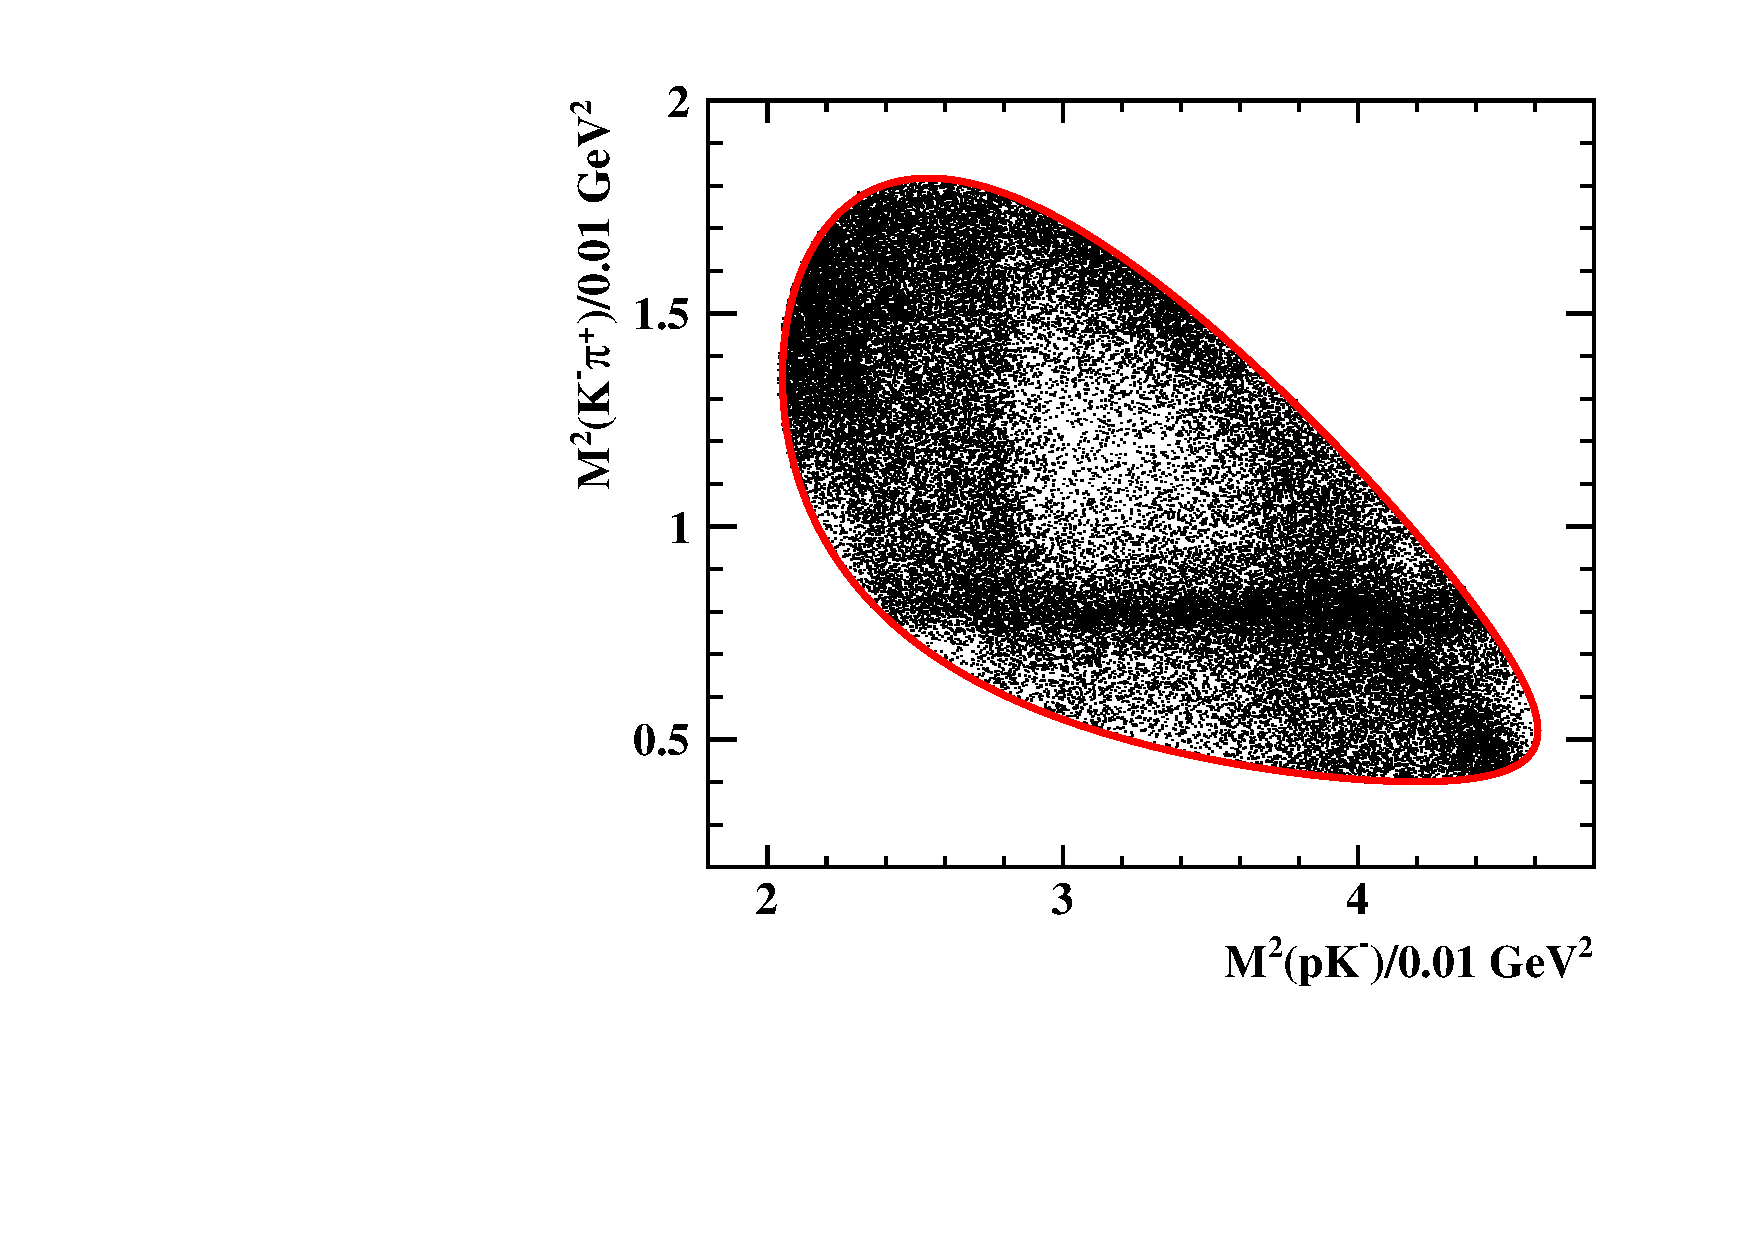
\includegraphics[width=0.48\textwidth]{figure/dalitz/dalitz_Signal_total.pdf}
    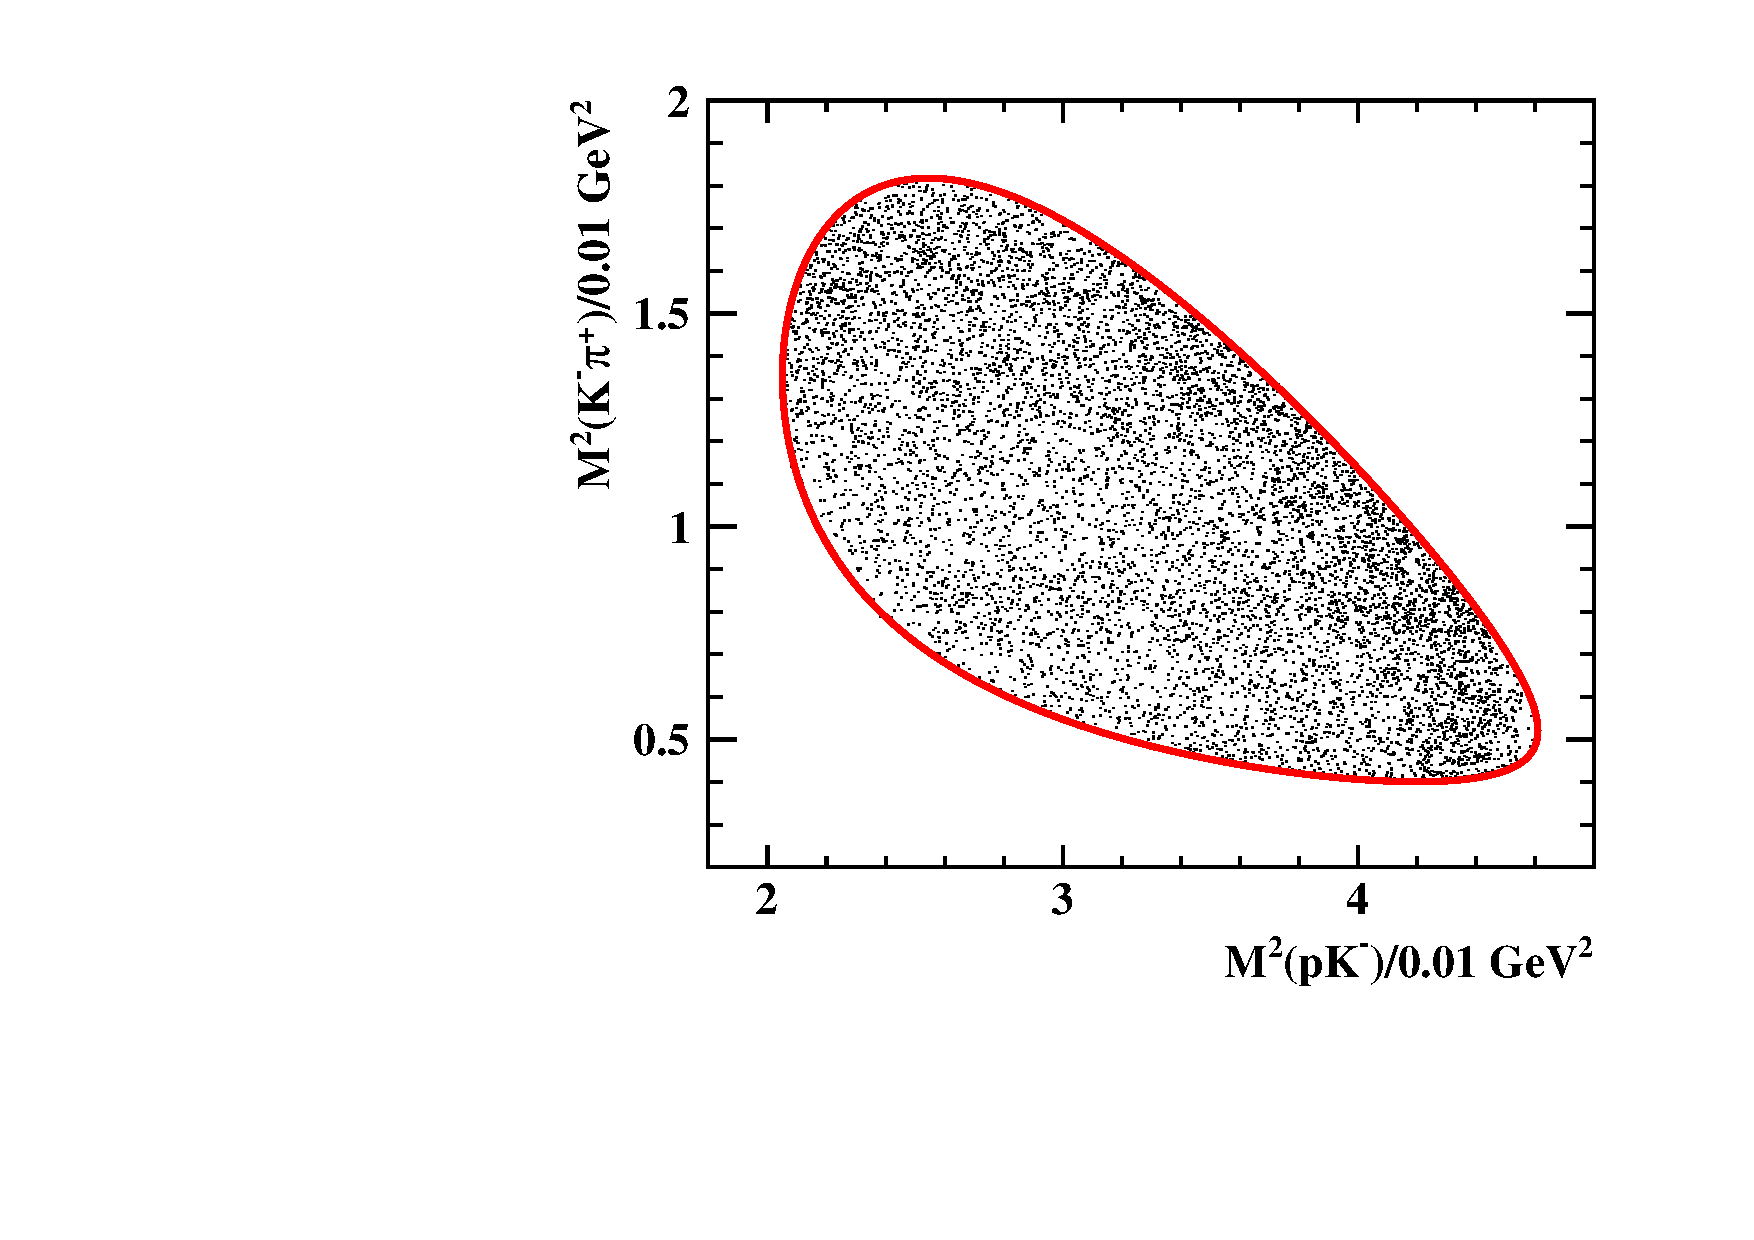
\includegraphics[width=0.48\textwidth]{figure/dalitz/dalitz_Sideband_total.pdf}
    \caption{Dalitz plots for for $M^2(pK^-)$ and $M^2(K^-\pi^+)$ combining all 13 energy points in the $\mbc$ signal region (left) and sideband region (right).}
\label{fig:daltiz_plots}
\end{figure}

\begin{figure}[H]\centering
    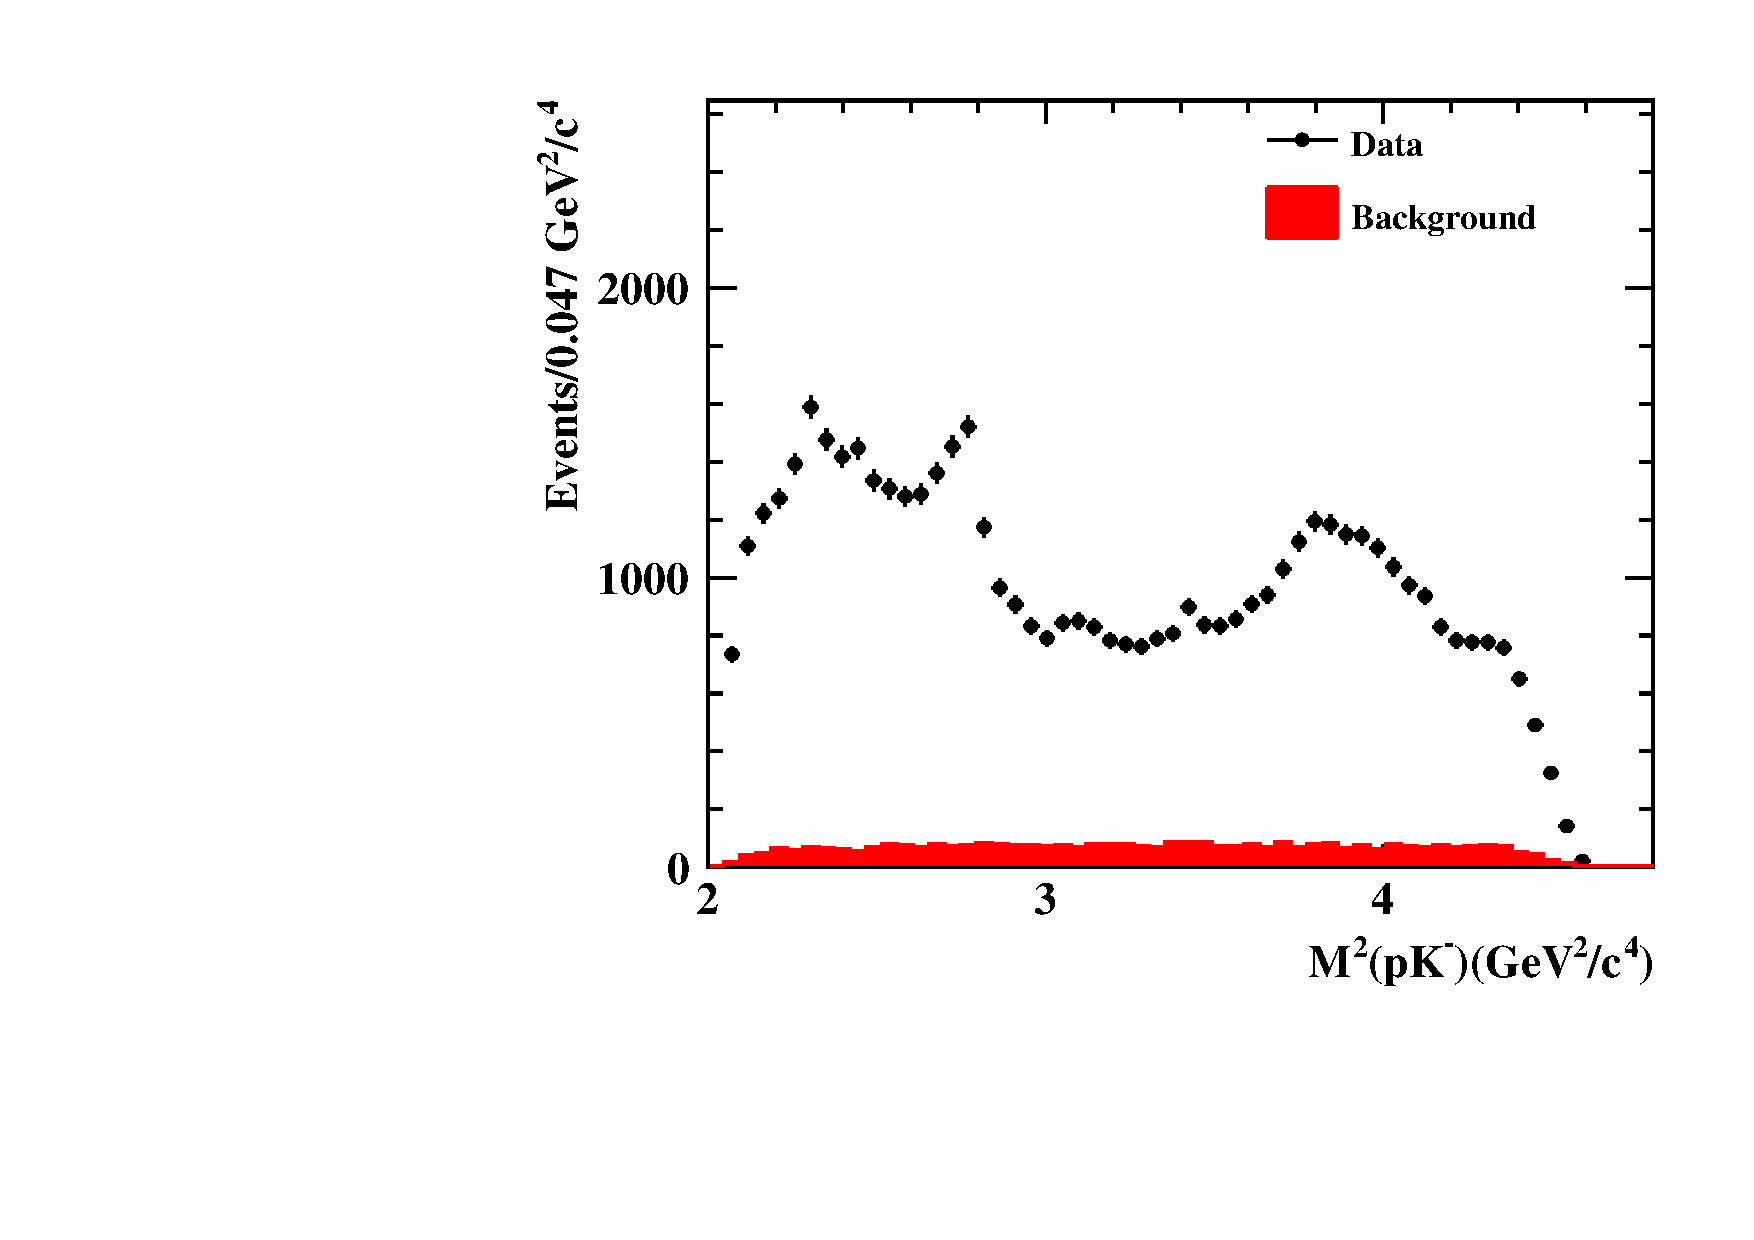
\includegraphics[width=0.32\textwidth]{figure/dalitz/output_data_mc_0_sideband_m2_12_2c_1.pdf}
    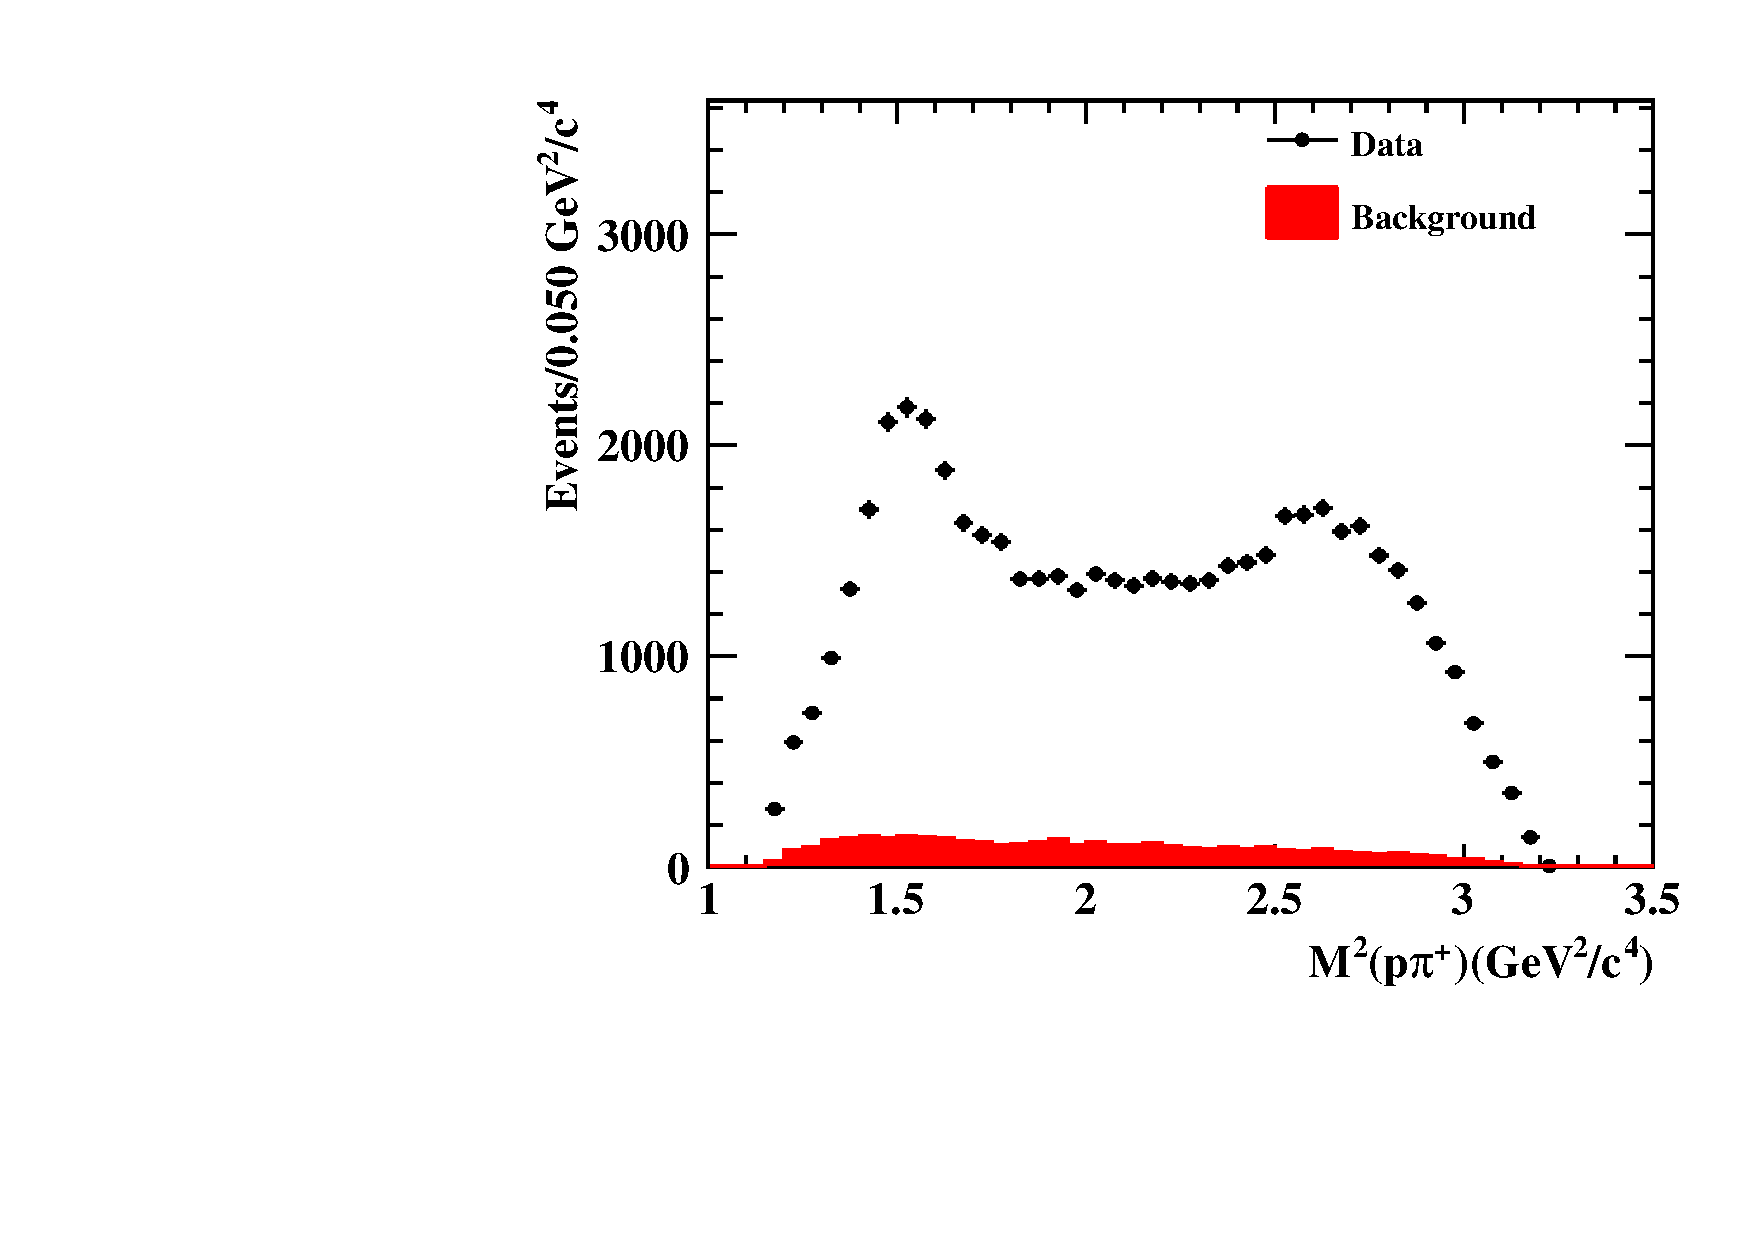
\includegraphics[width=0.32\textwidth]{figure/dalitz/output_data_mc_0_sideband_m2_13_2c_1.pdf}
    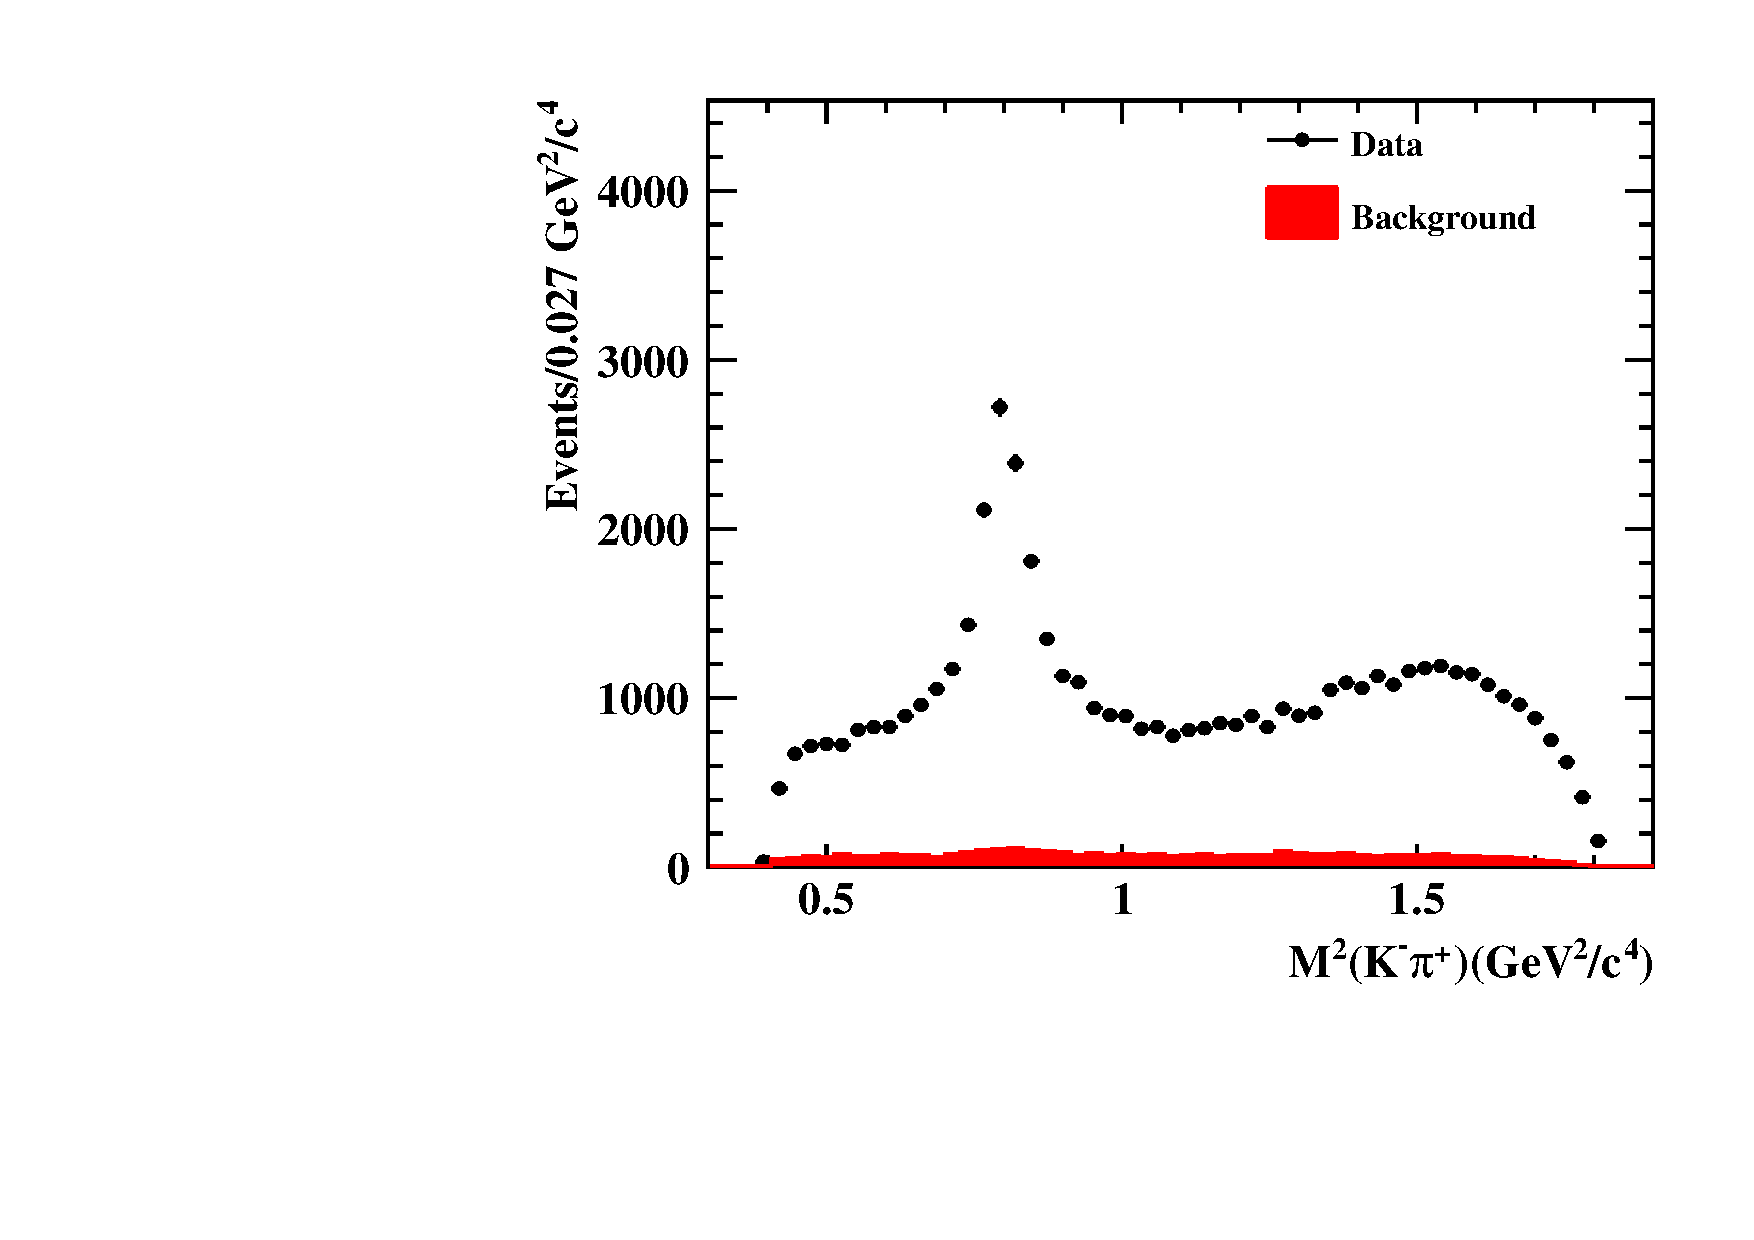
\includegraphics[width=0.32\textwidth]{figure/dalitz/output_data_mc_0_sideband_m2_23_2c_1.pdf}
    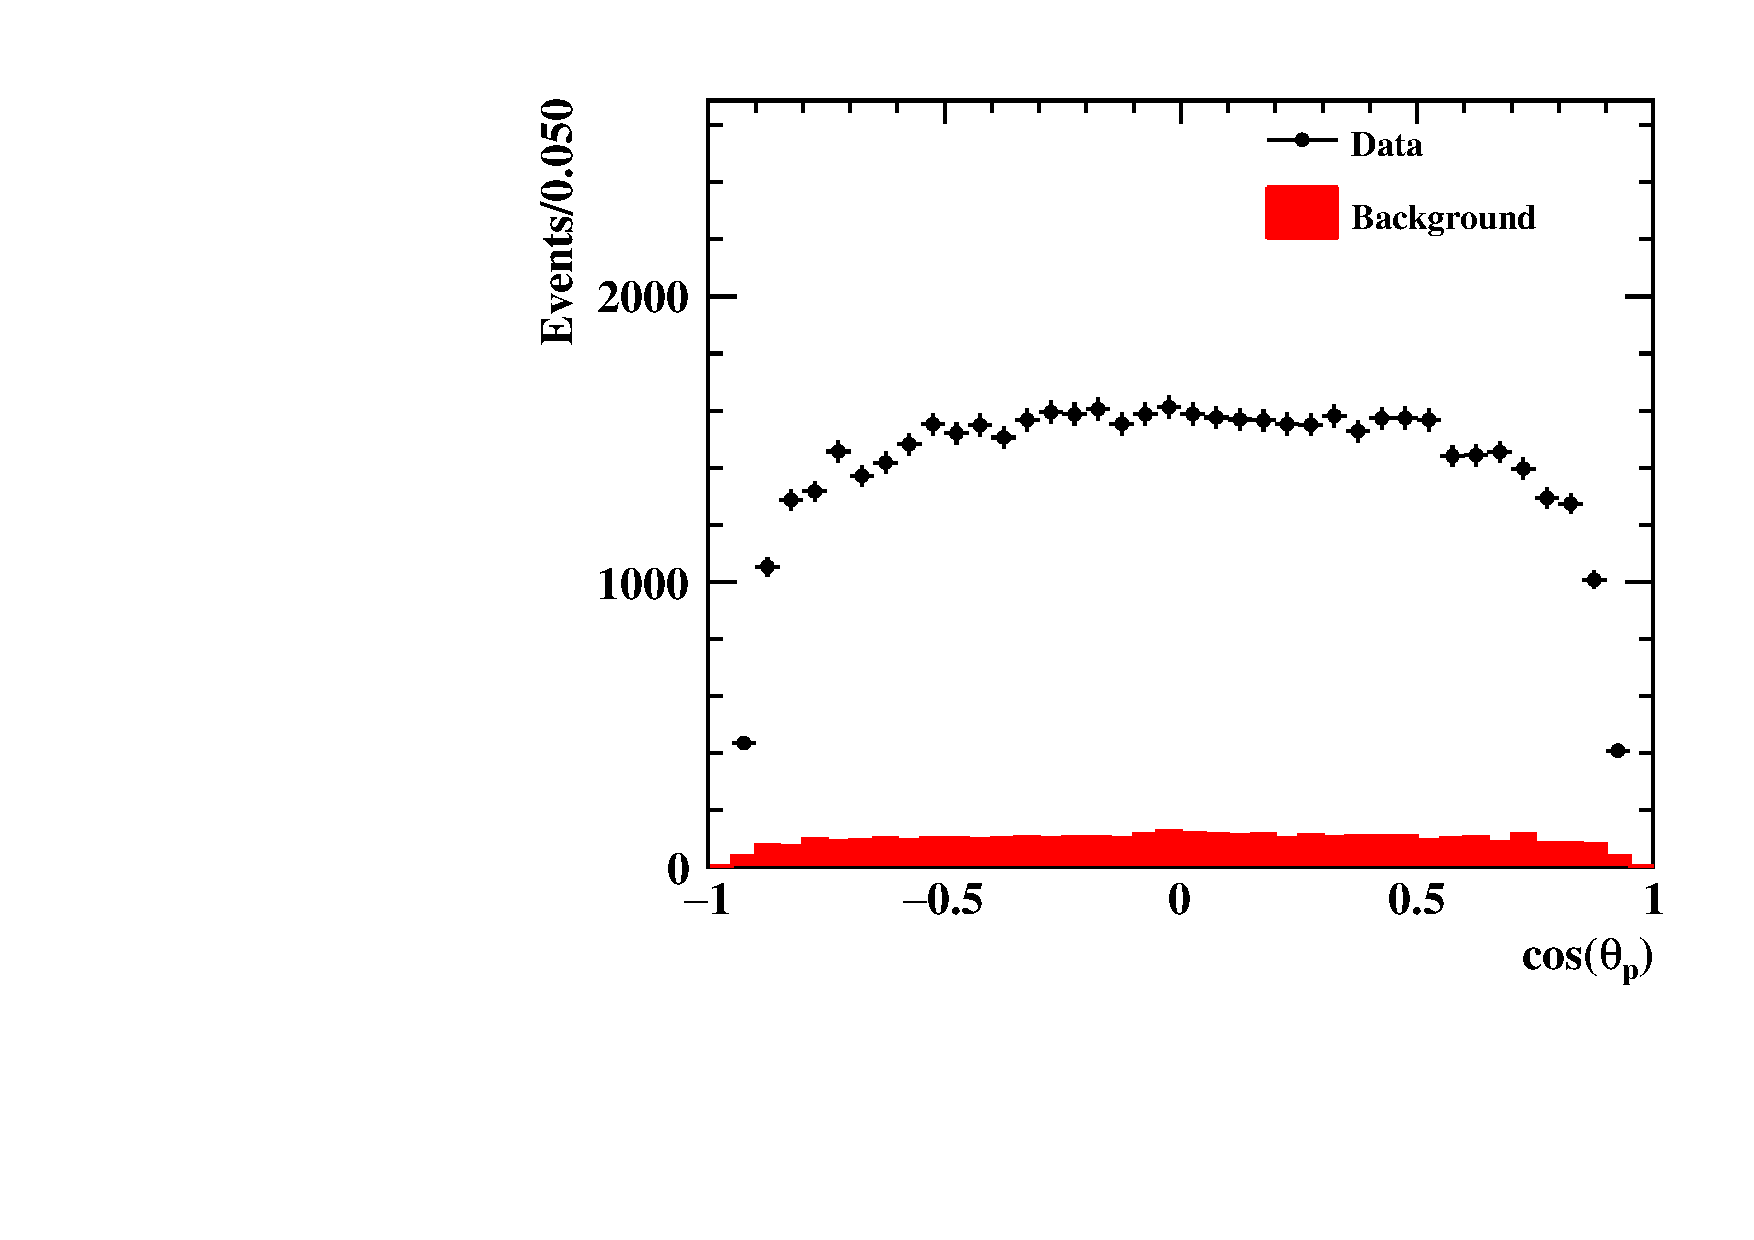
\includegraphics[width=0.32\textwidth]{figure/dalitz/output_data_mc_0_sideband_costheta1_1.pdf}
    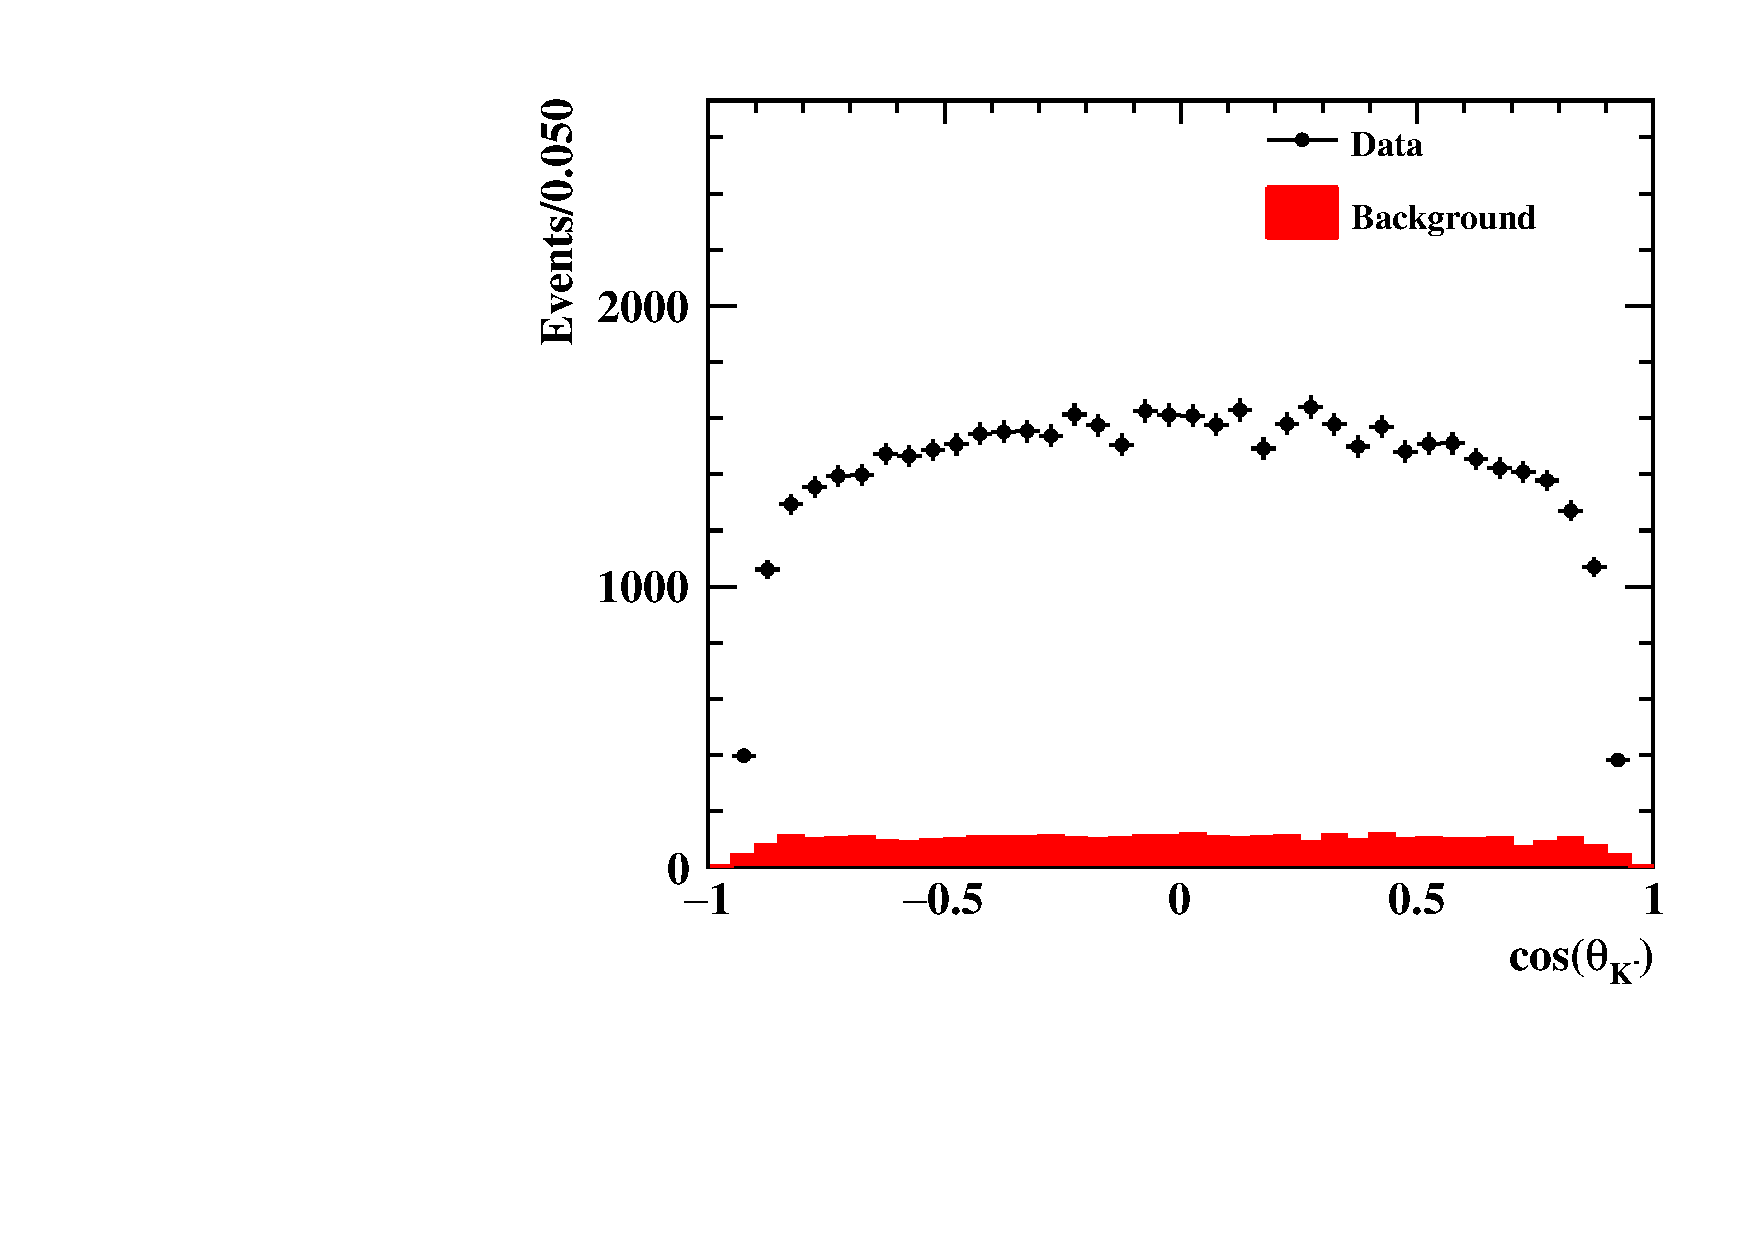
\includegraphics[width=0.32\textwidth]{figure/dalitz/output_data_mc_0_sideband_costheta2_1.pdf}
    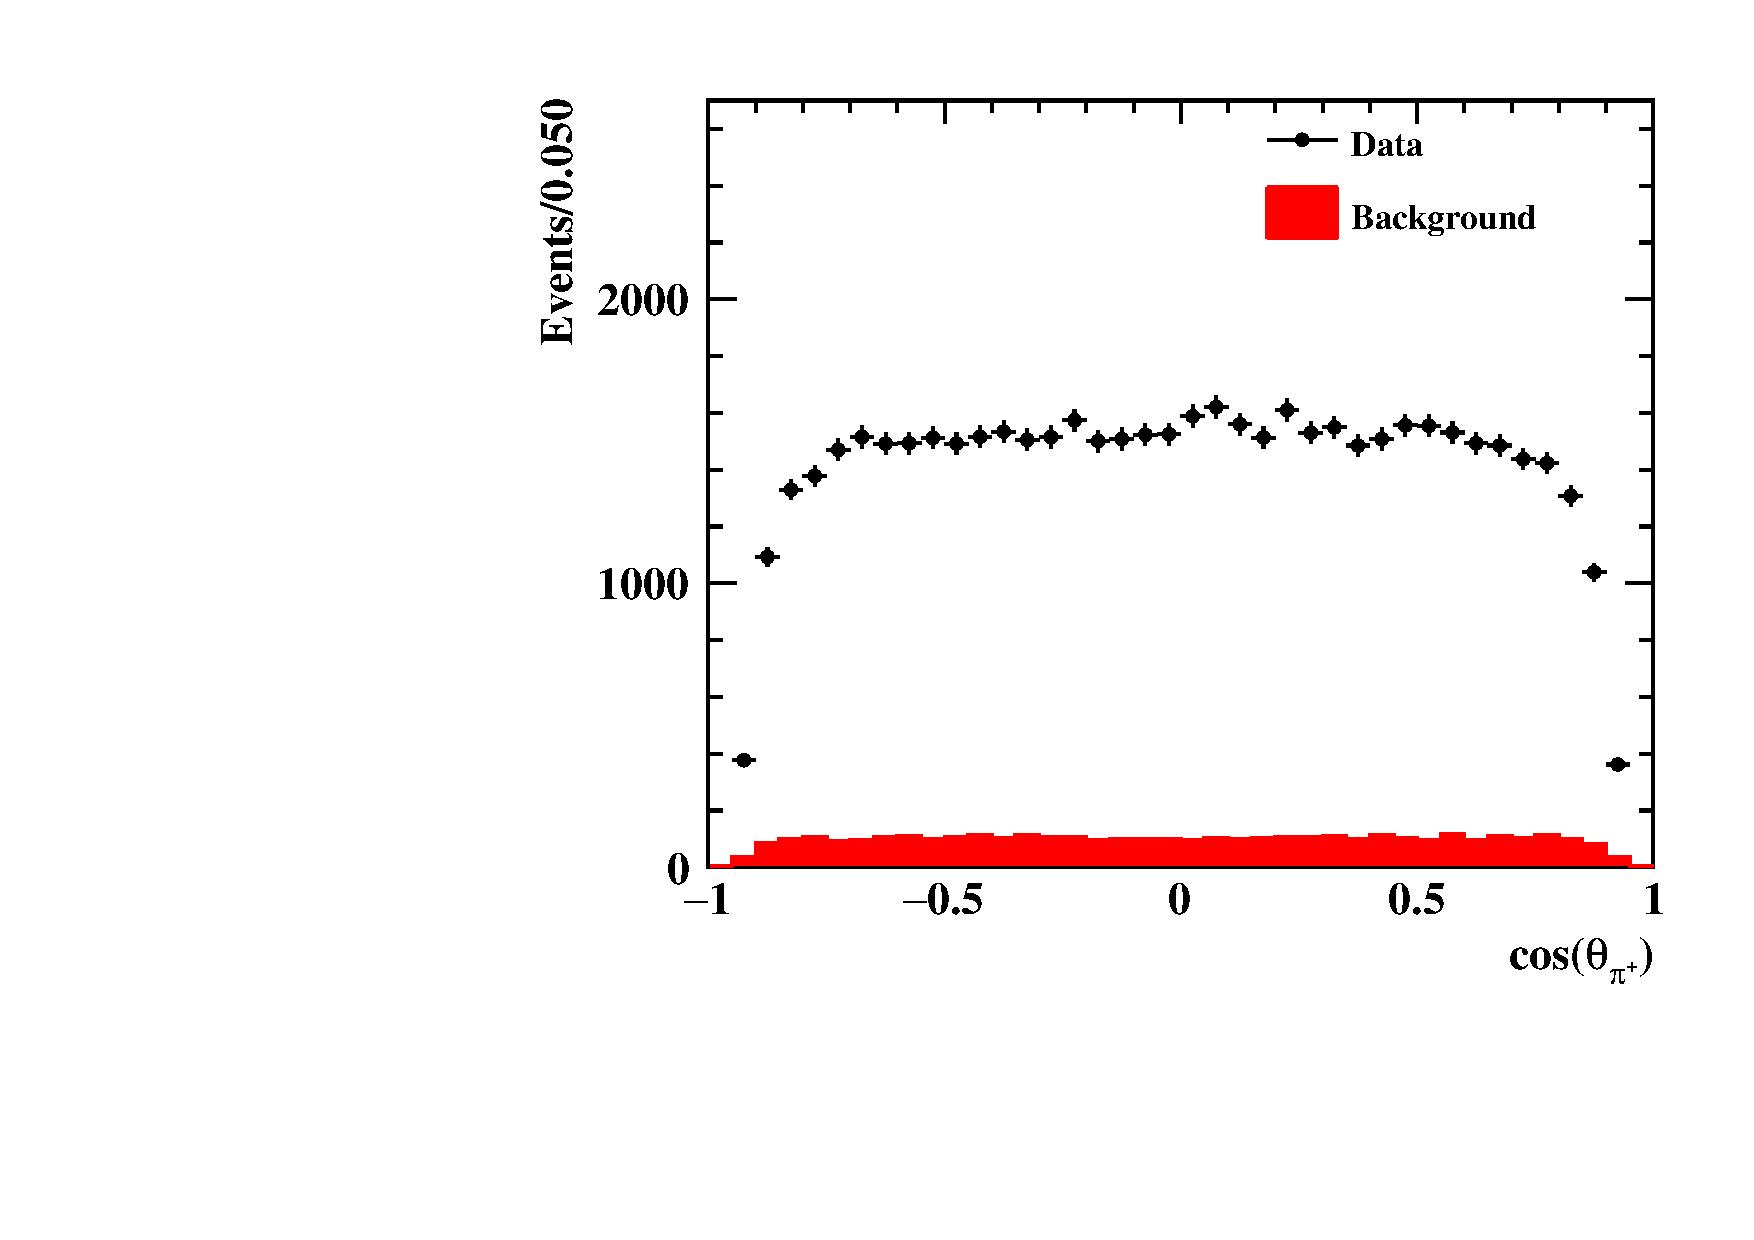
\includegraphics[width=0.32\textwidth]{figure/dalitz/output_data_mc_0_sideband_costheta3_1.pdf}
    \caption{Distributions of the squared two-body invariant mass and polar angles for the selected charged tracks.}
\label{fig:projected_plots}
\end{figure}

\subsection{Helicity amplitude}
\label{sec:helicity_amplitude}
In this analysis, the decay amplitude is constructed using the helicity amplitude formalism~\cite{Chung:186421,Richman:153636} and implemented based on the TF-PWA\footnote[1]{Source codes are available in \hyperlink{github}{https://github.com/jiangyi15/tf-pwa}} package. All final state particles are boosted to the c.m. frame of $e^+e^-$. Under the assumption of CP conservation, the parameters of $\lcm$ amplitudes are related to those of $\lcp$ by performing a parity transformation, where the momenta of $\lcm$ are reversed. 
%Given the assumption of CP conservation, the amplitude of $\lcm$ is the same as the one of $\lcp$ with corresponding parameters performed by the parity transformation.
For process of $e^+e^- \to \gamma^* \to \lcp\lcm$ with $\lcp \to pK^-\pi^+$, its full decay amplitude is formed by the following three decay chains:
\begin{itemize}
    \item $e^+e^- \to \gamma^* \to \lcp\lcm$, $\lcp \to \Lambda^*\pi^+$, $\Lambda^* \to pK^-$, 
    \item $e^+e^- \to \gamma^* \to \lcp\lcm$, $\lcp \to \Delta^{++}K^-$, $\Delta^{++} \to p\pi^+$,
    \item $e^+e^- \to \gamma^* \to \lcp\lcm$, $\lcp \to p\overline{K}^*$, $\overline{K}^* \to K^-\pi^+$.
\end{itemize}
We consider the contributions from $\Lambda^*$, $\Delta^{++}$ and $\overline{K}^*$ resonances according to the PDG~\cite{Workman:2022ynf}. The contribution from $\Sigma^*\to pK^-$ is possible but expected to be suppressed due to the isospin difference of $\Delta I = 1$. It is also hard to separate the contributions between $\Lambda*$ and $\Sigma^*$. In Ref~\cite{LHCb:2022ouv}, the nominal results of amplitude analysis of $\lcp \to p K^-\pi^+$ showed that the dominant contributions were from the $\Lambda^*$ resonances. The $\Sigma^*$ ones were neglected and considered as part of systematic uncertainties. We follow the same strategy and the largest significant $\Sigma^*$ resonances are test and shown in Section~\ref{sec:syst_component}.
%We decide to neglect $\Sigma^*$, which was also done in Ref.~\cite{LHCb:2022ouv}.

The helicity formalism is constructed based on the Isobar model~\cite{Walker:1968xu}, which describes the three-body decay as sequential quasi-two-body decay. For each two body decay $0 \to 1 + 2$, the helicity amplitude can be written as
\begin{equation}\label{eq:2_body_helicity}
    A^{0 \rightarrow 1+2}_{\lambda_{0},\lambda_{1},\lambda_{2}} = H_{\lambda_{1},\lambda_{2}}^{0 \rightarrow 1+2} D^{J_{0}\ast}_{\lambda_{0},\lambda_{1}-\lambda_{2}}(\phi,\theta,0),
\end{equation}
where $H_{\lambda_{1},\lambda_{2}}^{0 \rightarrow 1+2}$ is the helicity coupling and can be expanded using LS coupling formula~\cite{PhysRevD.56.4419,PhysRevD.57.431} to
\begin{equation}
    H_{\lambda_{1},\lambda_{2}}^{0 \rightarrow 1+2} =
\sum_{ls} g_{ls} \sqrt{\frac{2l+1}{2 J_{0}+1}} \langle l0, s\delta|J_{0},\delta\rangle \langle J_{1} J_{2}, \lambda_{1} -\lambda_{2} | s, \delta \rangle \left(\frac{q}{q_0}\right)^l B_{l}'(q, q_0, d), 
\end{equation}
where $g_{ls}$ is the partial wave amplitude, $J_{0,1,2}$ are the spins for particle 0, 1 and 2, $\lambda_{1,2}$ are the helicity for particle 1 and 2, and the $\delta = \lambda_1 - \lambda_2$ is the difference of helicity. $q$ is the momentum of particle 1 in the rest frame of particle 0, which can be written as
\begin{equation}
    q = \frac{\sqrt{[m^2 - (m_1+m_2)^2][m^2 - (m_1 - m_2)^2]}}{2m},
\end{equation}
where $m$, $m_1$ and $m_2$ are the invariant mass of two-body system of particle 1 and 2, the nominal mass values of particle 1 and 2, respectively. $q_0$ is the normalization factor calculated from $q$ with $m$ at resonance nominal mass value. $B_{l}'(q, q_0, d)$ is the reduced Baltt-Weisskopf barrier factor~\cite{Blatt:1952ije}, which is explicitly expressed as
\begin{equation}\label{eq:barrier_factor}
    \begin{split}
    B_{0}'(q, q_0, d) &= 1, \\
    B_{1}'(q, q_0, d) &= \sqrt{\frac{1+(q_0d)^2}{1+(qd)^2}}, \\
    B_{2}'(q, q_0, d) &= \sqrt{\frac{9+3(q_0d)^2+(q_0d)^4}{9+3(qd)^2+(qd)^4}}, \\
    B_{3}'(q, q_0, d) &= \sqrt{\frac{225+45(q_0d)^2+6(q_0d)^4+(q_0d)^6}{225+45(qd)^2+6(qd)^4+(qd)^6}}, \\
    B_{4}'(q, q_0, d) &= \sqrt{\frac{11025+1575(q_0d)^2+135(q_0d)^4+10(q_0d)^6+(q_0d)^8}{11025+1575(qd)^2+135(qd)^4+10(qd)^6+(qd)^8}}
    \end{split}
\end{equation}
$D^{J_{0}\ast}_{\lambda_{0},\lambda_{1}-\lambda_{2}}(\phi,\theta,0)$ is Wigner D-function, where $\theta$ indicates the helicity angle of the decay of resonance and $\phi$ is defined as helicity angle between the decay plane of daughter particle and the one of its mother particle. More details about the definitions of helicity angles can be found in Ref~\cite{Wang:2020giv}. In Eq.~(\ref{eq:barrier_factor}), the radius of centrifugal barrier $d$ is chosen as $d=1/q_r=3.69(\rm{GeV}/c)^{-1}$, which is the same as in Ref.~\cite{BESIII:2019dme}.

The full amplitude of each component is the production of every two-body decay amplitudes and the dynamical part. For the $\Lambda^*(pK^-)$ resonances:   
\begin{equation}
    A_{\lambda_{\gamma^*},\lambda_{\bar{\Lambda}_c^{-}},\lambda_p}^{\Lambda^*} = \sum_{\lambda_{\Lambda_c^+},\lambda_{\Lambda^*}}A_{\lambda_{\gamma^*},\lambda_{\Lambda_c^+},\lambda_{\bar{\Lambda}_c^-}}^{\gamma^* \to \Lambda_c^+\bar{\Lambda}_c^-}A_{\lambda_{\Lambda_c^+},\lambda_{\Lambda^*},0}^{\Lambda_c^+\to\Lambda^*\pi^+}R_{\Lambda^*}(M_{pK^-})A_{\lambda_{\Lambda^*},\lambda_p,0}^{\Lambda^*\to pK^-}.
\end{equation}
For the $\Delta^{++}(p\pi^+)$ resonances: 
\begin{equation}
    A_{\lambda_{\gamma^*},\lambda_{\bar{\Lambda}_c^{-}},\lambda_p}^{\Delta^{++}} = \sum_{\lambda_{\Lambda_c^+},\lambda_{\Delta^{++}}}A_{\lambda_{\gamma^*},\lambda_{\Lambda_c^+},\lambda_{\bar{\Lambda}_c^-}}^{\gamma^* \to \Lambda_c^+\bar{\Lambda}_c^-}A_{\lambda_{\Lambda_c^+},\lambda_{\Delta^{++}},0}^{\Lambda_c^+\to\Delta^{++}K^-}R_{\Delta^{++}}(M_{p\pi^+})A_{\lambda_{\Delta^{++}},\lambda_p,0}^{\Delta^{++}\to p\pi^+}.
\end{equation}
For the $\overline{K}^*(K^-\pi^+)$ resonances:
\begin{equation}
    A_{\lambda_{\gamma^*},\lambda_{\bar{\Lambda}_c^{-}},\lambda_p}^{\overline{K}^{*0}} = \sum_{\lambda_{\Lambda_c^+},\lambda_{\overline{K}^{*0}}}A_{\lambda_{\gamma^*},\lambda_{\Lambda_c^+},\lambda_{\bar{\Lambda}_c^-}}^{\gamma^* \to \Lambda_c^+\bar{\Lambda}_c^-}A_{\lambda_{\Lambda_c^+},\lambda_{\overline{K}^{*0}},\lambda_p}^{\Lambda_c^+\to p \overline{K}^{*0}}R_{\overline{K}^{*0}}(M_{K^-\pi^+})A_{\lambda_{\overline{K}^{*0}},0,0}^{\overline{K}^{*0}\to K^-\pi^+}.
\end{equation}
The dynamic parts, $R_{\Lambda^*}(pK^-)$, $R_{\Delta^{++}}(p\pi^+)$ and $R_{\overline{K}^*}(K^-\pi^+)$, include different models and will be explained in Section~\ref{sec:resonances}.
The total amplitude is represented by summing all possible resonances as:
\begin{equation}\label{eq:total_amplitude}
    \begin{split}
    A_{\lambda_{\gamma^*},\lambda_{\bar{\Lambda}_c^{-}}, \lambda_p} &=  A_{\lambda_{\gamma^*},\lambda_{\bar{\Lambda}_c^{-}},\lambda_p}^{\Lambda^*} \\
    &+ \sum_{\lambda^{\prime}_{\bar{\Lambda}_c^-},\lambda^{\prime}_p}(\sum A_{\lambda_{\gamma^*},\lambda^{\prime}_{\bar{\Lambda}_c^{-}},\lambda^{\prime}_p}^{\Delta^{++}})D_{\lambda^{\prime}_{\bar{\Lambda}_c^-}, \lambda_{\bar{\Lambda}_c^-}}^{1/2}(\alpha_{\bar{\Lambda}_c^-}, \beta_{\bar{\Lambda}_c^-}, \gamma_{\bar{\Lambda}_c^-})D_{\lambda^{\prime}_{p}, \lambda_{p}}^{1/2}(\alpha_{p}, \beta_{p}, \gamma_{p})\\
    &+ \sum_{\lambda^{\prime}_{\bar{\Lambda}_c^-},\lambda^{\prime}_p}(\sum A_{\lambda_{\gamma^*},\lambda^{\prime}_{\bar{\Lambda}_c^{-}},\lambda^{\prime}_p}^{\overline{K}^*})D_{\lambda^{\prime}_{\bar{\Lambda}_c^-}, \lambda_{\bar{\Lambda}_c^-}}^{1/2}(\alpha^{\prime}_{\bar{\Lambda}_c^-}, \beta^{\prime}_{\bar{\Lambda}_c^-}, \gamma^{\prime}_{\bar{\Lambda}_c^-})D_{\lambda^{\prime}_{p}, \lambda_{p}}^{1/2}(\alpha^{\prime}_{p}, \beta^{\prime}_{p}, \gamma^{\prime}_{p}),
    \end{split}
\end{equation}
where the extra D-functions are added to align the final $\bar{\Lambda}_c^-$ and proton final states, correcting the helicities of $\bar{\Lambda}_c^-$ and proton in different chains. In the helicity amplitude Eq.~(\ref{eq:2_body_helicity}), the helicities of particle 1 and particle 2 are defined by the rotation ($\theta$, $\phi$) and boost sequences from initial states to final states. So it is necessary to include the extra D-functions in the sum of the amplitude within the same helicity. More details can be found in Ref.~\cite{BESIII:2022udq}.

\subsection{Resonance components and models}
\label{sec:resonances}
The full amplitude model is built by summing helicity amplitudes of all possible intermediate resonances, as indicated in Eq.~(\ref{eq:total_amplitude}). We consider the contributions from $\Lambda^*$, $\Delta^{++}$ and $\overline{K}^*$ and use the results in Ref.~\cite{LHCb:2022ouv} as starting point. The models and corresponding parameters are summarized in Table~\ref{tab:parameters}. The resolution effects are studied and documented in Appendix~\ref{app:resolution}.

\begin{table}[htbp]
    \centering
    \caption{List of $\Lambda^*$, $\Delta^{++}$ and $\overline{K}^*$ resonances considered in the amplitude model. The model parameters are taken according to the PDG~\cite{Workman:2022ynf} and LHCb's results\cite{LHCb:2022ouv}.}
    \label{tab:parameters}
    \begin{tabular}{ccccc}
        \hline\hline
        Resonance & $J^P$ & Mass (MeV)  & Width (MeV) & Model \\\hline
        $\Lambda(1405)$ & $1/2^-$ & 1405.1 & 50.5  & Flatte \\
        $\Lambda(1520)$ & $3/2^-$ & 1518.5 & 15.2  & Relativistic Breit-Wigner\\
        $\Lambda(1600)$ & $1/2^+$ & 1630   & 250   & Relativistic Breit-Wigner\\
        $\Lambda(1670)$ & $1/2^-$ & 1670   & 30    & Relativistic Breit-Wigner\\
        $\Lambda(1690)$ & $3/2^-$ & 1690   & 70    & Relativistic Breit-Wigner\\
        $\Lambda(2000)$ & $1/2^-$ & 1988   & 179   & Relativistic Breit-Wigner\\\hline
        $\Delta(1232)^{++}$ & $3/2^+$ & 1232 & 117 & Relativistic Breit-Wigner\\
        $\Delta(1600)^{++}$ & $3/2^+$ & 1640 & 300 & Relativistic Breit-Wigner\\
        $\Delta(1620)^{++}$ & $1/2^-$ & 1610 & 130 & Relativistic Breit-Wigner\\ 
        $\Delta(1700)^{++}$ & $3/2^-$ & 1690 & 380 & Relativistic Breit-Wigner\\\hline 
        $\overline{K}^*_0(700)$  & $0^+$ & 824 & 478 & Bugg\\
        $\overline{K}^*(892)$    & $1^-$ & 895.5 & 47.3 & Relativistic Breit-Wigner\\
        $\overline{K}^*_0(1430)$ & $0^+$ & 1375  & 190  & Bugg\\ 
        \hline\hline
    \end{tabular}
\end{table}

By default the resonances are parameterized by relativistic Briet-Wigner formula:
\begin{equation}
    R(m) = \frac{1}{m_0^2 - m^2 - im_0\Gamma(m)},
\end{equation} 
where the mass dependent width is
\begin{equation}
    \label{eq:bw_width}
    \Gamma(m) = \Gamma_0\left(\frac{q}{q_0}\right)^{2l+1}\frac{m_0}{m}B_l^{\prime 2}(q,q_0,d).
\end{equation}

The spin-zero $\overline{K}^*$ resonances, $\overline{K}^*(700)$ and $\overline{K}^*(1430)$, are described by a parameterization presented in Ref.~\cite{Bugg:2005xx}, which is also called Bugg lineshape. It consists of a Briet-Wigner lineshape, where the mass dependent width is replaced by
\begin{equation}
    \Gamma(m) = \frac{m^2-s_A}{m_0^2 - s_A}\Gamma_0e^{-\gamma m^2},
\end{equation}
which features a singularity (Adler zero) at $s_A = m_K^2 - 0.5m_\pi^2$ and exponential form factor on the $K\pi$ width driven by the parameter $\gamma$. The $\gamma$ parameters are fixed at 0.94 GeV$^{-2}$ and 0.02 GeV$^{-2}$ for $\overline{K}^*(700)$ and $\overline{K}^*(1430)$ respectively, according to Ref.~\cite{LHCb:2022ouv}. Comparing to the original parameterization in Ref.~\cite{Bugg:2005xx}, the additional overall exponential form factor and the opening of $K\eta$, $K\eta^\prime$ decay channels are neglect in the fit.

The $\Lambda(1405)$ resonance has the pole mass below the $pK^-$ threshold, which is parameterized by a Flatt\'e lineshape~\cite{Flatte:1976xu}. This lineshape describe the opening of the $pK$ decay channel in addition to the $\Sigma\pi$ decay. It consists of a Breit-Wigner lineshape with total width being the sum of the widths associated to the two decay channels,
\begin{equation}
    \Gamma(m) = \Gamma_{pK}(m) + \Gamma_{\Sigma\pi}(m),
\end{equation}
where $\Gamma_{pK}(m)$ and $\Gamma_{\Sigma\pi}(m)$ are calculated by Eq.~(\ref{eq:bw_width}) with $q_0$ derived from the decay of $\Sigma\pi$. $\Gamma_0$ is fixed at the total width of $\Lambda(1405)$ resonance in both term in the fit.
%The detailed formula can be written as:
%\begin{equation}
%    R(m) = \frac{1}{m^2 - m_0^2 - i(g_1\rho_{K\pi}(m) + g_2\rho_{\Sigma\pi})}, 
%\end{equation}
%where $g_1$ and $g_2$ are the coupling constant of $\Lambda(1405)$ to $pK$ and $\Sigma\pi$ channels, $\rho_{pK}$ and $\rho_{\Sigma\pi}$ are the available phase space for the the channels with $\rho = q/m$. 
%Comparing to the relativistic Breit-Wigner lineshape, the total width of $\Lambda(1405)$ is the sum of the widths of the two decay channels,
%\begin{equation}
%    \Gamma(m) = \Gamma_{pK}(m) + \Gamma_{\Sigma\pi}(m).
%\end{equation}
 

\subsection{Likelihood function and construction}
\label{sec:likelihood}
Using the total amplitude in Eq.~(\ref{eq:total_amplitude}), the probability distribution is defined as
\begin{equation}
    P(p_j) = \frac{\varepsilon(p_j)|A(p_j)|^2R_4(p_j)}{\int\varepsilon(p_j)|A(p_j)|^2R_4(p_j)\mathrm{d}p_j}, \,\,|A|^2 = \sum_{\lambda_{\gamma^*},\lambda_{\bar{\Lambda}_c^-}, \lambda_p}|A_{\lambda_{\gamma^*},\lambda_{\bar{\Lambda}_c^-},\lambda_p}|^2,
\end{equation}
where $\varepsilon(p_j)$ is the detection efficiency as a function of four momentum ($p_j$) of final particles. The integration part in the denominator is calculated by the sum of the phase space MC mentioned in Section~\ref{sec:sample} 
\begin{equation}\label{eq:mc_integration}
    \int\varepsilon(p_j)|A(p_j)|^2R_4(p_j)\mathrm{d}p_j \varpropto \frac{1}{N_\mathrm{PHSP}}\sum_{i \in \mathrm{{PHSP}}} |A(x_i)|^2.
\end{equation}
The negative log likelihood (NLL) is formed using the background subtraction method:
\begin{equation}\label{eq:nll}
    -\ln L = -\alpha\left[\sum_{i\in\mathrm{data}}\ln P(x_i) - w^\prime_\mathrm{bkg}\sum_{j\in sideband} \ln P(x_j)\right],
\end{equation}
where the background extrapolation factor $w^{\prime}_\mathrm{bkg} = w_\mathrm{bkg} \cdot N_\mathrm{data}/N_\mathrm{sideband}$ and $w_\mathrm{bkg}$ is the background fraction within $\mbc$ signal reigon obtained from the fit on $\mbc$. The normalization factor $\alpha$~\cite{Langenbruch_2022} is defined as 
%The normalization factor~\cite{Langenbruch_2022} used to correct errors is expressed as
\begin{equation}
    \alpha = \frac{N_\mathrm{data} - N_\mathrm{sideband}w^{\prime}_\mathrm{bkg}}{N_\mathrm{data} + N_\mathrm{sideband}w^{\prime 2}_\mathrm{bkg}}.
\end{equation}
It is used to include the effect of weights in the determination of uncertainties. Without considering it, uncertainties calculation will be underestimated.
The NLLs are created for each energy points with shared parameters arising from the decays of $\lcp$ and resonance states and separated partial wave amplitudes $g_{ls}$ in the process of $e^+e^-\to\gamma^*\to \lcp\lcm$. The joint NLL is obtained by summing all NLLs from each energy points. 

After minimizing the joint NLL, the parameters error matrix is calculated by the inverse hessian matrix:
\begin{equation}\label{eq:ff}
    V_{ij}^{-1} = - \frac{\partial^2 \ln L}{\partial \theta_i \partial \theta_j},
\end{equation}
where $\theta_i$ is the $i$-th floated parameters in the likelihood formula. This is the standard form of the error matrix in the maximum likelihood fit.

The fit fraction (FF) of each resonance state is calculated using
\begin{equation} \label{eq:ff2}
    \mathrm{FF}_{i} = \frac{\int |A_i|^2\mathrm{d}\Phi}{\int |\sum_k A_k|^2\mathrm{d}\Phi} \varpropto \frac{\sum_{j\in\mathrm{PHSP}}|A_i(x_j)|^2}{\sum_{j\in\mathrm{PHSP}}|\sum_k A_k(x_j)|^2},
\end{equation}
where $A_i$ is the amplitude of $i$-th component and the integration is calculated by summing the truth level PHSP MC samples without considering the detector response. The interference part between $i$-th and $j$-th components is derived by
\begin{equation}\label{eq:ff3}
    \mathrm{FF}_{i,j} = \frac{\int |A_i + A_j|^2\mathrm{d}\Phi}{\int |\sum_k A_k|^2\mathrm{d}\Phi} - \mathrm{FF}_i - \mathrm{FF}_j.
\end{equation}
The statistical uncertainties for FF are obtained with the standard form of error propagation. Let \textbf{\emph{Y}} be the variable whose error needs to be calculated, \textbf{\emph{X}} be the variables with a corresponding error matrix $V_{ij}$ in Eq.~(\ref{eq:ff}) and $\boldsymbol{\mu}$ be the nominal results of the floating variables \textbf{\emph{X}}, the variance of \textbf{\emph{Y}} is estimated as
\begin{equation}
    \sigma_Y^2 = \sum_{ij}\left(\frac{\partial Y}{\partial X_i}\right)_{\boldsymbol{X} = \boldsymbol{\mu}} V_{ij}\left(\frac{\partial Y}{\partial X_j}\right)_{\boldsymbol{X}=\boldsymbol{\mu}}.
\end{equation}
A validation test is performed using high-dimensional sampling considering the error matrix and details are documented in Appendix~\ref{app:ff_error}.

\subsection{Nominal fit results}
\label{sec:nominal_fit}
As a starting point, we use the nominal choice of resonances and fix their parameters as benchmark model based on Ref.~\cite{LHCb:2022ouv}. The statistical significance test is performed for additional $\Lambda^*$, $\Sigma^*$ and $\Delta^{++}$ resonance states, including $\Lambda(1800)$, $\Lambda(1810)$, $\Lambda(1820)$, $\Lambda(1830)$, $\Lambda(1890)$, $\Sigma(1670)$, $\Sigma(1750)$, $\Sigma(1775)$, $\Sigma(1915)$ and $\Delta(1620)^{++}$ with certain experimental evidence for resonance existence in the PDG~\cite{Workman:2022ynf}.
%with a score of at least three stars in PDG~\cite{Workman:2022ynf}. 
The statistical significance is calculated using the change of the NLL values with and without each additional resonance, by taking into account the change of the number of degree of freedom (NDF). The results show that $\Delta(1620)^{++}$ has a large significance with 5.7$\sigma$, while all the other components have significance values below 5$\sigma$. The additional resonances will be considered in the systematic uncertainties of model components in Section~\ref{sec:syst_component}. 
The final components of the nominal model and corresponding parameters are shown in Table~\ref{tab:parameters}. The statistical significance values are listed in Table~\ref{tab:nom_significance} for each component in the nominal model. The constructed joint NLL includes 80 floated parameters, including (54) shared amplitudes and (26) separated partial wave amplitude $g_{ls}^{\gamma^*}$. The shared parameters are $g_{ls}$ of the decay of $\lcp \to Rh$ and $R$, where $R$ is the intermediate resonance and $h$ is the remaining final particle. They are expected to be identical in all 13 energy points. The fit quality is measured by a $\chi^2$ test performed over a 5-dimensional binning of phase space, which describe the amplitude of $\lcp\to p K^-\pi^+$. The selected variables are two Dalitz variables ($M^2(pK^-)$, $M^2(K^-\pi^+)$) and three helicity angles ($\phi_{p}^{\lcp}$, $\cos(\theta_{p})$ and $\phi_{K^{-}}^{\bar{K^{*}}}$), where $\phi_{p}^{\lcp}$ is the angle between the plane made by $p$ and $\bar{K}^*$ and $\lcp$ production plane, $\cos(\theta_{p})$ is the angle between the momenta of $p$ and $\lcp$ in the $\lcp$ rest frame, $\phi_{K^{-}}^{\bar{K^{*}}}$ is the angle between the planes made by $K^-\pi^+$ and $p \bar{K}^*$. An adaptive binning technique is employed to guarantee similar number of data events in each bin. The projected invariant mass distributions and helicity angles are shown in Figure~\ref{fig:pwa_nominal_comb} combining all 13 energy points.

\begin{figure}[htbp]\centering
    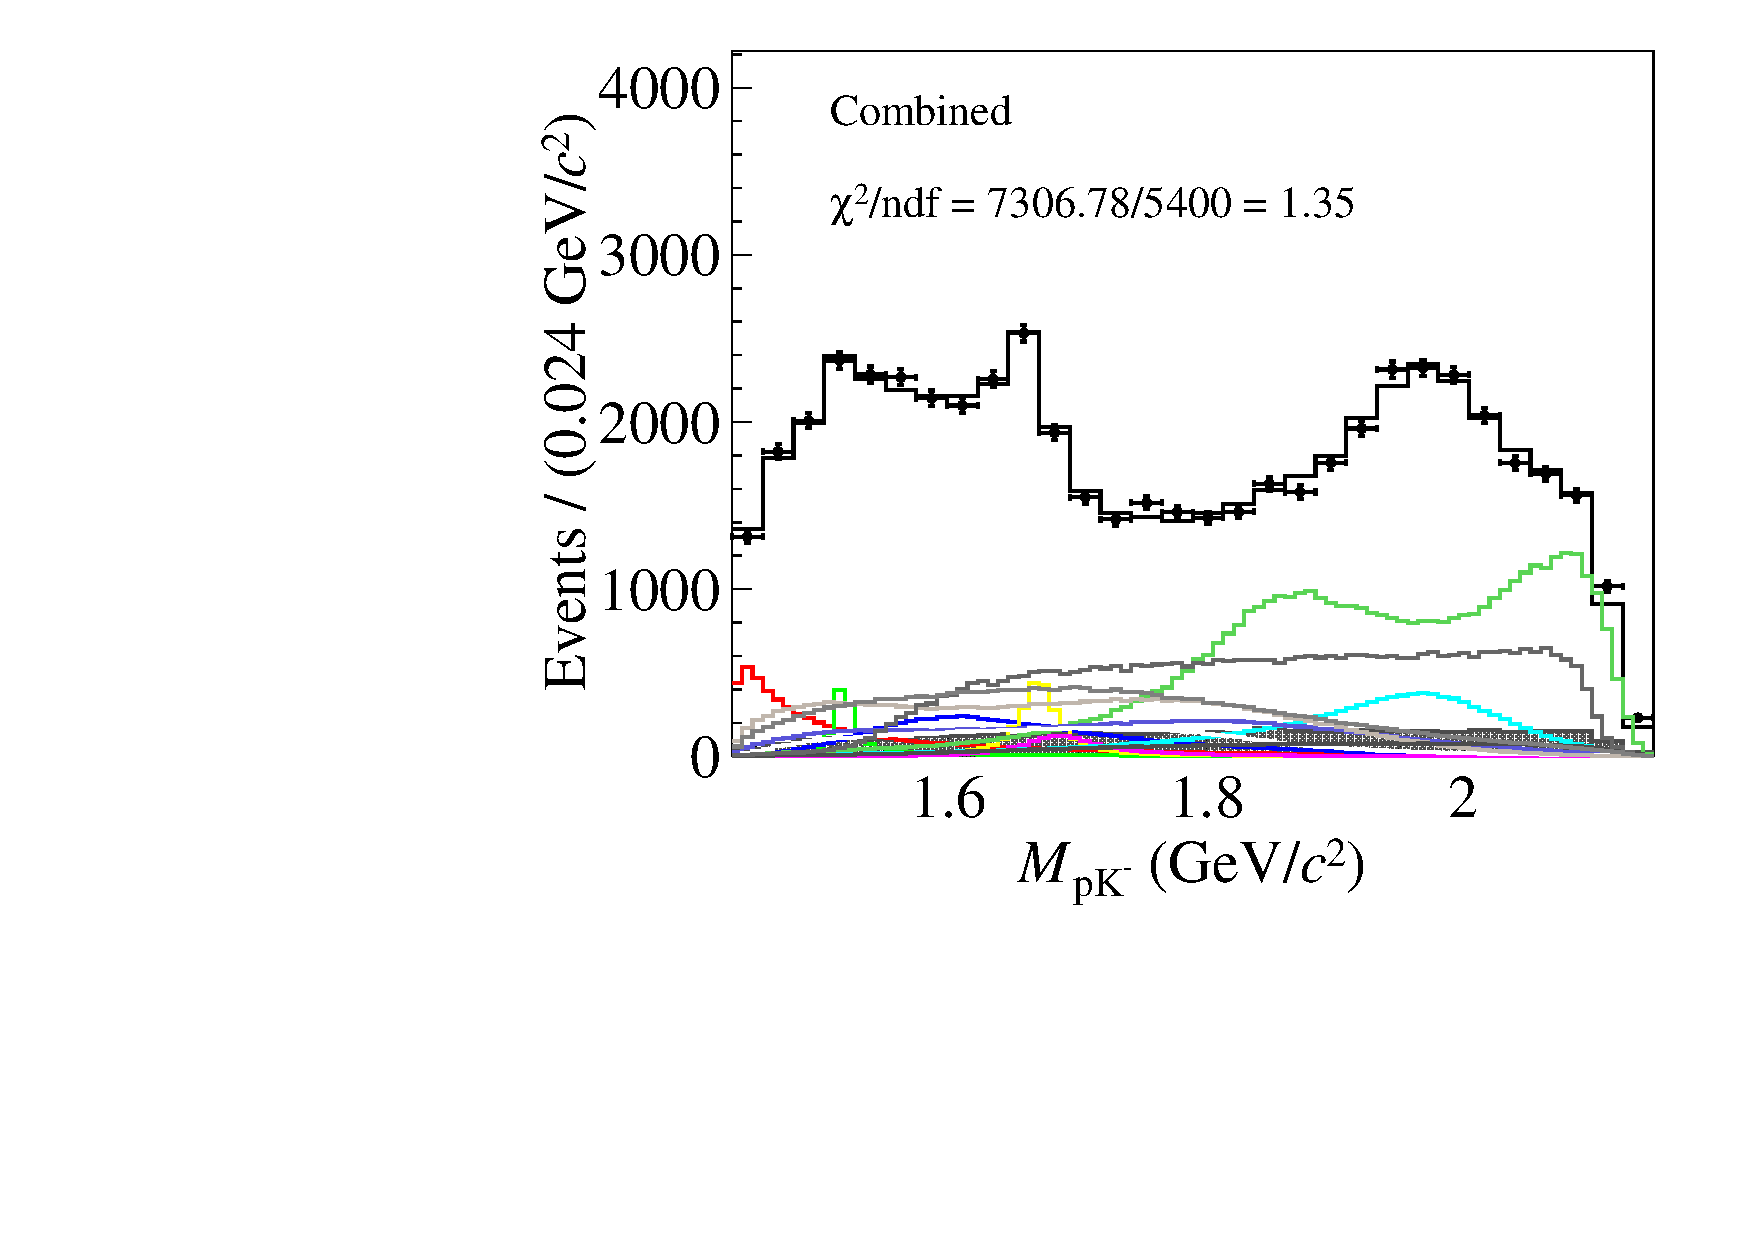
\includegraphics[width=0.32\textwidth]{figure/pwa_nominal/data_all_m_R_BC.pdf}
    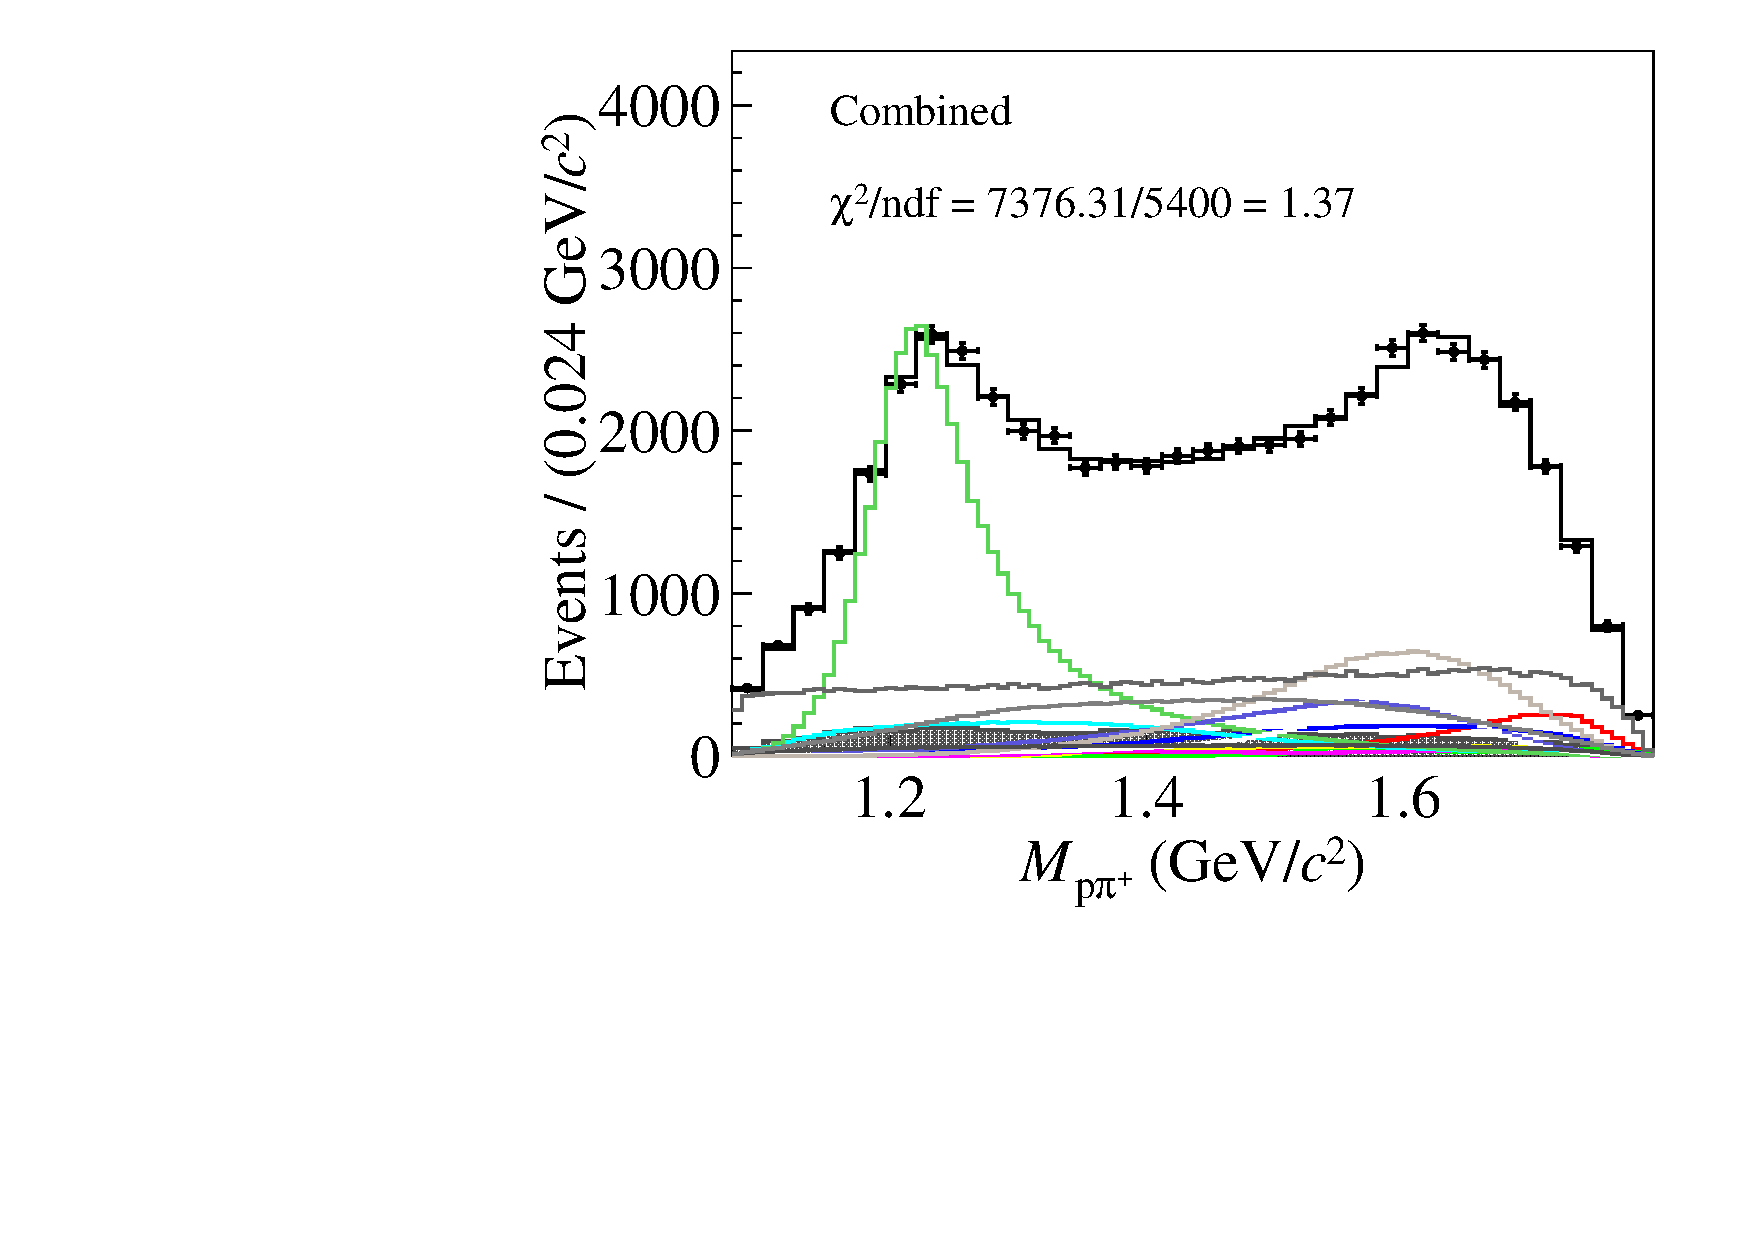
\includegraphics[width=0.32\textwidth]{figure/pwa_nominal/data_all_m_R_BD.pdf}
    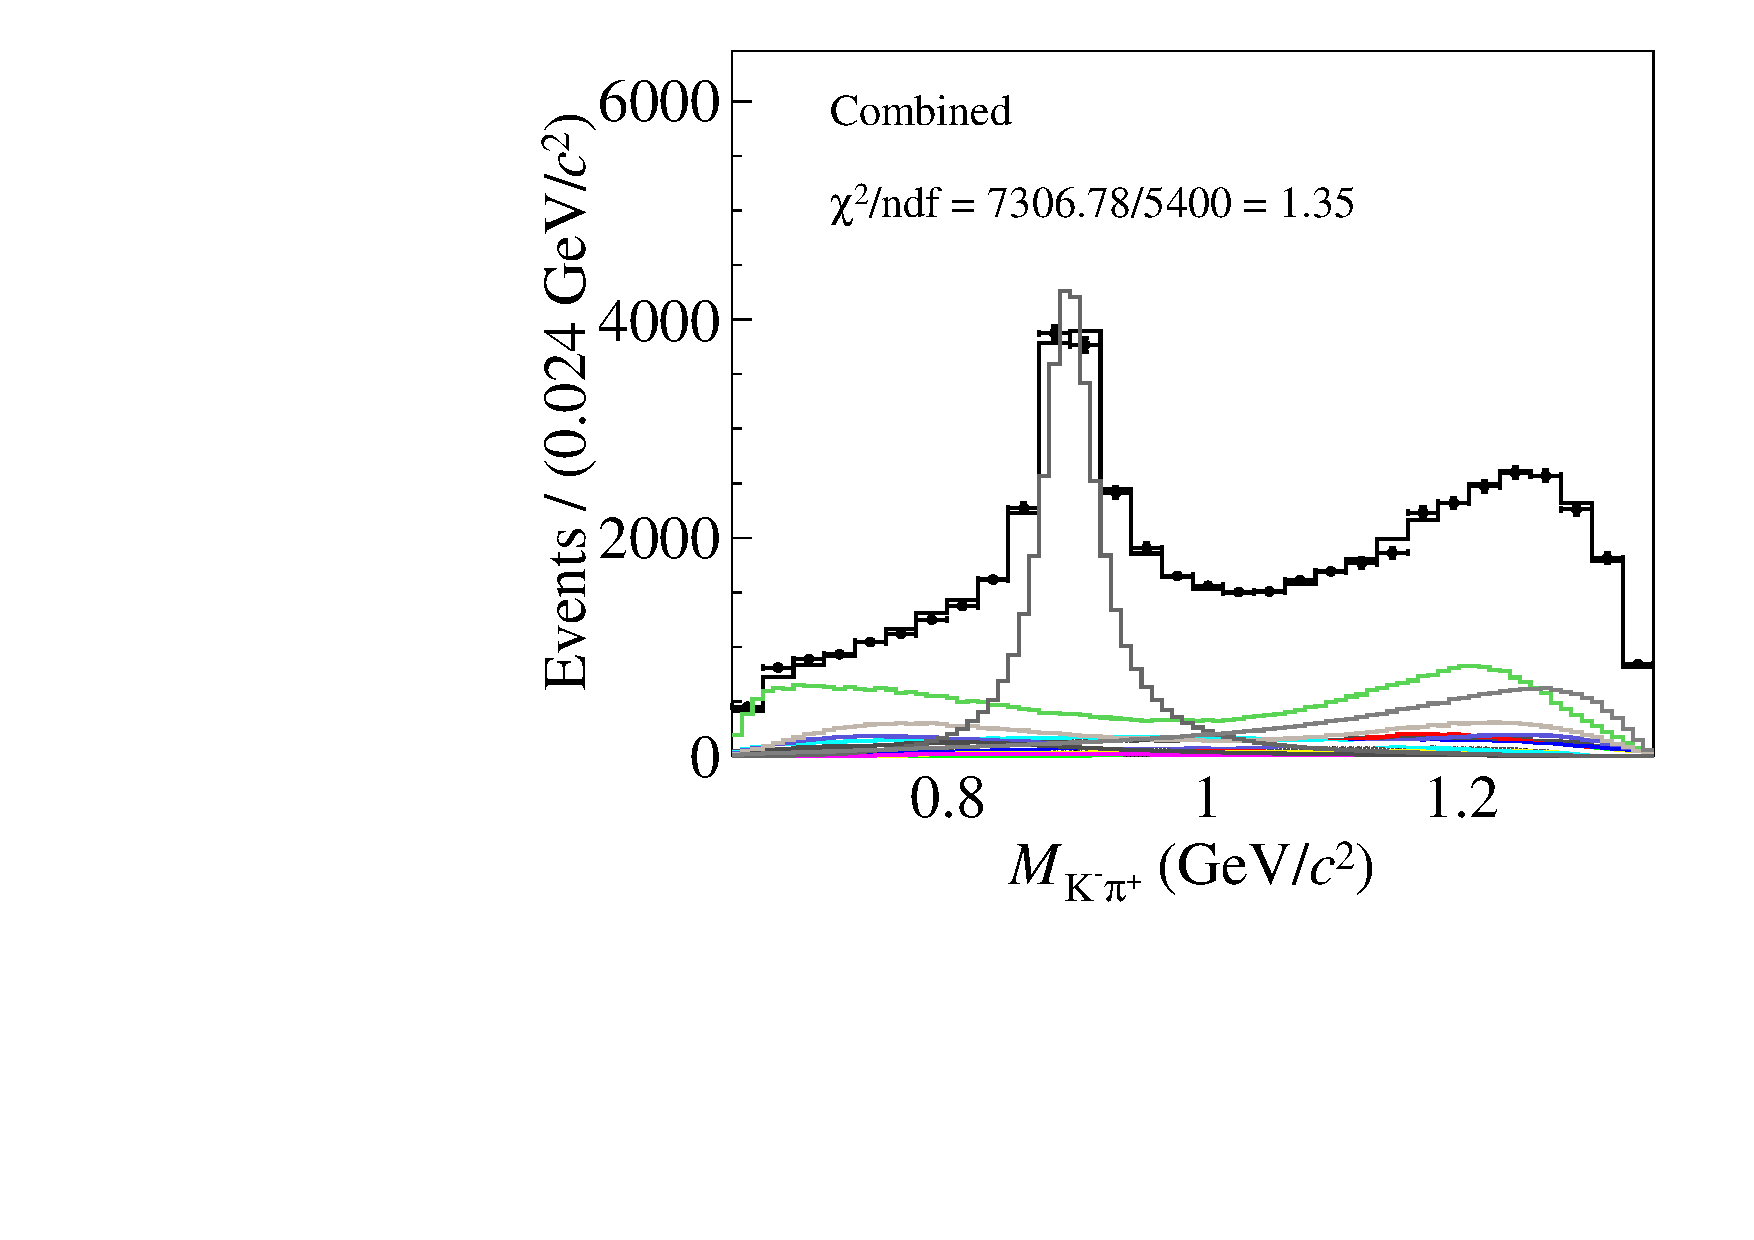
\includegraphics[width=0.32\textwidth]{figure/pwa_nominal/data_all_m_R_CD.pdf} \\
    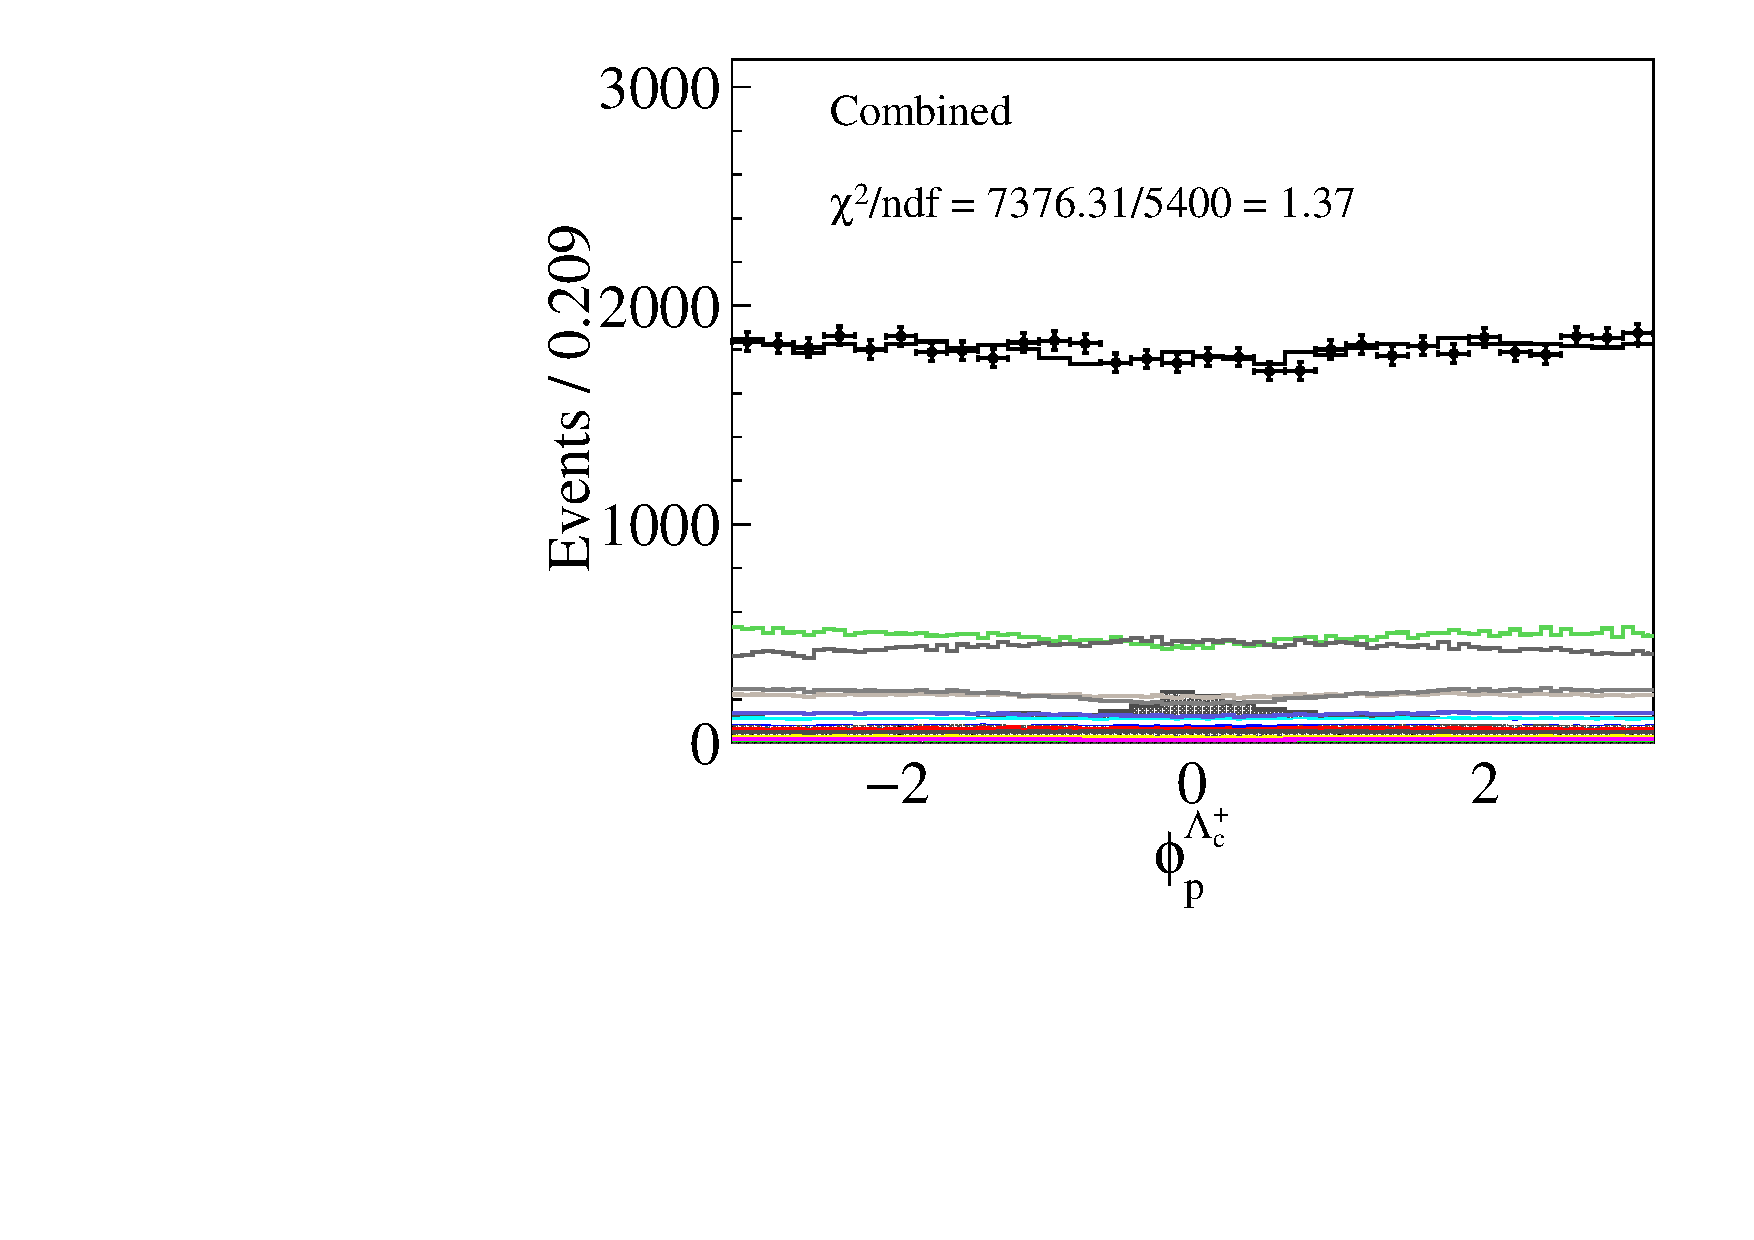
\includegraphics[width=0.32\textwidth]{figure/pwa_nominal/data_all_Lmdc_p_alpha.pdf}
    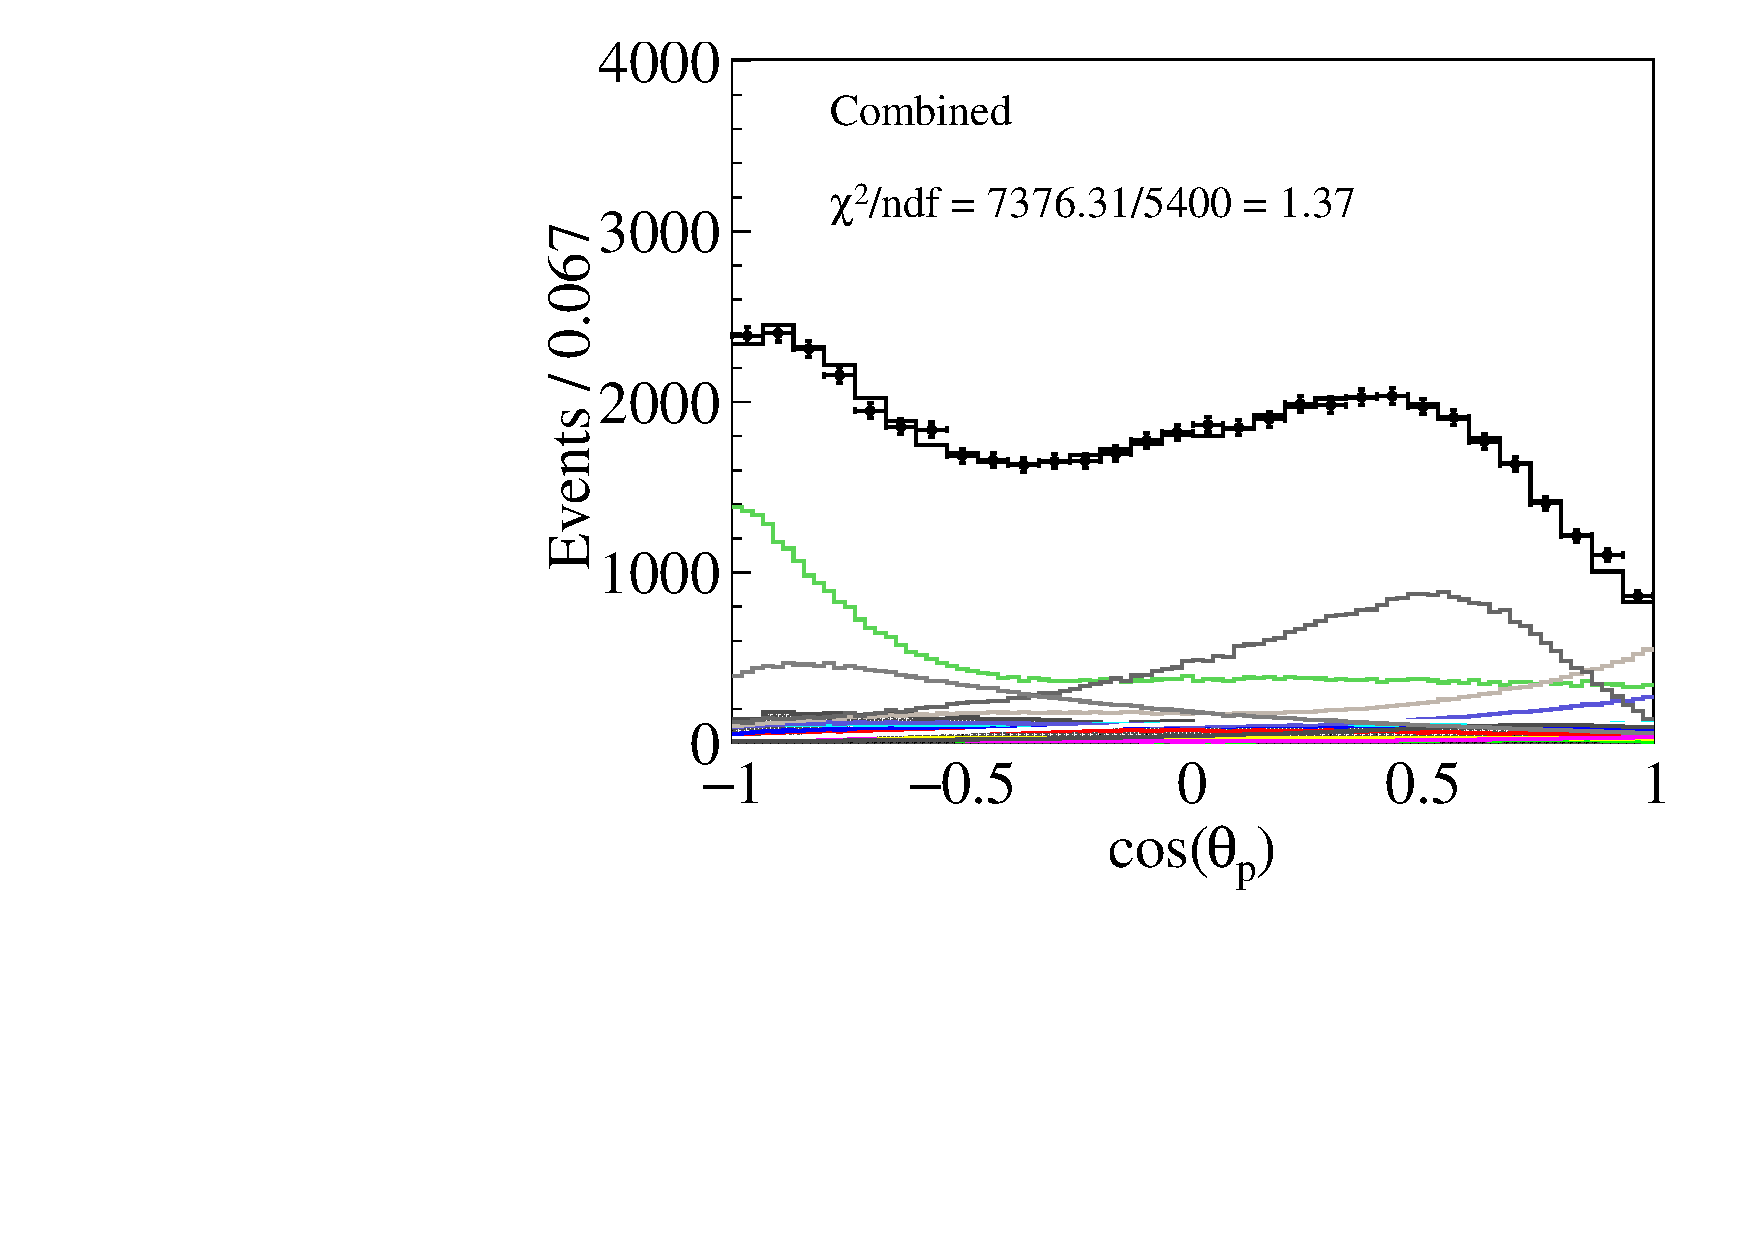
\includegraphics[width=0.32\textwidth]{figure/pwa_nominal/data_all_Lmdc_p_cos_beta.pdf}
    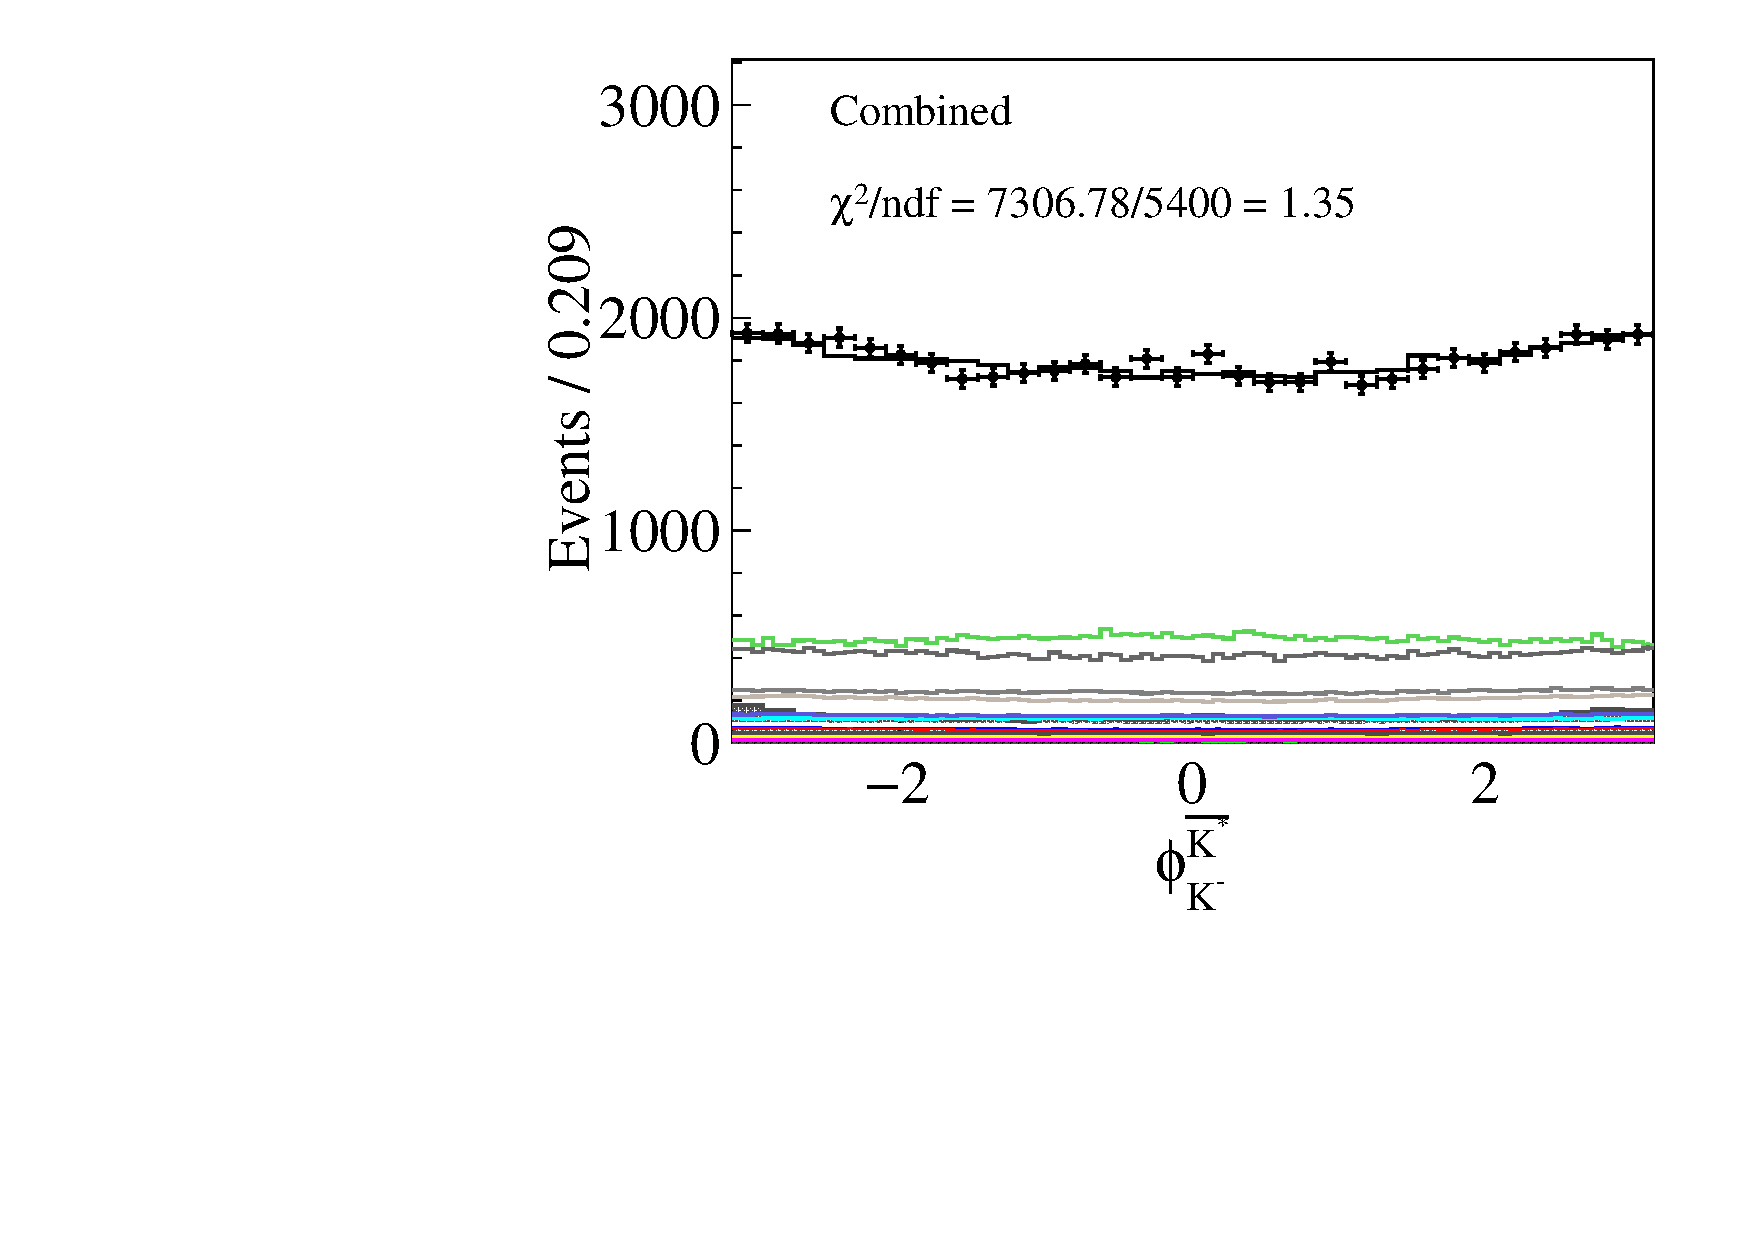
\includegraphics[width=0.32\textwidth]{figure/pwa_nominal/data_all_R_CD_k_alpha.pdf} \\
    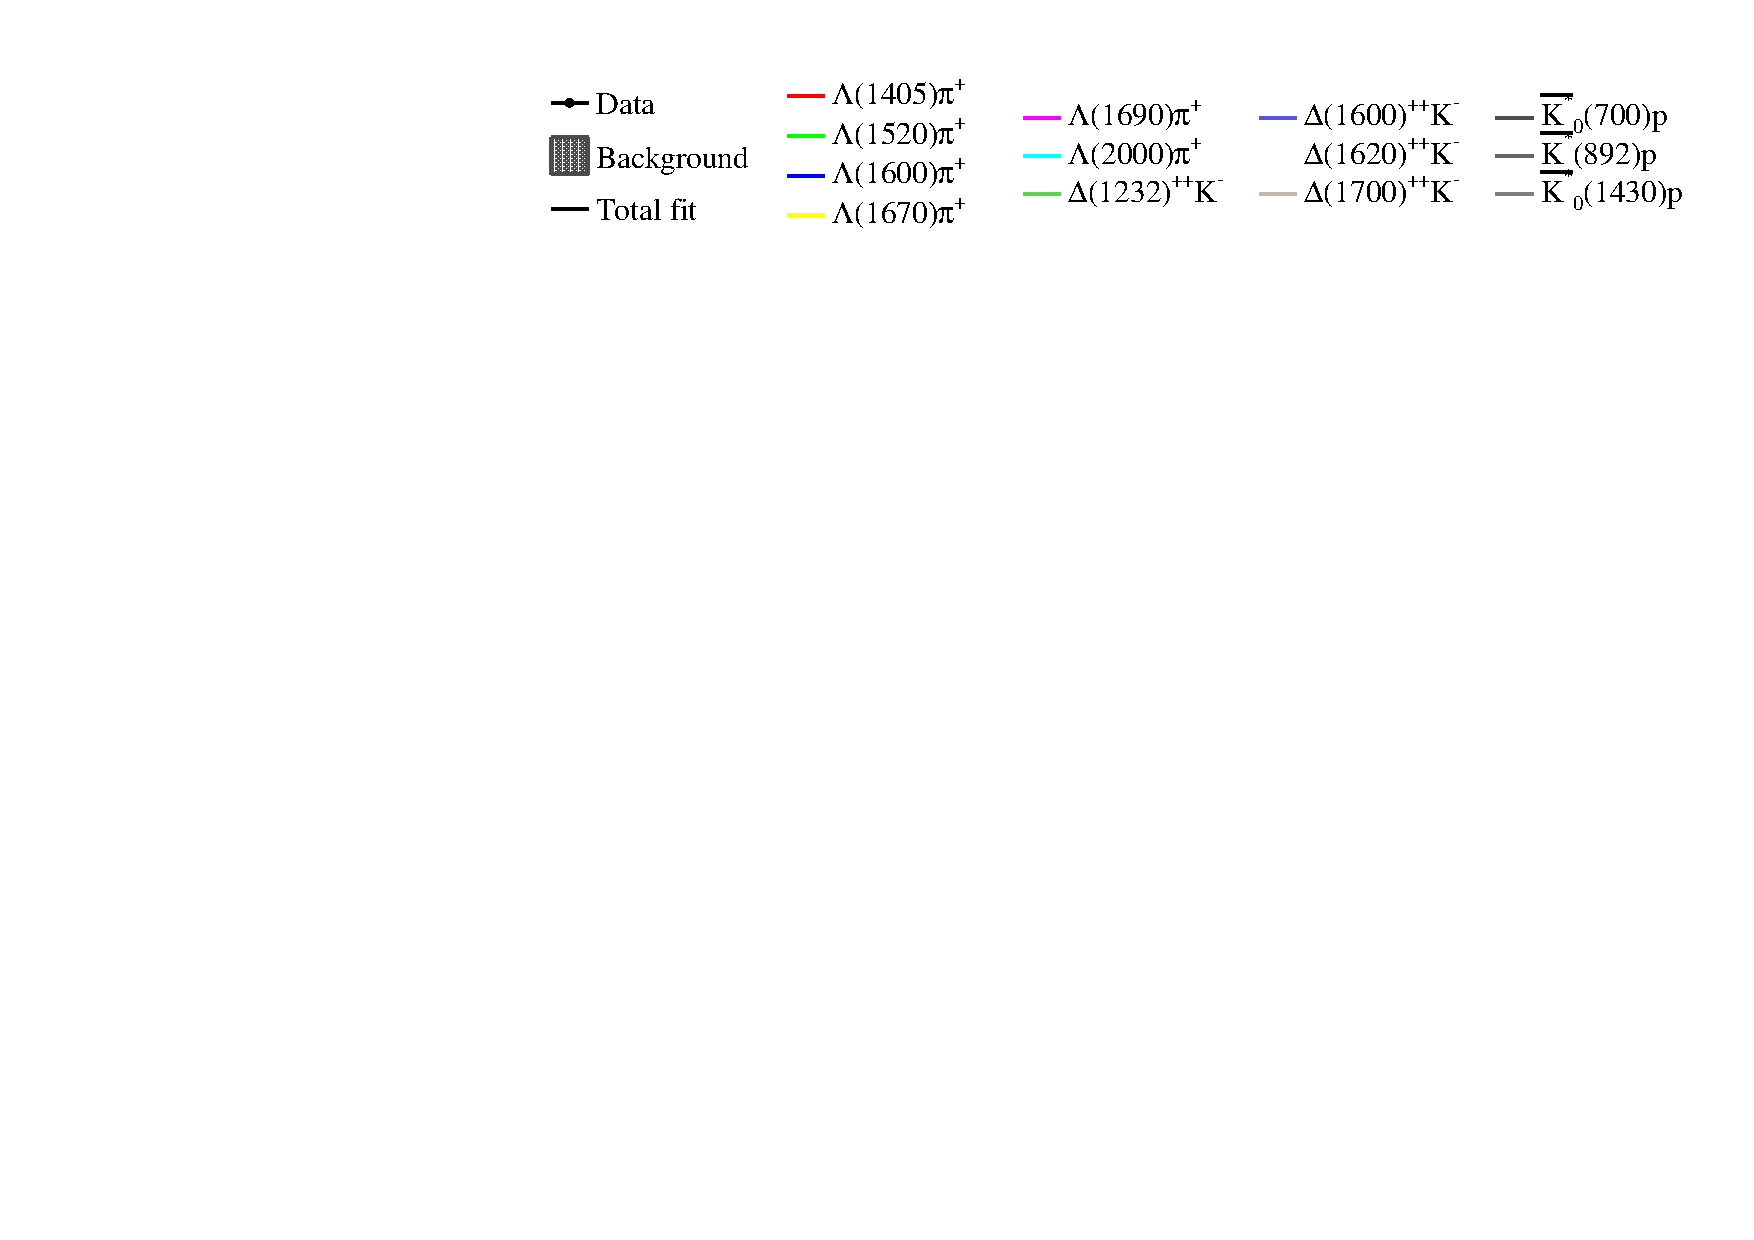
\includegraphics[width=0.80\textwidth]{figure/pwa_nominal/legend.pdf}

    \caption{Combined fit results of projected distributions of $M(pK^-)$, $M(p\pi^+)$, $M(K^-\pi^+)$ and helicity angle $\phi_{p}^{\lcp}$, $\cos(\theta_{p})$ and $\phi_{K^{-}}^{\bar{K^{*}}}$. }
\label{fig:pwa_nominal_comb}
\end{figure}

The projected invariant mass distributions from the fit results are shown in Figure~\ref{fig:pwa_fit_mass_0}-\ref{fig:pwa_fit_mass_1} for each energy points. As the parameters of $\lcp$ decay are shared among all energy points, the fit fractions results are almost same with possible small difference due to the statistical fluctuations from the PHSP MC samples. The fit fractions of each component and the interference part are shown in Table~\ref{tab:ff_s6} for $\sqrt{s} = 4.682\gev/c^2$. The total FF is 114.53$\pm$4.67\%. Comparison of FF of each component at different energy points are listed in Table~\ref{tab:ff_full}.  The partial wave amplitudes ($g_{ls}^{\gamma^*}$) and derived $\alpha_0$ and $\Delta_0$ are shown in Table~\ref{tab:fit_polarization} for each energy point.

\begin{table}[h]
    \centering
    \caption{The difference for NLL and NDF between with and without each resonance state, the statistical significance values for each component in the nominal model.}
    \label{tab:nom_significance}
    \begin{tabular}{cccc}
        \hline\hline
    Resonance & $\Delta_{\rm NLL}$ & $\Delta_{\rm NDF}$ & Significance \\\hline
    $\Lambda(1405)$ & 99.4 & 4 & 13.6$\sigma$ \\
    $\Lambda(1520)$ & 74.7 & 4 & 11.6$\sigma$ \\
    $\Lambda(1600)$ & 26.0 & 4 & 6.4$\sigma$ \\
    $\Lambda(1670)$ & 92.0 & 4 & 13.0$\sigma$ \\
    $\Lambda(1690)$ & 28.4 & 4 & 6.8$\sigma$ \\
    $\Lambda(2000)$ & 244.1 & 4 & 21.7$\sigma$ \\
    $\Delta(1232)^{++}$ & 517.6 & 4 & 31.9$\sigma$ \\
    $\Delta(1600)^{++}$ & 32.6 & 4 & 7.3$\sigma$ \\
    $\Delta(1620)^{++}$ & 21.4 & 4 & 5.7$\sigma$ \\
    $\Delta(1700)^{++}$ & 47.1 & 4 & 9.0$\sigma$ \\
    $\overline{K}^{*}_{0}(700)$ & 32.3 & 4 & 7.3$\sigma$ \\
    $\overline{K}^{*}(892)$ & 1293.0 & 8 & $>30\sigma$ \\
    $\overline{K}^{*}_{0}(1430)$ & 59.3 & 4 & 10.3$\sigma$ \\
    \hline\hline
    \end{tabular}
\end{table}

\begin{figure}[htbp]\centering
    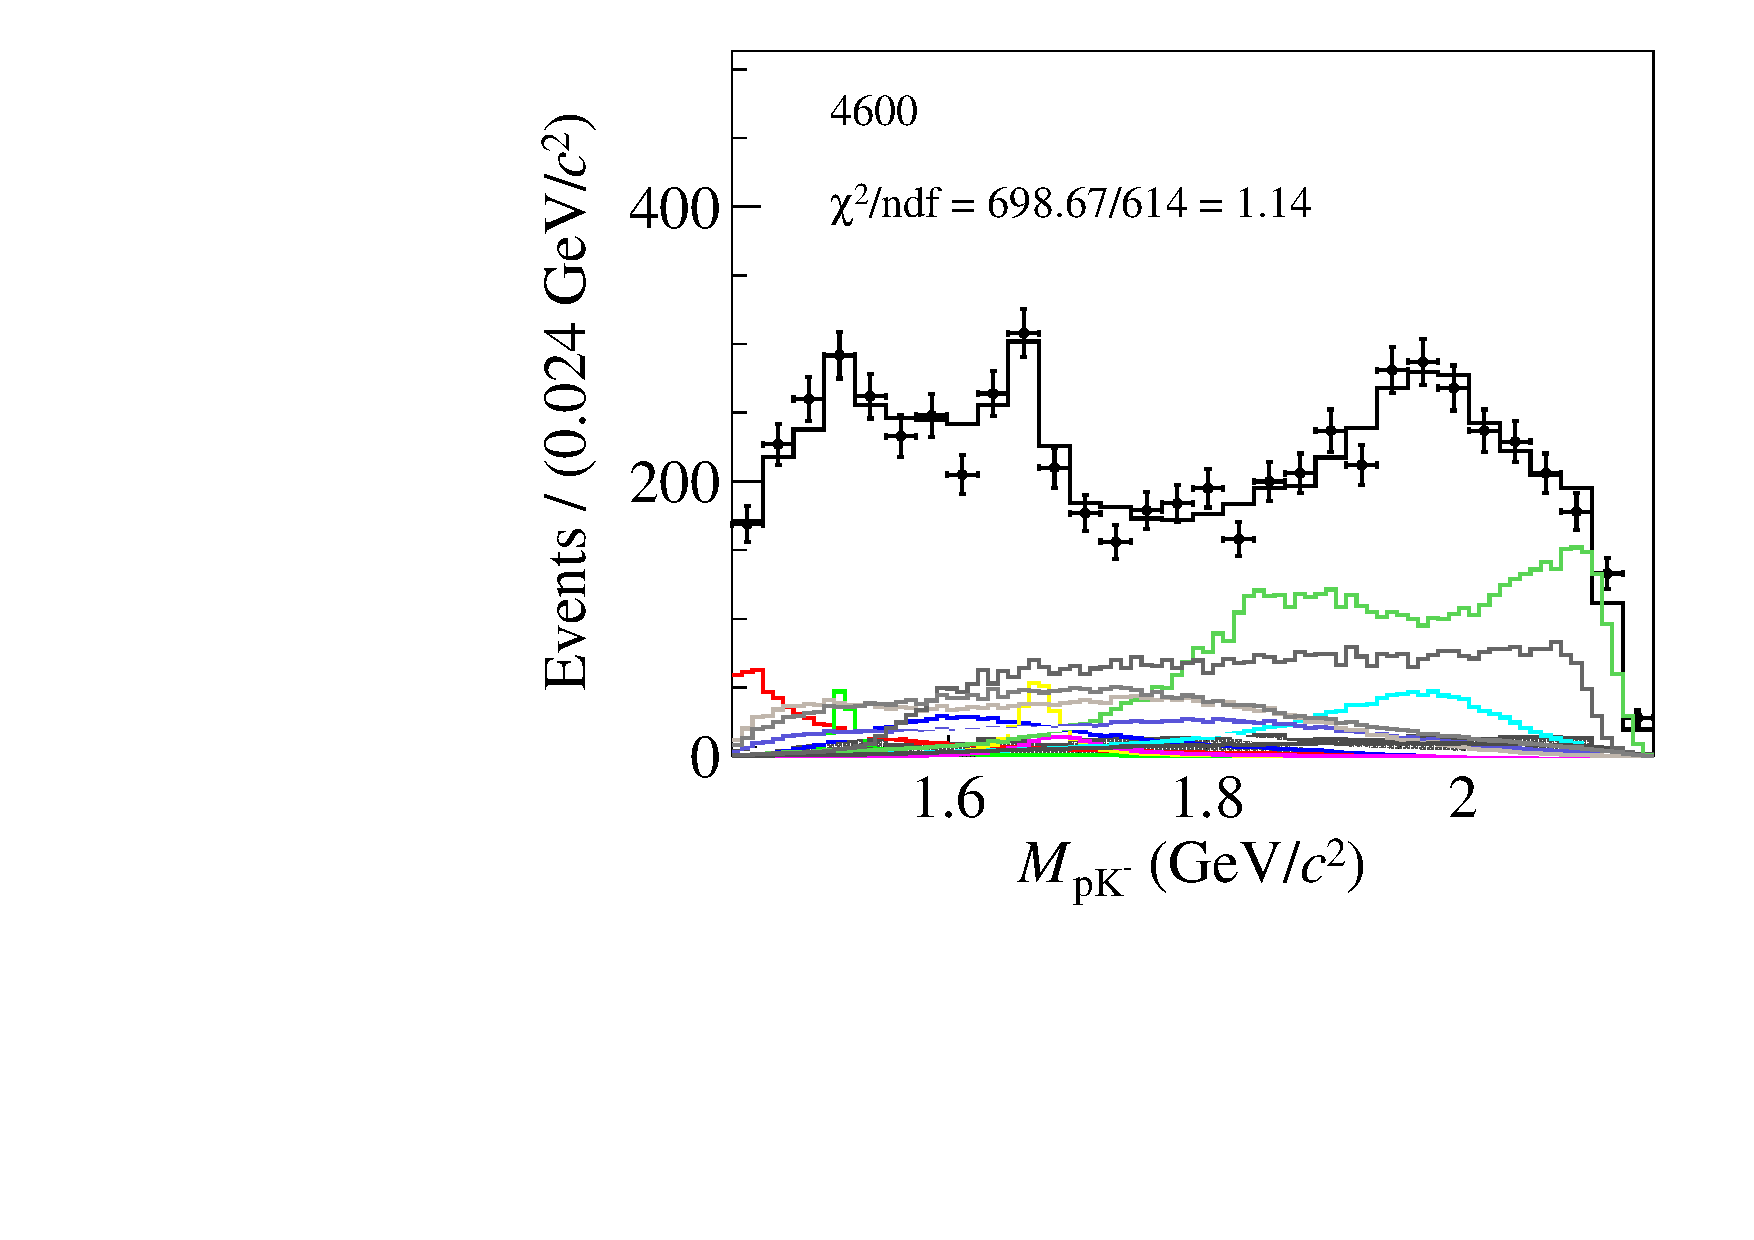
\includegraphics[width=0.24\textwidth]{figure/pwa_nominal/s0_m_R_BC.pdf}
    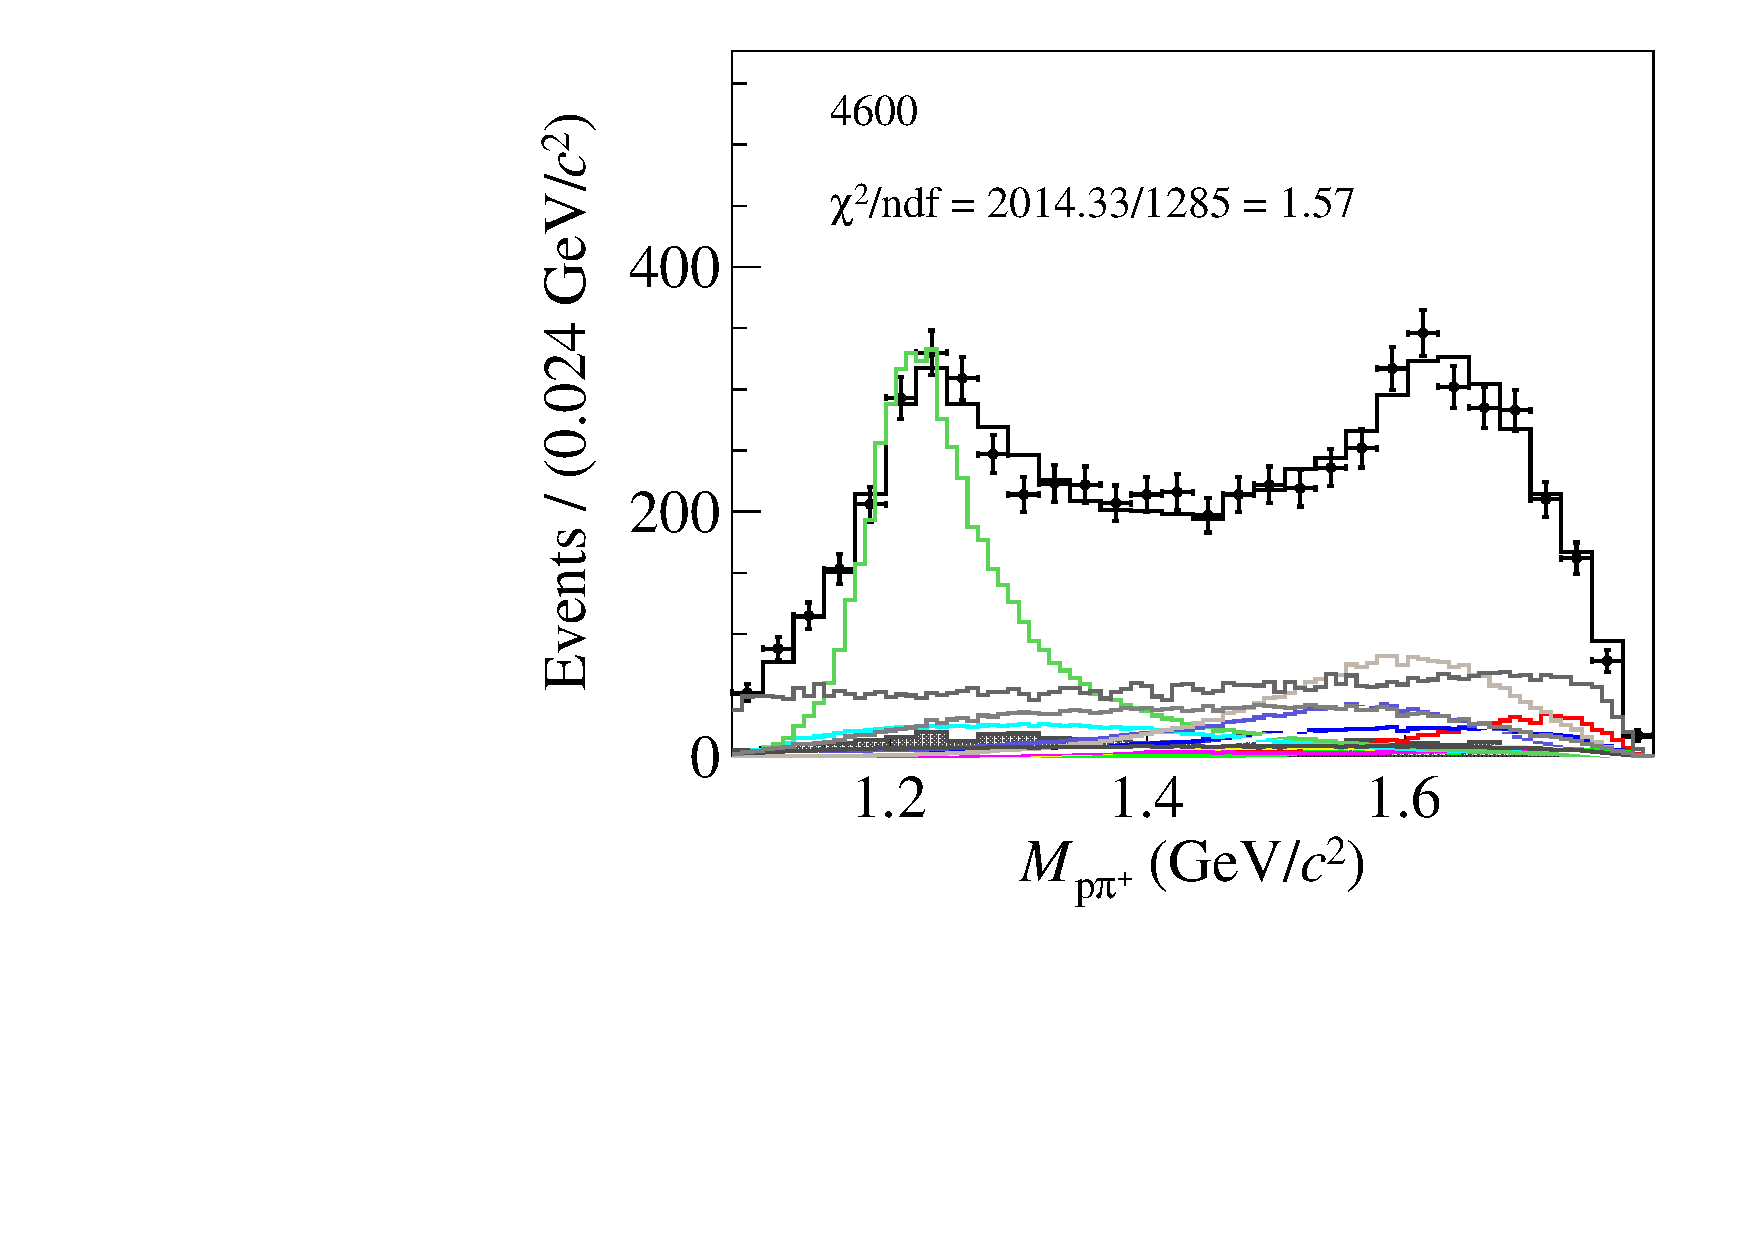
\includegraphics[width=0.24\textwidth]{figure/pwa_nominal/s0_m_R_BD.pdf}
    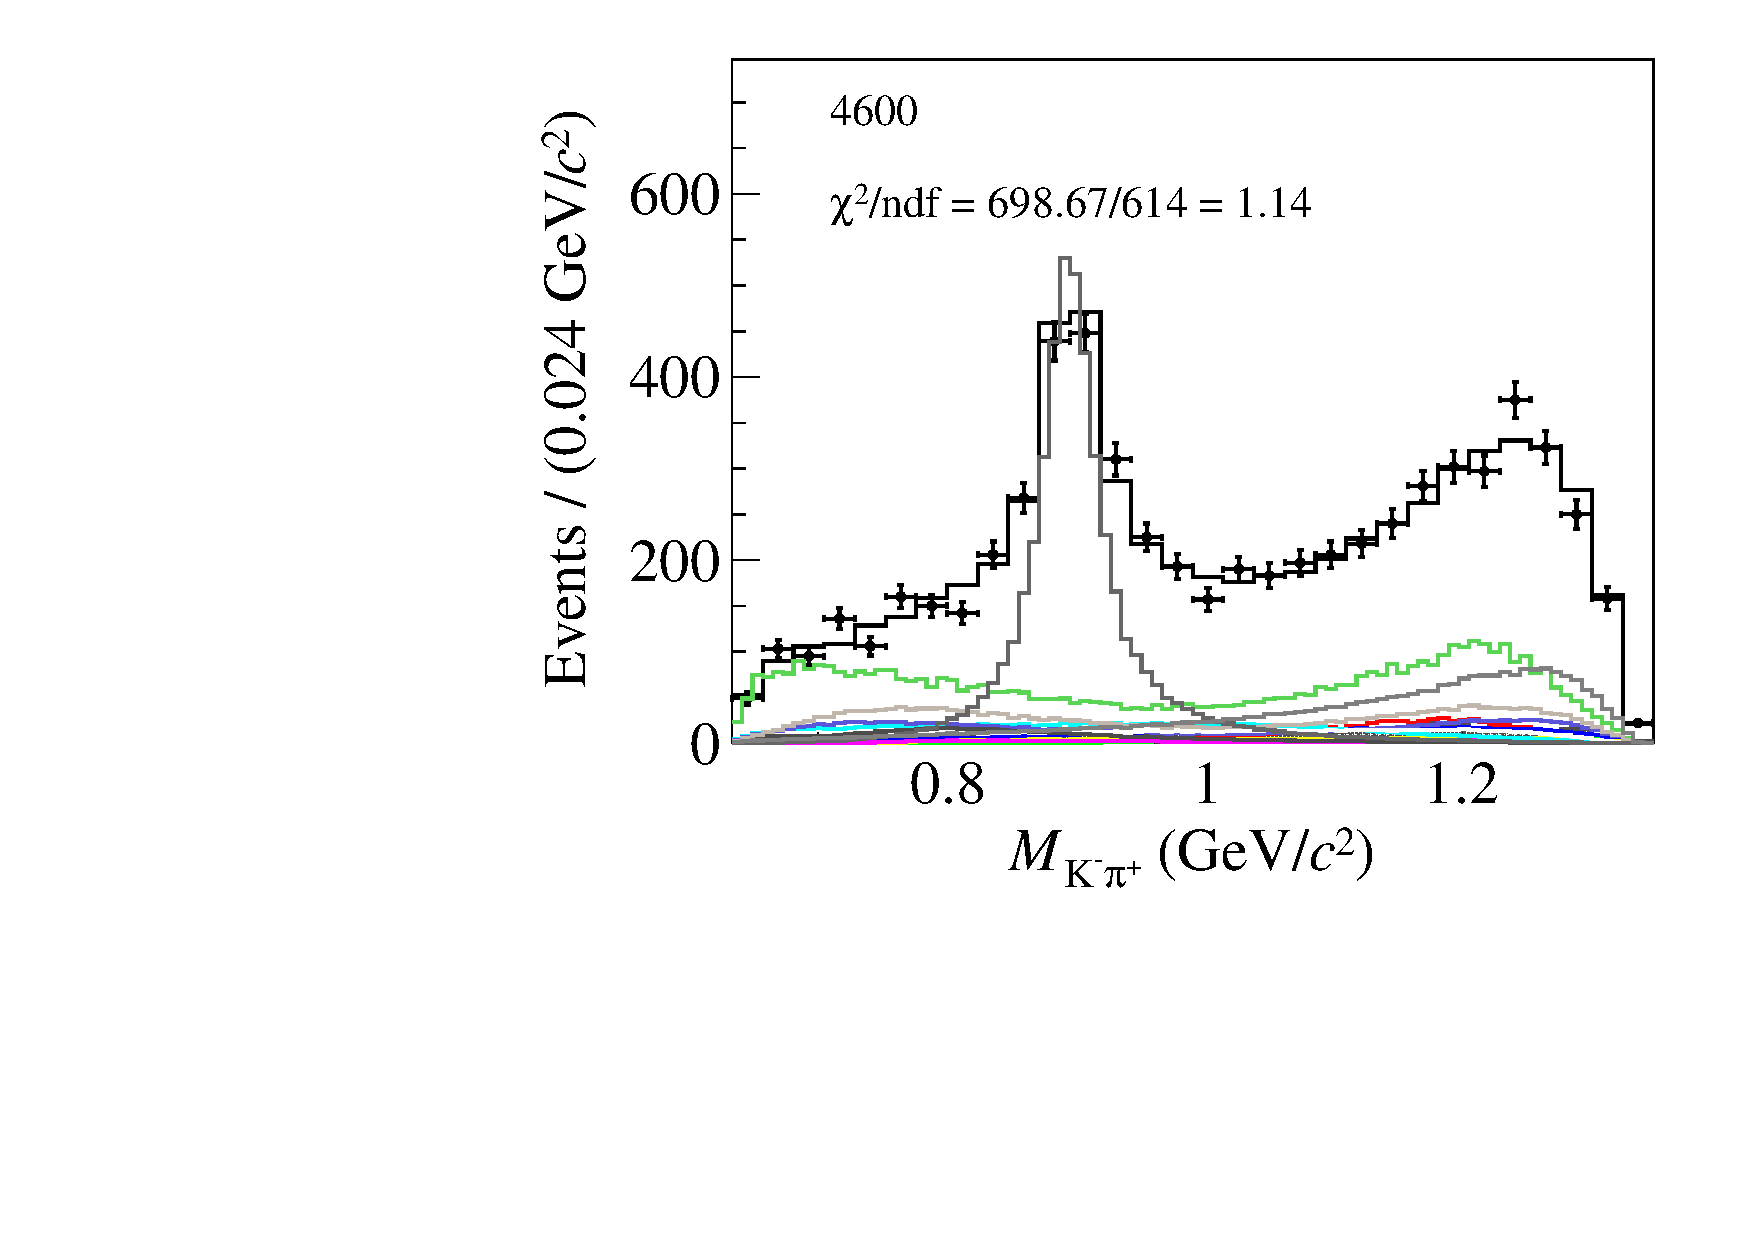
\includegraphics[width=0.24\textwidth]{figure/pwa_nominal/s0_m_R_CD.pdf}
    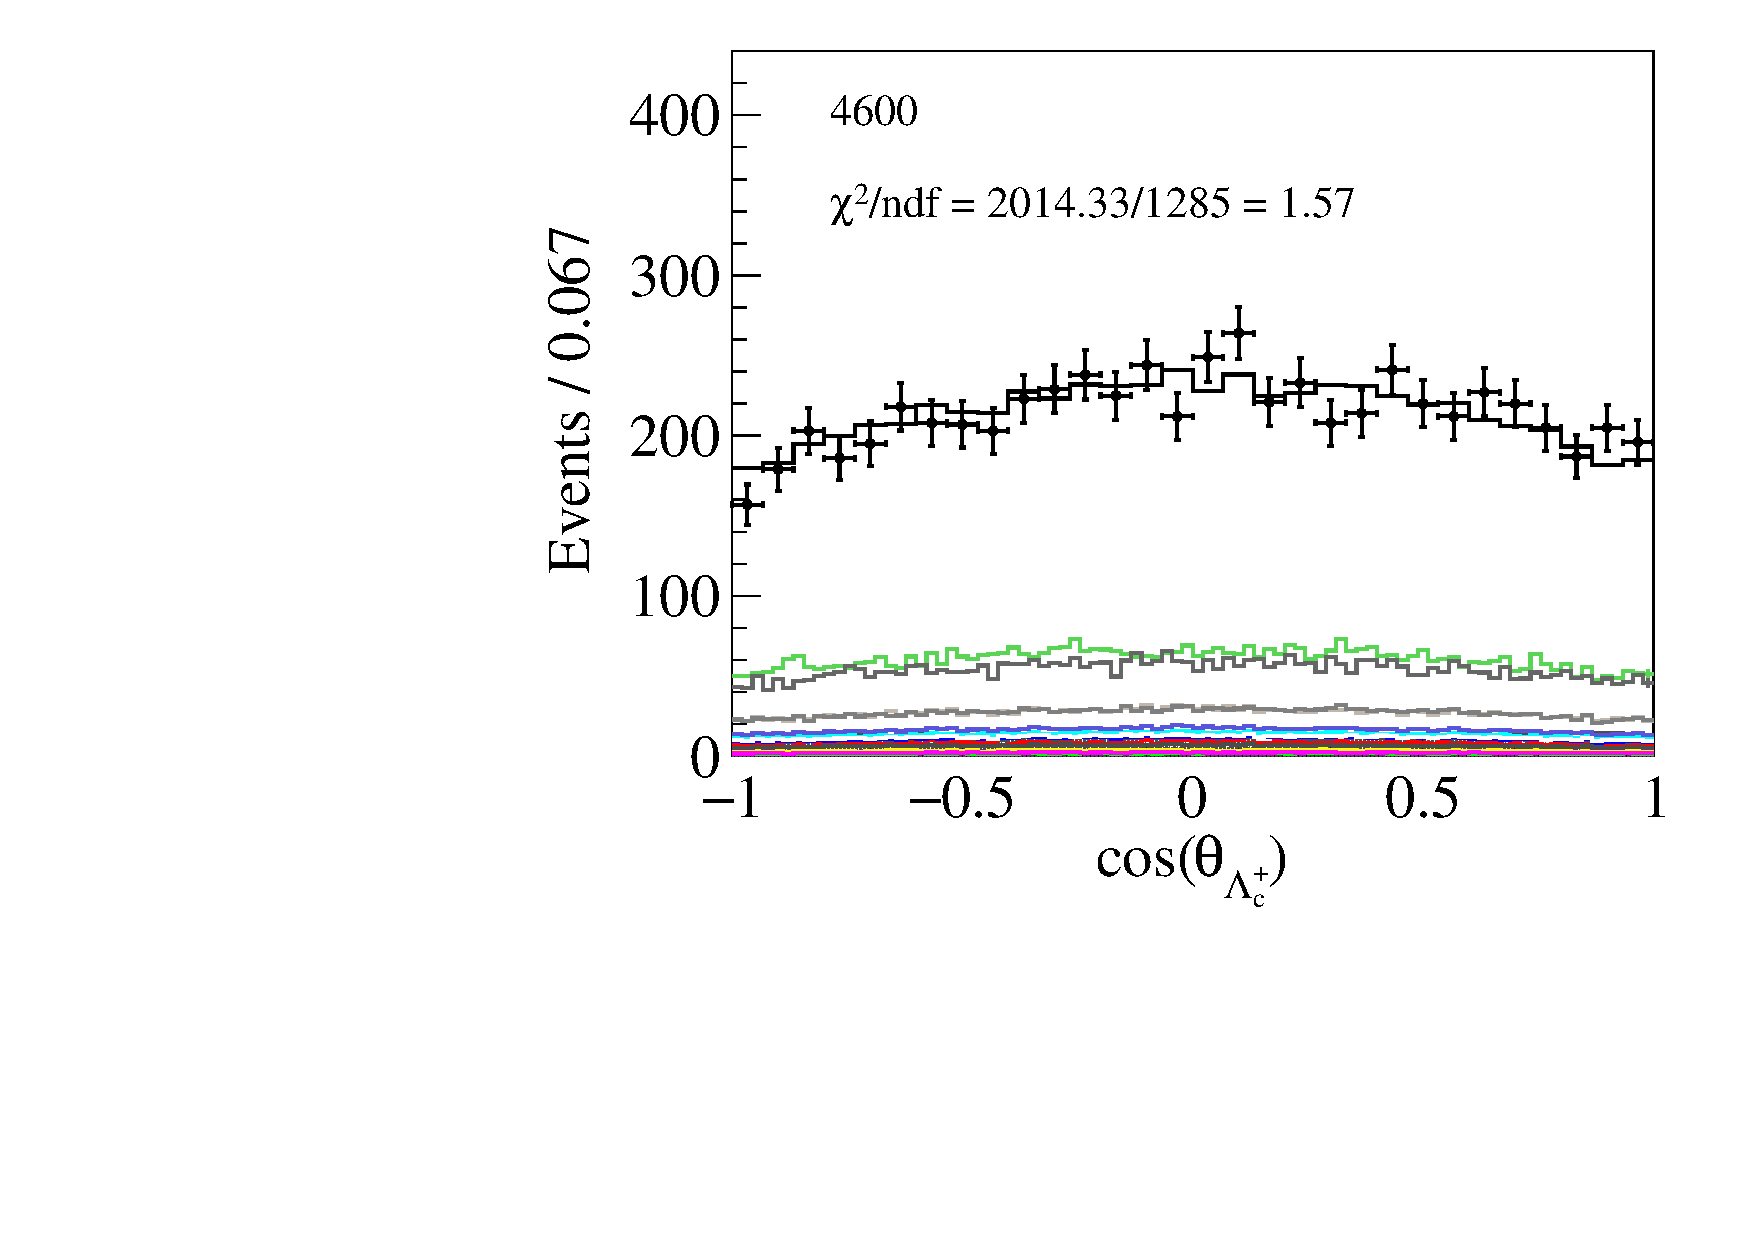
\includegraphics[width=0.24\textwidth]{figure/pwa_nominal/s0_epemDSID_Lmdc_cos_beta.pdf} \\
    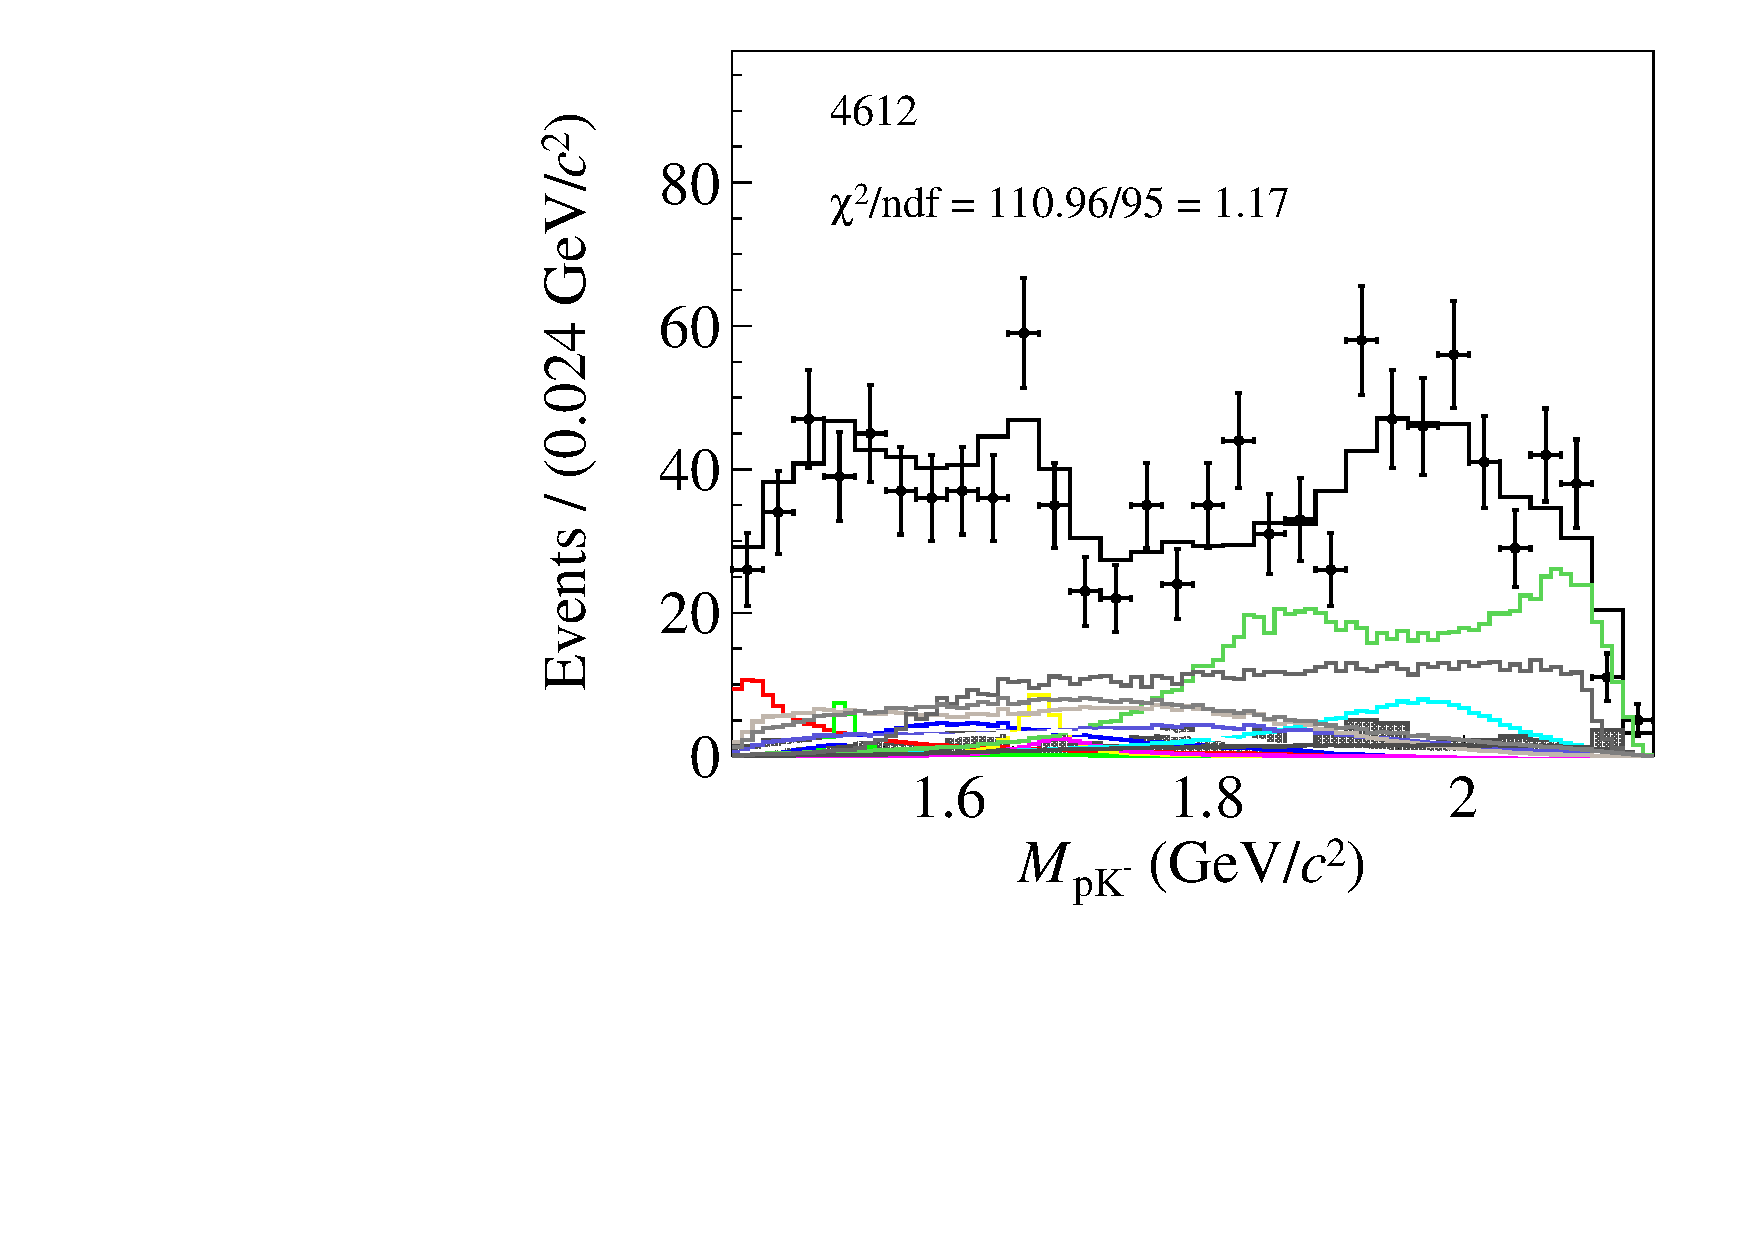
\includegraphics[width=0.24\textwidth]{figure/pwa_nominal/s1_m_R_BC.pdf}
    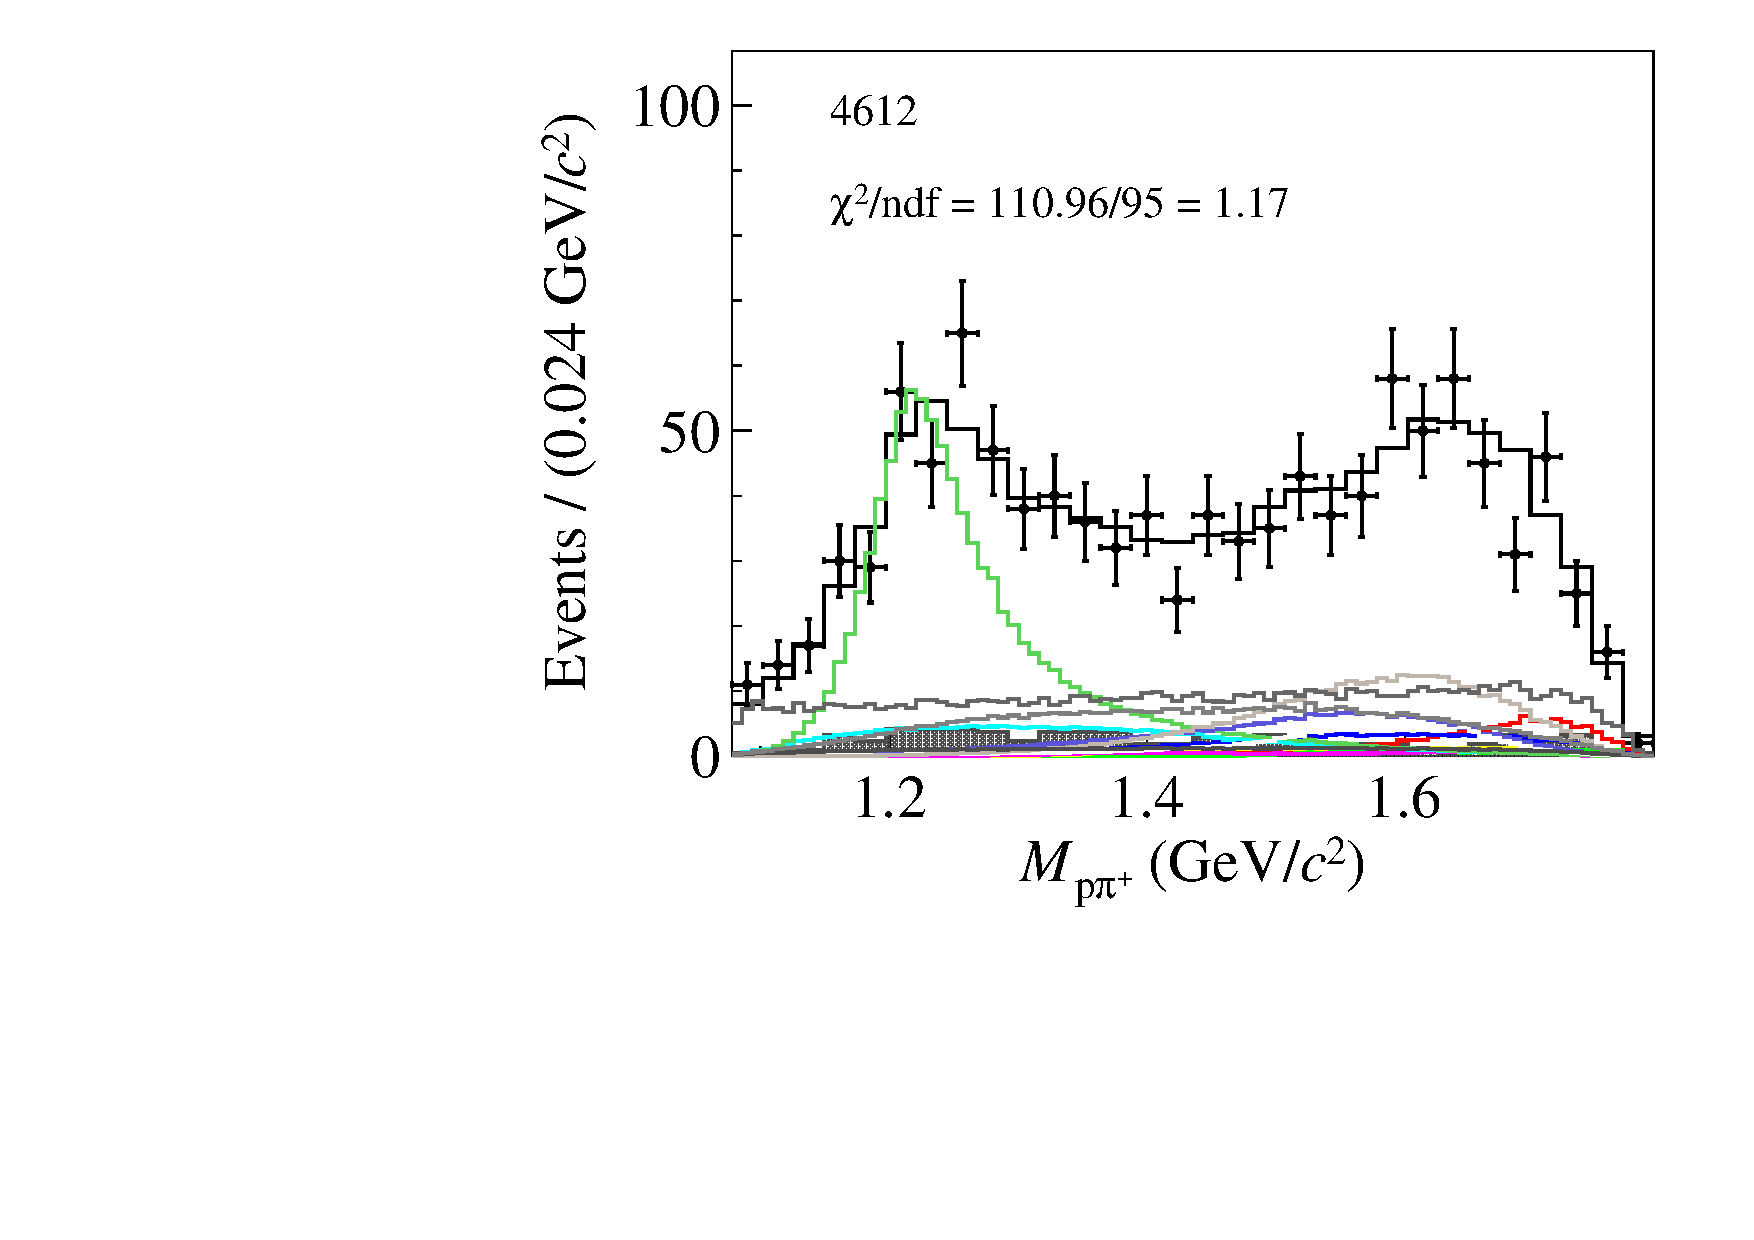
\includegraphics[width=0.24\textwidth]{figure/pwa_nominal/s1_m_R_BD.pdf}
    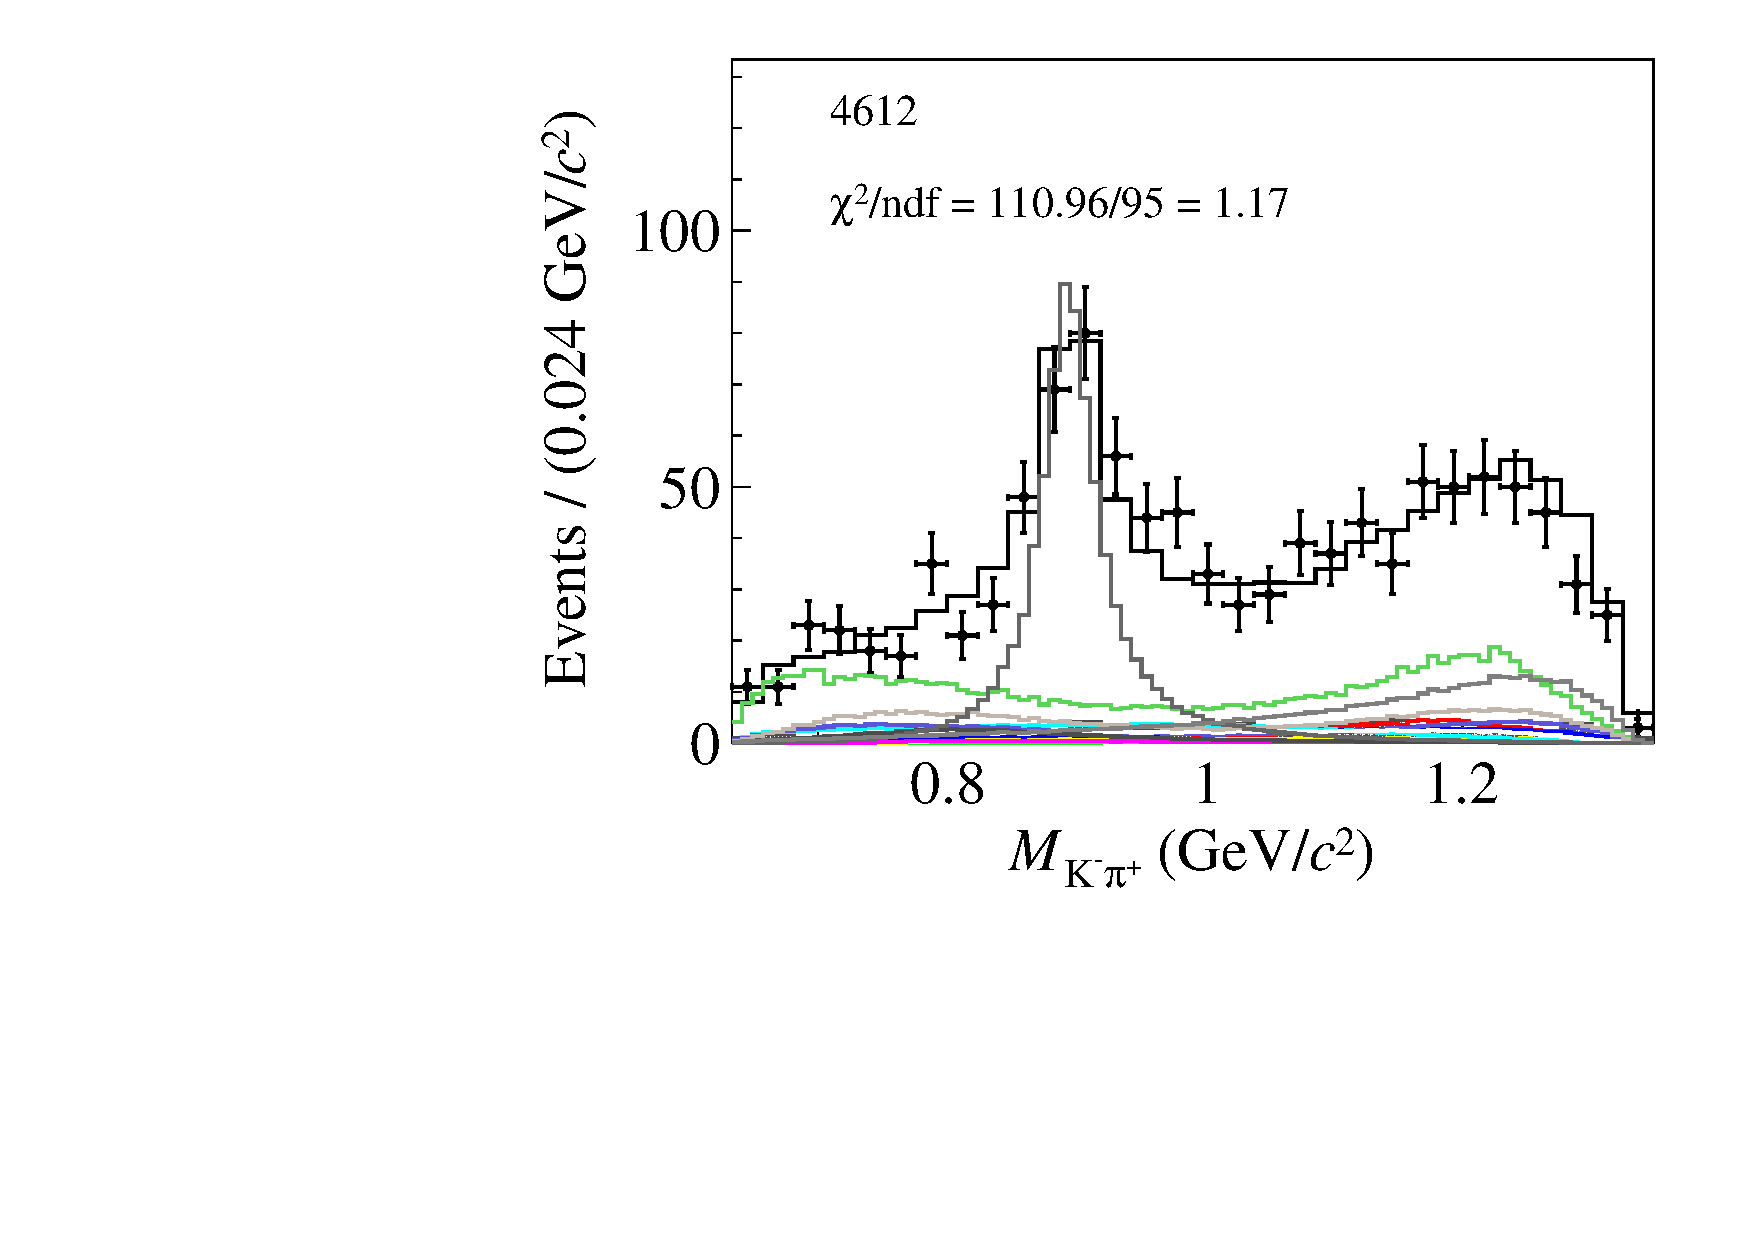
\includegraphics[width=0.24\textwidth]{figure/pwa_nominal/s1_m_R_CD.pdf}
    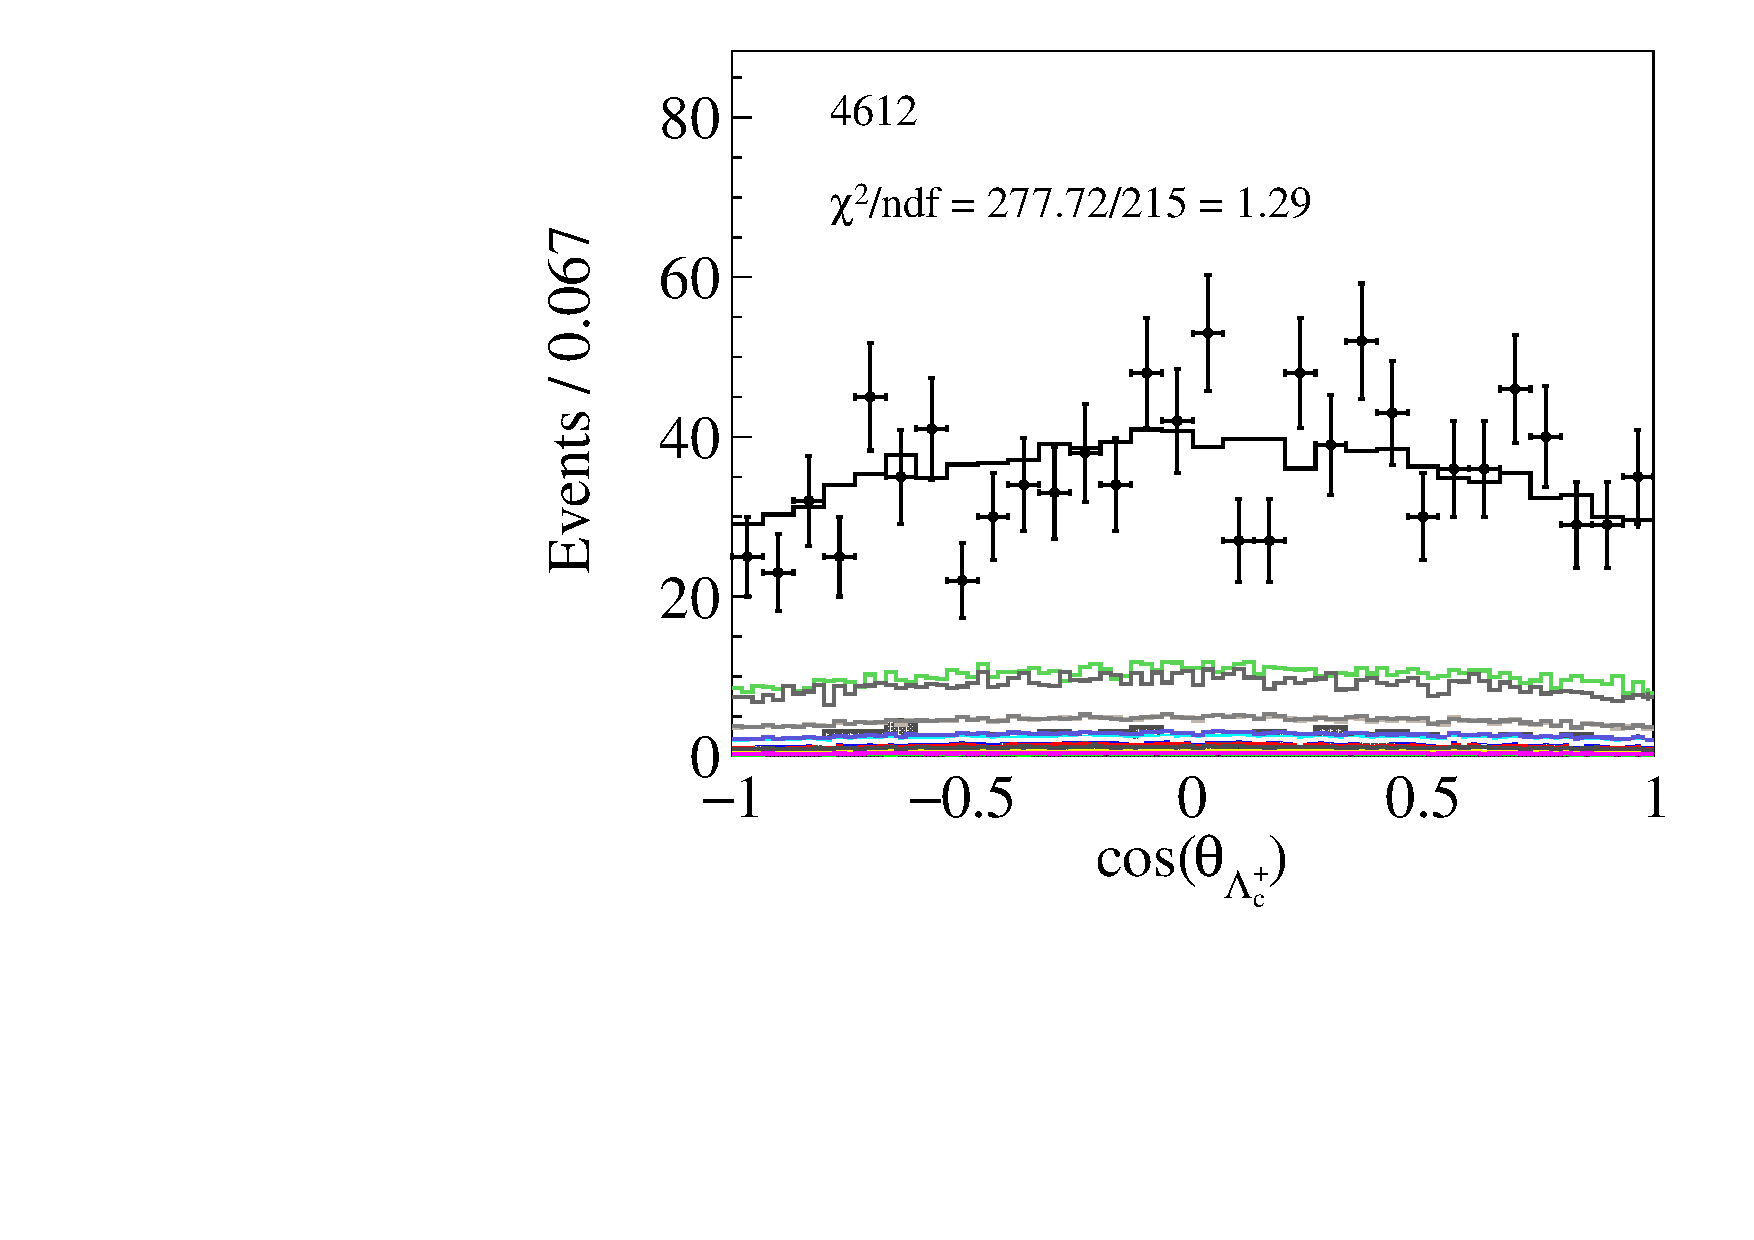
\includegraphics[width=0.24\textwidth]{figure/pwa_nominal/s1_epemDSID_Lmdc_cos_beta.pdf} \\
    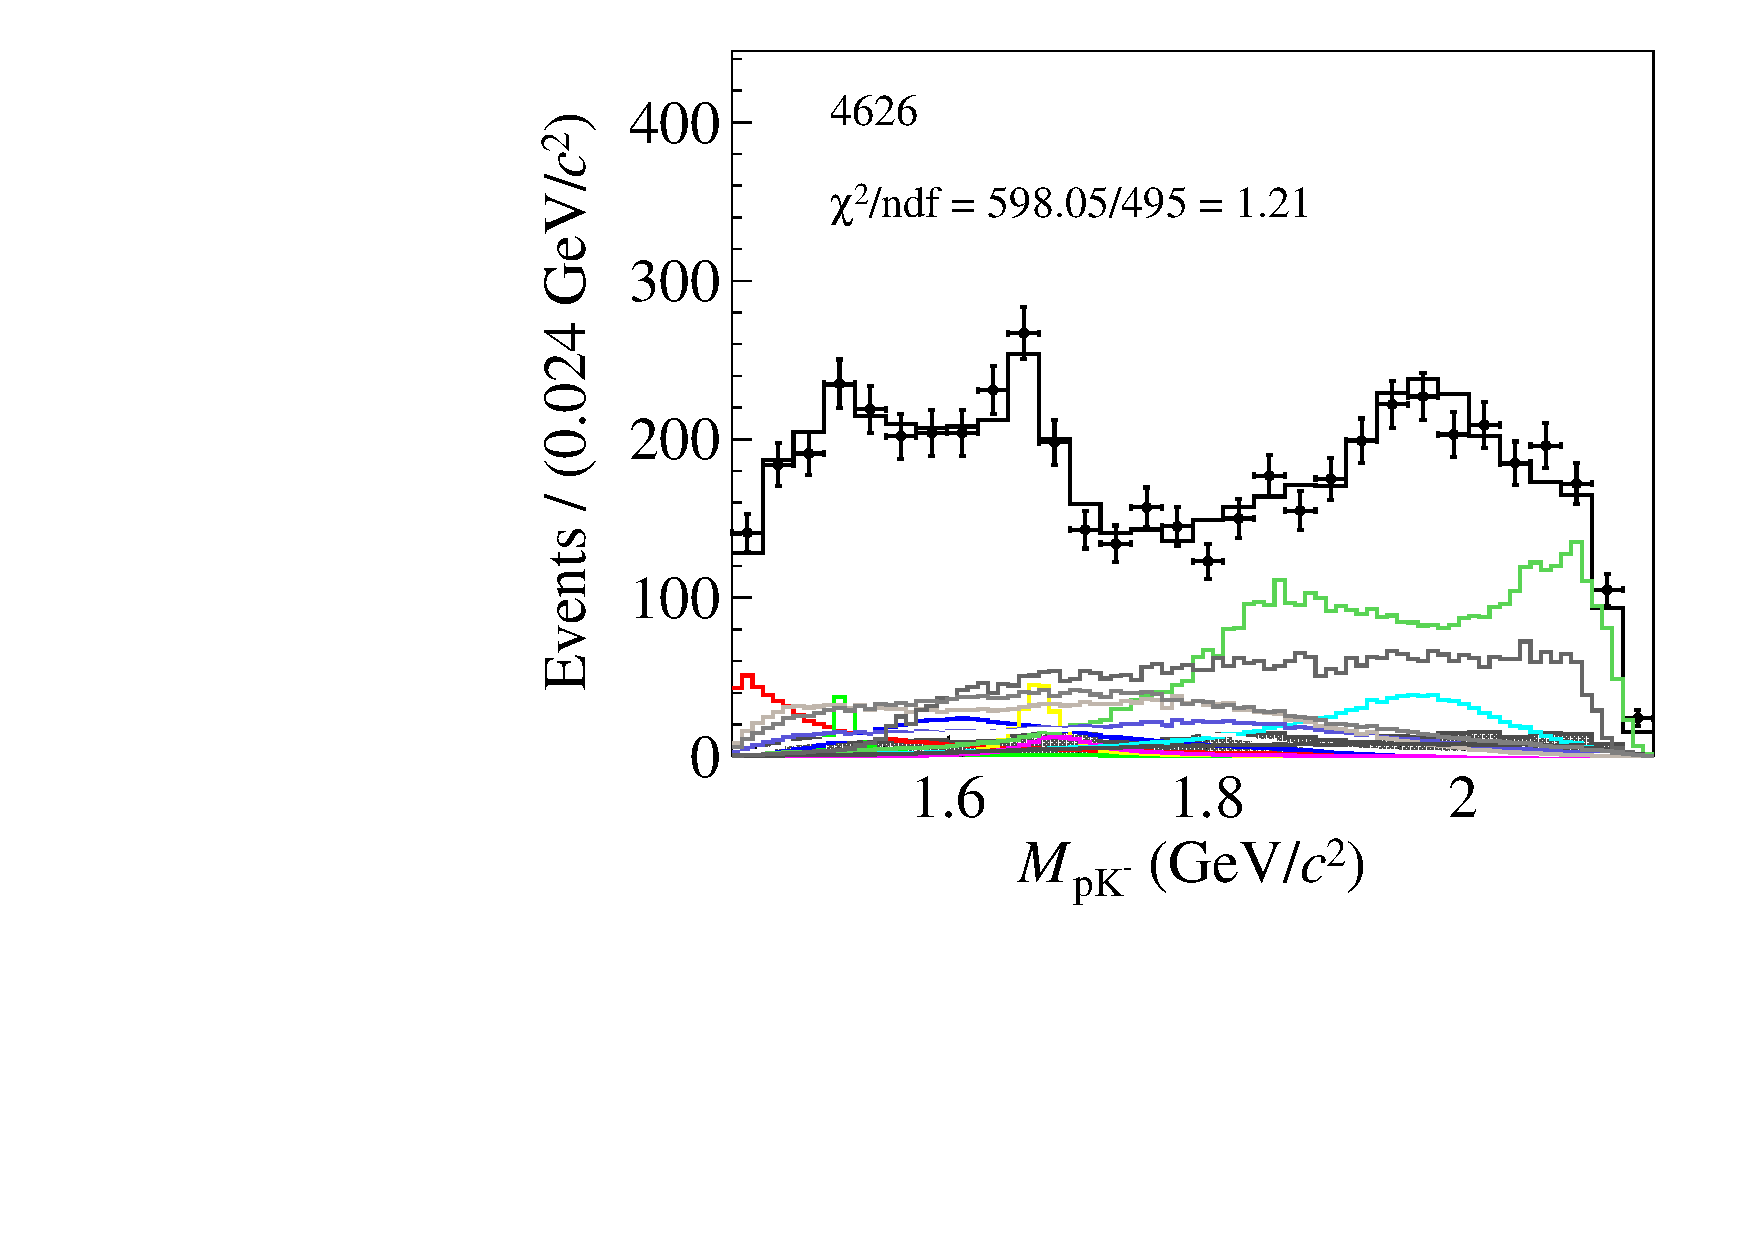
\includegraphics[width=0.24\textwidth]{figure/pwa_nominal/s2_m_R_BC.pdf}
    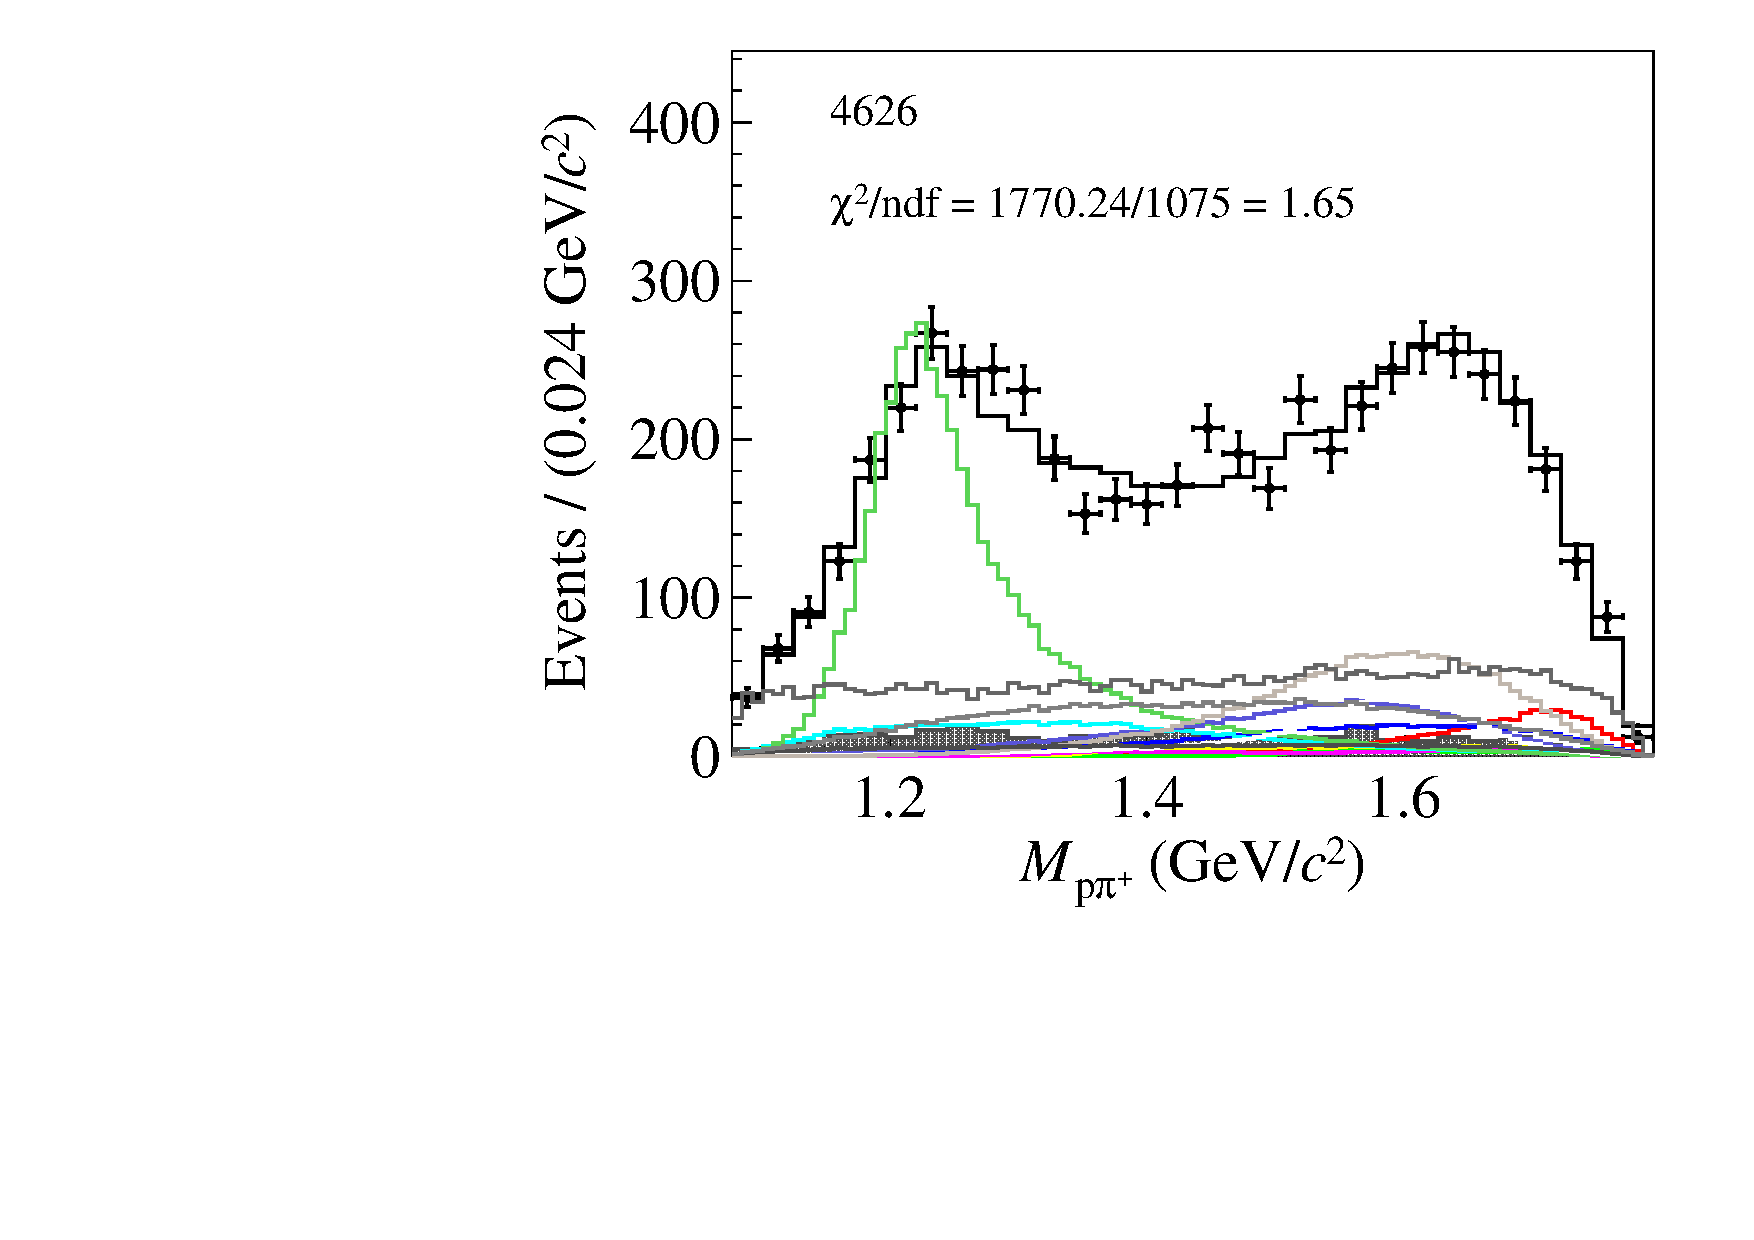
\includegraphics[width=0.24\textwidth]{figure/pwa_nominal/s2_m_R_BD.pdf}
    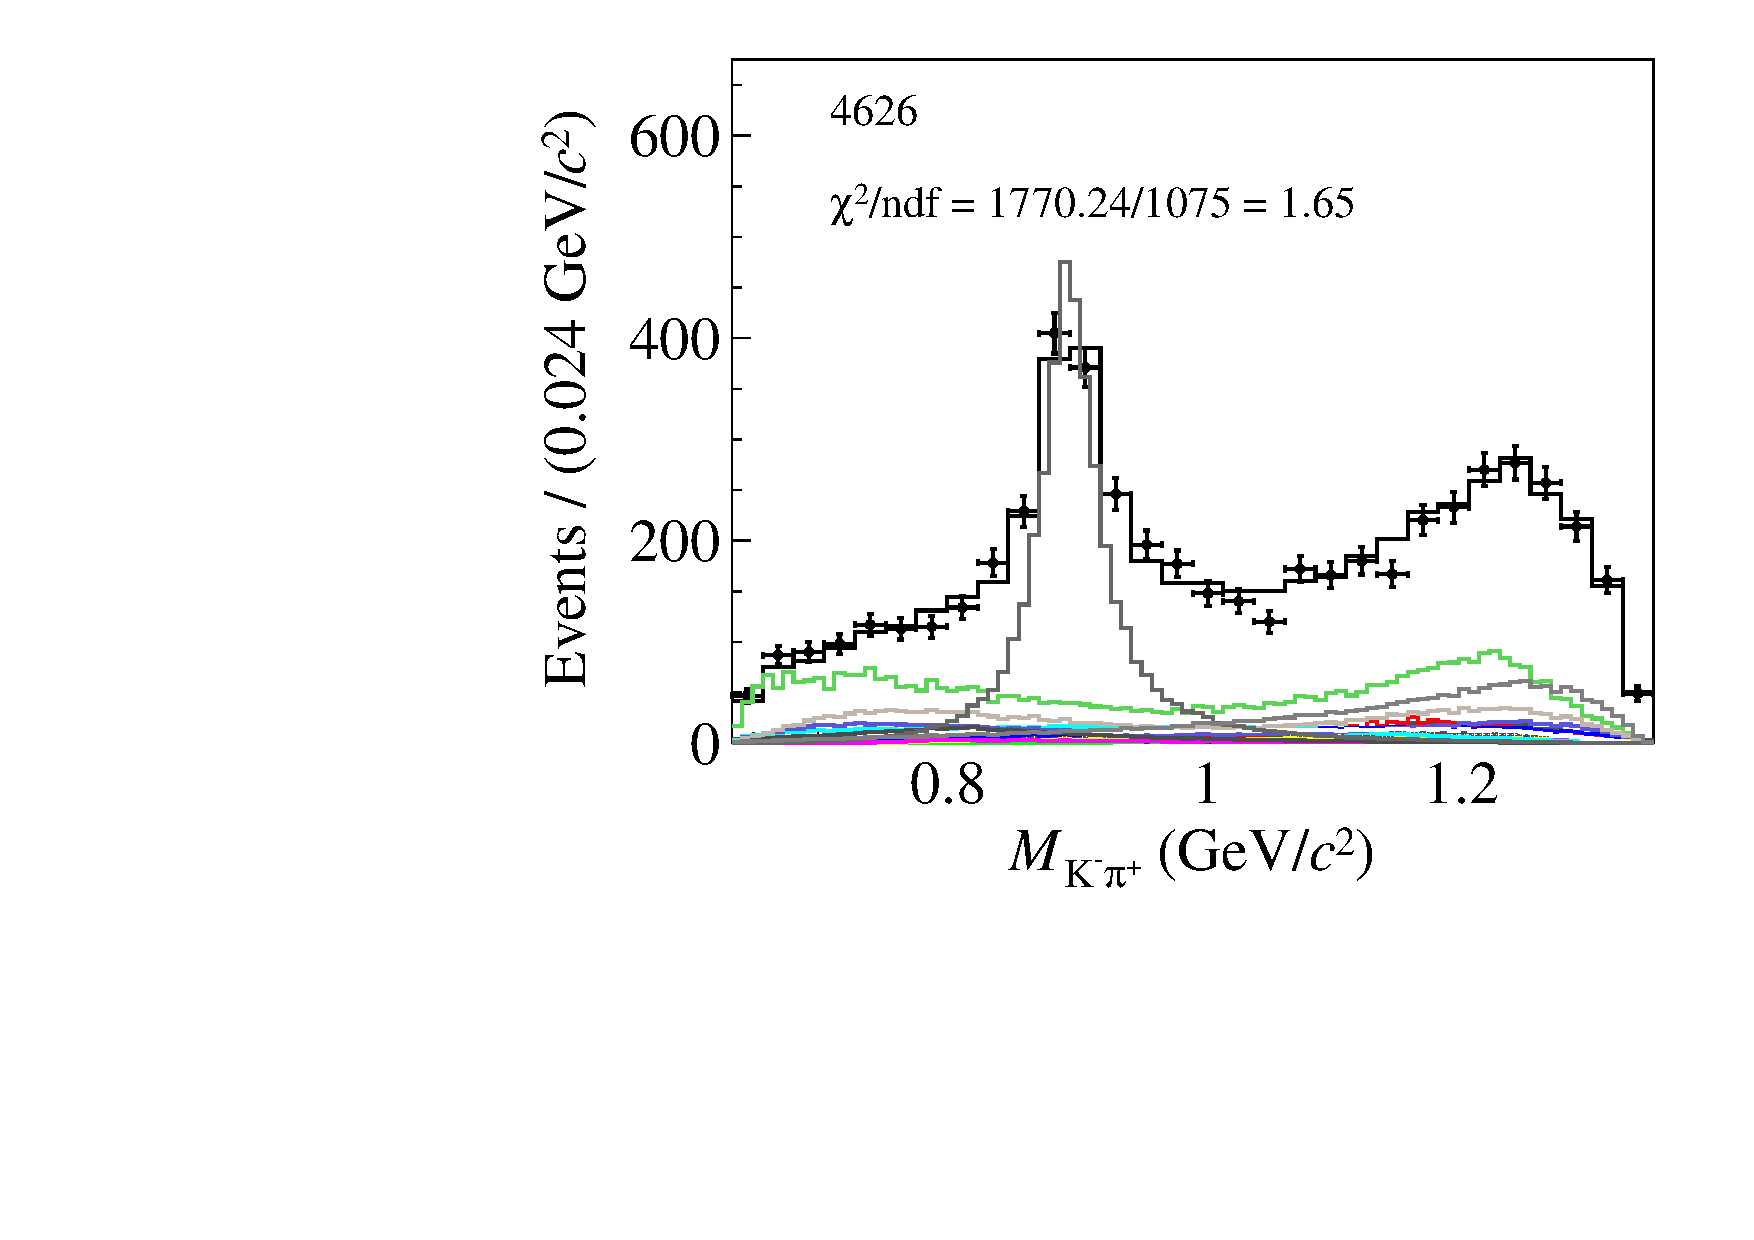
\includegraphics[width=0.24\textwidth]{figure/pwa_nominal/s2_m_R_CD.pdf}
    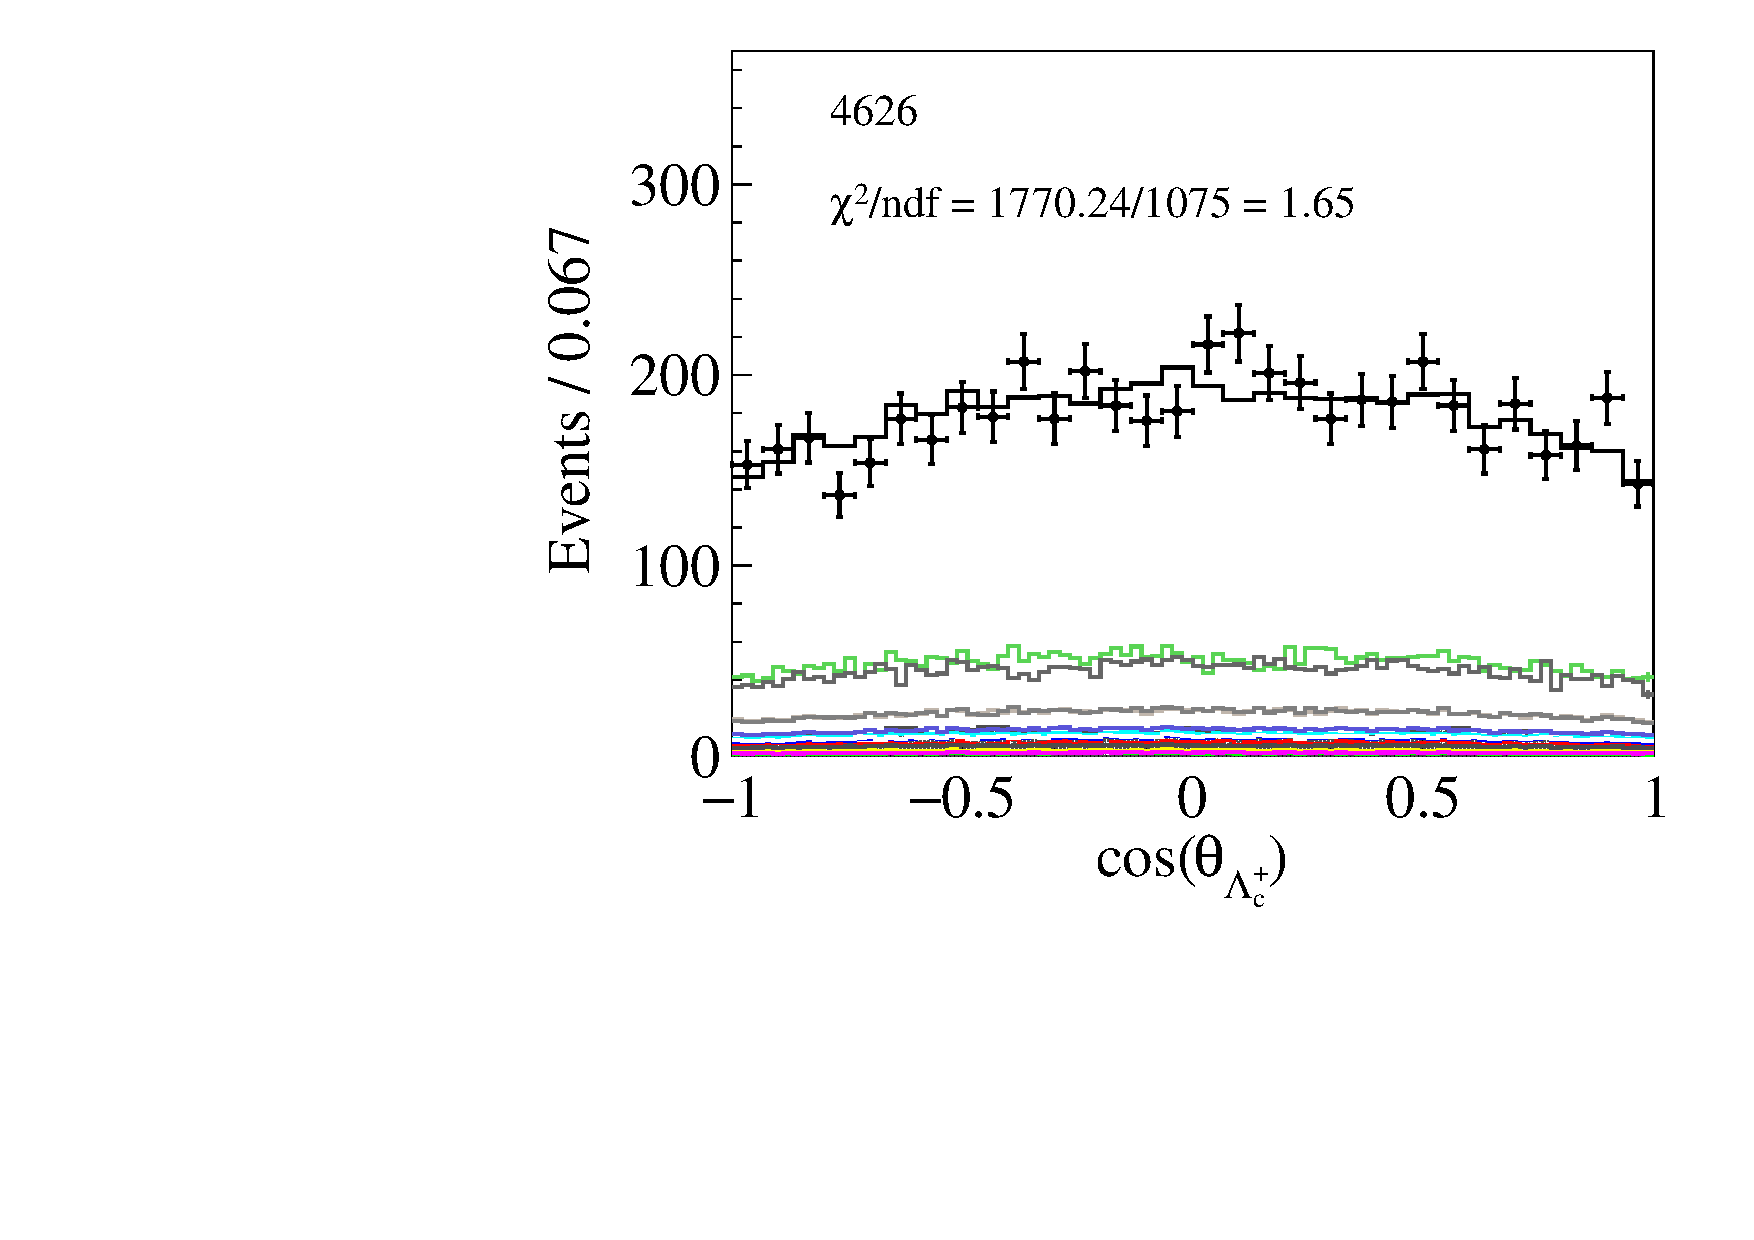
\includegraphics[width=0.24\textwidth]{figure/pwa_nominal/s2_epemDSID_Lmdc_cos_beta.pdf} \\
    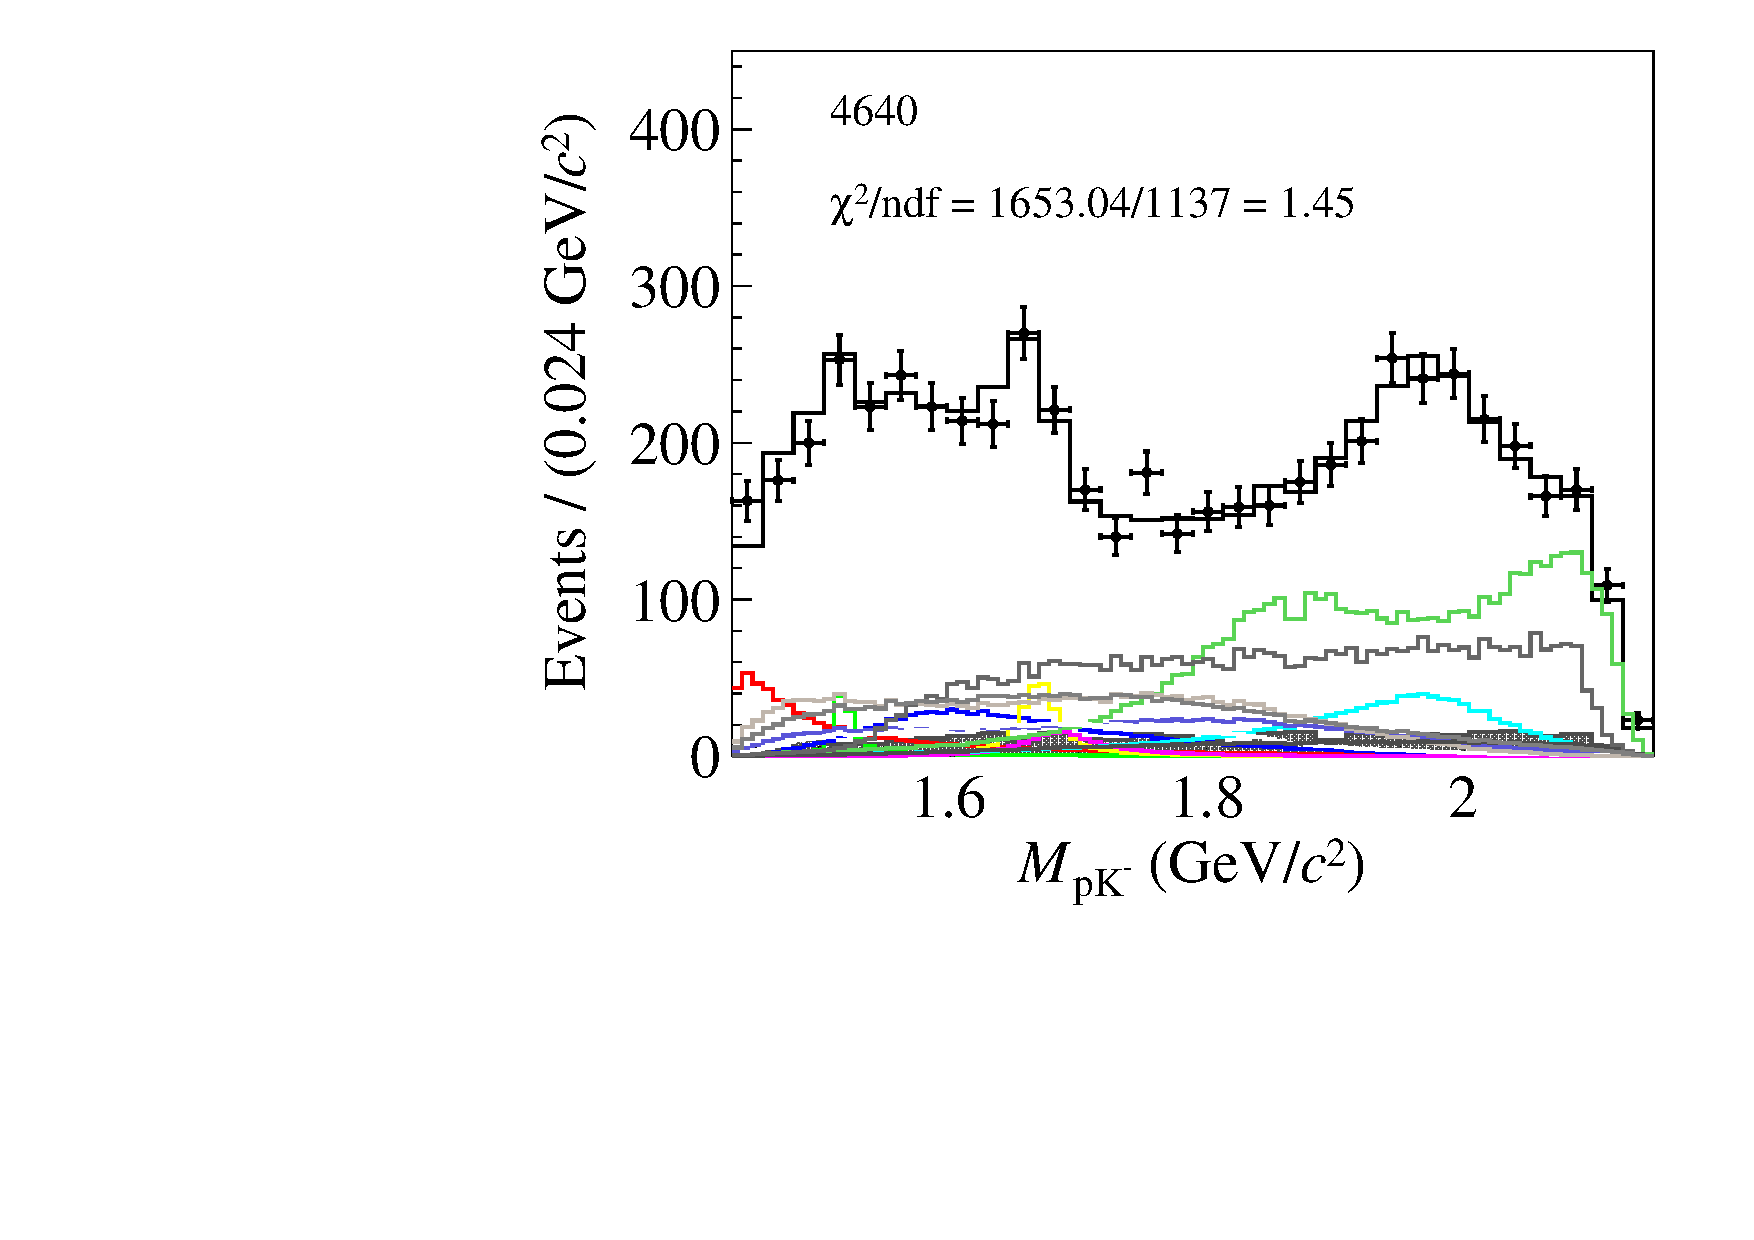
\includegraphics[width=0.24\textwidth]{figure/pwa_nominal/s3_m_R_BC.pdf}
    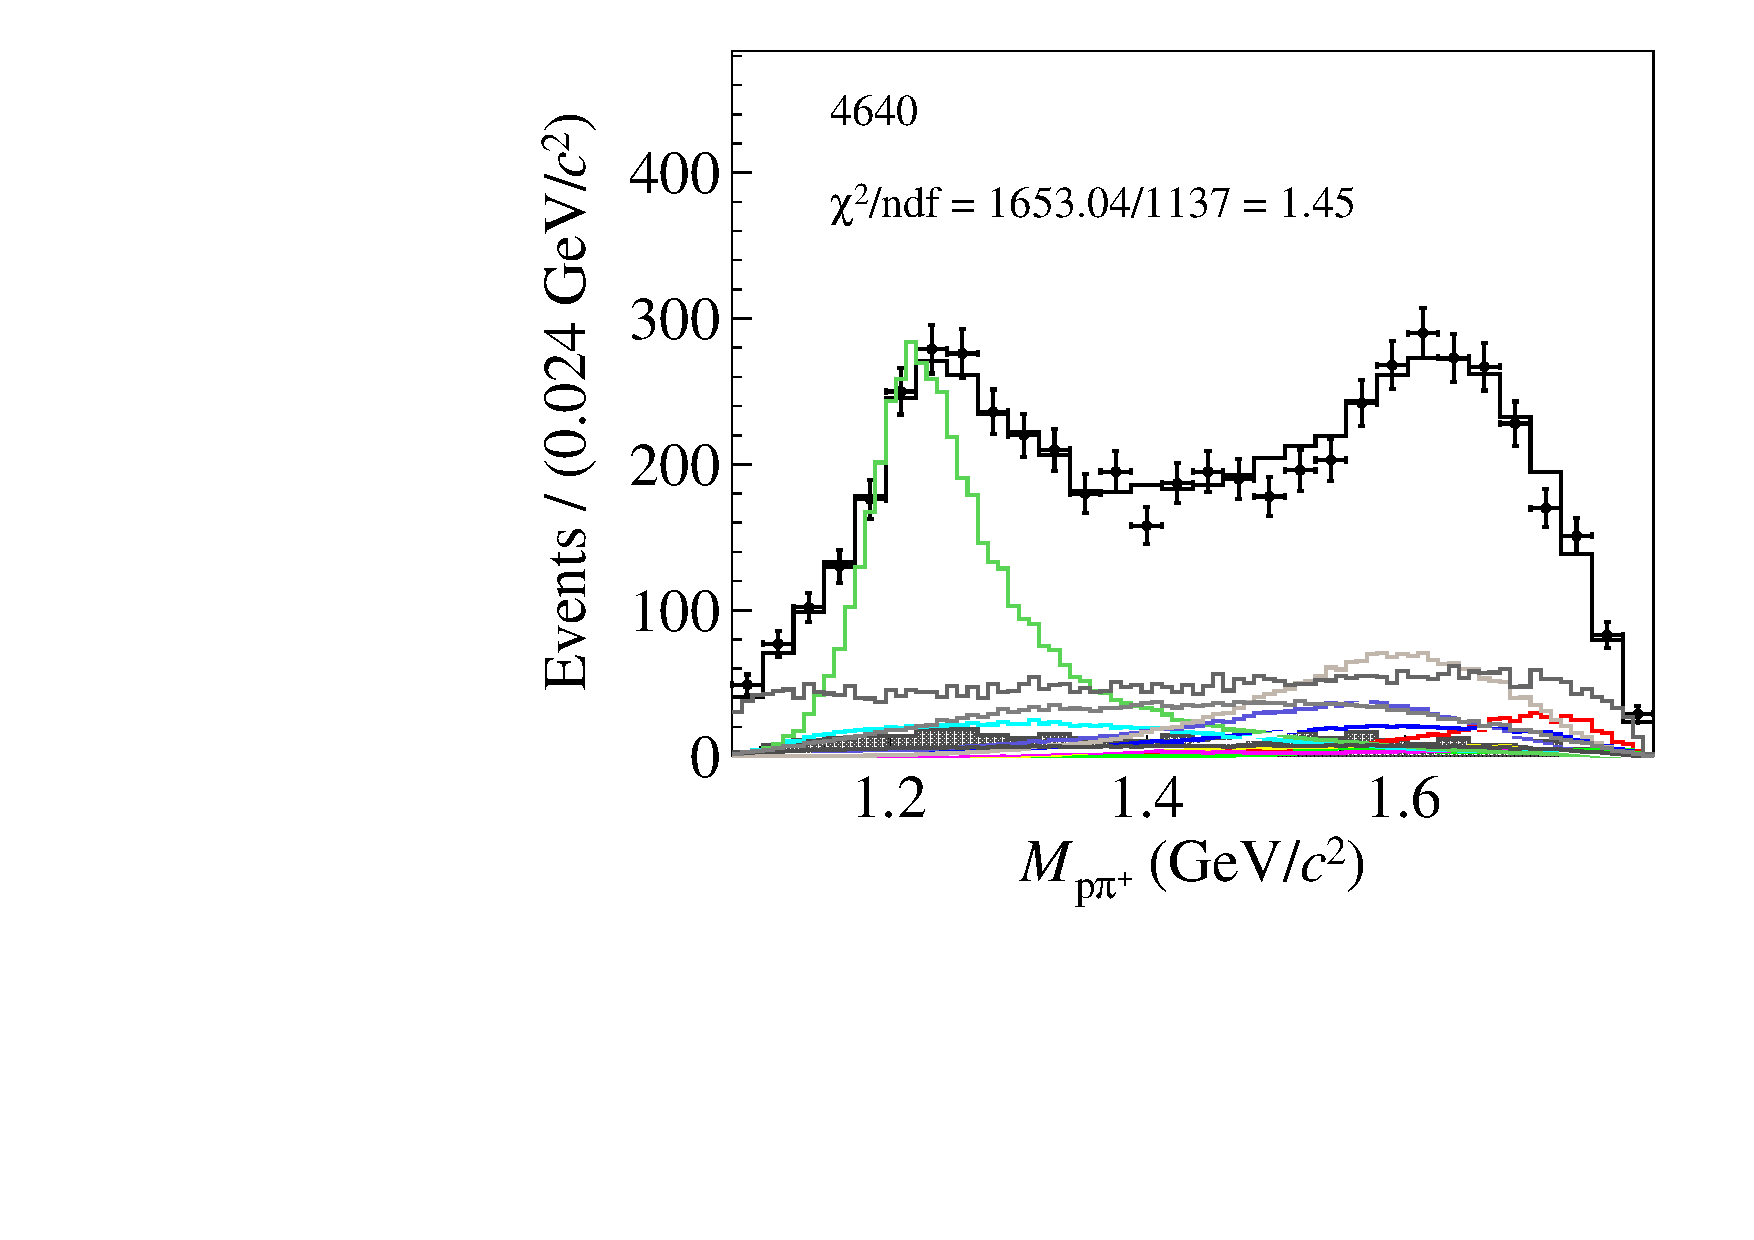
\includegraphics[width=0.24\textwidth]{figure/pwa_nominal/s3_m_R_BD.pdf}
    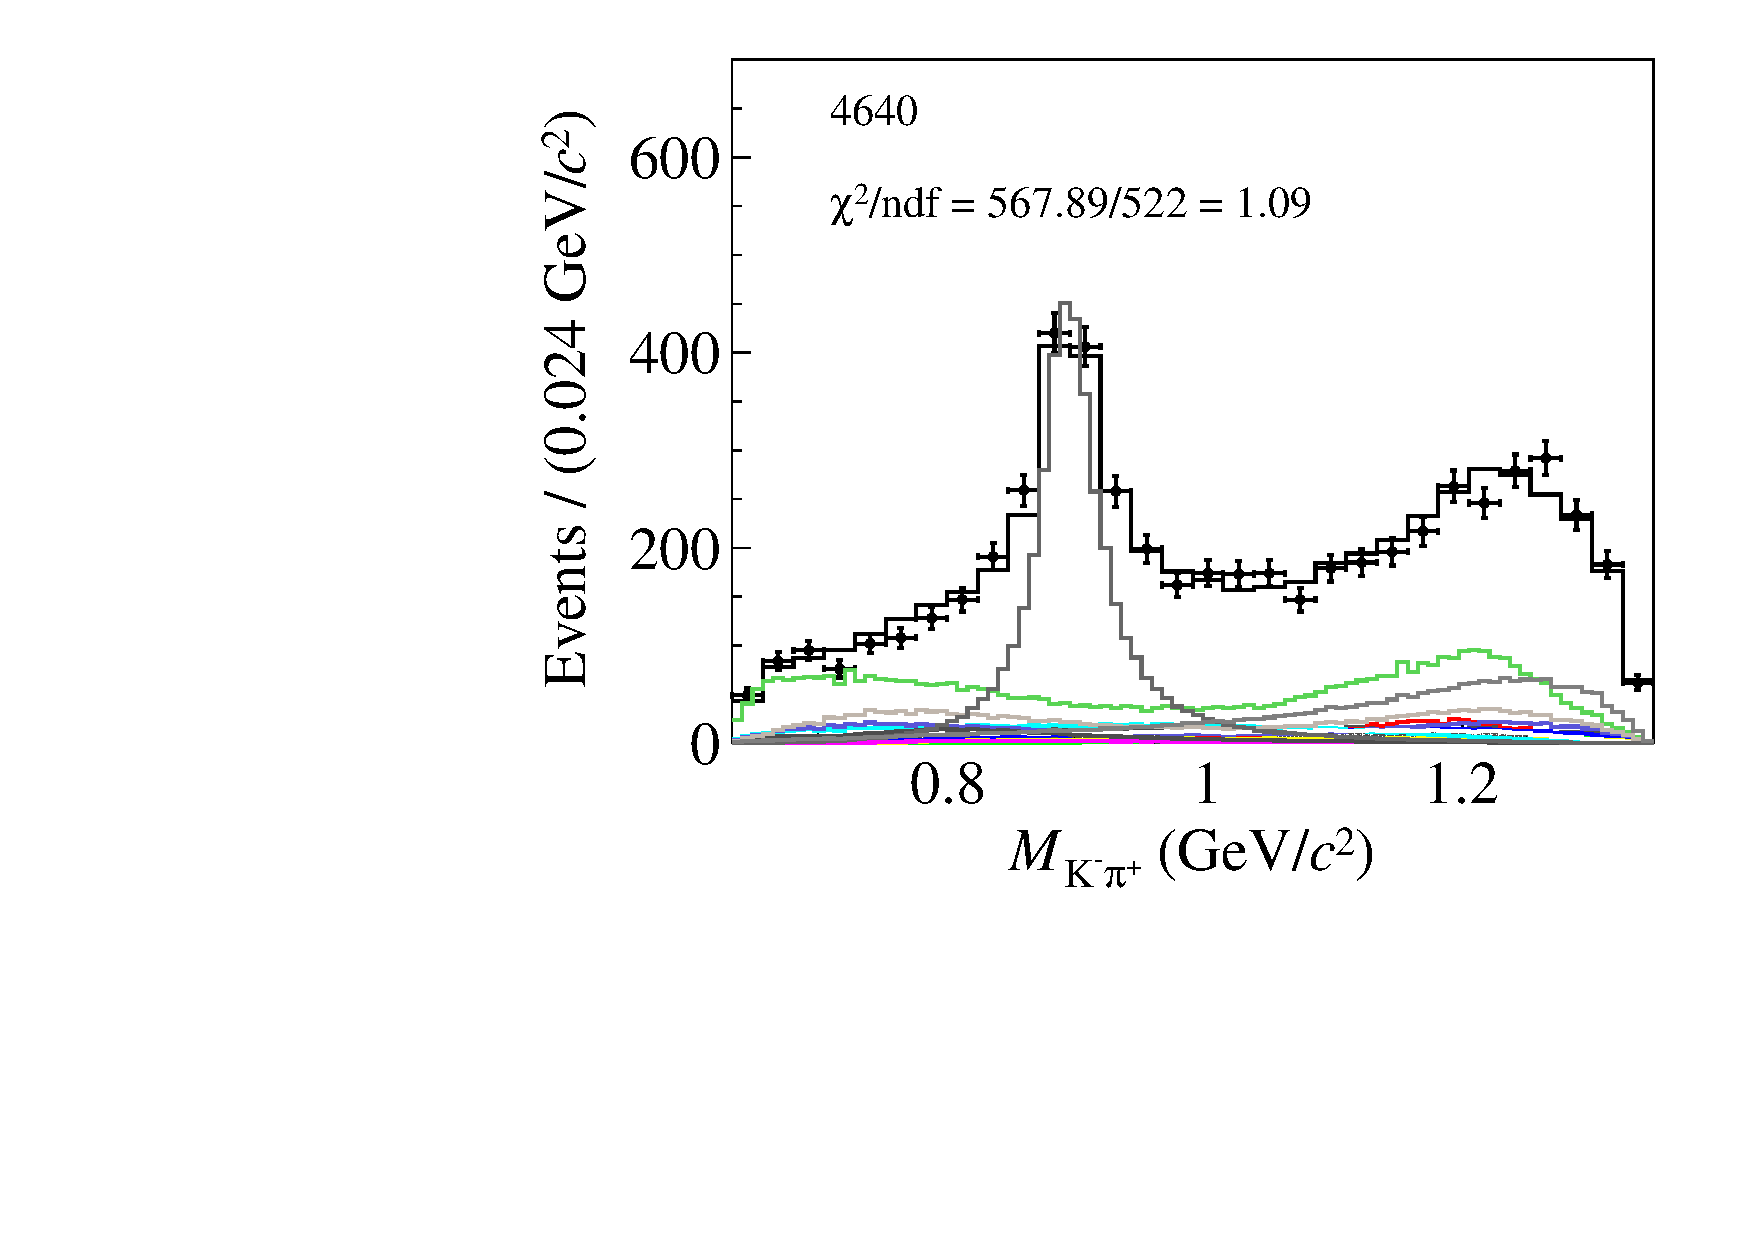
\includegraphics[width=0.24\textwidth]{figure/pwa_nominal/s3_m_R_CD.pdf}
    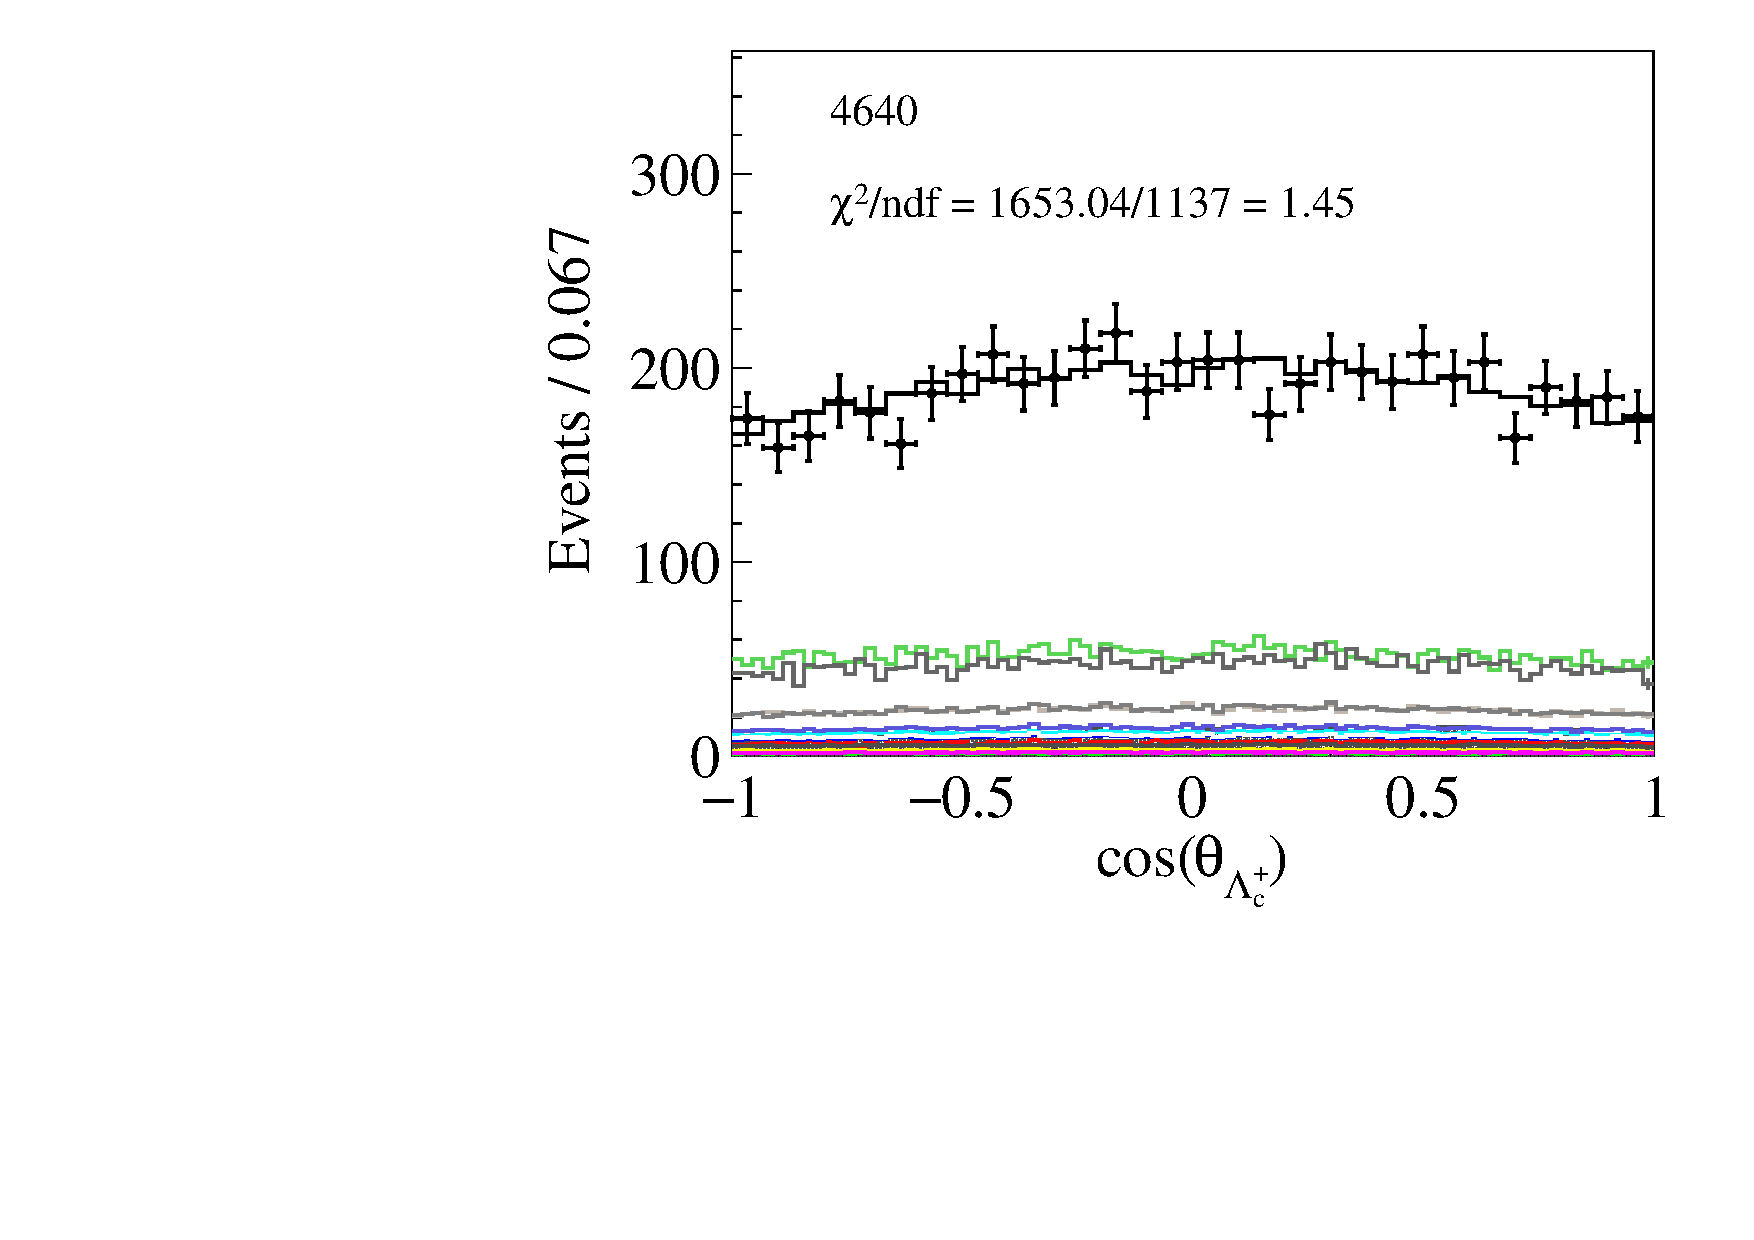
\includegraphics[width=0.24\textwidth]{figure/pwa_nominal/s3_epemDSID_Lmdc_cos_beta.pdf} \\
    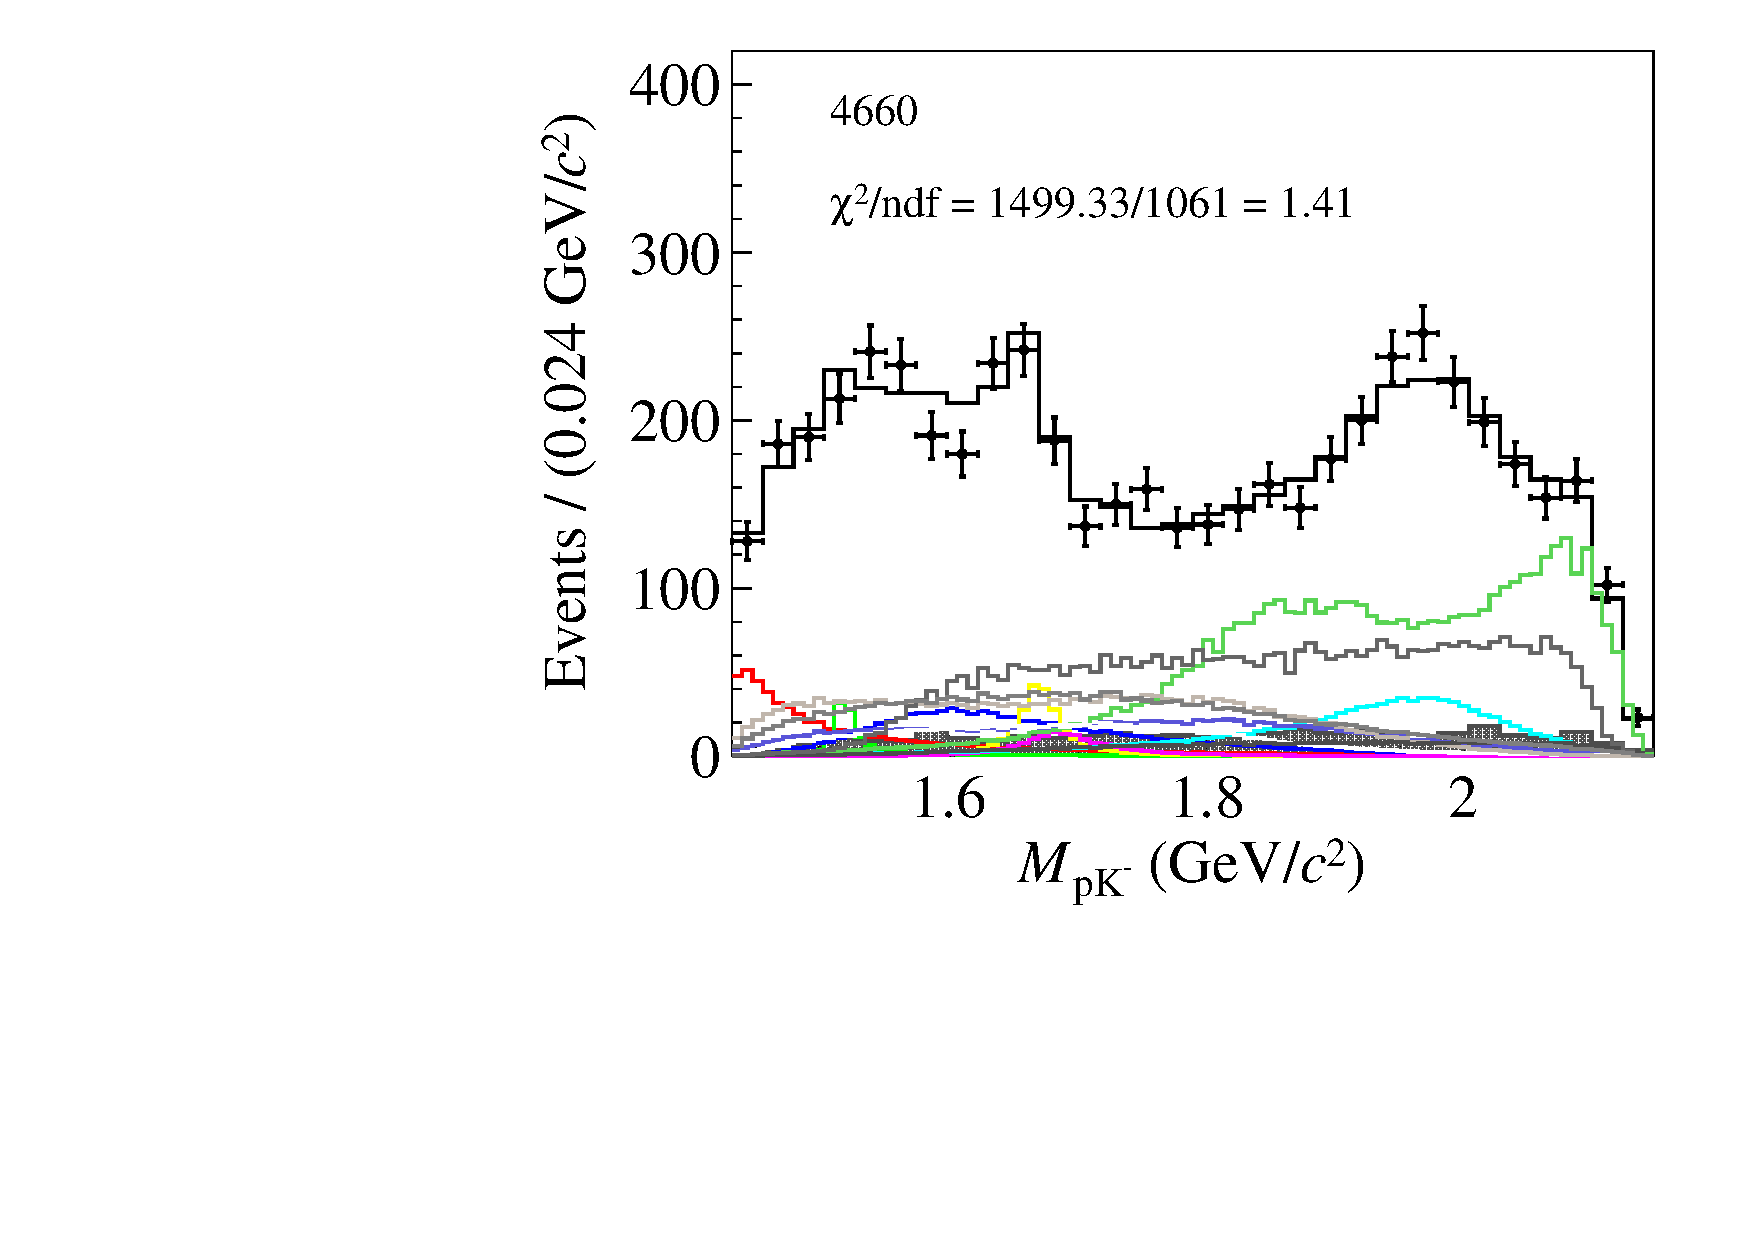
\includegraphics[width=0.24\textwidth]{figure/pwa_nominal/s4_m_R_BC.pdf}
    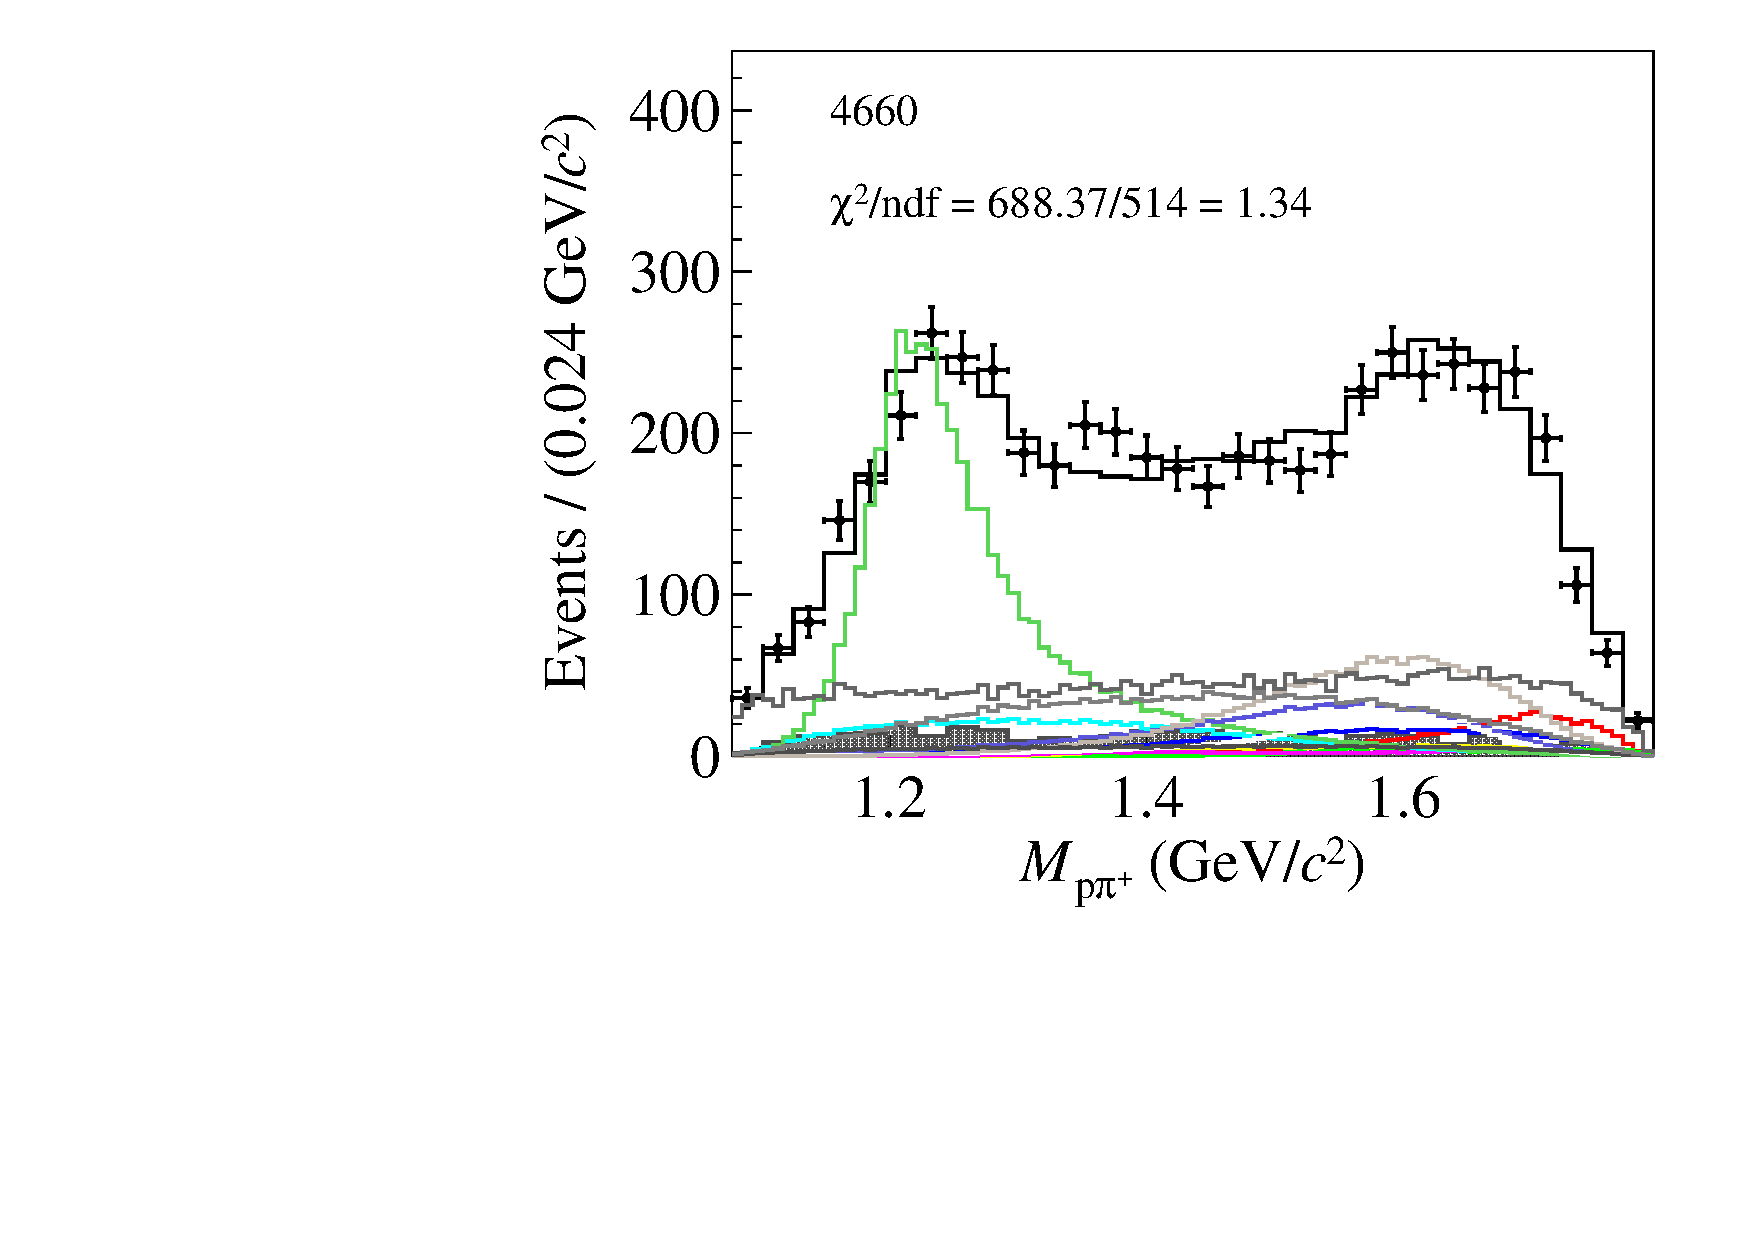
\includegraphics[width=0.24\textwidth]{figure/pwa_nominal/s4_m_R_BD.pdf}
    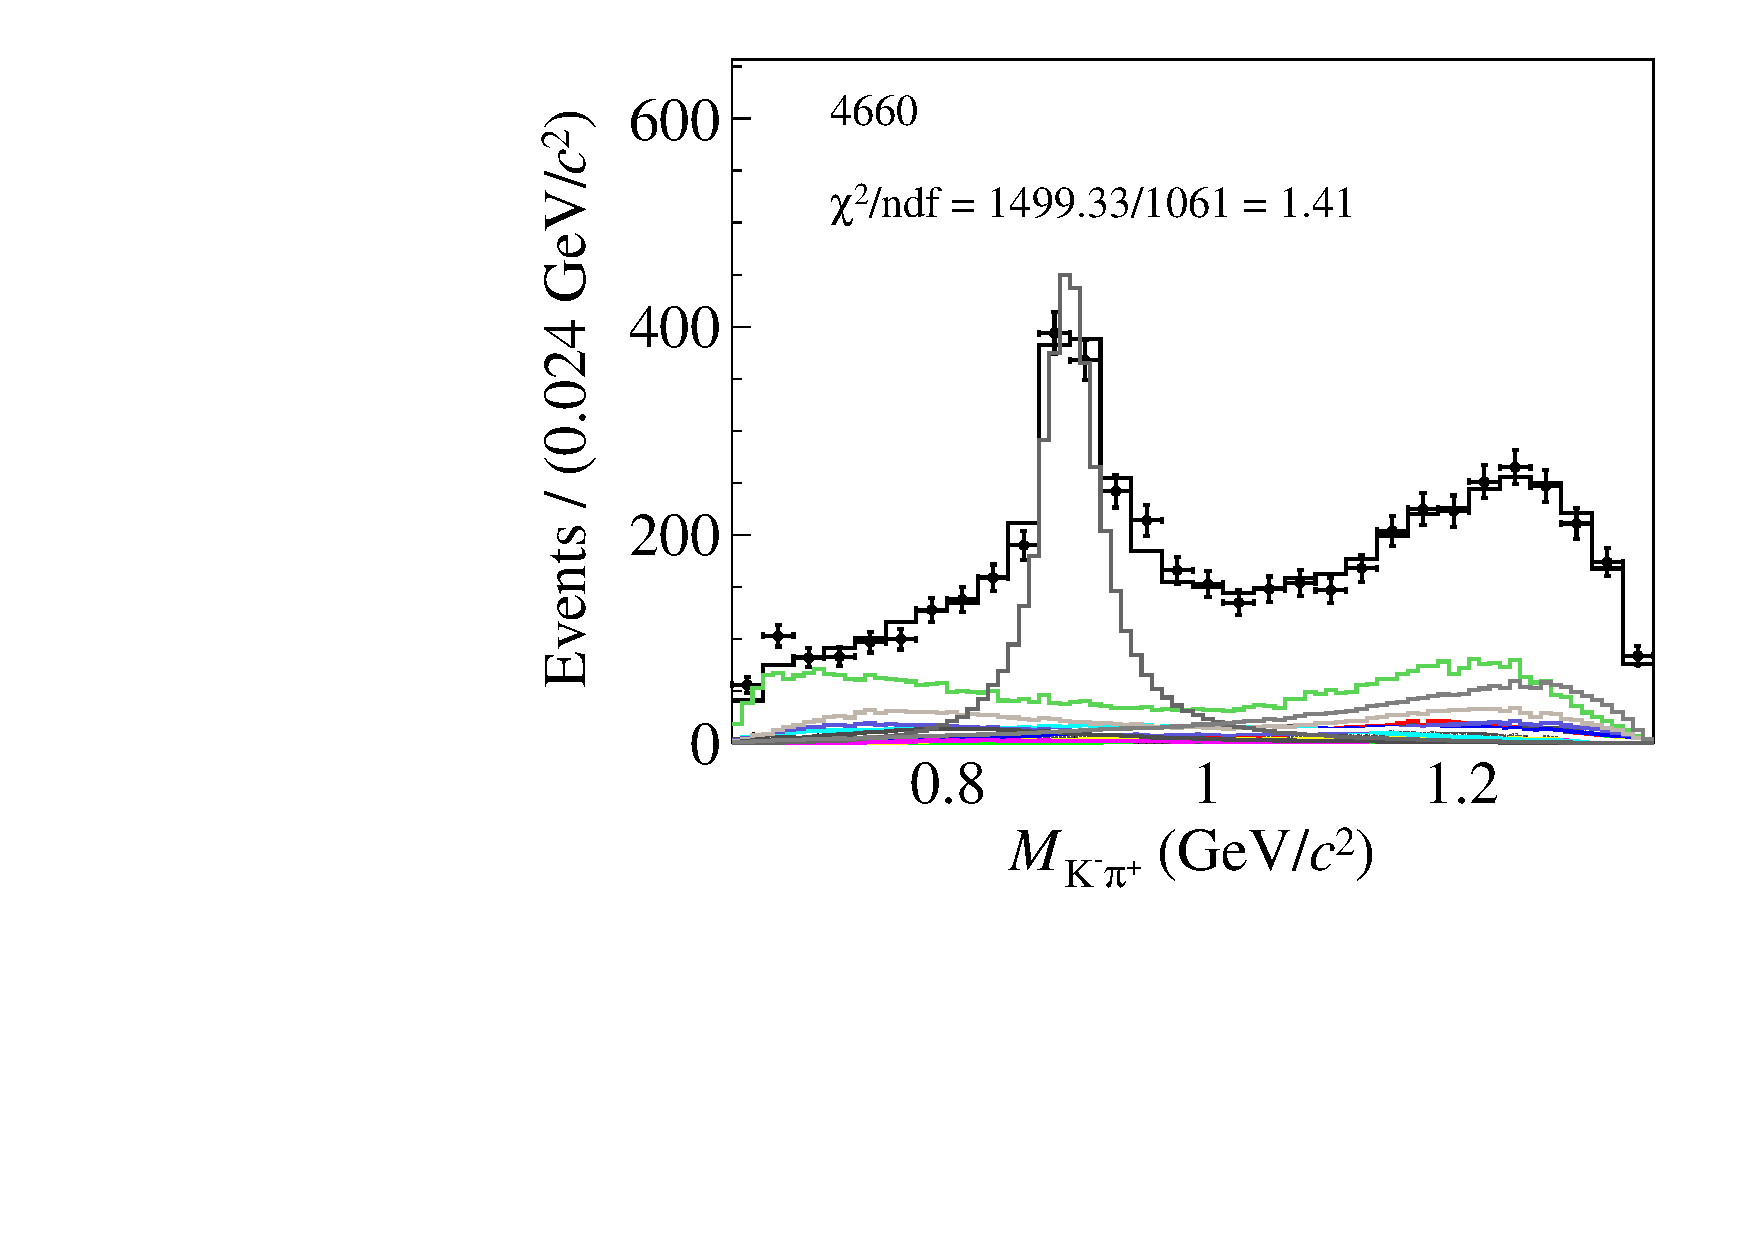
\includegraphics[width=0.24\textwidth]{figure/pwa_nominal/s4_m_R_CD.pdf}
    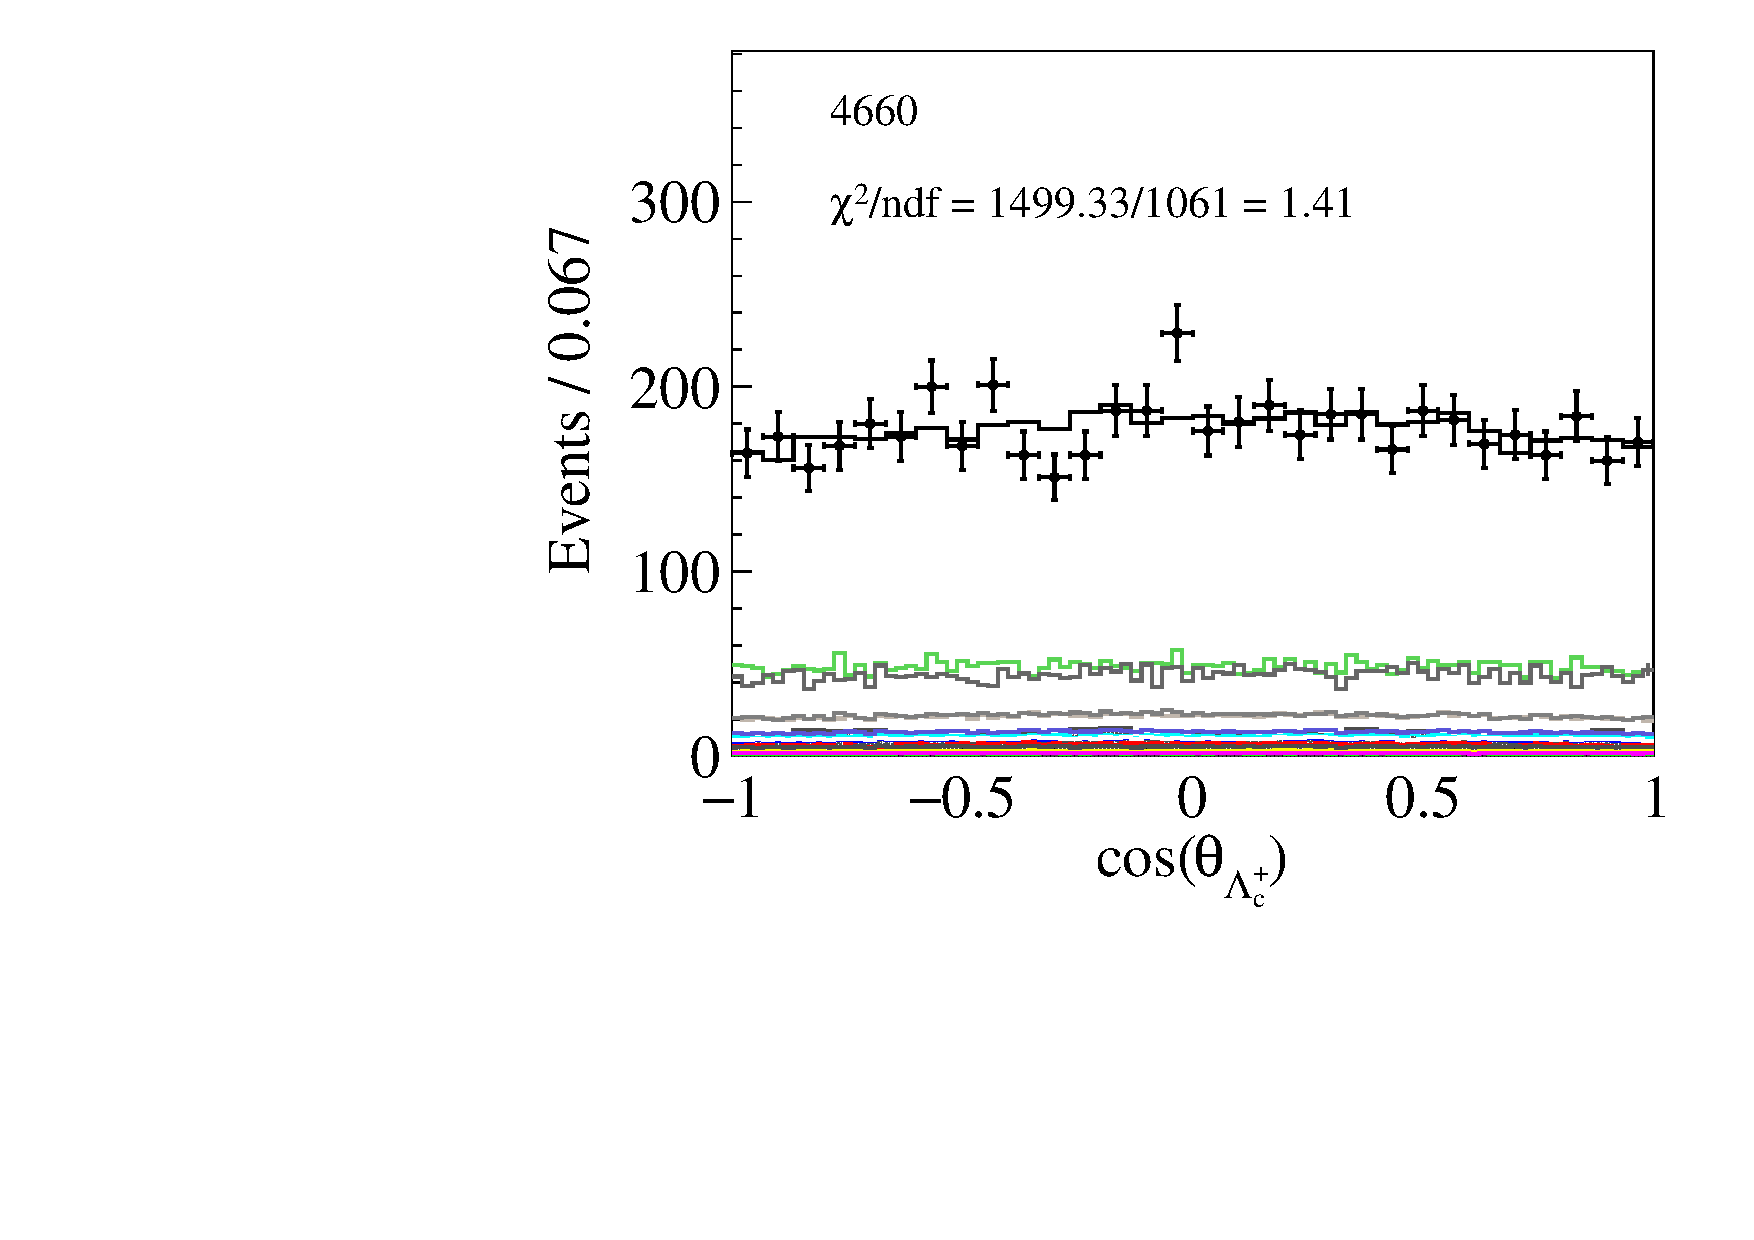
\includegraphics[width=0.24\textwidth]{figure/pwa_nominal/s4_epemDSID_Lmdc_cos_beta.pdf} \\
    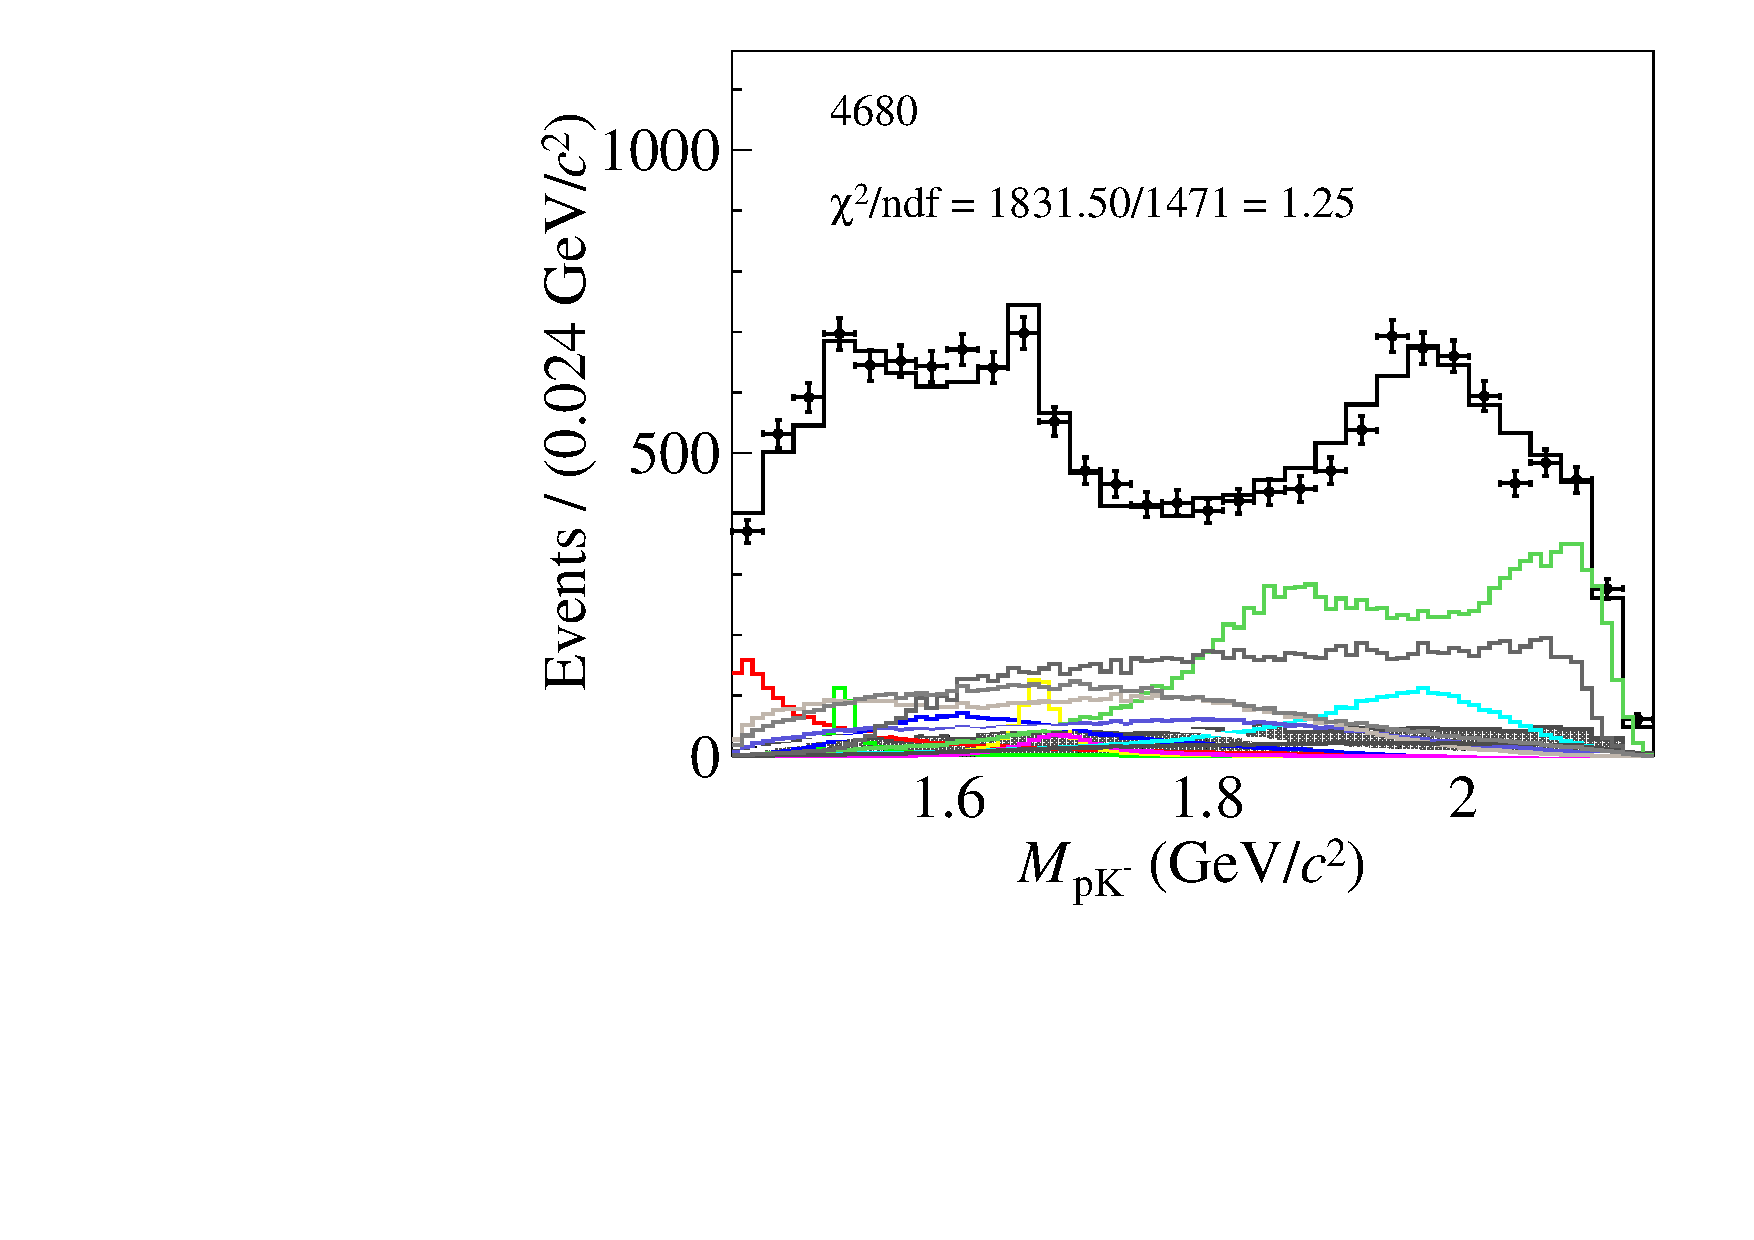
\includegraphics[width=0.24\textwidth]{figure/pwa_nominal/s5_m_R_BC.pdf}
    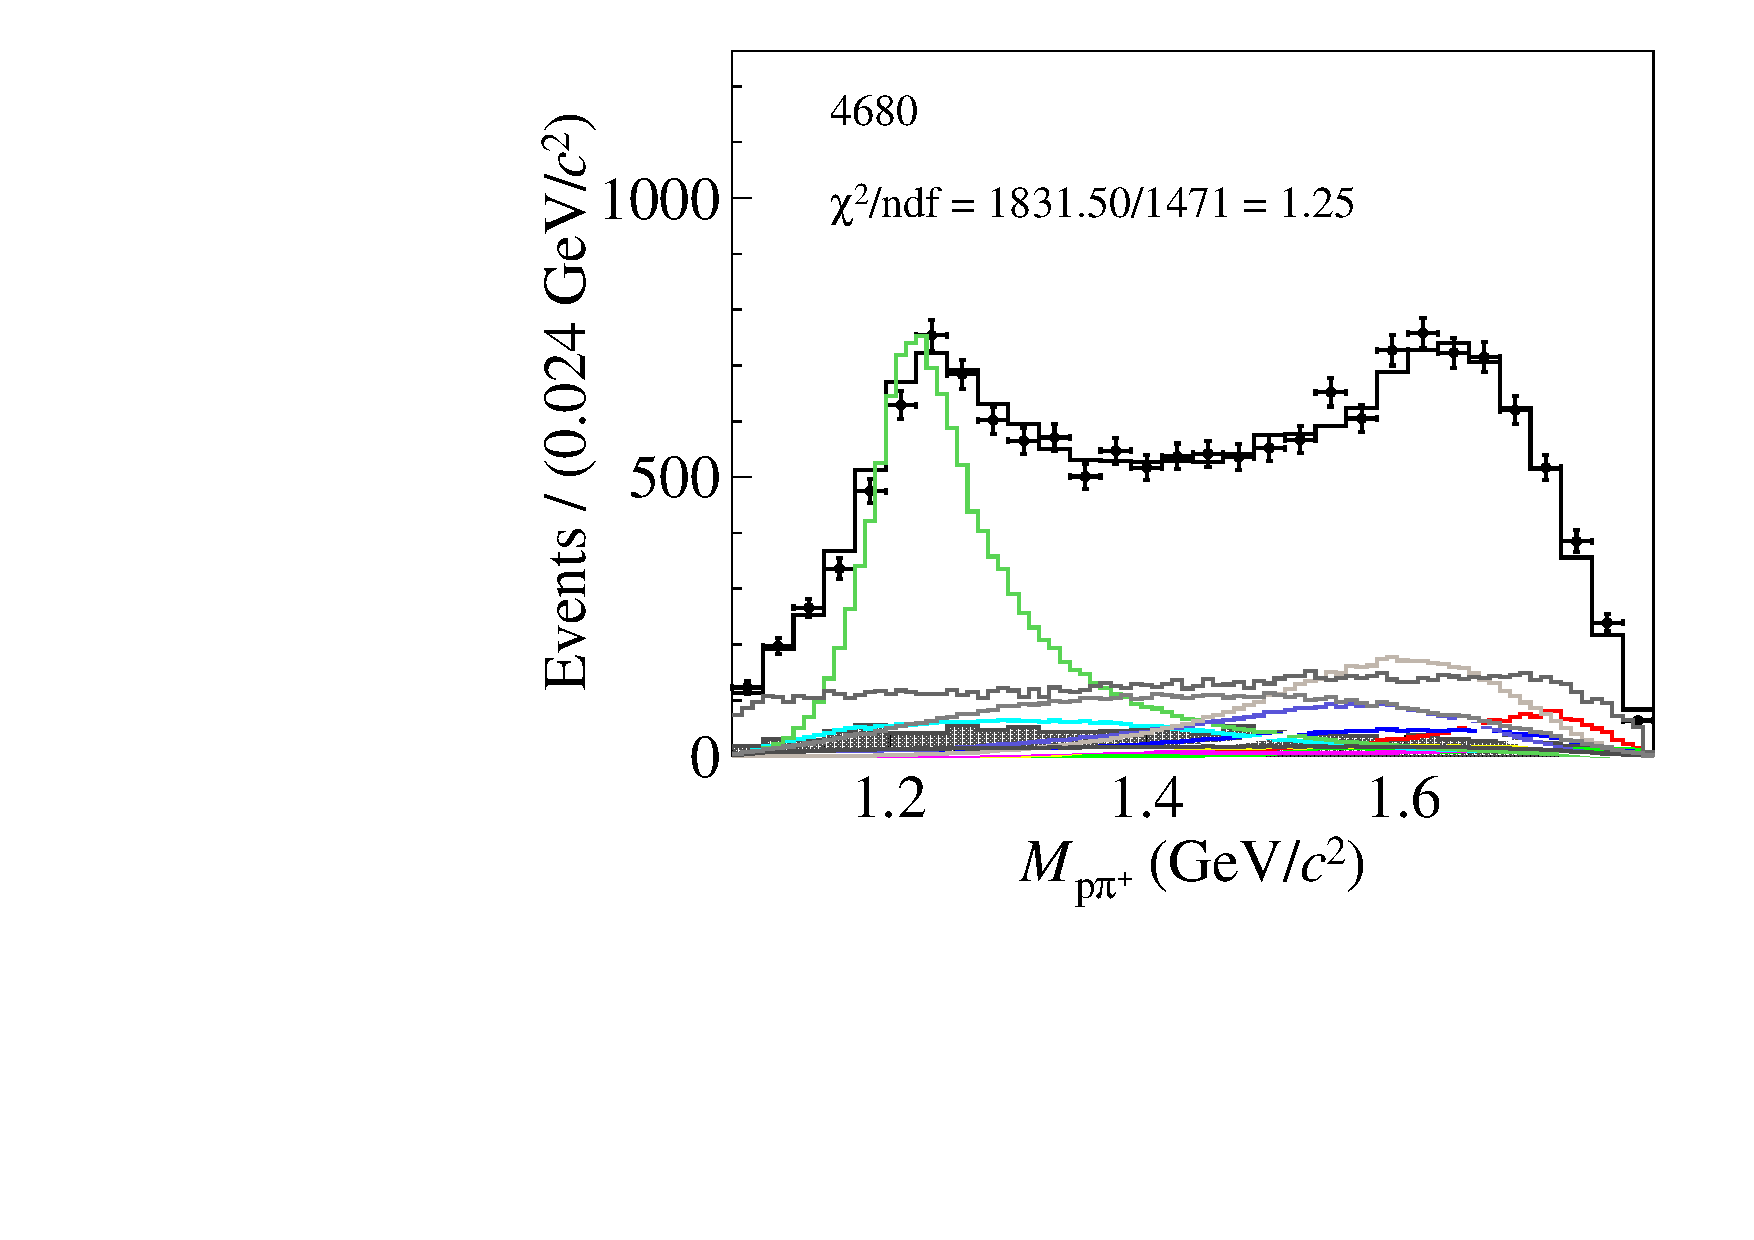
\includegraphics[width=0.24\textwidth]{figure/pwa_nominal/s5_m_R_BD.pdf}
    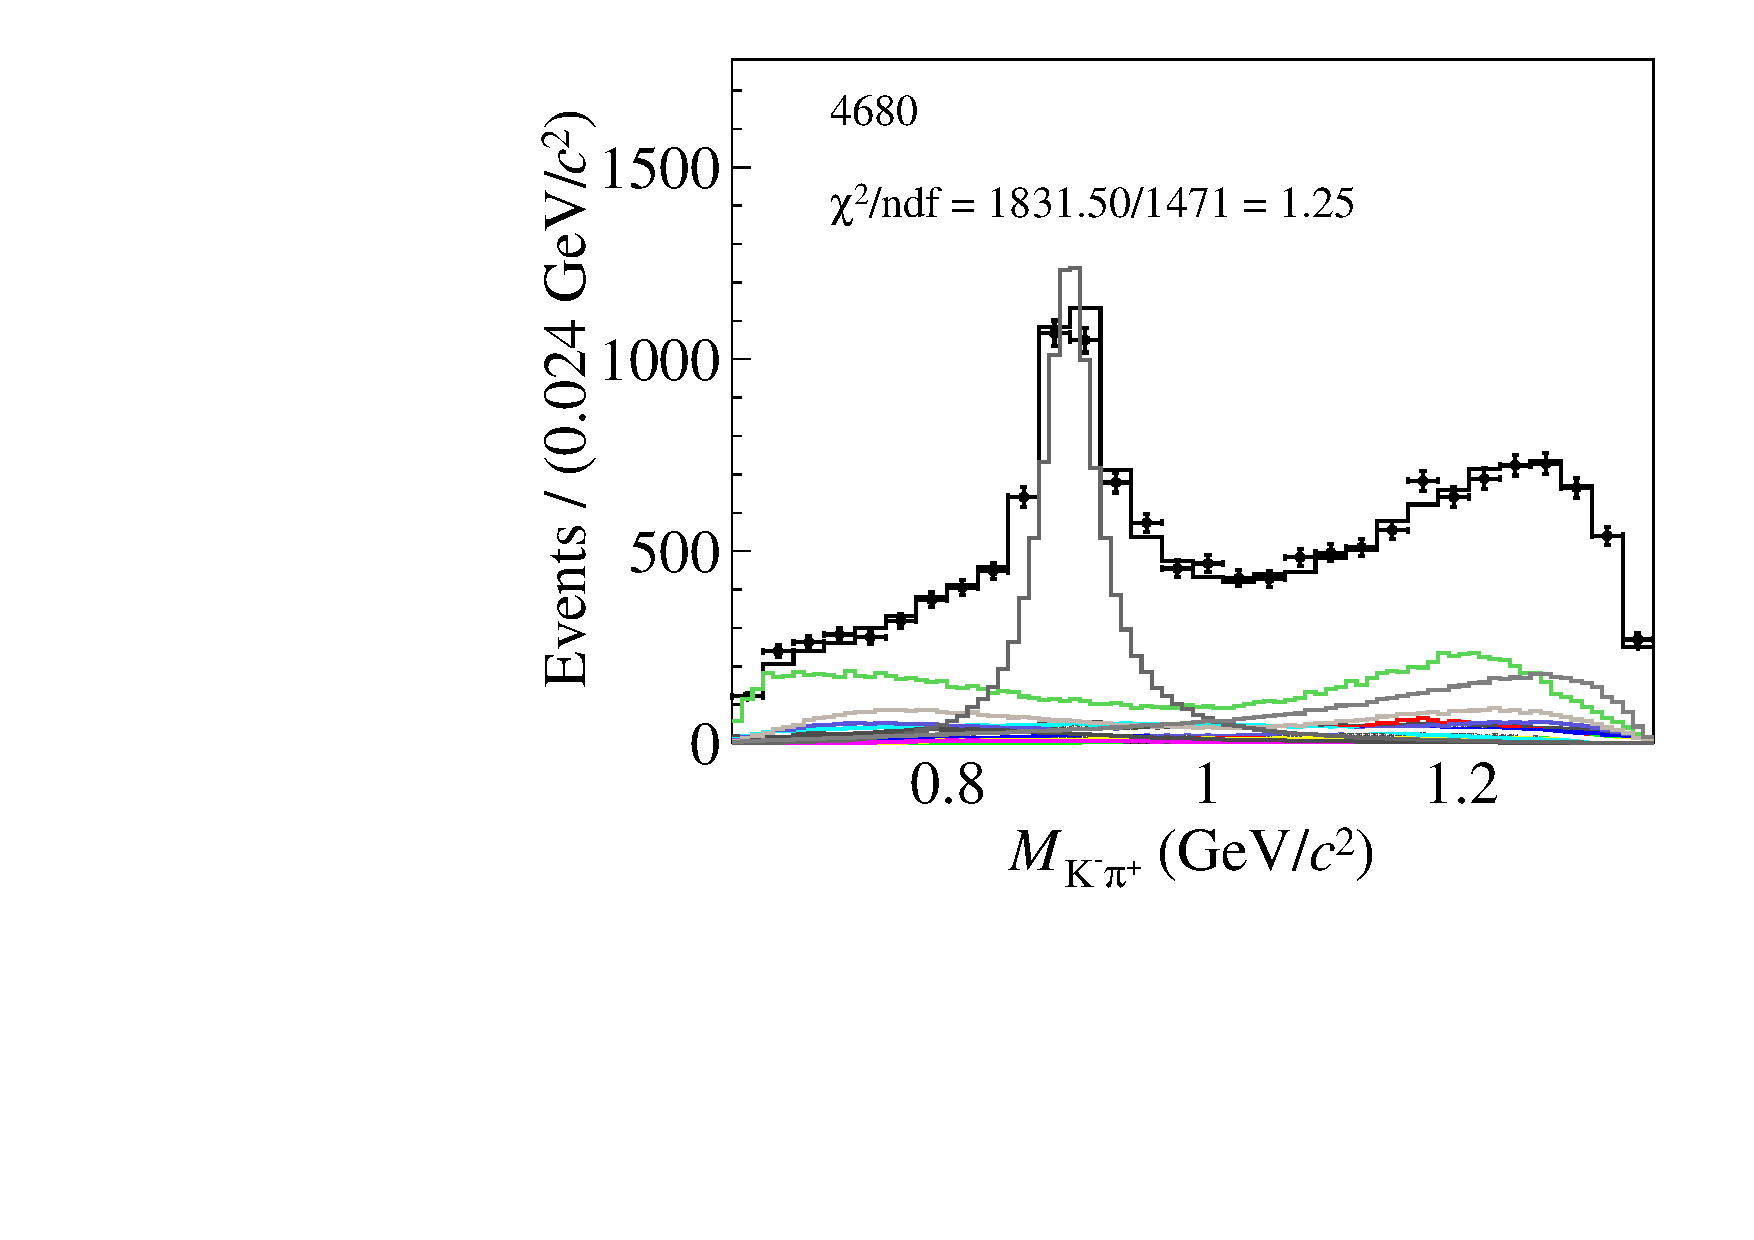
\includegraphics[width=0.24\textwidth]{figure/pwa_nominal/s5_m_R_CD.pdf}
    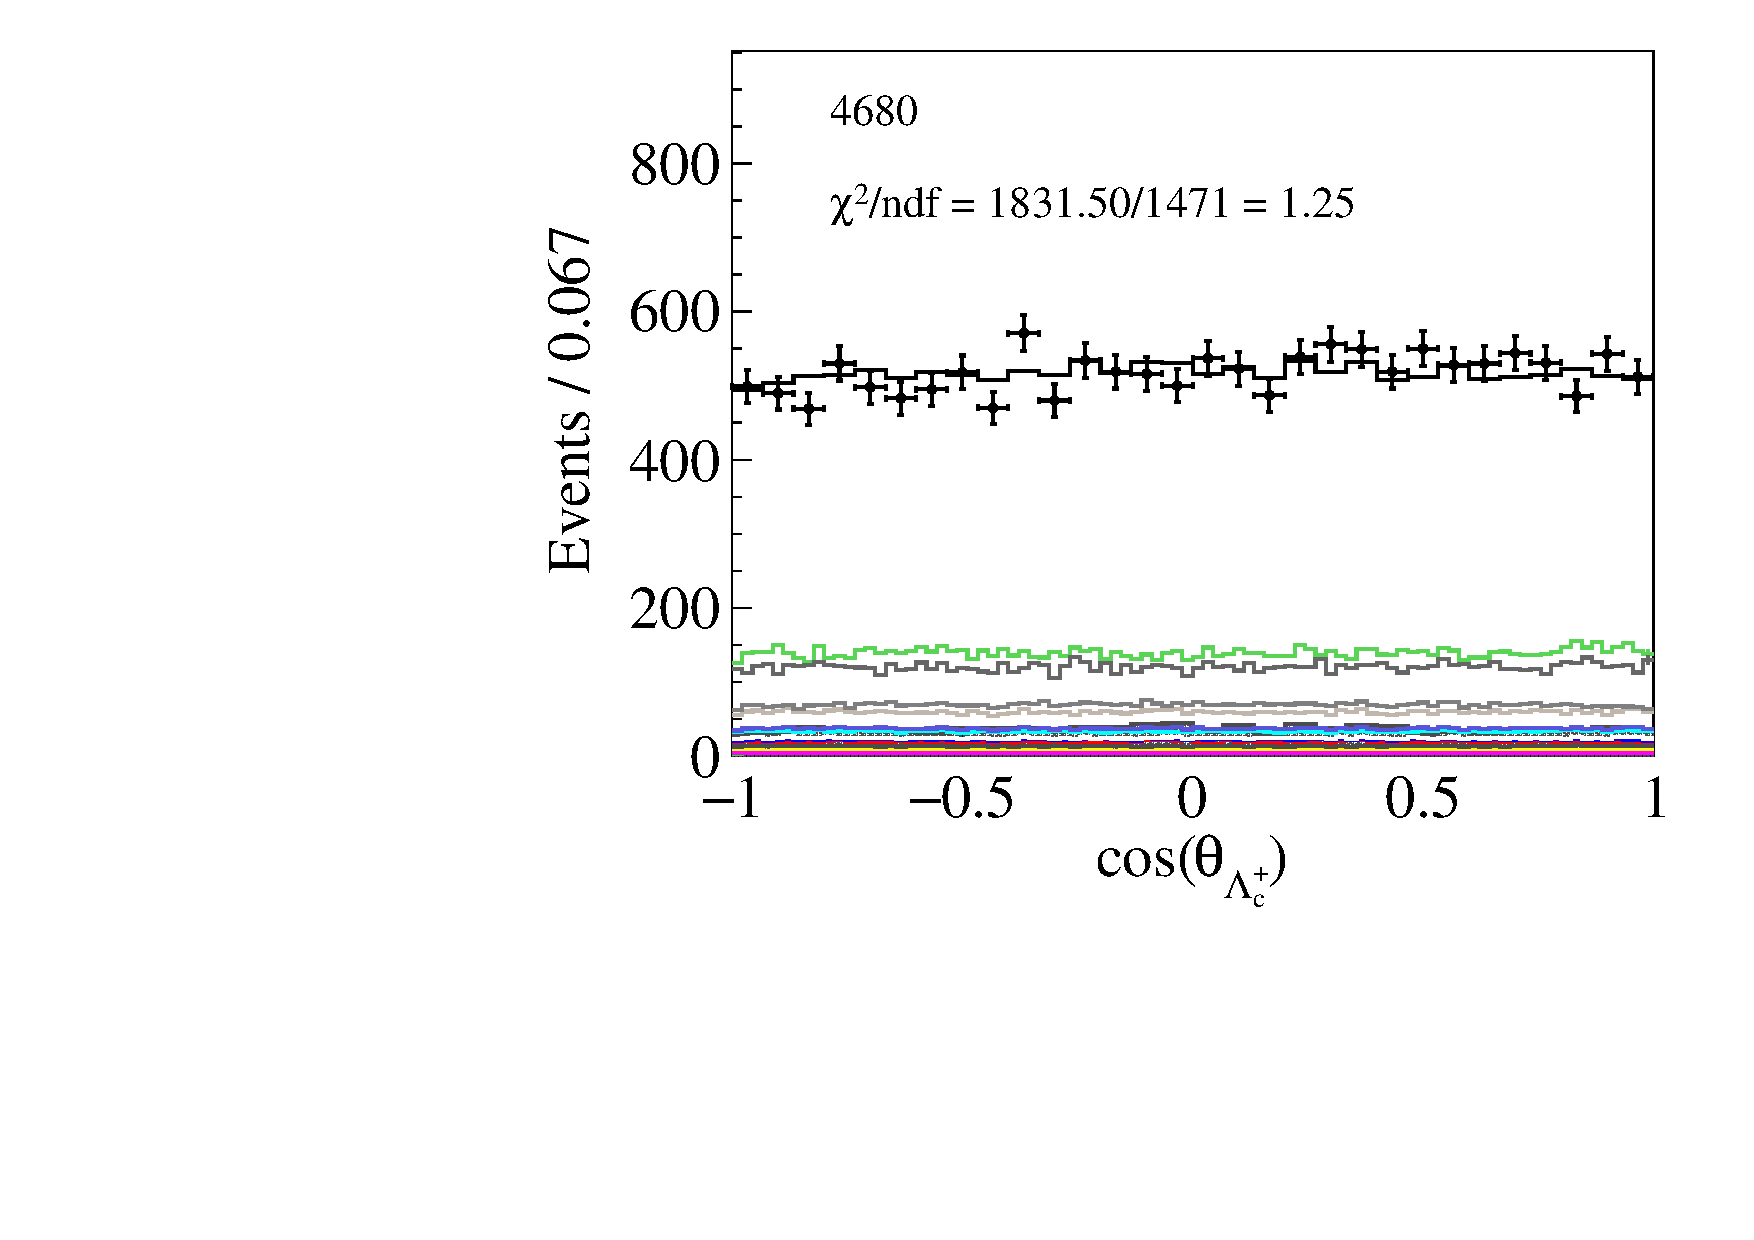
\includegraphics[width=0.24\textwidth]{figure/pwa_nominal/s5_epemDSID_Lmdc_cos_beta.pdf} \\
    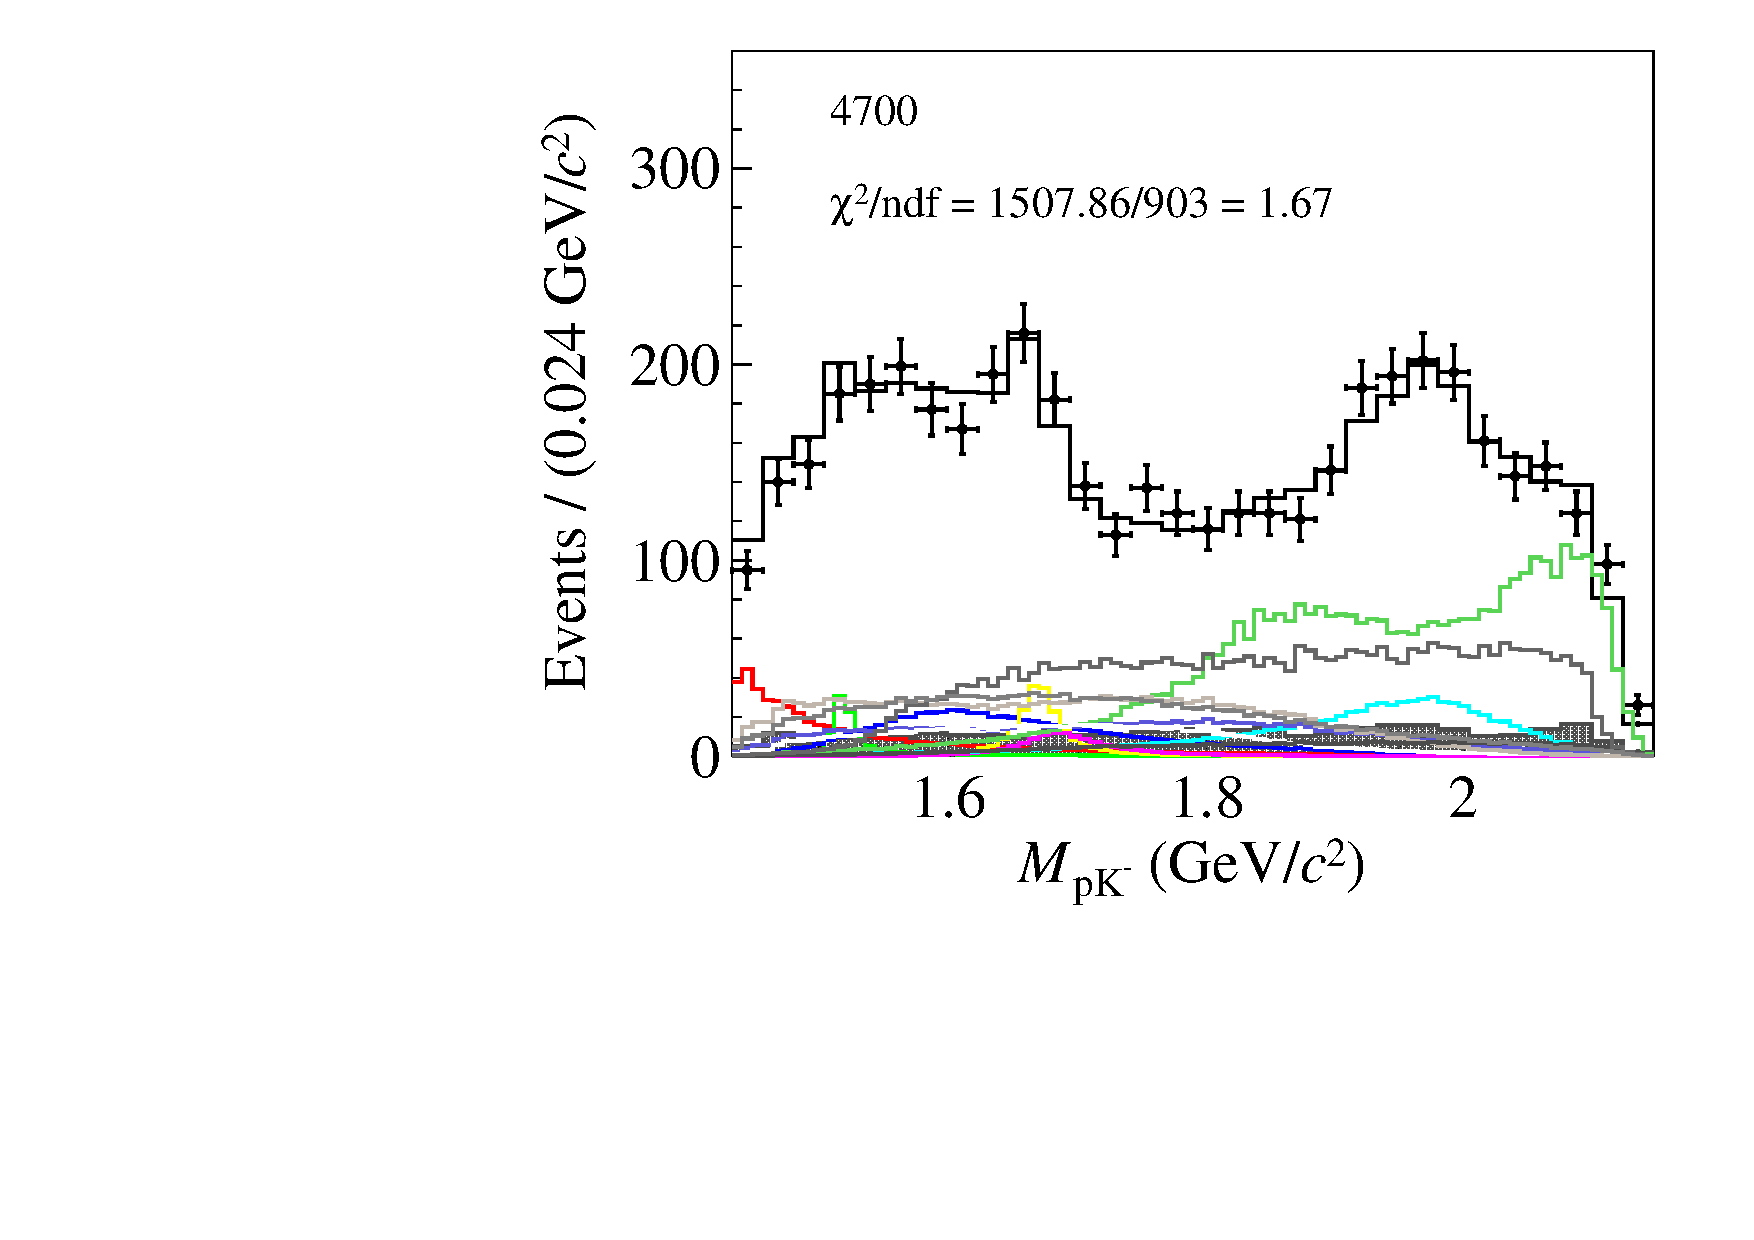
\includegraphics[width=0.24\textwidth]{figure/pwa_nominal/s6_m_R_BC.pdf}
    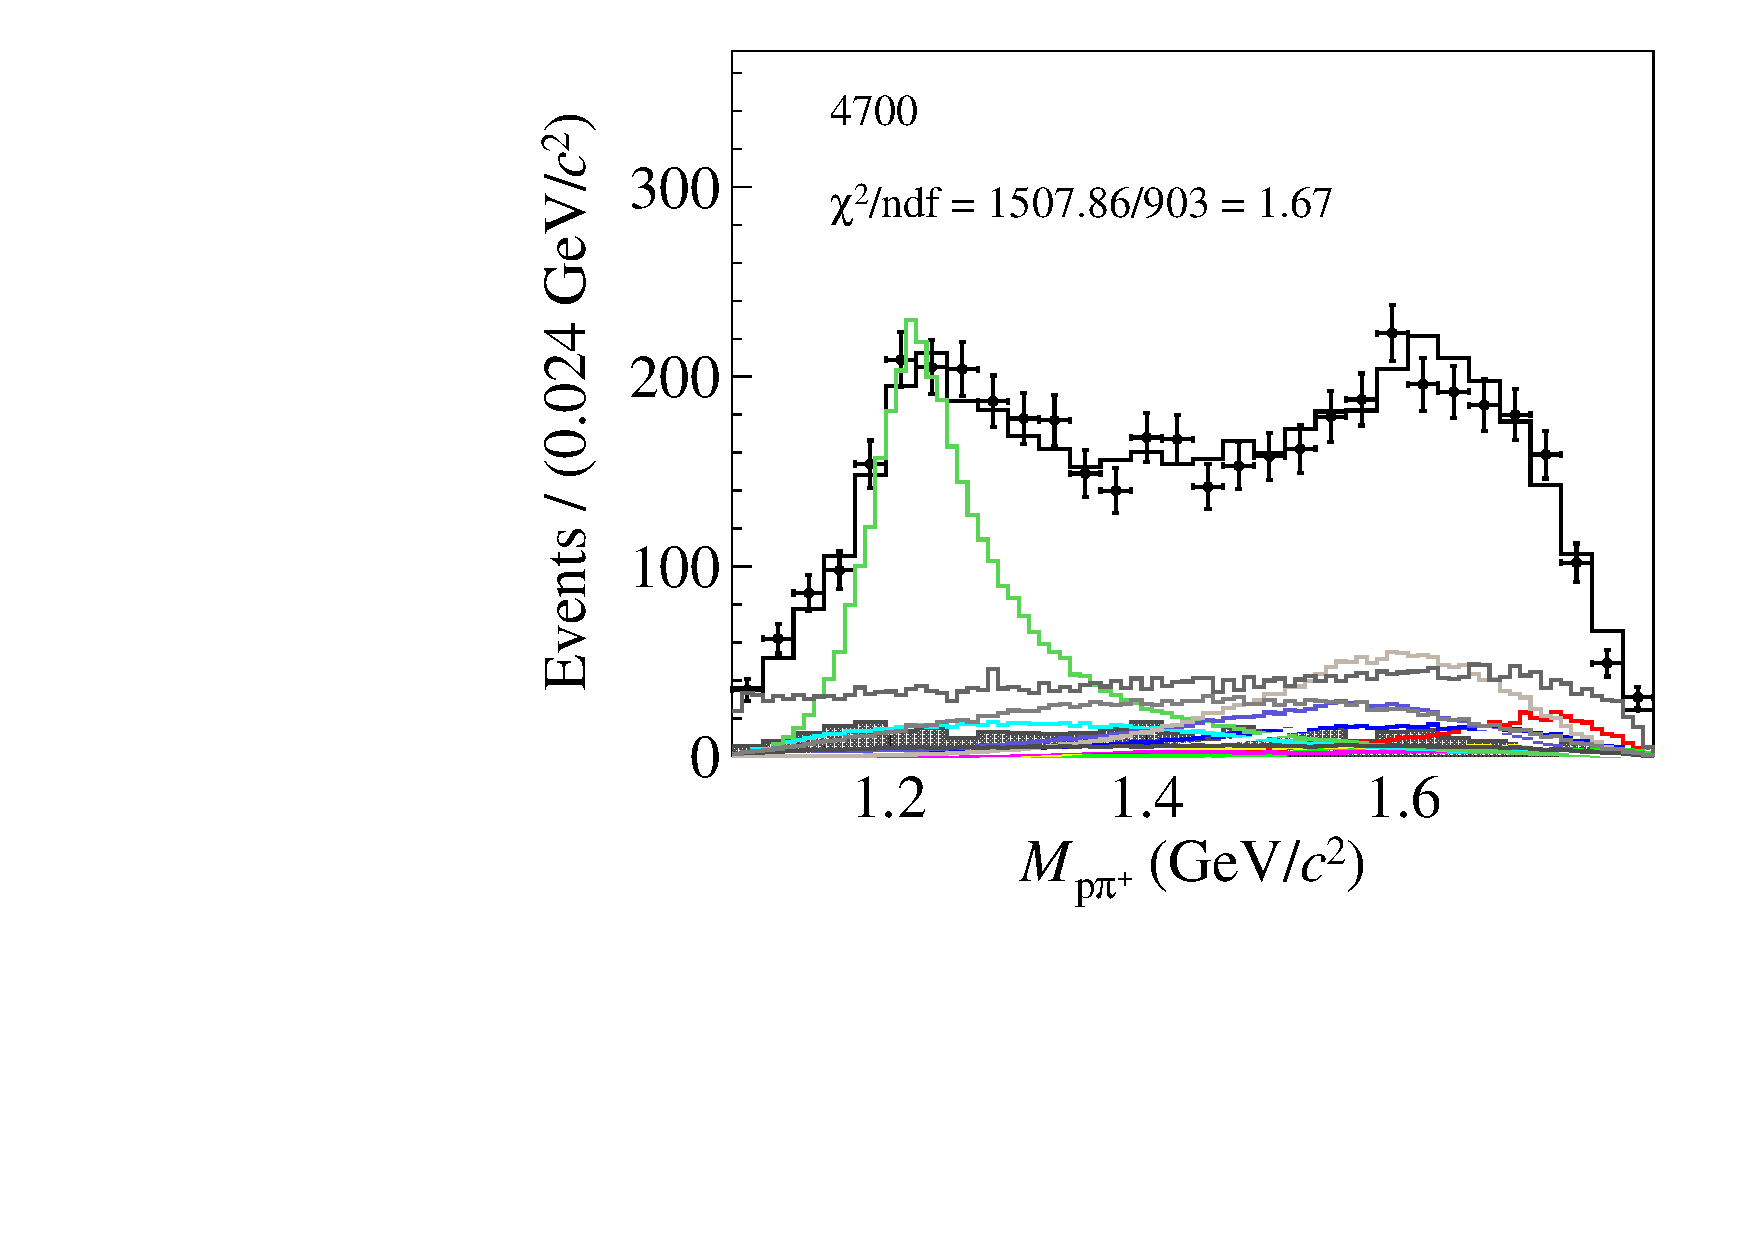
\includegraphics[width=0.24\textwidth]{figure/pwa_nominal/s6_m_R_BD.pdf}
    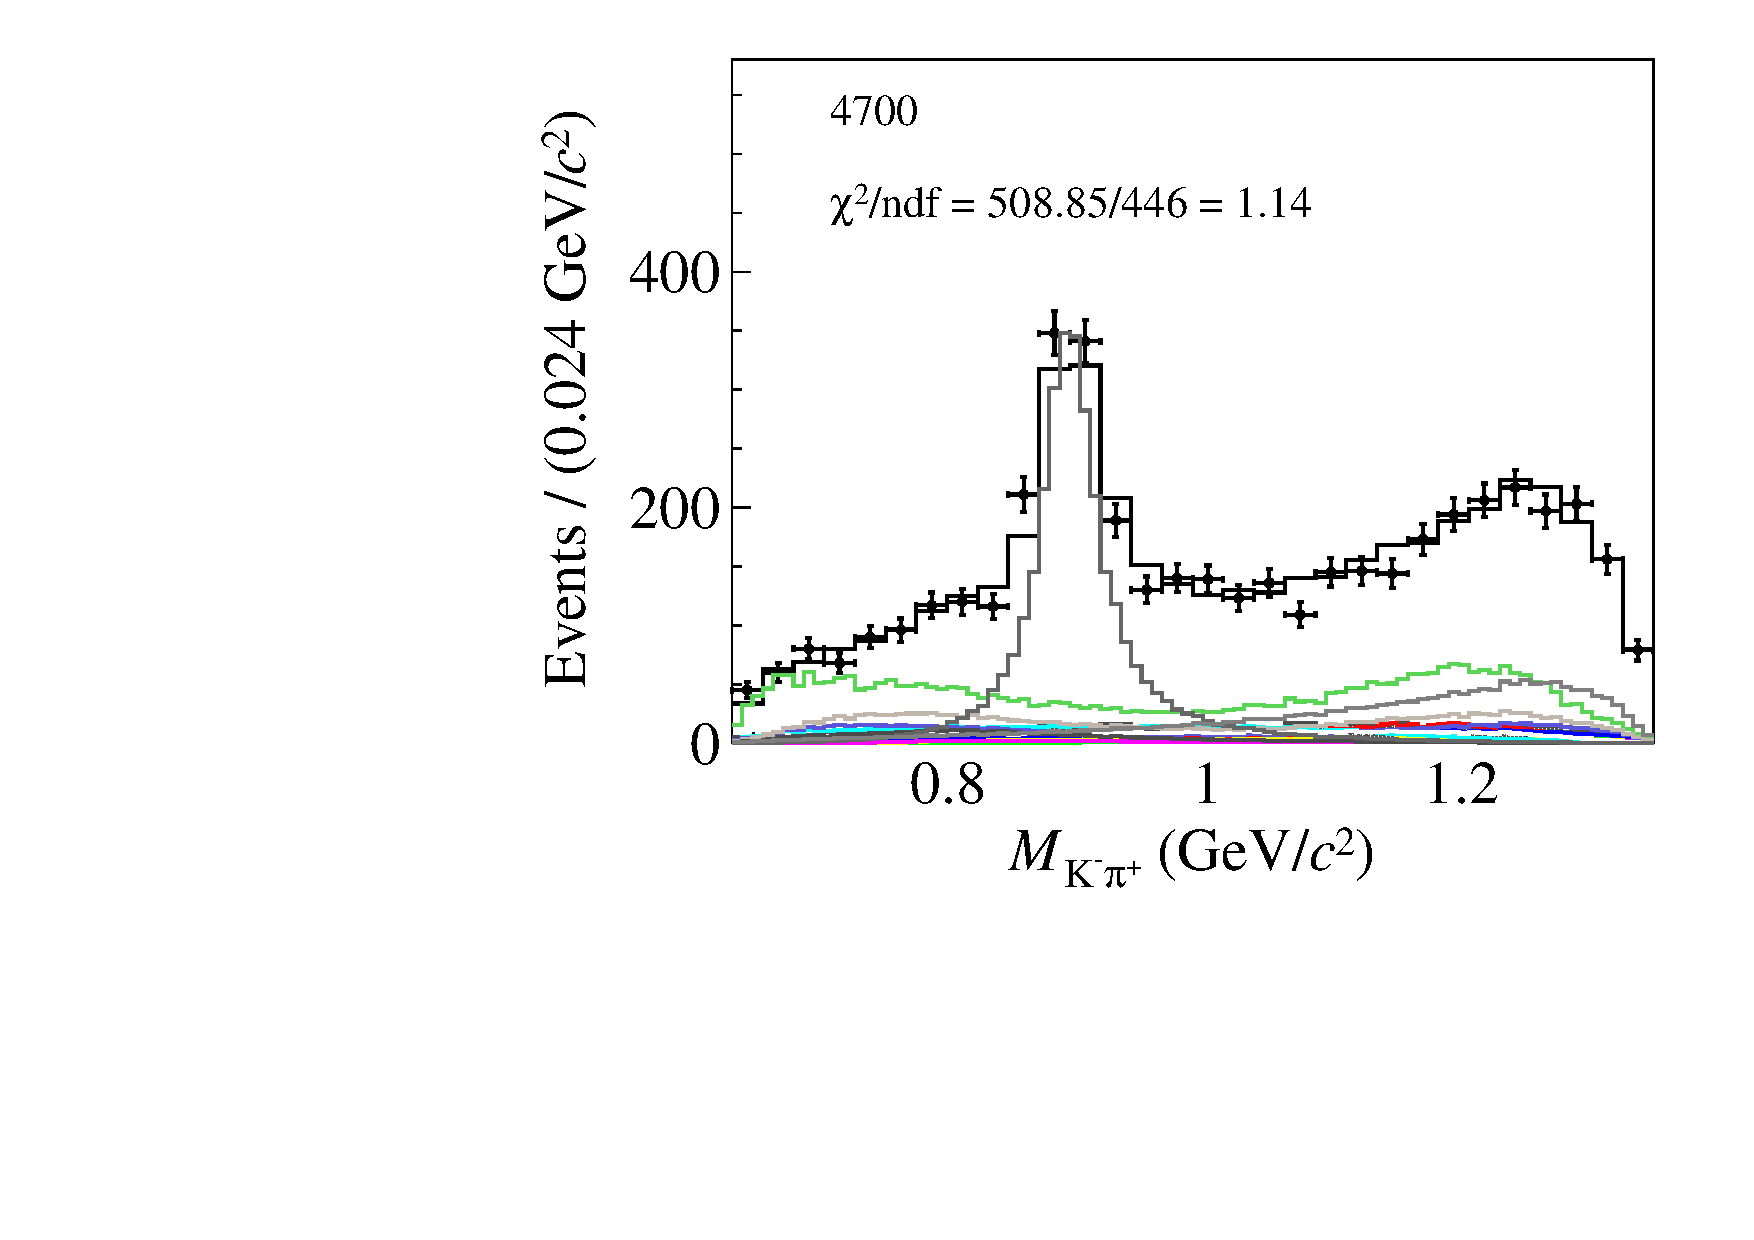
\includegraphics[width=0.24\textwidth]{figure/pwa_nominal/s6_m_R_CD.pdf}
    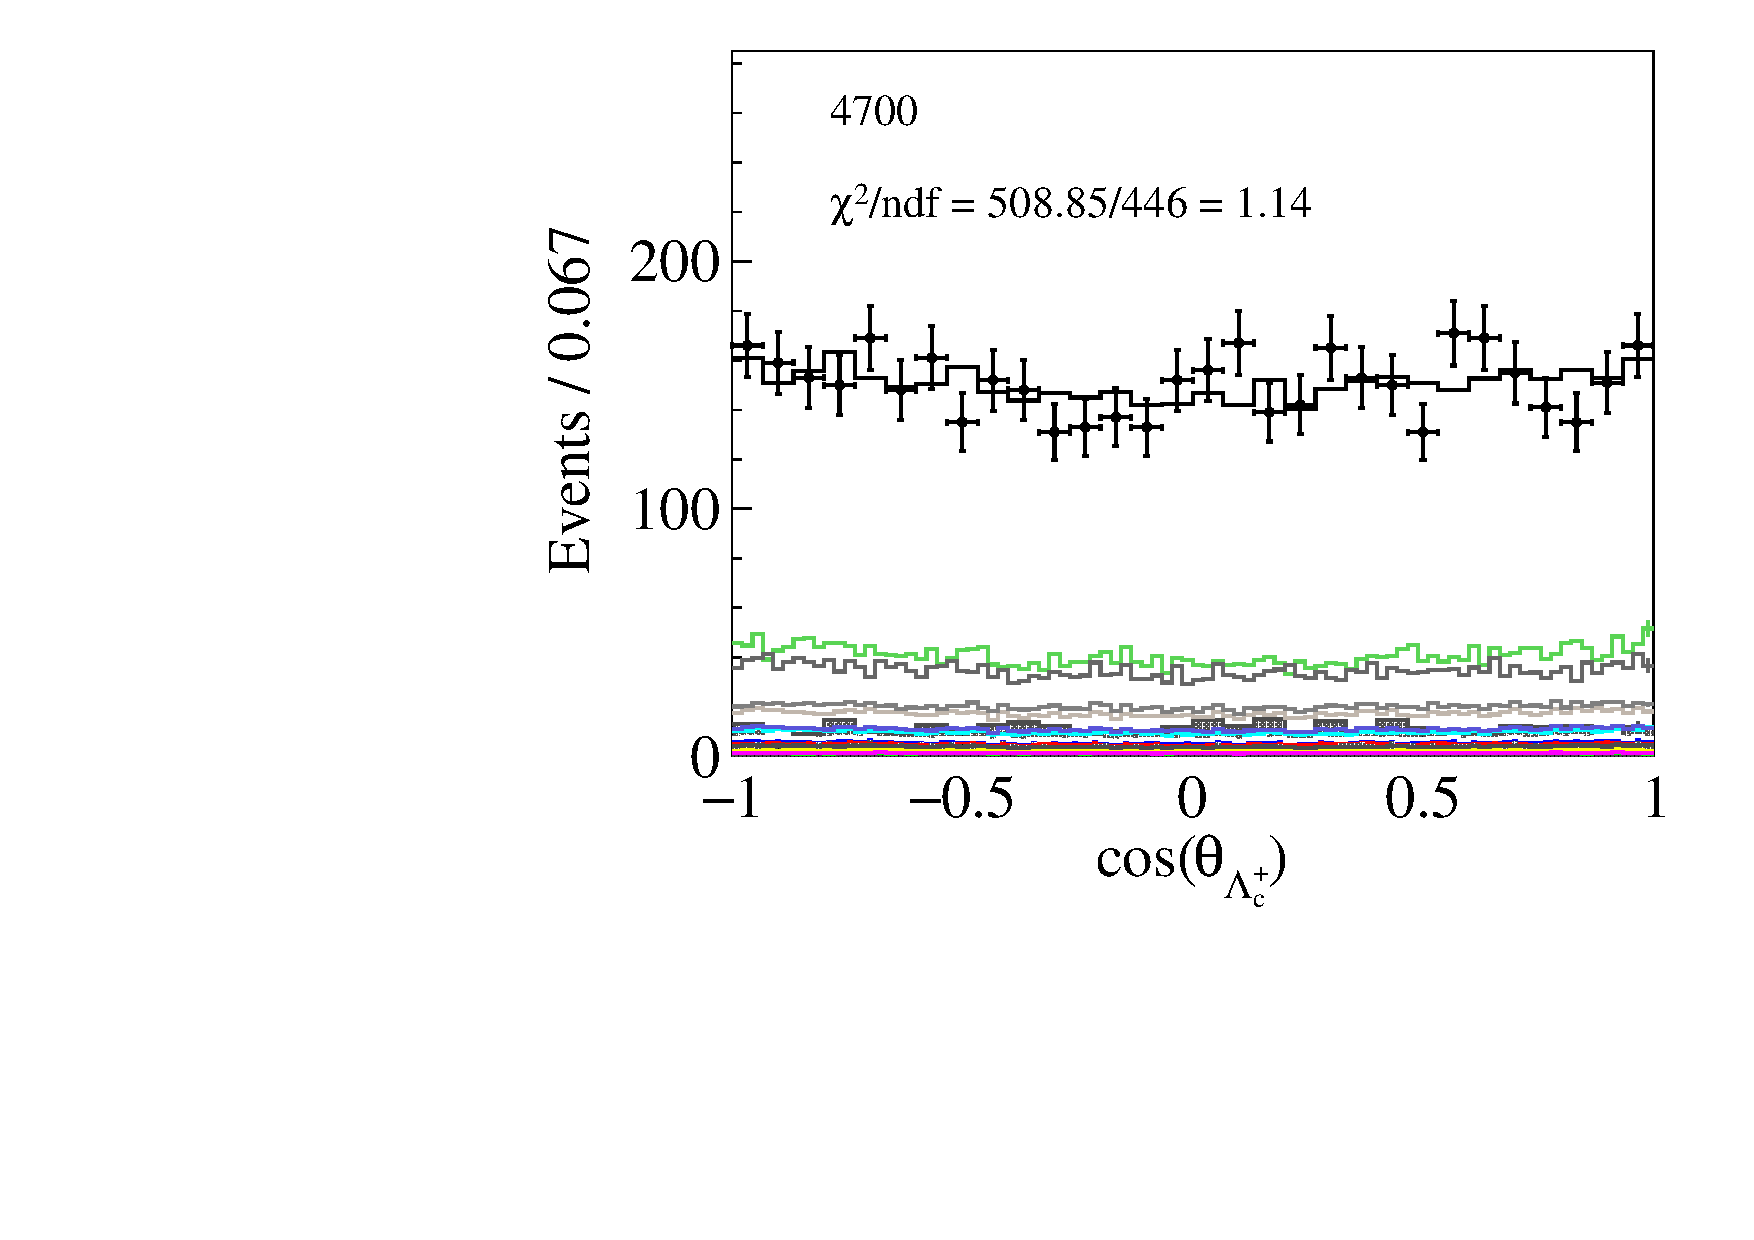
\includegraphics[width=0.24\textwidth]{figure/pwa_nominal/s6_epemDSID_Lmdc_cos_beta.pdf} \\
    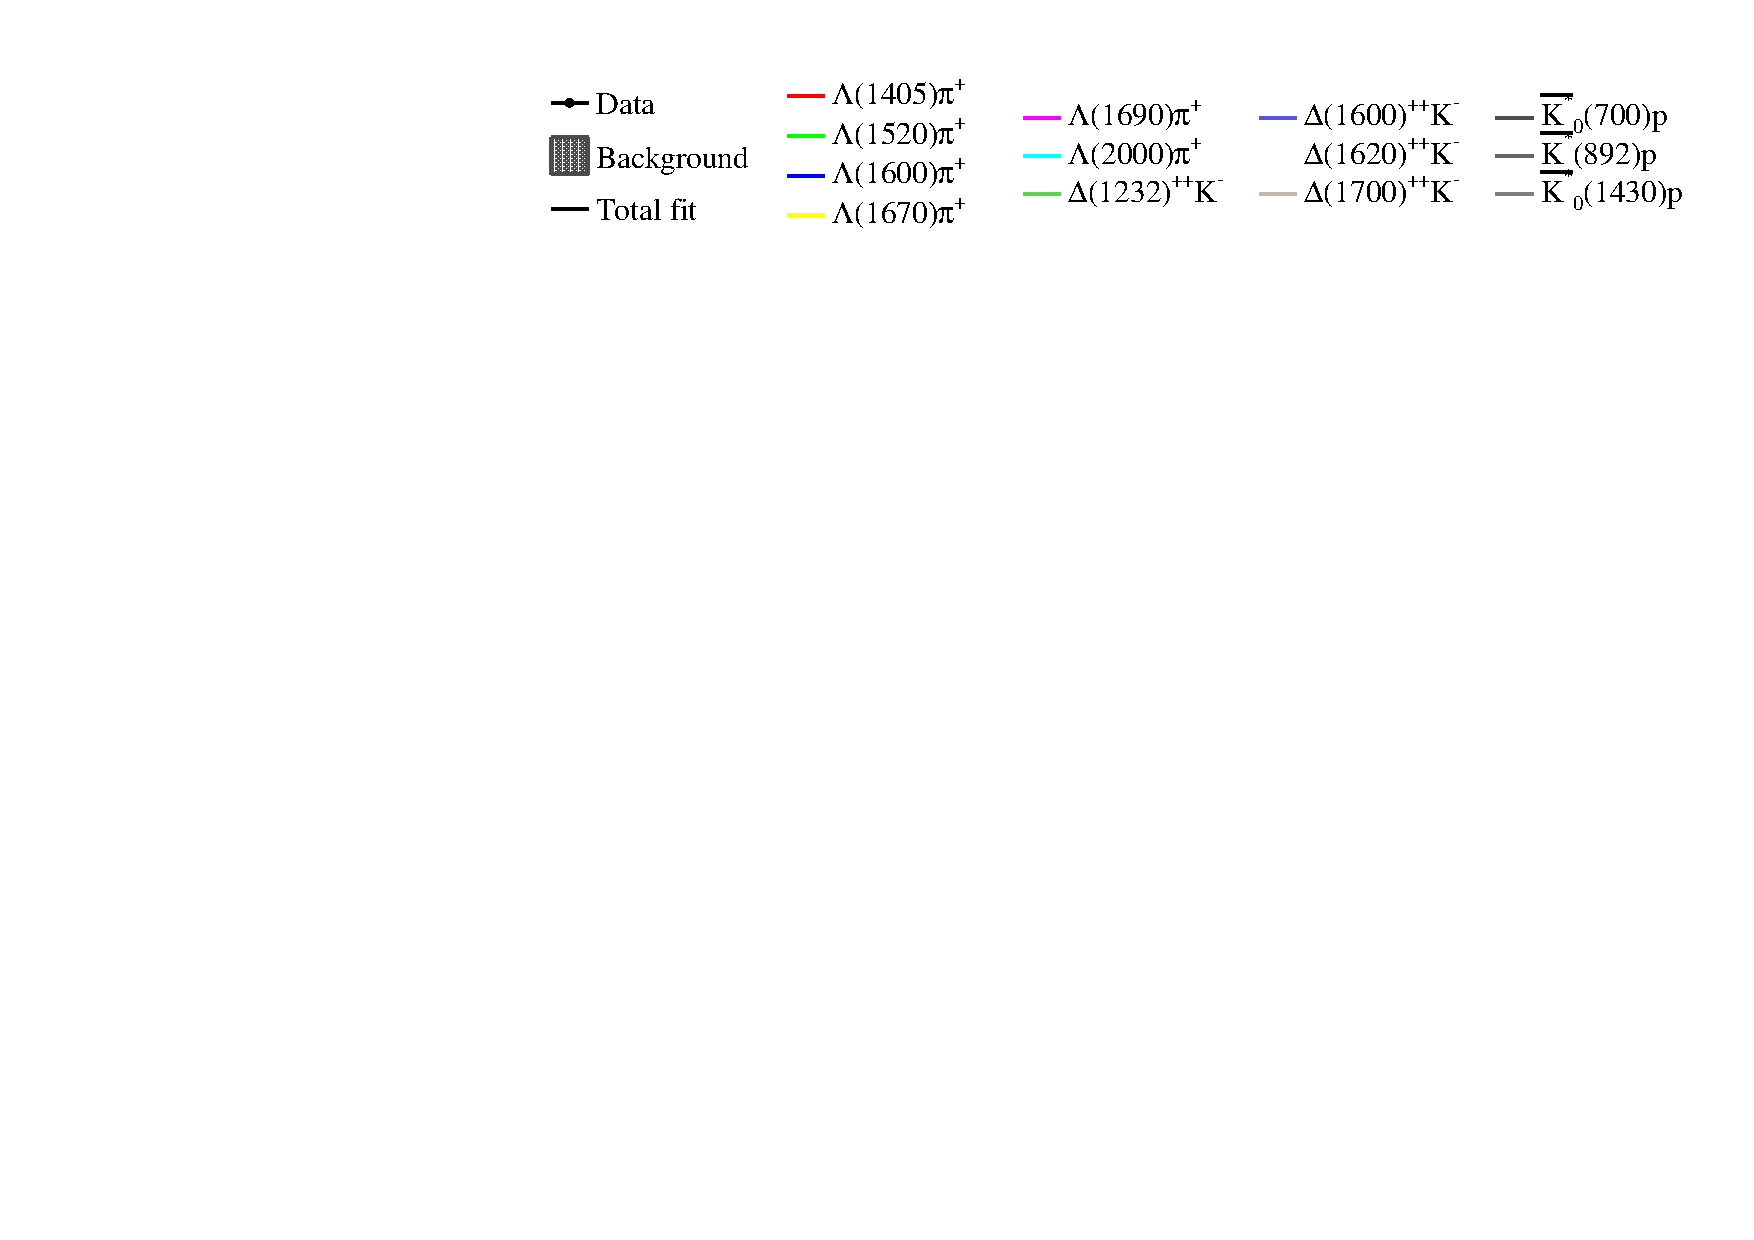
\includegraphics[width=0.80\textwidth]{figure/pwa_nominal/legend.pdf}

    \caption{Fit results of projected distributions of $M(pK^-)$, $M(p\pi^+)$, $M(K^-\pi^+)$  and helicity angle $\cos(\theta_{\lcp}^{\gamma^*})$ for energy points below $\sqrt{s} = 4.740\gev/c^2$. }
\label{fig:pwa_fit_mass_0}
\end{figure}

\begin{figure}[htbp]\centering
    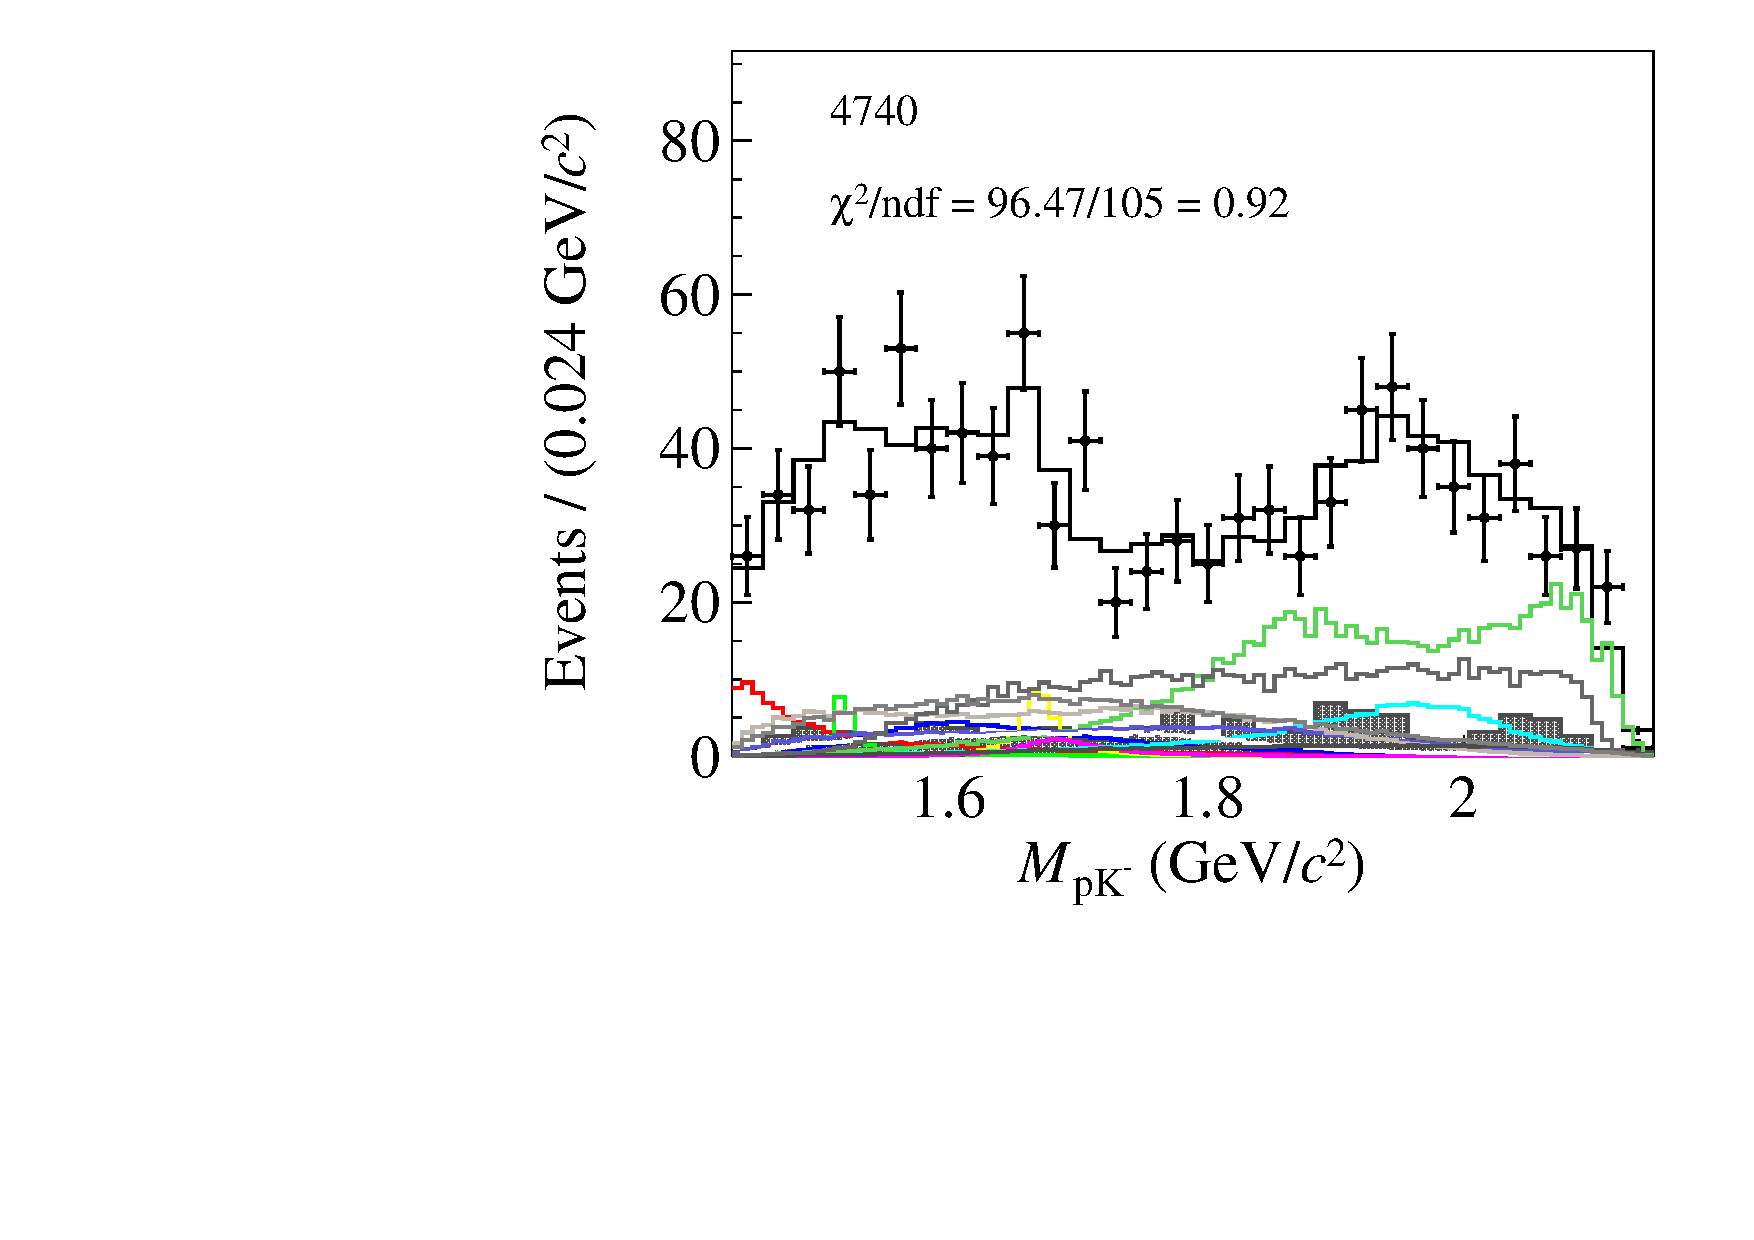
\includegraphics[width=0.24\textwidth]{figure/pwa_nominal/s7_m_R_BC.pdf}
    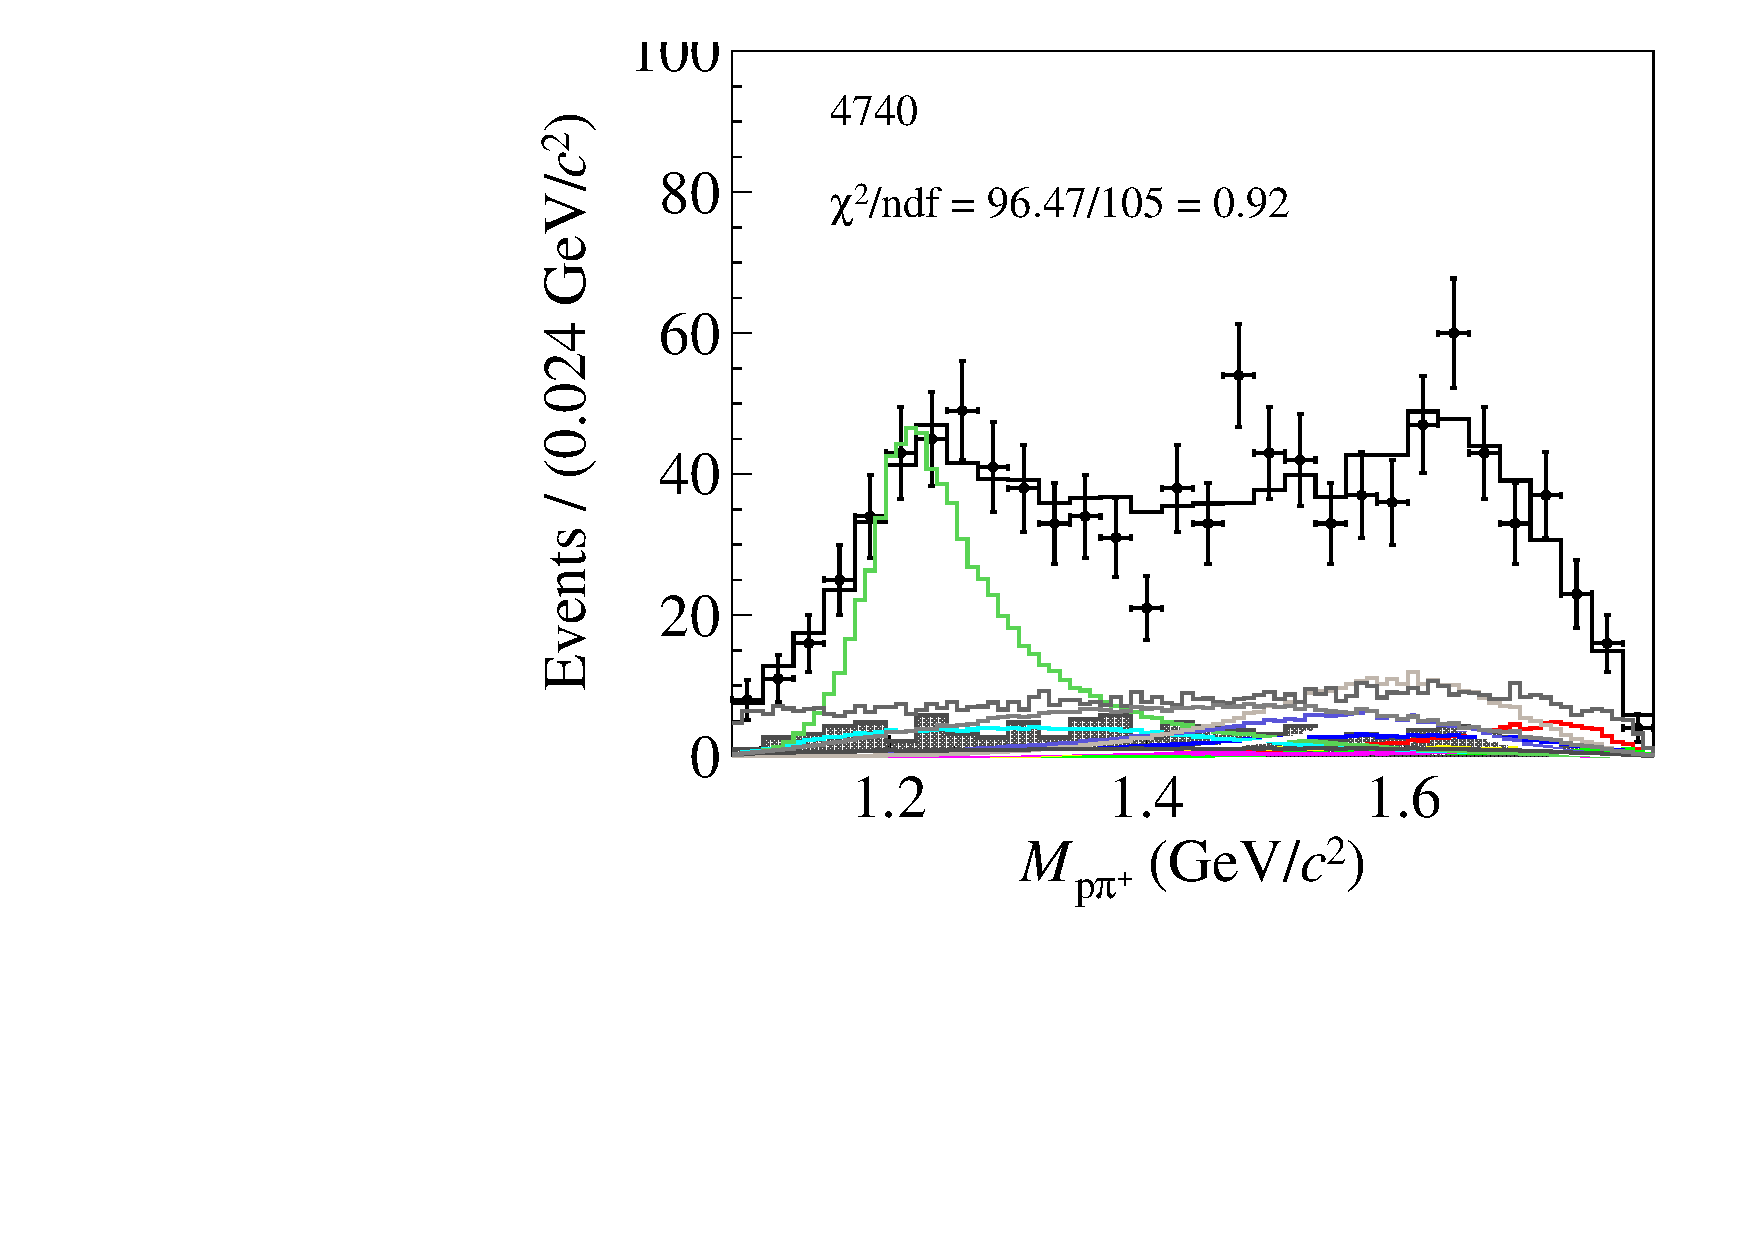
\includegraphics[width=0.24\textwidth]{figure/pwa_nominal/s7_m_R_BD.pdf}
    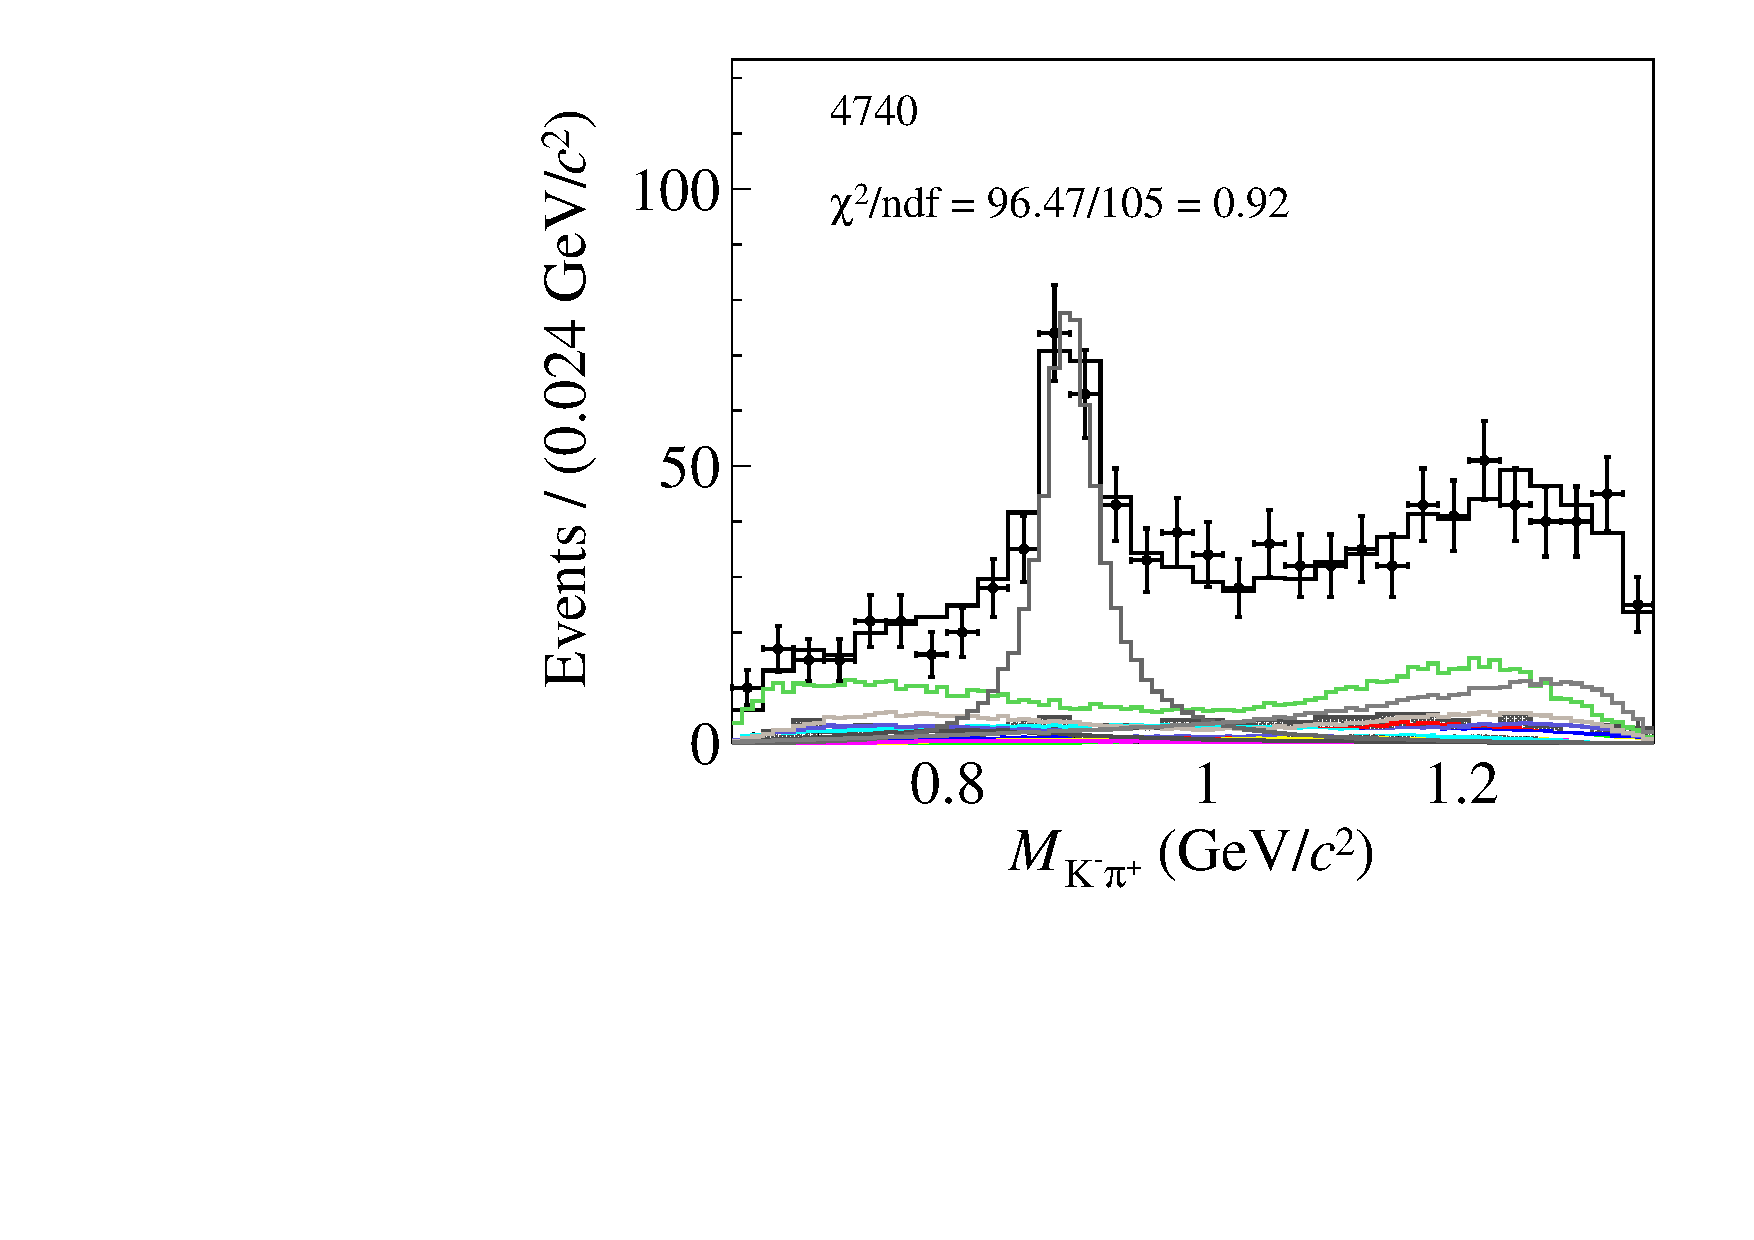
\includegraphics[width=0.24\textwidth]{figure/pwa_nominal/s7_m_R_CD.pdf}
    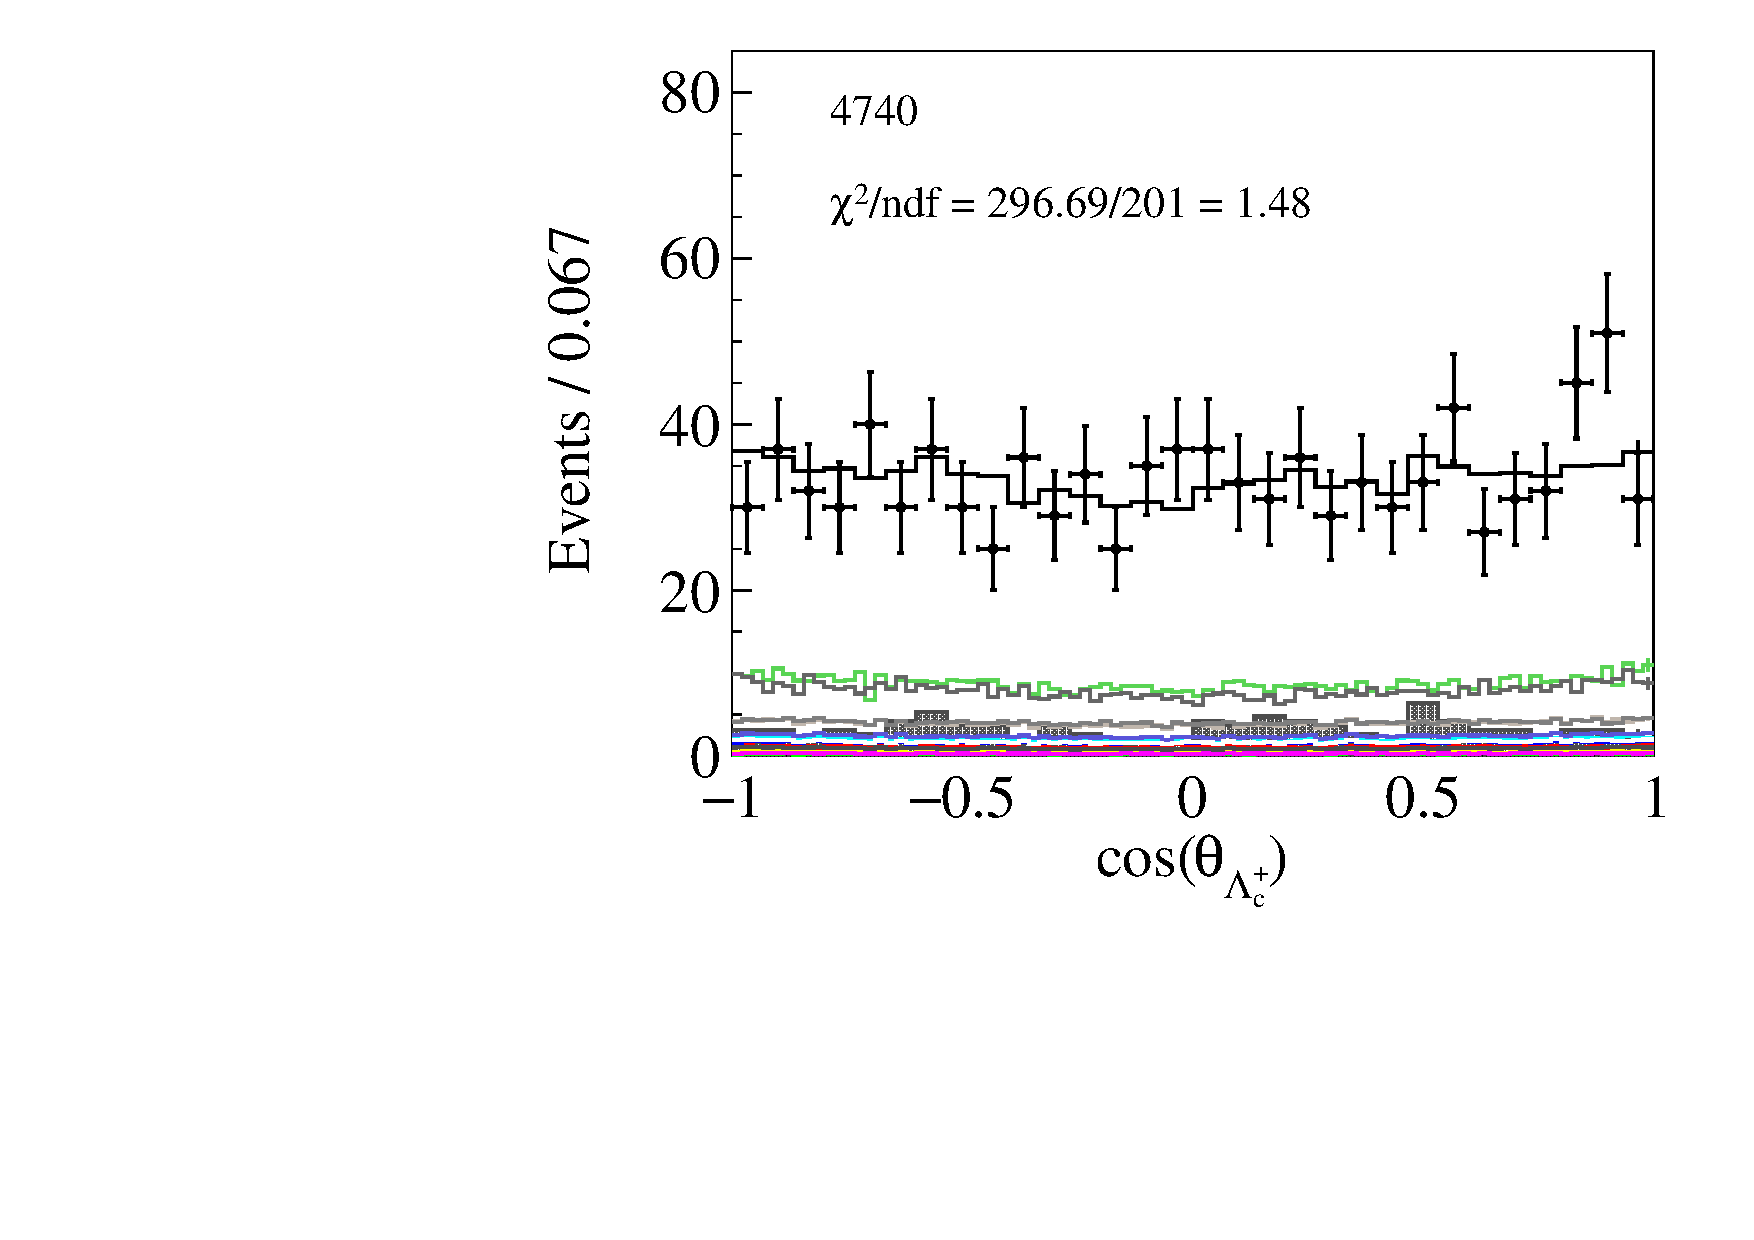
\includegraphics[width=0.24\textwidth]{figure/pwa_nominal/s7_epemDSID_Lmdc_cos_beta.pdf} \\
    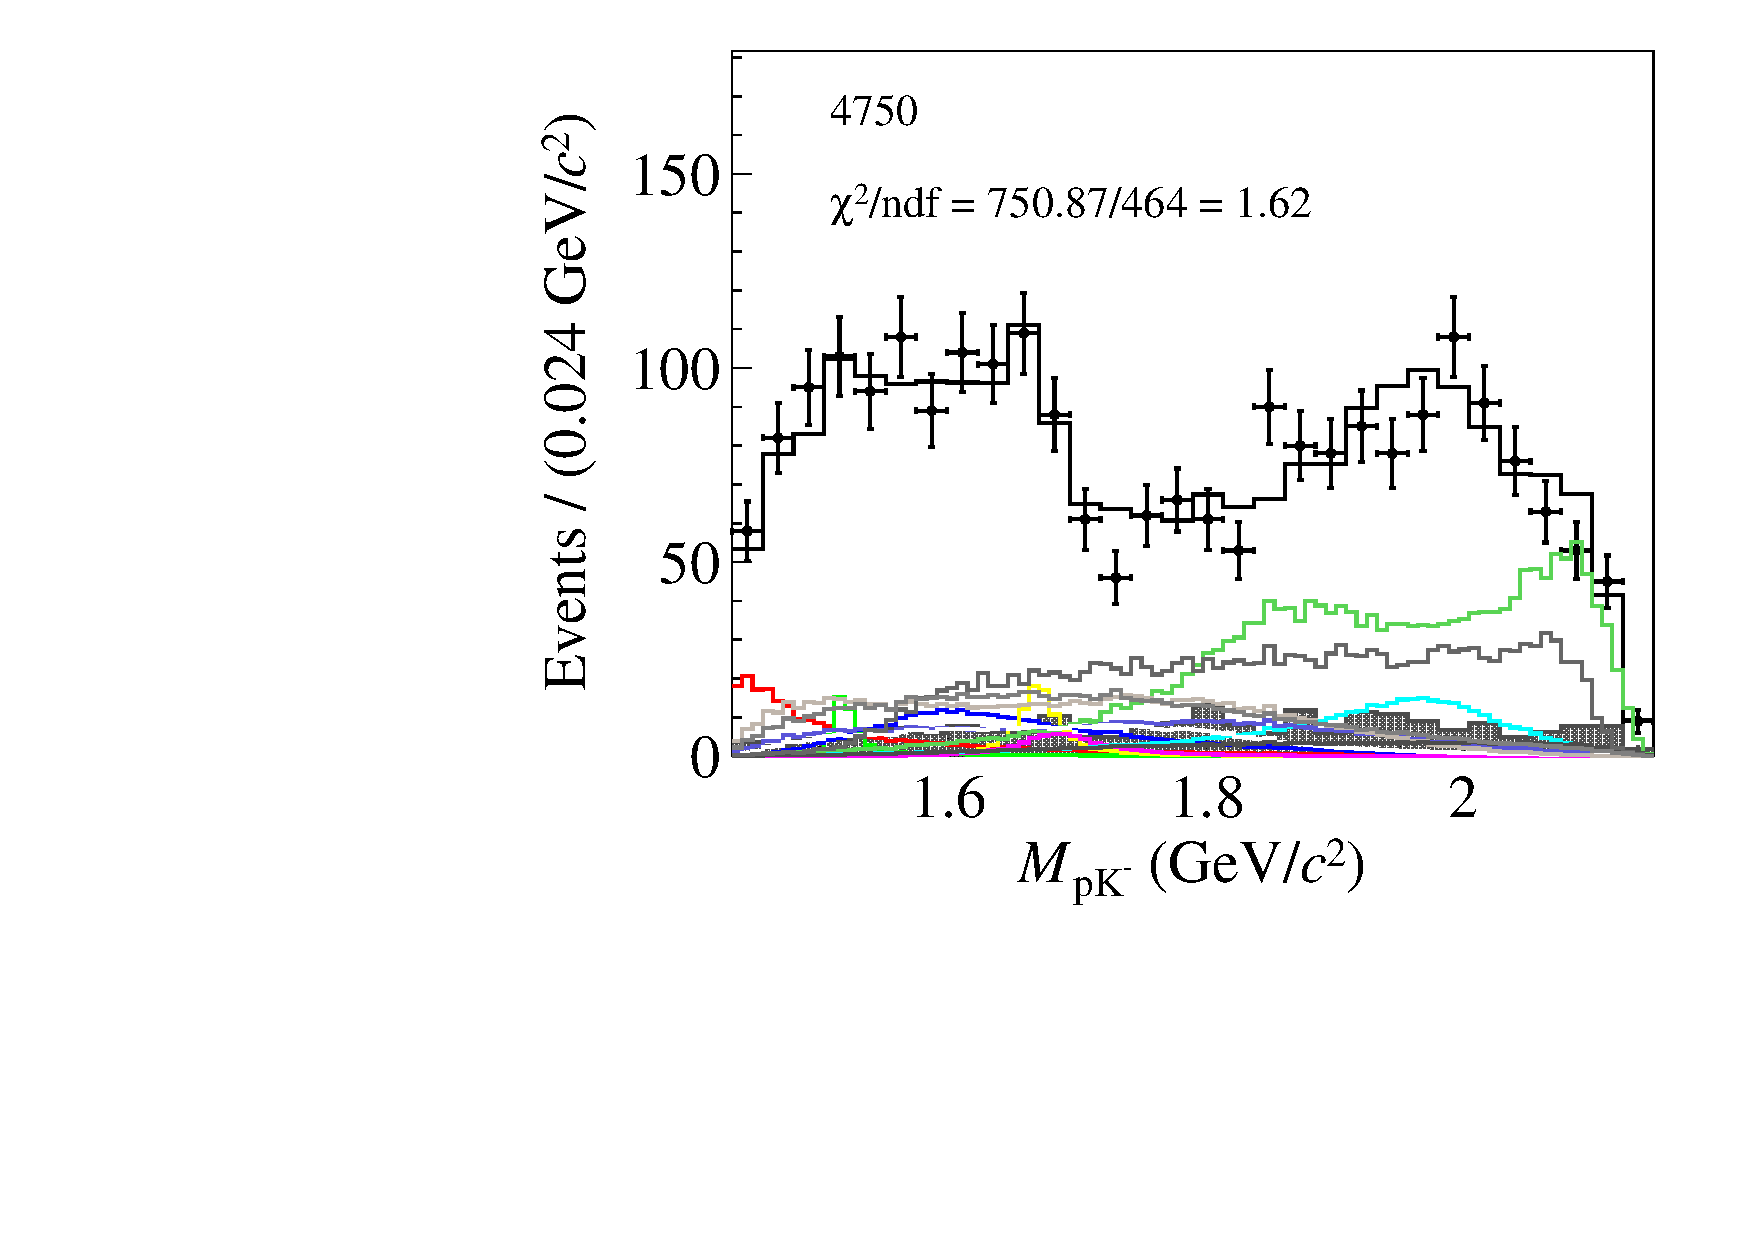
\includegraphics[width=0.24\textwidth]{figure/pwa_nominal/s8_m_R_BC.pdf}
    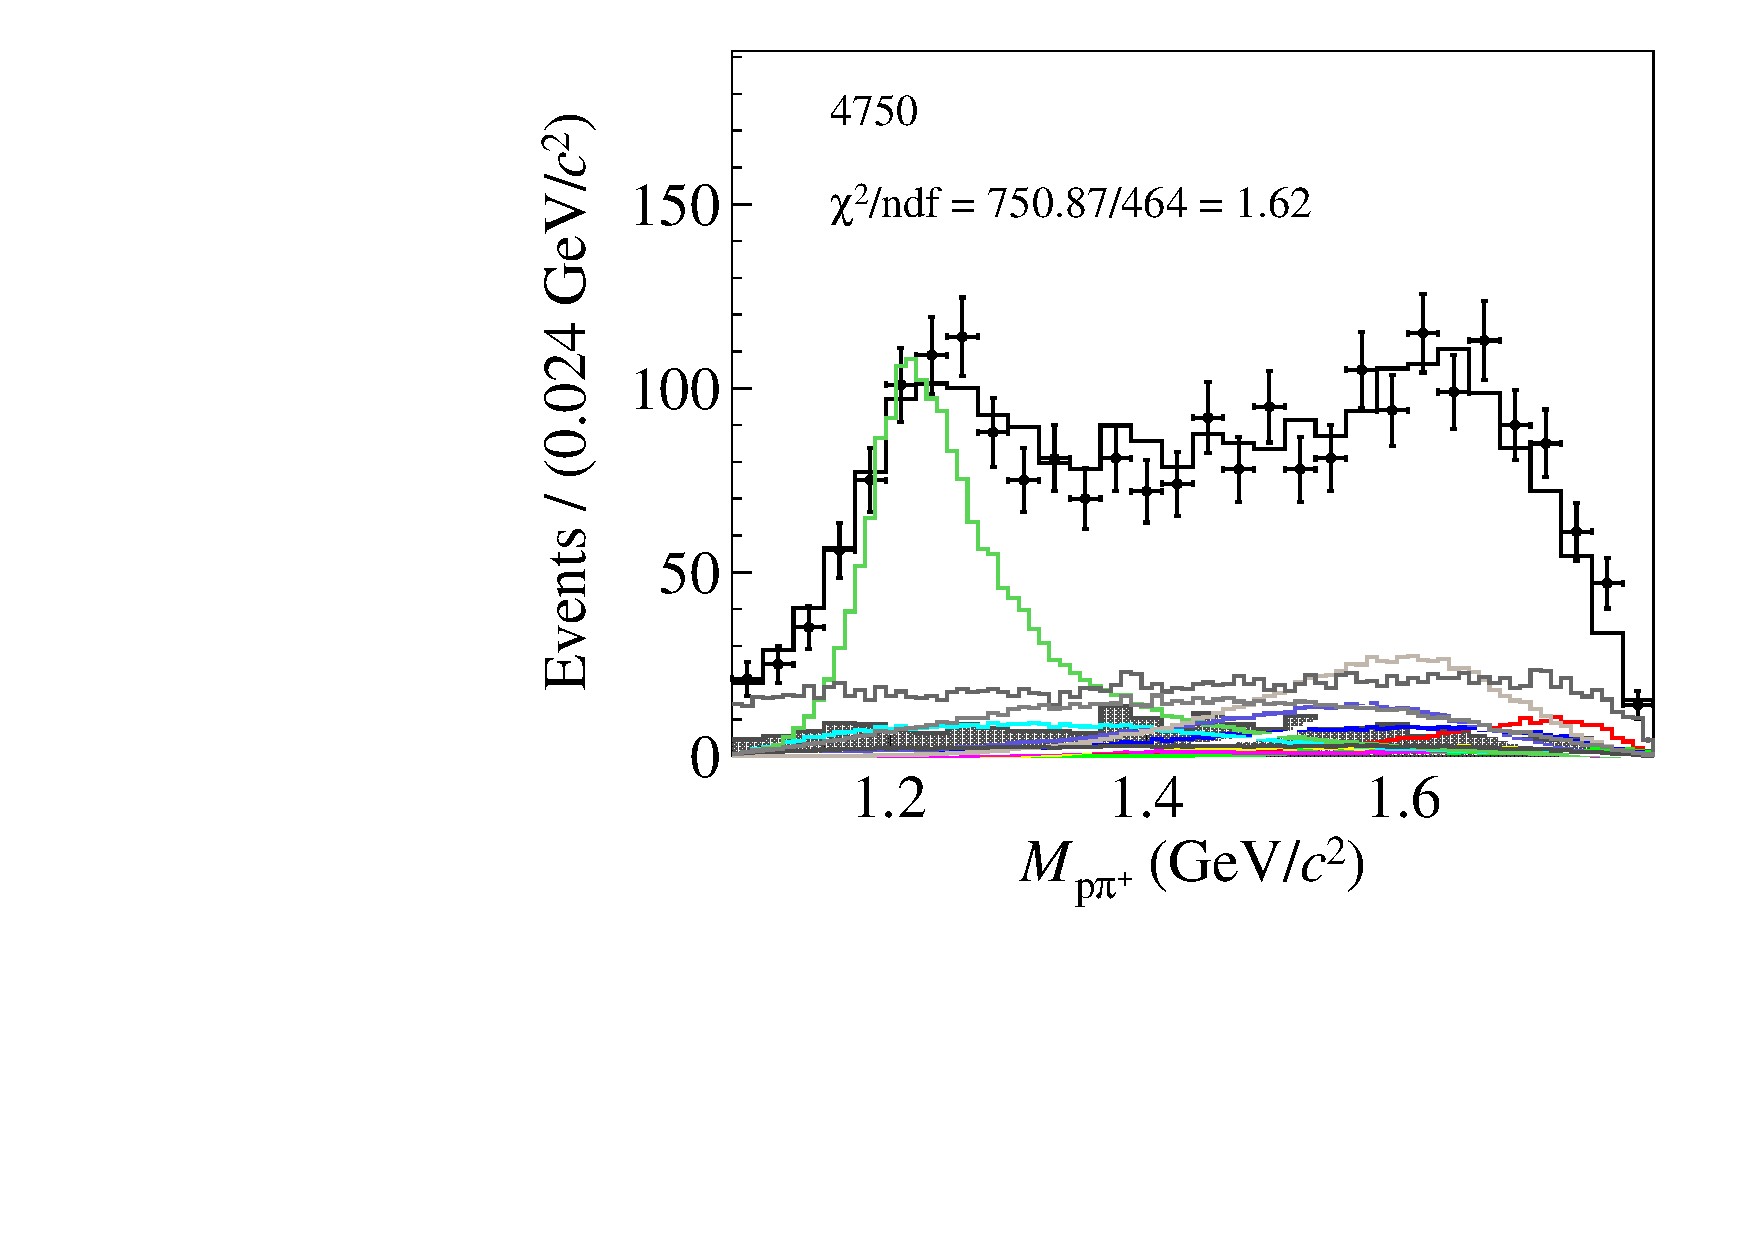
\includegraphics[width=0.24\textwidth]{figure/pwa_nominal/s8_m_R_BD.pdf}
    \includegraphics[width=0.24\textwidth]{figure/pwa_nominal/s8_m_R_CD.pdf}
    \includegraphics[width=0.24\textwidth]{figure/pwa_nominal/s8_epemDSID_Lmdc_cos_beta.pdf} \\
    \includegraphics[width=0.24\textwidth]{figure/pwa_nominal/s9_m_R_BC.pdf}
    \includegraphics[width=0.24\textwidth]{figure/pwa_nominal/s9_m_R_BD.pdf}
    \includegraphics[width=0.24\textwidth]{figure/pwa_nominal/s9_m_R_CD.pdf}
    \includegraphics[width=0.24\textwidth]{figure/pwa_nominal/s9_epemDSID_Lmdc_cos_beta.pdf} \\
    \includegraphics[width=0.24\textwidth]{figure/pwa_nominal/s10_m_R_BC.pdf}
    \includegraphics[width=0.24\textwidth]{figure/pwa_nominal/s10_m_R_BD.pdf}
    \includegraphics[width=0.24\textwidth]{figure/pwa_nominal/s10_m_R_CD.pdf}
    \includegraphics[width=0.24\textwidth]{figure/pwa_nominal/s10_epemDSID_Lmdc_cos_beta.pdf} \\
    \includegraphics[width=0.24\textwidth]{figure/pwa_nominal/s11_m_R_BC.pdf}
    \includegraphics[width=0.24\textwidth]{figure/pwa_nominal/s11_m_R_BD.pdf}
    \includegraphics[width=0.24\textwidth]{figure/pwa_nominal/s11_m_R_CD.pdf}
    \includegraphics[width=0.24\textwidth]{figure/pwa_nominal/s11_epemDSID_Lmdc_cos_beta.pdf} \\
    \includegraphics[width=0.24\textwidth]{figure/pwa_nominal/s12_m_R_BC.pdf}
    \includegraphics[width=0.24\textwidth]{figure/pwa_nominal/s12_m_R_BD.pdf}
    \includegraphics[width=0.24\textwidth]{figure/pwa_nominal/s12_m_R_CD.pdf}
    \includegraphics[width=0.24\textwidth]{figure/pwa_nominal/s12_epemDSID_Lmdc_cos_beta.pdf} \\
    \includegraphics[width=0.80\textwidth]{figure/pwa_nominal/legend.pdf}

    \caption{Fit results of projected distributions of $M(pK^-)$, $M(p\pi^+)$, $M(K^-\pi^+)$  and helicity angle $\cos(\theta_{\lcp}^{\gamma^*})$ for energy points above $\sqrt{s} = 4.700\gev/c^2$. }
\label{fig:pwa_fit_mass_1}
\end{figure}



\begin{table}[H]
    \centering
    \caption{FFs of each component and the interference at $\sqrt{s}=4.682\gev/c^2$. (I): $\Delta(1232)^{++}$, (II): $\Delta(1600)^{++}$, (III): $\Delta(1620)^{++}$, (IV): $\Delta(1700)^{++}$, (V): $\overline{K}^*_0(1430)$, (VI): $\overline{K}^*_0(700)$, (VII): $\overline{K}^*(892)$, (VIII): $\Lambda(1405)$, (IX): $\Lambda(1520)$, (X): $\Lambda(1600)$, (XI): $\Lambda(1670)$, (XII): $\Lambda(1690)$, (XIII): $\Lambda(2000)$. The total FF is 114.53$\pm$4.67\%. Only statistical uncertainties are considered.}
    \label{tab:ff_s6}
    \resizebox{1.0\textwidth}{!}{
    \begin{tabular}{cccccccccccccc}
        \hline\hline
        - & I & II & III & IV & V & VI & VII & VIII & IX & X & XI & XII & XIII\\
    I & 27.46 $\pm$ 1.03 & - & - & - & - & - & - & - & - & - & - & - & -\\
    II & -9.07 $\pm$ 2.14 & 7.69 $\pm$ 2.01 & - & - & - & - & - & - & - & - & - & - & -\\
    III & -0.00 $\pm$ 0.00 & -0.01 $\pm$ 0.00 & 5.42 $\pm$ 1.88 & - & - & - & - & - & - & - & - & - & -\\
    IV & -0.00 $\pm$ 0.00 & 0.00 $\pm$ 0.00 & 0.01 $\pm$ 0.00 & 12.73 $\pm$ 1.41 & - & - & - & - & - & - & - & - & -\\
    V & 6.32 $\pm$ 0.79 & -1.24 $\pm$ 0.82 & -1.81 $\pm$ 0.78 & -1.84 $\pm$ 1.04 & 13.69 $\pm$ 2.61 & - & - & - & - & - & - & - & -\\
    VI & 0.31 $\pm$ 0.58 & -0.54 $\pm$ 0.79 & -2.13 $\pm$ 0.59 & -2.40 $\pm$ 0.69 & 0.49 $\pm$ 1.14 & 2.91 $\pm$ 0.67 & - & - & - & - & - & - & -\\
    VII & -1.31 $\pm$ 0.45 & 1.67 $\pm$ 0.51 & -0.48 $\pm$ 0.53 & -1.31 $\pm$ 0.55 & -0.01 $\pm$ 0.00 & 0.00 $\pm$ 0.00 & 24.93 $\pm$ 0.99 & - & - & - & - & - & -\\
    VIII & -0.58 $\pm$ 0.56 & 1.59 $\pm$ 0.48 & -0.34 $\pm$ 1.12 & 0.68 $\pm$ 0.68 & -0.00 $\pm$ 2.02 & 1.39 $\pm$ 0.69 & -1.16 $\pm$ 0.60 & 4.34 $\pm$ 1.08 & - & - & - & - & -\\
    IX & 0.03 $\pm$ 0.15 & 0.47 $\pm$ 0.16 & 0.34 $\pm$ 0.09 & -0.12 $\pm$ 0.04 & 0.31 $\pm$ 0.18 & 0.14 $\pm$ 0.05 & -0.35 $\pm$ 0.10 & 0.00 $\pm$ 0.00 & 1.10 $\pm$ 0.17 & - & - & - & -\\
    X & -3.63 $\pm$ 0.60 & 1.15 $\pm$ 0.51 & 1.22 $\pm$ 0.63 & -0.64 $\pm$ 0.18 & -4.19 $\pm$ 1.13 & -0.74 $\pm$ 0.40 & -1.16 $\pm$ 0.50 & 0.01 $\pm$ 0.00 & 0.00 $\pm$ 0.00 & 5.56 $\pm$ 1.15 & - & - & -\\
    XI & -0.03 $\pm$ 0.07 & 0.08 $\pm$ 0.07 & -0.02 $\pm$ 0.09 & 0.43 $\pm$ 0.11 & 0.22 $\pm$ 0.32 & 0.39 $\pm$ 0.07 & -0.33 $\pm$ 0.05 & 1.07 $\pm$ 0.19 & 0.00 $\pm$ 0.00 & 0.00 $\pm$ 0.00 & 1.67 $\pm$ 0.26 & - & -\\
    XII & -0.09 $\pm$ 0.18 & 0.77 $\pm$ 0.23 & 0.08 $\pm$ 0.06 & -0.03 $\pm$ 0.06 & -0.12 $\pm$ 0.16 & 0.13 $\pm$ 0.04 & -0.31 $\pm$ 0.16 & -0.00 $\pm$ 0.00 & 0.26 $\pm$ 0.09 & 0.00 $\pm$ 0.00 & -0.00 $\pm$ 0.00 & 1.07 $\pm$ 0.26 & -\\
    XIII & 0.01 $\pm$ 0.16 & -0.01 $\pm$ 0.21 & -0.33 $\pm$ 0.25 & -0.45 $\pm$ 0.20 & -2.99 $\pm$ 0.72 & 2.14 $\pm$ 0.28 & -0.42 $\pm$ 0.33 & 3.27 $\pm$ 0.85 & 0.00 $\pm$ 0.00 & 0.00 $\pm$ 0.00 & 0.65 $\pm$ 0.20 & 0.00 $\pm$ 0.00 & 5.95 $\pm$ 0.51\\
    \hline\hline
    \end{tabular}}
\end{table}

\begin{table}[H]
    \centering
    \caption{FFs of each component for all energy points. (I): $\Delta(1232)^{++}$, (II): $\Delta(1600)^{++}$, (III): $\Delta(1620)^{++}$, (IV): $\Delta(1700)^{++}$, (V): $\overline{K}^*_0(1430)$, (VI): $\overline{K}^*_0(700)$, (VII): $\overline{K}^*(892)$, (VIII): $\Lambda(1405)$, (IX): $\Lambda(1520)$, (X): $\Lambda(1600)$, (XI): $\Lambda(1670)$, (XII): $\Lambda(1690)$, (XIII): $\Lambda(2000)$. The total FF is 114.23\%. Only statistical uncertainties are considered.}
    \label{tab:ff_full}
    \resizebox{1.0\textwidth}{!}{
    \begin{tabular}{ccccccccccccccc}
        \hline\hline
        dataset & I & II & III & IV & V & VI & VII & VIII & IX & X & XI & XII & XIII & Total\\\hline
        4600 & 27.32 $\pm$ 1.03 & 7.69 $\pm$ 2.01 & 5.43 $\pm$ 1.88 & 12.77 $\pm$ 1.41 & 13.67 $\pm$ 2.61 & 2.90 $\pm$ 0.67 & 24.96 $\pm$ 0.98 & 4.34 $\pm$ 1.08 & 1.11 $\pm$ 0.17 & 5.56 $\pm$ 1.15 & 1.68 $\pm$ 0.26 & 1.07 $\pm$ 0.26 & 5.93 $\pm$ 0.51 & 114.43 $\pm$ 4.67 \\
        4612 & 27.28 $\pm$ 1.03 & 7.67 $\pm$ 2.01 & 5.42 $\pm$ 1.88 & 12.73 $\pm$ 1.41 & 13.65 $\pm$ 2.60 & 2.90 $\pm$ 0.66 & 25.01 $\pm$ 0.99 & 4.36 $\pm$ 1.08 & 1.09 $\pm$ 0.17 & 5.56 $\pm$ 1.15 & 1.69 $\pm$ 0.26 & 1.07 $\pm$ 0.26 & 5.93 $\pm$ 0.51 & 114.37 $\pm$ 4.66 \\
        4626 & 27.24 $\pm$ 1.02 & 7.68 $\pm$ 2.01 & 5.42 $\pm$ 1.88 & 12.74 $\pm$ 1.41 & 13.66 $\pm$ 2.60 & 2.90 $\pm$ 0.67 & 25.10 $\pm$ 0.99 & 4.34 $\pm$ 1.08 & 1.11 $\pm$ 0.17 & 5.56 $\pm$ 1.15 & 1.68 $\pm$ 0.26 & 1.07 $\pm$ 0.26 & 5.94 $\pm$ 0.51 & 114.44 $\pm$ 4.66 \\
        4640 & 27.34 $\pm$ 1.03 & 7.68 $\pm$ 2.01 & 5.42 $\pm$ 1.88 & 12.74 $\pm$ 1.41 & 13.67 $\pm$ 2.61 & 2.91 $\pm$ 0.67 & 24.88 $\pm$ 0.98 & 4.36 $\pm$ 1.08 & 1.10 $\pm$ 0.17 & 5.54 $\pm$ 1.15 & 1.67 $\pm$ 0.26 & 1.07 $\pm$ 0.26 & 5.95 $\pm$ 0.51 & 114.34 $\pm$ 4.66 \\
        4660 & 27.27 $\pm$ 1.03 & 7.68 $\pm$ 2.01 & 5.41 $\pm$ 1.88 & 12.72 $\pm$ 1.41 & 13.68 $\pm$ 2.61 & 2.90 $\pm$ 0.67 & 24.99 $\pm$ 0.99 & 4.33 $\pm$ 1.08 & 1.11 $\pm$ 0.17 & 5.56 $\pm$ 1.15 & 1.69 $\pm$ 0.26 & 1.08 $\pm$ 0.26 & 5.95 $\pm$ 0.51 & 114.37 $\pm$ 4.66 \\
        4680 & 27.46 $\pm$ 1.03 & 7.69 $\pm$ 2.01 & 5.42 $\pm$ 1.88 & 12.73 $\pm$ 1.41 & 13.69 $\pm$ 2.61 & 2.91 $\pm$ 0.67 & 24.93 $\pm$ 0.99 & 4.34 $\pm$ 1.08 & 1.10 $\pm$ 0.17 & 5.56 $\pm$ 1.15 & 1.67 $\pm$ 0.26 & 1.07 $\pm$ 0.26 & 5.95 $\pm$ 0.51 & 114.53 $\pm$ 4.67 \\
        4700 & 27.35 $\pm$ 1.03 & 7.67 $\pm$ 2.01 & 5.43 $\pm$ 1.88 & 12.74 $\pm$ 1.41 & 13.67 $\pm$ 2.61 & 2.90 $\pm$ 0.66 & 24.93 $\pm$ 0.98 & 4.36 $\pm$ 1.08 & 1.10 $\pm$ 0.17 & 5.57 $\pm$ 1.15 & 1.69 $\pm$ 0.26 & 1.08 $\pm$ 0.26 & 5.93 $\pm$ 0.51 & 114.42 $\pm$ 4.66 \\
        4740 & 27.50 $\pm$ 1.03 & 7.68 $\pm$ 2.01 & 5.42 $\pm$ 1.88 & 12.72 $\pm$ 1.41 & 13.66 $\pm$ 2.60 & 2.90 $\pm$ 0.67 & 25.00 $\pm$ 0.99 & 4.36 $\pm$ 1.08 & 1.10 $\pm$ 0.17 & 5.55 $\pm$ 1.15 & 1.68 $\pm$ 0.26 & 1.07 $\pm$ 0.26 & 5.96 $\pm$ 0.51 & 114.59 $\pm$ 4.66 \\
        4750 & 27.34 $\pm$ 1.03 & 7.70 $\pm$ 2.02 & 5.44 $\pm$ 1.89 & 12.78 $\pm$ 1.41 & 13.69 $\pm$ 2.61 & 2.91 $\pm$ 0.67 & 25.00 $\pm$ 0.99 & 4.35 $\pm$ 1.08 & 1.10 $\pm$ 0.17 & 5.56 $\pm$ 1.15 & 1.68 $\pm$ 0.26 & 1.08 $\pm$ 0.26 & 5.94 $\pm$ 0.51 & 114.57 $\pm$ 4.67 \\
        4780 & 27.40 $\pm$ 1.03 & 7.67 $\pm$ 2.01 & 5.41 $\pm$ 1.88 & 12.70 $\pm$ 1.41 & 13.65 $\pm$ 2.60 & 2.91 $\pm$ 0.67 & 24.99 $\pm$ 0.98 & 4.34 $\pm$ 1.08 & 1.09 $\pm$ 0.17 & 5.54 $\pm$ 1.15 & 1.68 $\pm$ 0.26 & 1.07 $\pm$ 0.26 & 5.95 $\pm$ 0.51 & 114.40 $\pm$ 4.66 \\
        4840 & 27.47 $\pm$ 1.03 & 7.67 $\pm$ 2.01 & 5.41 $\pm$ 1.88 & 12.71 $\pm$ 1.41 & 13.66 $\pm$ 2.60 & 2.91 $\pm$ 0.67 & 25.11 $\pm$ 0.99 & 4.32 $\pm$ 1.07 & 1.09 $\pm$ 0.17 & 5.55 $\pm$ 1.15 & 1.68 $\pm$ 0.26 & 1.07 $\pm$ 0.26 & 5.95 $\pm$ 0.51 & 114.61 $\pm$ 4.66 \\
        4920 & 27.21 $\pm$ 1.02 & 7.70 $\pm$ 2.02 & 5.43 $\pm$ 1.89 & 12.79 $\pm$ 1.42 & 13.66 $\pm$ 2.60 & 2.90 $\pm$ 0.67 & 24.95 $\pm$ 0.98 & 4.39 $\pm$ 1.09 & 1.11 $\pm$ 0.17 & 5.56 $\pm$ 1.15 & 1.69 $\pm$ 0.26 & 1.08 $\pm$ 0.26 & 5.92 $\pm$ 0.51 & 114.40 $\pm$ 4.67 \\
        4950 & 27.27 $\pm$ 1.03 & 7.68 $\pm$ 2.01 & 5.43 $\pm$ 1.88 & 12.74 $\pm$ 1.41 & 13.68 $\pm$ 2.61 & 2.89 $\pm$ 0.66 & 24.95 $\pm$ 0.98 & 4.36 $\pm$ 1.08 & 1.12 $\pm$ 0.17 & 5.57 $\pm$ 1.15 & 1.69 $\pm$ 0.26 & 1.07 $\pm$ 0.26 & 5.94 $\pm$ 0.51 & 114.37 $\pm$ 4.66 \\
        Combined  & 27.34 $\pm$ 1.03 & 7.68 $\pm$ 2.02 & 5.42 $\pm$ 1.89 & 12.74 $\pm$ 1.42 & 13.67 $\pm$ 2.61 & 2.90 $\pm$ 0.67 & 24.98 $\pm$ 0.99 & 4.35 $\pm$ 1.09 & 1.10 $\pm$ 0.17 & 5.56 $\pm$ 1.15 & 1.68 $\pm$ 0.26 & 1.07 $\pm$ 0.26 & 5.94 $\pm$ 0.51 & 114.45 $\pm$ 4.67\\
       
    \hline\hline
    \end{tabular}}
\end{table}

\begin{table}[H]
    \centering
    \caption{The partial wave amplitudes ($g_{ls}^{\gamma^*}$) and derived $\alpha_0$ and $\sin\Delta_0$ for each energy point. Only statistical uncertainties are considered.}
    \label{tab:fit_polarization}
    \resizebox{0.9\textwidth}{!}{
    \begin{tabular}{ccccc}
        \hline\hline
    dataset & $g_{2,1}^{\gamma^*}$ magnitude & $g_{2,1}^{\gamma^*}$ phase & $\alpha_0$ & $\sin\Delta_0$ \\\hline
    4600 & 0.17 $\pm$ 0.03 & -2.39 $\pm$ 0.22 & -0.25 $\pm$ 0.04 & -0.22 $\pm$ 0.08 \\
    4612 & 0.27 $\pm$ 0.11 & -1.98 $\pm$ 0.29 & -0.24 $\pm$ 0.09 & -0.46 $\pm$ 0.21 \\
    4626 & 3.55 $\pm$ 0.40 & -0.48 $\pm$ 0.18 & -0.19 $\pm$ 0.04 & -0.24 $\pm$ 0.10 \\
    4640 & 2.55 $\pm$ 0.28 & -0.67 $\pm$ 0.12 & -0.08 $\pm$ 0.05 & -0.44 $\pm$ 0.10 \\
    4660 & 0.26 $\pm$ 0.06 & -1.50 $\pm$ 0.10 & -0.01 $\pm$ 0.05 & -0.51 $\pm$ 0.10 \\
    4680 & 2.08 $\pm$ 0.12 & -0.51 $\pm$ 0.07 & 0.12 $\pm$ 0.03 & -0.43 $\pm$ 0.06 \\
    4700 & 1.57 $\pm$ 0.18 & -0.55 $\pm$ 0.12 & 0.32 $\pm$ 0.07 & -0.59 $\pm$ 0.14 \\
    4740 & 0.23 $\pm$ 0.10 & 0.50 $\pm$ 0.45 & 0.42 $\pm$ 0.16 & 0.28 $\pm$ 0.30 \\
    4750 & 1.56 $\pm$ 0.21 & -0.36 $\pm$ 0.17 & 0.42 $\pm$ 0.10 & -0.42 $\pm$ 0.21 \\
    4780 & 1.97 $\pm$ 0.24 & -0.49 $\pm$ 0.16 & 0.17 $\pm$ 0.08 & -0.43 $\pm$ 0.15 \\
    4840 & 0.25 $\pm$ 0.09 & -0.81 $\pm$ 0.25 & 0.33 $\pm$ 0.11 & -0.43 $\pm$ 0.22 \\
    4914 & 1.23 $\pm$ 0.30 & 0.20 $\pm$ 0.24 & 0.70 $\pm$ 0.20 & 0.35 $\pm$ 0.45 \\
    4946 & 1.62 $\pm$ 0.39 & -0.18 $\pm$ 0.33 & 0.45 $\pm$ 0.22 & -0.22 $\pm$ 0.40 \\
    \hline\hline
    \end{tabular}
    }
\end{table}

\subsection{Decay asymmetry parameters}
\label{sec:decay_asymmetry}
For each two-body decay of the $\lcp$, the associated decay asymmetry parameter $\alpha_R$ is measured. It characterizes the two-body decay angular distribution,
\begin{equation}
    \frac{\mathrm{d}\Gamma}{\mathrm{d}\cos\theta_R} \varpropto \frac{1}{2}(1+\alpha_R P \cos\theta_R),
\end{equation}
where $\cos\theta_R = \hat{\boldsymbol{P}} \cdot \hat{\boldsymbol{p}}(R)$ is the cosine of the angle between the polarization vector $\boldsymbol{P}$ and the direction of intermediate resonance in the $\lcp$ rest frame $\hat{\boldsymbol{p}}(R)$. The $\alpha$ parameter can be expressed as a combination of helicity coupling squared moduli. For the $\lcp$ decaying to a pair of states with spin $J$ and 0 (for $\Lambda^*$, $\Delta^{++}$ and spin-zero $\overline{K}^*$), the $\alpha_R$ can be written as
\begin{equation}
    \alpha_R = \frac{|H_{1/2,0}|^2 - |H_{-1/2,0}|^2}{|H_{1/2,0}|^2 + |H_{-1/2,0}|^2}.
\end{equation}
For $J = 1/2$ intermediate resonance states, including $\Lambda(1405)$, $\Lambda(1600)$, $\Lambda(1670)$, $\Lambda(2000)$ and $\Delta(1620)^{++}$, the helicity couplings are
\begin{equation}
    H_{ \mp\frac{1}{2}, 0 } = \frac{\sqrt{2} \left(g_{0,\frac{1}{2}} \pm g_{1,\frac{1}{2}}\right)}{2}.
\end{equation}
For $J = 3/2$ intermediate resonance states, including $\Lambda(1520)$, $\Lambda(1690)$, $\Delta(1232)^{++}$, $\Delta(1600)^{++}$, $\Delta(1700)^{++}$, the helicity couplings are
\begin{equation}
    H_{ \mp\frac{1}{2}, 0 } = \frac{\sqrt{2} \left(- g_{1,\frac{3}{2}} \mp g_{2,\frac{3}{2}}\right)}{2}.
\end{equation}
For spin-zero $\overline{K}^*$ contributions, $\overline{K}^*_0(700)$ and $\overline{K}^*_0(1430)$, the helicity couplings are
\begin{equation}
    H_{ 0, \mp\frac{1}{2} } = \frac{\sqrt{2} \left(g_{0,\frac{1}{2}} \mp g_{1,\frac{1}{2}}\right)}{2}.
\end{equation}
For the decay chain $\lcp \to \bar{K}^*(892)p$, three parameters are defined to identify the possible effects due to the parity violation in the decay~\cite{Hong:2022prk}:
\begin{equation}
    \begin{split}
    \alpha_{\bar{K}^*(892)p} = \frac{|H_{1,\frac{1}{2}}|^2 - |H_{-1,-\frac{1}{2}}|^2}{|H_{1,\frac{1}{2}}|^2 +|H_{-1,-\frac{1}{2}}|^2}, \\
    \beta_{\bar{K}^*(892)p} = \frac{|H_{0,\frac{1}{2}}|^2 - |H_{0,-\frac{1}{2}}|^2}{|H_{0,\frac{1}{2}}|^2 +|H_{0,-\frac{1}{2}}|^2}, \\
    \gamma_{\bar{K}^*(892)p} = \frac{|H_{1,\frac{1}{2}}|^2 + |H_{-1,-\frac{1}{2}}|^2}{|H_{0,\frac{1}{2}}|^2 +|H_{0,-\frac{1}{2}}|^2}.
    \end{split}
\end{equation}
The helicity couplings can be expressed using $g_{ls}$ parameters by:
\begin{equation}
    \begin{split}
        H_{ -1, \frac{-1}{2} } = - \frac{\sqrt{3} g_{0,\frac{1}{2}}}{3} - \frac{\sqrt{3} g_{1,\frac{1}{2}}}{3} - \frac{\sqrt{6} g_{1,\frac{3}{2}}}{6} - \frac{\sqrt{6} g_{2,\frac{3}{2}}}{6},\\
        H_{ 0, \frac{-1}{2} } = - \frac{\sqrt{6} g_{0,\frac{1}{2}}}{6} + \frac{\sqrt{6} g_{1,\frac{1}{2}}}{6} - \frac{\sqrt{3} g_{1,\frac{3}{2}}}{3} + \frac{\sqrt{3} g_{2,\frac{3}{2}}}{3},\\
        H_{ 0, \frac{1}{2} } = \frac{\sqrt{6} g_{0,\frac{1}{2}}}{6} + \frac{\sqrt{6} g_{1,\frac{1}{2}}}{6} - \frac{\sqrt{3} g_{1,\frac{3}{2}}}{3} - \frac{\sqrt{3} g_{2,\frac{3}{2}}}{3},\\
        H_{ 1, \frac{1}{2} } = \frac{\sqrt{3} g_{0,\frac{1}{2}}}{3} - \frac{\sqrt{3} g_{1,\frac{1}{2}}}{3} - \frac{\sqrt{6} g_{1,\frac{3}{2}}}{6} + \frac{\sqrt{6} g_{2,\frac{3}{2}}}{6}.
    \end{split}
\end{equation}
Additionally, there is another definition for the parameterization of parity asymmetry~\cite{Hrivnac:1994jx}:
\begin{equation}
    \Lambda_{\bar{K}^*(892)p} = \frac{|H_{1,\frac{1}{2}}|^2 - |H_{-1,-\frac{1}{2}}|^2 + |H_{0,\frac{1}{2}}|^2 - |H_{0,-\frac{1}{2}}|^2}{|H_{1,\frac{1}{2}}|^2 +|H_{-1,-\frac{1}{2}}|^2 + |H_{0,\frac{1}{2}}|^2 +|H_{0,-\frac{1}{2}}|^2}. 
\end{equation}
The calculated $\alpha_R$ results are listed in Table~\ref{tab:fit_asymmetry}. 

\begin{table}[h]
    \centering
    \caption{The decay asymmetry parameters ($\alpha_R$) for $\lcp$ weakly decaying to a pair of state with spin $J$ and 0. Only statistical uncertainties are considered.}
    \label{tab:fit_asymmetry}
    \begin{tabular}{cc}
        \hline\hline
    Parameters  & Results \\\hline
    $\alpha_{\Lambda_c^+}^{\pi^{+}\Lambda(1520)}$ & 0.021$\pm$0.048\\
    $\alpha_{\Lambda_c^+}^{\pi^{+}\Lambda(1690)}$ & 0.083$\pm$0.051\\
    $\alpha_{\Lambda_c^+}^{K^{-}\Delta(1232)^{++}}$ & 0.023$\pm$0.053\\
    $\alpha_{\Lambda_c^+}^{K^{-}\Delta(1600)^{++}}$ & 0.299$\pm$0.047\\
    $\alpha_{\Lambda_c^+}^{K^{-}\Delta(1700)^{++}}$ & -0.168$\pm$0.045\\
    $\alpha_{\Lambda_c^+}^{\pi^{+}\Lambda(1405)}$ & 0.113$\pm$0.049\\
    $\alpha_{\Lambda_c^+}^{\pi^{+}\Lambda(1600)}$ & 0.128$\pm$0.051\\
    $\alpha_{\Lambda_c^+}^{\pi^{+}\Lambda(1670)}$ & -0.194$\pm$0.047\\
    $\alpha_{\Lambda_c^+}^{\pi^{+}\Lambda(2000)}$ & 0.014$\pm$0.051\\
    $\alpha_{\Lambda_c^+}^{K^{-}\Delta(1620)^{++}}$ & 0.071$\pm$0.052\\
    $\alpha_{\Lambda_c^+}^{p\overline{K}^*_0(700)}$ & 0.188$\pm$0.053\\
    $\alpha_{\Lambda_c^+}^{p\overline{K}^*_0(1430)}$ & -0.079$\pm$0.053\\
    $\alpha_{\Lambda_c^+}^{p\overline{K}^*(892)}$ & 0.170$\pm$0.053\\
    $\beta_{\Lambda_c^+}^{p\overline{K}^*(892)}$ & -0.048$\pm$0.057\\
    $\gamma_{\Lambda_c^+}^{p\overline{K}^*(892)}$ & -0.149$\pm$0.049\\
    $\Lambda_{\Lambda_c^+}^{p\overline{K}^*(892)}$ & 0.151$\pm$0.051\\
    \hline\hline
    \end{tabular}
\end{table}

\clearpage
\subsection{IO check}
\label{sec:io_check}
To perform IO check and ensure the reliability of the fit procedure, we generate 500 sets of toy MC samples, where the signal components are generated using the fitted parameters from the amplitude analysis without including the detector response. The background components are generated using bootstrap method from the data sideband events. The statistics and component fractions are the same as those of data listed in Table~\ref{tab:fit_mbc_results}. The same fit procedure is repeated using each toy sample. Pull distributions for $\alpha_0$ and $\sin\Delta_0$, FFs, decay asymmetry parameters and amplitude magnitudes and phase for the $e^+e^-\to\lcp\lcm$ decay are shown in Figure~\ref{fig:io_pull_alpha0}-\ref{fig:io_pull_phase}.
The fit results of pull distributions are listed in Table~\ref{tab:fit_io_pull_polarization}-\ref{tab:fit_io_pull_gls}. Results of another IO checks either without mixing background or using reconstructed signal MC samples considering the detector response at $\sqrt{s} = 4.682\gev/c^2$ are documented in Appendix~\ref{app:IO_results}.
%Pull distributions for $\alpha_0$ and $\sin\Delta_0$ are shown in Figure~\ref{fig:io_pull_alpha0} and Figure~\ref{fig:io_pull_delta0}. The summarized results of fitted $\mu$ and $\sigma$ values of Gaussian functions are listed in Table~\ref{tab:fit_io_pull_polarization}. Pull distributions for FFs are shown in Figure and the fit results are listed in Table.
From the fit results of pull distributions, the output values are consistent with the input values within 1$\sigma$ of statistical errors.

\begin{figure}[h]\centering
    \includegraphics[width=0.24\textwidth]{figure/io/polarization/pull_polarization_alpha0_4600.pdf}
    \includegraphics[width=0.24\textwidth]{figure/io/polarization/pull_polarization_alpha0_4612.pdf}
    \includegraphics[width=0.24\textwidth]{figure/io/polarization/pull_polarization_alpha0_4626.pdf}
    \includegraphics[width=0.24\textwidth]{figure/io/polarization/pull_polarization_alpha0_4640.pdf}
    \includegraphics[width=0.24\textwidth]{figure/io/polarization/pull_polarization_alpha0_4660.pdf}
    \includegraphics[width=0.24\textwidth]{figure/io/polarization/pull_polarization_alpha0_4680.pdf}
    \includegraphics[width=0.24\textwidth]{figure/io/polarization/pull_polarization_alpha0_4700.pdf}
    \includegraphics[width=0.24\textwidth]{figure/io/polarization/pull_polarization_alpha0_4740.pdf}
    \includegraphics[width=0.24\textwidth]{figure/io/polarization/pull_polarization_alpha0_4750.pdf}
    \includegraphics[width=0.24\textwidth]{figure/io/polarization/pull_polarization_alpha0_4780.pdf}
    \includegraphics[width=0.24\textwidth]{figure/io/polarization/pull_polarization_alpha0_4840.pdf}
    \includegraphics[width=0.24\textwidth]{figure/io/polarization/pull_polarization_alpha0_4914.pdf}
    \includegraphics[width=0.24\textwidth]{figure/io/polarization/pull_polarization_alpha0_4946.pdf}
    \caption{Pull distributions of $\alpha_0$ for each energy point.}
\label{fig:io_pull_alpha0}
\end{figure}

\begin{figure}[h]\centering
    \includegraphics[width=0.24\textwidth]{figure/io/polarization/pull_polarization_delta0_4600.pdf}
    \includegraphics[width=0.24\textwidth]{figure/io/polarization/pull_polarization_delta0_4612.pdf}
    \includegraphics[width=0.24\textwidth]{figure/io/polarization/pull_polarization_delta0_4626.pdf}
    \includegraphics[width=0.24\textwidth]{figure/io/polarization/pull_polarization_delta0_4640.pdf}
    \includegraphics[width=0.24\textwidth]{figure/io/polarization/pull_polarization_delta0_4660.pdf}
    \includegraphics[width=0.24\textwidth]{figure/io/polarization/pull_polarization_delta0_4680.pdf}
    \includegraphics[width=0.24\textwidth]{figure/io/polarization/pull_polarization_delta0_4700.pdf}
    \includegraphics[width=0.24\textwidth]{figure/io/polarization/pull_polarization_delta0_4740.pdf}
    \includegraphics[width=0.24\textwidth]{figure/io/polarization/pull_polarization_delta0_4750.pdf}
    \includegraphics[width=0.24\textwidth]{figure/io/polarization/pull_polarization_delta0_4780.pdf}
    \includegraphics[width=0.24\textwidth]{figure/io/polarization/pull_polarization_delta0_4840.pdf}
    \includegraphics[width=0.24\textwidth]{figure/io/polarization/pull_polarization_delta0_4914.pdf}
    \includegraphics[width=0.24\textwidth]{figure/io/polarization/pull_polarization_delta0_4946.pdf}
    \caption{Pull distributions of $\sin\Delta_0$ for each energy point.}
\label{fig:io_pull_delta0}
\end{figure}

\begin{figure}[h]\centering
    \includegraphics[width=0.24\textwidth]{figure/io/fitfrac/pull_fitfrac_res0_comb.pdf}
    \includegraphics[width=0.24\textwidth]{figure/io/fitfrac/pull_fitfrac_res1_comb.pdf}
    \includegraphics[width=0.24\textwidth]{figure/io/fitfrac/pull_fitfrac_res2_comb.pdf}
    \includegraphics[width=0.24\textwidth]{figure/io/fitfrac/pull_fitfrac_res3_comb.pdf}
    \includegraphics[width=0.24\textwidth]{figure/io/fitfrac/pull_fitfrac_res4_comb.pdf}
    \includegraphics[width=0.24\textwidth]{figure/io/fitfrac/pull_fitfrac_res5_comb.pdf}
    \includegraphics[width=0.24\textwidth]{figure/io/fitfrac/pull_fitfrac_res6_comb.pdf}
    \includegraphics[width=0.24\textwidth]{figure/io/fitfrac/pull_fitfrac_res7_comb.pdf}
    \includegraphics[width=0.24\textwidth]{figure/io/fitfrac/pull_fitfrac_res8_comb.pdf}
    \includegraphics[width=0.24\textwidth]{figure/io/fitfrac/pull_fitfrac_res9_comb.pdf}
    \includegraphics[width=0.24\textwidth]{figure/io/fitfrac/pull_fitfrac_res10_comb.pdf}
    \includegraphics[width=0.24\textwidth]{figure/io/fitfrac/pull_fitfrac_res11_comb.pdf}
    \includegraphics[width=0.24\textwidth]{figure/io/fitfrac/pull_fitfrac_res12_comb.pdf}
    \caption{Pull distributions of FF for each resonance.}
\label{fig:io_pull_ff}
\end{figure}

\begin{figure}[h]\centering
    \includegraphics[width=0.24\textwidth]{figure/io/alpha/pull_alpha_Delta_1232_pp.pdf}
    \includegraphics[width=0.24\textwidth]{figure/io/alpha/pull_alpha_Delta_1600_pp.pdf}
    \includegraphics[width=0.24\textwidth]{figure/io/alpha/pull_alpha_Delta_1620_pp.pdf}
    \includegraphics[width=0.24\textwidth]{figure/io/alpha/pull_alpha_Delta_1700_pp.pdf}
    \includegraphics[width=0.24\textwidth]{figure/io/alpha/pull_alpha_K_1430_0.pdf}
    \includegraphics[width=0.24\textwidth]{figure/io/alpha/pull_alpha_K_700_0.pdf}
    \includegraphics[width=0.24\textwidth]{figure/io/alpha/pull_alpha_Lambda_1405_0.pdf}
    \includegraphics[width=0.24\textwidth]{figure/io/alpha/pull_alpha_Lambda_1520_0.pdf}
    \includegraphics[width=0.24\textwidth]{figure/io/alpha/pull_alpha_Lambda_1600_0.pdf}
    \includegraphics[width=0.24\textwidth]{figure/io/alpha/pull_alpha_Lambda_1670_0.pdf}
    \includegraphics[width=0.24\textwidth]{figure/io/alpha/pull_alpha_Lambda_1690_0.pdf}
    \includegraphics[width=0.24\textwidth]{figure/io/alpha/pull_alpha_Lambda_2000_0.pdf}
    \includegraphics[width=0.24\textwidth]{figure/io/alpha/pull_alpha_alpha_K_892_0.pdf}
    \includegraphics[width=0.24\textwidth]{figure/io/alpha/pull_alpha_beta_K_892_0.pdf}
    \includegraphics[width=0.24\textwidth]{figure/io/alpha/pull_alpha_gamma_K_892_0.pdf}
    \includegraphics[width=0.24\textwidth]{figure/io/alpha/pull_alpha_lambda_K_892_0.pdf}
    \caption{Pull distributions for decay asymmetry parameters.}
\label{fig:io_pull_asymmetry}
\end{figure}

\begin{figure}[h]\centering
    \includegraphics[width=0.24\textwidth]{figure/io/gls/pull_gls_epem4600_Lmdc.aLmdc_g_ls_1r.pdf}
    \includegraphics[width=0.24\textwidth]{figure/io/gls/pull_gls_epem4612_Lmdc.aLmdc_g_ls_1r.pdf}
    \includegraphics[width=0.24\textwidth]{figure/io/gls/pull_gls_epem4626_Lmdc.aLmdc_g_ls_1r.pdf}
    \includegraphics[width=0.24\textwidth]{figure/io/gls/pull_gls_epem4640_Lmdc.aLmdc_g_ls_1r.pdf}
    \includegraphics[width=0.24\textwidth]{figure/io/gls/pull_gls_epem4660_Lmdc.aLmdc_g_ls_1r.pdf}
    \includegraphics[width=0.24\textwidth]{figure/io/gls/pull_gls_epem4680_Lmdc.aLmdc_g_ls_1r.pdf}
    \includegraphics[width=0.24\textwidth]{figure/io/gls/pull_gls_epem4700_Lmdc.aLmdc_g_ls_1r.pdf}
    \includegraphics[width=0.24\textwidth]{figure/io/gls/pull_gls_epem4740_Lmdc.aLmdc_g_ls_1r.pdf}
    \includegraphics[width=0.24\textwidth]{figure/io/gls/pull_gls_epem4750_Lmdc.aLmdc_g_ls_1r.pdf}
    \includegraphics[width=0.24\textwidth]{figure/io/gls/pull_gls_epem4780_Lmdc.aLmdc_g_ls_1r.pdf}
    \includegraphics[width=0.24\textwidth]{figure/io/gls/pull_gls_epem4840_Lmdc.aLmdc_g_ls_1r.pdf}
    \includegraphics[width=0.24\textwidth]{figure/io/gls/pull_gls_epem4914_Lmdc.aLmdc_g_ls_1r.pdf}
    \includegraphics[width=0.24\textwidth]{figure/io/gls/pull_gls_epem4946_Lmdc.aLmdc_g_ls_1r.pdf}
    \caption{Pull distributions for amplitude magnitudes of $e^+e^-\to\lcp\lcm$.}
\label{fig:io_pull_magnitudes}
\end{figure}

\begin{figure}[h]\centering
    \includegraphics[width=0.24\textwidth]{figure/io/gls/pull_gls_epem4600_Lmdc.aLmdc_g_ls_1i.pdf}
    \includegraphics[width=0.24\textwidth]{figure/io/gls/pull_gls_epem4612_Lmdc.aLmdc_g_ls_1i.pdf}
    \includegraphics[width=0.24\textwidth]{figure/io/gls/pull_gls_epem4626_Lmdc.aLmdc_g_ls_1i.pdf}
    \includegraphics[width=0.24\textwidth]{figure/io/gls/pull_gls_epem4640_Lmdc.aLmdc_g_ls_1i.pdf}
    \includegraphics[width=0.24\textwidth]{figure/io/gls/pull_gls_epem4660_Lmdc.aLmdc_g_ls_1i.pdf}
    \includegraphics[width=0.24\textwidth]{figure/io/gls/pull_gls_epem4680_Lmdc.aLmdc_g_ls_1i.pdf}
    \includegraphics[width=0.24\textwidth]{figure/io/gls/pull_gls_epem4700_Lmdc.aLmdc_g_ls_1i.pdf}
    \includegraphics[width=0.24\textwidth]{figure/io/gls/pull_gls_epem4740_Lmdc.aLmdc_g_ls_1i.pdf}
    \includegraphics[width=0.24\textwidth]{figure/io/gls/pull_gls_epem4750_Lmdc.aLmdc_g_ls_1i.pdf}
    \includegraphics[width=0.24\textwidth]{figure/io/gls/pull_gls_epem4780_Lmdc.aLmdc_g_ls_1i.pdf}
    \includegraphics[width=0.24\textwidth]{figure/io/gls/pull_gls_epem4840_Lmdc.aLmdc_g_ls_1i.pdf}
    \includegraphics[width=0.24\textwidth]{figure/io/gls/pull_gls_epem4914_Lmdc.aLmdc_g_ls_1i.pdf}
    \includegraphics[width=0.24\textwidth]{figure/io/gls/pull_gls_epem4946_Lmdc.aLmdc_g_ls_1i.pdf}
    \caption{Pull distributions for amplitude phases of $e^+e^-\to\lcp\lcm$.}
\label{fig:io_pull_phase}
\end{figure}



\begin{table}[h]
    \caption{Fit results of pull distributions for $\alpha_0$ and $\Delta_0$ for each energy point.}
    \label{tab:fit_io_pull_polarization}
    \resizebox{\textwidth}{!}{
        \begin{tabular}{cccccc}
            \hline\hline
        dataSet & $\mu_{\rm pull}$ & $\sigma_{\rm pull}$ & Nominal & Corrected & Difference \\\hline
        \multicolumn{6}{c}{$\alpha_0$} \\\hline
        4600 & -0.030 $\pm$ 0.048 & 1.076 $\pm$ 0.034 & -0.249 $\pm$ 0.036 & -0.250 $\pm$ 0.039 & 0.001\\
        4612 & -0.002 $\pm$ 0.047 & 1.050 $\pm$ 0.033 & -0.243 $\pm$ 0.092 & -0.243 $\pm$ 0.096 & 0.000\\
        4626 & -0.106 $\pm$ 0.047 & 1.049 $\pm$ 0.033 & -0.191 $\pm$ 0.042 & -0.195 $\pm$ 0.044 & 0.005\\
        4640 & -0.008 $\pm$ 0.043 & 0.957 $\pm$ 0.030 & -0.083 $\pm$ 0.045 & -0.083 $\pm$ 0.043 & 0.000\\
        4660 & -0.048 $\pm$ 0.046 & 1.030 $\pm$ 0.033 & -0.009 $\pm$ 0.050 & -0.012 $\pm$ 0.051 & 0.002\\
        4680 & -0.021 $\pm$ 0.047 & 1.054 $\pm$ 0.033 & 0.116 $\pm$ 0.032 & 0.115 $\pm$ 0.034 & 0.001\\
        4700 & -0.023 $\pm$ 0.048 & 1.077 $\pm$ 0.034 & 0.318 $\pm$ 0.069 & 0.316 $\pm$ 0.074 & 0.002\\
        4740 & -0.076 $\pm$ 0.047 & 1.039 $\pm$ 0.033 & 0.421 $\pm$ 0.159 & 0.408 $\pm$ 0.166 & 0.013\\
        4750 & 0.055 $\pm$ 0.045 & 0.998 $\pm$ 0.032 & 0.421 $\pm$ 0.104 & 0.427 $\pm$ 0.104 & 0.006\\
        4780 & -0.044 $\pm$ 0.045 & 1.016 $\pm$ 0.032 & 0.167 $\pm$ 0.077 & 0.163 $\pm$ 0.078 & 0.003\\
        4840 & -0.006 $\pm$ 0.047 & 1.053 $\pm$ 0.033 & 0.334 $\pm$ 0.107 & 0.334 $\pm$ 0.112 & 0.001\\
        4914 & -0.181 $\pm$ 0.050 & 1.108 $\pm$ 0.036 & 0.697 $\pm$ 0.196 & 0.657 $\pm$ 0.218 & 0.039\\
        4946 & -0.112 $\pm$ 0.045 & 1.001 $\pm$ 0.032 & 0.447 $\pm$ 0.215 & 0.423 $\pm$ 0.216 & 0.024\\\hline
        \multicolumn{6}{c}{$\sin\Delta_0$} \\\hline
        4600 & -0.046 $\pm$ 0.047 & 1.043 $\pm$ 0.033 & -0.224 $\pm$ 0.084 & -0.228 $\pm$ 0.088 & 0.004\\
        4612 & 0.019 $\pm$ 0.046 & 1.025 $\pm$ 0.033 & -0.463 $\pm$ 0.211 & -0.459 $\pm$ 0.216 & 0.004\\
        4626 & -0.032 $\pm$ 0.049 & 1.087 $\pm$ 0.034 & -0.244 $\pm$ 0.099 & -0.248 $\pm$ 0.107 & 0.003\\
        4640 & -0.074 $\pm$ 0.047 & 1.051 $\pm$ 0.033 & -0.438 $\pm$ 0.096 & -0.445 $\pm$ 0.101 & 0.007\\
        4660 & -0.154 $\pm$ 0.049 & 1.101 $\pm$ 0.035 & -0.515 $\pm$ 0.099 & -0.532 $\pm$ 0.109 & 0.017\\
        4680 & -0.162 $\pm$ 0.048 & 1.078 $\pm$ 0.034 & -0.425 $\pm$ 0.064 & -0.437 $\pm$ 0.069 & 0.011\\
        4700 & -0.078 $\pm$ 0.049 & 1.097 $\pm$ 0.035 & -0.585 $\pm$ 0.135 & -0.597 $\pm$ 0.149 & 0.012\\
        4740 & -0.027 $\pm$ 0.044 & 0.960 $\pm$ 0.031 & 0.281 $\pm$ 0.298 & 0.273 $\pm$ 0.286 & 0.008\\
        4750 & -0.001 $\pm$ 0.043 & 0.952 $\pm$ 0.030 & -0.424 $\pm$ 0.210 & -0.425 $\pm$ 0.199 & 0.000\\
        4780 & -0.079 $\pm$ 0.048 & 1.071 $\pm$ 0.034 & -0.433 $\pm$ 0.149 & -0.446 $\pm$ 0.160 & 0.013\\
        4840 & 0.055 $\pm$ 0.046 & 1.030 $\pm$ 0.033 & -0.429 $\pm$ 0.217 & -0.417 $\pm$ 0.223 & 0.012\\
        4914 & -0.216 $\pm$ 0.043 & 0.854 $\pm$ 0.030 & 0.351 $\pm$ 0.446 & 0.269 $\pm$ 0.380 & 0.082\\
        4946 & 0.123 $\pm$ 0.044 & 0.934 $\pm$ 0.031 & -0.223 $\pm$ 0.405 & -0.176 $\pm$ 0.378 & 0.046\\
        \hline\hline
        \end{tabular}
        }
\end{table}

\begin{table}[h]
    \caption{Fit results of pull distributions for FF of each resonance.}
    \label{tab:fit_io_pull_ff}
    \resizebox{\textwidth}{!}{
        \begin{tabular}{cccccc}
            \hline\hline
            Resonance & $\mu_{\text{pull}}$ & $\sigma_{\text{pull}}$ & Nominal FF (\%) & Corrected FF (\%) & Difference (\%)\\\hline
            $\Delta(1232)^{++}$ & -0.24$\pm$0.05 & 1.06$\pm$0.04 & 27.34$\pm$1.03 & 27.61$\pm$1.10 & -0.26\\
            $\Delta(1600)^{++}$ & 0.05$\pm$0.05 & 1.07$\pm$0.04 & 7.68$\pm$2.02 & 7.57$\pm$2.16 & 0.12\\
            $\Delta(1620)^{++}$ & 0.05$\pm$0.05 & 1.06$\pm$0.04 & 5.42$\pm$1.89 & 5.33$\pm$2.00 & 0.09\\
            $\Delta(1700)^{++}$ & -0.21$\pm$0.05 & 1.05$\pm$0.04 & 12.74$\pm$1.42 & 13.06$\pm$1.49 & -0.32\\
            $K_{0}^{*}(1430)$ & 0.14$\pm$0.05 & 1.06$\pm$0.04 & 13.67$\pm$2.61 & 13.29$\pm$2.77 & 0.38\\
            $K_{0}^{*}(700)$ & 0.47$\pm$0.05 & 1.00$\pm$0.04 & 2.90$\pm$0.67 & 2.59$\pm$0.67 & 0.32\\
            $K^{*}(892)$ & -0.48$\pm$0.04 & 0.97$\pm$0.04 & 24.98$\pm$0.99 & 25.45$\pm$0.96 & -0.46\\
            $\Lambda(1405)$ & 0.26$\pm$0.04 & 0.97$\pm$0.04 & 4.35$\pm$1.09 & 4.07$\pm$1.06 & 0.28\\
            $\Lambda(1520)$ & 0.21$\pm$0.05 & 1.04$\pm$0.05 & 1.10$\pm$0.17 & 1.07$\pm$0.18 & 0.04\\
            $\Lambda(1600)$ & -0.02$\pm$0.05 & 1.14$\pm$0.04 & 5.56$\pm$1.15 & 5.58$\pm$1.32 & -0.02\\
            $\Lambda(1670)$ & 0.27$\pm$0.04 & 0.90$\pm$0.03 & 1.68$\pm$0.26 & 1.62$\pm$0.24 & 0.06\\
            $\Lambda(1690)$ & 0.14$\pm$0.05 & 1.04$\pm$0.04 & 1.07$\pm$0.26 & 1.03$\pm$0.27 & 0.04\\
            $\Lambda(2000)$ & 0.13$\pm$0.05 & 1.10$\pm$0.04 & 5.94$\pm$0.51 & 5.87$\pm$0.56 & 0.08\\\hline
            Sum& & & 114.45$\pm$4.68 & 114.11$\pm$4.94 & \\
        \hline\hline
        \end{tabular}
        }
\end{table}


\begin{table}[h]
    \caption{Fit results of pull distributions for decay asymmetry parameters.}
    \label{tab:fit_io_pull_alpha}
    \resizebox{\textwidth}{!}{
        \begin{tabular}{cccccc}
            \hline\hline
            Parameters & $\mu_{\text{pull}}$ & $\sigma_{\text{pull}}$ & Nominal & Corrected & Difference\\\hline
            $\alpha_{\Lambda_c^+}^{\pi^{+}\Lambda(1520)}$ & 0.021$\pm$0.048 & 1.040$\pm$0.034 & -0.551$\pm$0.243 & -0.546$\pm$0.253 & 0.005\\
            $\alpha_{\Lambda_c^+}^{\pi^{+}\Lambda(1690)}$ & 0.083$\pm$0.051 & 0.907$\pm$0.039 & -0.802$\pm$0.160 & -0.790$\pm$0.146 & 0.012\\
            $\alpha_{\Lambda_c^+}^{K^{-}\Delta(1232)^{++}}$ & 0.023$\pm$0.053 & 1.150$\pm$0.047 & -0.669$\pm$0.099 & -0.667$\pm$0.114 & 0.003\\
            $\alpha_{\Lambda_c^+}^{K^{-}\Delta(1600)^{++}}$ & 0.299$\pm$0.047 & 1.043$\pm$0.033 & -0.027$\pm$0.223 & 0.042$\pm$0.233 & 0.070\\
            $\alpha_{\Lambda_c^+}^{K^{-}\Delta(1700)^{++}}$ & -0.168$\pm$0.045 & 0.981$\pm$0.035 & -0.159$\pm$0.075 & -0.171$\pm$0.073 & 0.012\\
            $\alpha_{\Lambda_c^+}^{\pi^{+}\Lambda(1405)}$ & 0.113$\pm$0.049 & 1.057$\pm$0.045 & 0.000$\pm$0.458 & 0.055$\pm$0.485 & 0.055\\
            $\alpha_{\Lambda_c^+}^{\pi^{+}\Lambda(1600)}$ & 0.128$\pm$0.051 & 0.897$\pm$0.035 & -0.834$\pm$0.106 & -0.821$\pm$0.095 & 0.012\\
            $\alpha_{\Lambda_c^+}^{\pi^{+}\Lambda(1670)}$ & -0.194$\pm$0.047 & 0.929$\pm$0.037 & 0.803$\pm$0.199 & 0.768$\pm$0.184 & 0.036\\
            $\alpha_{\Lambda_c^+}^{\pi^{+}\Lambda(2000)}$ & 0.014$\pm$0.051 & 1.017$\pm$0.042 & -0.833$\pm$0.094 & -0.832$\pm$0.096 & 0.001\\
            $\alpha_{\Lambda_c^+}^{K^{-}\Delta(1620)^{++}}$ & 0.071$\pm$0.052 & 1.132$\pm$0.048 & -0.028$\pm$0.302 & -0.004$\pm$0.342 & 0.024\\
            $\alpha_{\Lambda_c^+}^{p\overline{K}^*_0(700)}$ & 0.188$\pm$0.053 & 1.120$\pm$0.046 & 0.216$\pm$0.270 & 0.273$\pm$0.303 & 0.057\\
            $\alpha_{\Lambda_c^+}^{p\overline{K}^*_0(1430)}$ & -0.079$\pm$0.053 & 1.102$\pm$0.041 & -0.202$\pm$0.072 & -0.209$\pm$0.079 & 0.006\\
            $\alpha_{\Lambda_c^+}^{p\overline{K}^*(892)}$ & 0.170$\pm$0.053 & 1.078$\pm$0.047 & -0.773$\pm$0.091 & -0.756$\pm$0.098 & 0.017\\
            $\beta_{\Lambda_c^+}^{p\overline{K}^*(892)}$ & -0.048$\pm$0.057 & 1.177$\pm$0.049 & -0.402$\pm$0.206 & -0.414$\pm$0.242 & 0.012\\
            $\gamma_{\Lambda_c^+}^{p\overline{K}^*(892)}$ & -0.149$\pm$0.049 & 1.021$\pm$0.033 & 1.503$\pm$0.159 & 1.478$\pm$0.162 & 0.024\\
            $\Lambda_{\Lambda_c^+}^{p\overline{K}^*(892)}$ & 0.151$\pm$0.051 & 1.102$\pm$0.040 & -0.625$\pm$0.083 & -0.611$\pm$0.092 & 0.014\\
        \hline\hline
        \end{tabular}
        }
\end{table}

\begin{table}[h]
    \caption{Fit results of pull distributions for amplitude magnitudes and phases of $e^+e^-\to\lcp\lcm$.}
    \label{tab:fit_io_pull_gls}
    \resizebox{\textwidth}{!}{
        \begin{tabular}{cccccc}
        \hline\hline
        Parameters & $\mu_{\text{pull}}$ & $\sigma_{\text{pull}}$ & Nominal & Corrected & Difference\\\hline
        epem4600$->$Lmdc.aLmdc$\_$g$\_$ls$\_$1i & 0.16$\pm$0.05 & 1.12$\pm$0.04 & -2.39$\pm$0.22 & -2.43$\pm$0.24 & 0.04 \\
        epem4600$->$Lmdc.aLmdc$\_$g$\_$ls$\_$1r & 0.05$\pm$0.05 & 1.04$\pm$0.03 & 0.17$\pm$0.03 & 0.17$\pm$0.03 & 0.00 \\
        epem4612$->$Lmdc.aLmdc$\_$g$\_$ls$\_$1i & 0.24$\pm$0.05 & 1.06$\pm$0.03 & -1.98$\pm$0.29 & -2.06$\pm$0.31 & 0.08 \\
        epem4612$->$Lmdc.aLmdc$\_$g$\_$ls$\_$1r & -0.12$\pm$0.04 & 0.96$\pm$0.03 & 0.27$\pm$0.11 & 0.28$\pm$0.11 & -0.01 \\
        epem4626$->$Lmdc.aLmdc$\_$g$\_$ls$\_$1i & -0.11$\pm$0.05 & 1.15$\pm$0.04 & -0.48$\pm$0.18 & -0.46$\pm$0.20 & -0.02 \\
        epem4626$->$Lmdc.aLmdc$\_$g$\_$ls$\_$1r & -0.13$\pm$0.04 & 0.99$\pm$0.03 & 3.55$\pm$0.40 & 3.60$\pm$0.40 & -0.05 \\
        epem4640$->$Lmdc.aLmdc$\_$g$\_$ls$\_$1i & -0.11$\pm$0.05 & 1.06$\pm$0.03 & -0.67$\pm$0.12 & -0.66$\pm$0.13 & -0.01 \\
        epem4640$->$Lmdc.aLmdc$\_$g$\_$ls$\_$1r & -0.13$\pm$0.05 & 1.01$\pm$0.03 & 2.55$\pm$0.28 & 2.59$\pm$0.28 & -0.04 \\
        epem4660$->$Lmdc.aLmdc$\_$g$\_$ls$\_$1i & 0.11$\pm$0.05 & 1.01$\pm$0.03 & -1.50$\pm$0.10 & -1.51$\pm$0.10 & 0.01 \\
        epem4660$->$Lmdc.aLmdc$\_$g$\_$ls$\_$1r & 0.12$\pm$0.05 & 1.06$\pm$0.03 & 0.26$\pm$0.06 & 0.25$\pm$0.06 & 0.01 \\
        epem4680$->$Lmdc.aLmdc$\_$g$\_$ls$\_$1i & -0.18$\pm$0.05 & 1.09$\pm$0.03 & -0.51$\pm$0.07 & -0.50$\pm$0.08 & -0.01 \\
        epem4680$->$Lmdc.aLmdc$\_$g$\_$ls$\_$1r & -0.17$\pm$0.05 & 1.06$\pm$0.03 & 2.08$\pm$0.12 & 2.10$\pm$0.12 & -0.02 \\
        epem4700$->$Lmdc.aLmdc$\_$g$\_$ls$\_$1i & -0.08$\pm$0.05 & 1.08$\pm$0.03 & -0.55$\pm$0.12 & -0.54$\pm$0.13 & -0.01 \\
        epem4700$->$Lmdc.aLmdc$\_$g$\_$ls$\_$1r & -0.07$\pm$0.04 & 0.99$\pm$0.03 & 1.57$\pm$0.18 & 1.58$\pm$0.18 & -0.01 \\
        epem4740$->$Lmdc.aLmdc$\_$g$\_$ls$\_$1i & 0.15$\pm$0.06 & 1.34$\pm$0.04 & 0.50$\pm$0.45 & 0.41$\pm$0.60 & 0.09 \\
        epem4740$->$Lmdc.aLmdc$\_$g$\_$ls$\_$1r & 0.14$\pm$0.03 & 0.74$\pm$0.02 & 0.23$\pm$0.10 & 0.22$\pm$0.08 & 0.01 \\
        epem4750$->$Lmdc.aLmdc$\_$g$\_$ls$\_$1i & -0.01$\pm$0.04 & 0.99$\pm$0.03 & -0.36$\pm$0.17 & -0.36$\pm$0.17 & -0.00 \\
        epem4750$->$Lmdc.aLmdc$\_$g$\_$ls$\_$1r & -0.14$\pm$0.04 & 0.89$\pm$0.03 & 1.56$\pm$0.21 & 1.59$\pm$0.19 & -0.03 \\
        epem4780$->$Lmdc.aLmdc$\_$g$\_$ls$\_$1i & -0.11$\pm$0.05 & 1.09$\pm$0.03 & -0.49$\pm$0.16 & -0.47$\pm$0.17 & -0.02 \\
        epem4780$->$Lmdc.aLmdc$\_$g$\_$ls$\_$1r & -0.13$\pm$0.04 & 0.98$\pm$0.03 & 1.97$\pm$0.24 & 2.00$\pm$0.24 & -0.03 \\
        epem4840$->$Lmdc.aLmdc$\_$g$\_$ls$\_$1i & -0.03$\pm$0.05 & 1.08$\pm$0.03 & -0.81$\pm$0.25 & -0.80$\pm$0.28 & -0.01 \\
        epem4840$->$Lmdc.aLmdc$\_$g$\_$ls$\_$1r & -0.08$\pm$0.04 & 0.95$\pm$0.03 & 0.25$\pm$0.09 & 0.26$\pm$0.09 & -0.01 \\
        epem4914$->$Lmdc.aLmdc$\_$g$\_$ls$\_$1i & 0.09$\pm$0.05 & 1.11$\pm$0.04 & 0.20$\pm$0.24 & 0.17$\pm$0.27 & 0.02 \\
        epem4914$->$Lmdc.aLmdc$\_$g$\_$ls$\_$1r & -0.10$\pm$0.04 & 0.91$\pm$0.03 & 1.23$\pm$0.30 & 1.26$\pm$0.27 & -0.03 \\
        epem4946$->$Lmdc.aLmdc$\_$g$\_$ls$\_$1i & -0.01$\pm$0.05 & 1.21$\pm$0.04 & -0.18$\pm$0.33 & -0.18$\pm$0.40 & -0.00 \\
        epem4946$->$Lmdc.aLmdc$\_$g$\_$ls$\_$1r & -0.26$\pm$0.04 & 0.88$\pm$0.03 & 1.62$\pm$0.39 & 1.71$\pm$0.34 & -0.09 \\
        \hline\hline
        \end{tabular}
        }
\end{table}



\clearpage
\subsection{Systematic uncertainties}
\label{sec:systmeatic}

The systematic uncertainties of transverse polarization parameters, $\alpha_0$ and $\Delta_0$, are estimated. The following systematic sources are considered, including the fixed parameters, radius parameters, resonance lineshape, resonance components, fit bias, data-MC differences and background descriptions.

\subsubsection{Fixed parameters}
In the nominal fit, the mass and width values of the resonances are fixed according to the PDG~\cite{Workman:2022ynf} and LHCb's results~\cite{LHCb:2022ouv}. To estimate the systematic uncertainties, the parameters are varied by $\pm 1\sigma$ and fit procedure is repeated, then the quadratic sums of the largest variation from each parameter are assigned as systematic uncertainties. 

\subsubsection{Radius parameters}
In the nominal fit, the radius parameter $d$ is chosen by setting the scale parameter $q_r = 1/d$ to be equal to 0.2708$\gev/c$. To estimate systematic uncertainties, the fits are performed by varying the scale parameters with standard error of region $[0.15, 0.50]\gev/c$ ~\cite{BESIII:2019dme}. The alternative values of $q_r$ is 0.17$\gev/c$ and 0.37$\gev/c$. The standard error is calculated scaling the region width by $1/\sqrt{12}$ with the assumption of uniform distribution. The largest variations are assigned as systematic uncertainties.

\subsubsection{Resonance lineshape}
In the nominal fit, $\Lambda(1405)$ is described by the Flatt\'e model, and $\overline{K}^*(700)$ and $\overline{K}^{*}(1430)$ are described by the Bugg model. To estimate systematic uncertainties, we replace them by the relativistic Breit-Wigner formula with mass and width values fixed according to the PDG. The fitted projected distributions of two-body invariant mass are shown in Figure~\ref{fig:pwa_lineshape} for each change of resonance lineshape. The fit procedure is repeated, and the largest variations are assigned as systematic uncertainties.

\begin{figure}[htbp]\centering
    \includegraphics[width=0.32\textwidth]{figure/lineshape/K_1430_0/data_all_m_R_BC.pdf}
    \includegraphics[width=0.32\textwidth]{figure/lineshape/K_1430_0/data_all_m_R_BD.pdf}
    \includegraphics[width=0.32\textwidth]{figure/lineshape/K_1430_0/data_all_m_R_CD.pdf} \\
    \includegraphics[width=0.32\textwidth]{figure/lineshape/K_700_0/data_all_m_R_BC.pdf}
    \includegraphics[width=0.32\textwidth]{figure/lineshape/K_700_0/data_all_m_R_BD.pdf}
    \includegraphics[width=0.32\textwidth]{figure/lineshape/K_700_0/data_all_m_R_CD.pdf} \\
    \includegraphics[width=0.32\textwidth]{figure/lineshape/Lambda_1405/data_all_m_R_BC.pdf}
    \includegraphics[width=0.32\textwidth]{figure/lineshape/Lambda_1405/data_all_m_R_BD.pdf}
    \includegraphics[width=0.32\textwidth]{figure/lineshape/Lambda_1405/data_all_m_R_CD.pdf} \\
    \includegraphics[width=0.80\textwidth]{figure/pwa_nominal/legend.pdf}

    \caption{Combined fit results of projected distributions of $M(pK^-)$, $M(p\pi^+)$, $M(K^-\pi^+)$ for lineshape change of $\overline{K}^*(1430)$ (top), $\overline{K}^*(700)$ (middle) and $\Lambda(1405)$ (bottom). }
\label{fig:pwa_lineshape}
\end{figure}

\subsubsection{Resonance component}
\label{sec:syst_component}
The statistical significances are calculated for each component in the nominal fit, which are all above the $5\sigma$ threshold. Additional resonances, including $\Lambda(1800)$, $\Lambda(1810)$, $\Lambda(1820)$, $\Lambda(1830)$, $\Lambda(1890)$, $\Sigma(1670)$, $\Sigma(1750)$, $\Sigma(1775)$ and $\Sigma(1915)$, are added into the nominal model to check their statistical significances. The results are shown in Table~\ref{tab:add_significance}. The most significant resonance $\Sigma(1915)^0$ is added into the nominal model, the fit procedure is repeated. The variations are assigned as systematic uncertainties. 
\begin{table}[h]
    \centering
    \caption{The difference for NLL and NDF between with and without each resonance state, the statistical significance values for additional resonances.}
    \label{tab:add_significance}
    \begin{tabular}{cccc}
        \hline\hline
    Resonance & $\Delta_{\rm NLL}$ & $\Delta_{\rm NDF}$ & Significance \\\hline
    $\Lambda(1800)$ & 9.4 & 4 & 3.3$\sigma$ \\
    $\Lambda(1810)$ & 9.9 & 4 & 3.4$\sigma$ \\
    $\Lambda(1820)$ & 4.4 & 4 & 1.8$\sigma$ \\
    $\Lambda(1830)$ & 4.0 & 4 & 1.7$\sigma$ \\
    $\Lambda(1890)$ & 5.4 & 4 & 2.2$\sigma$ \\
    $\Sigma(1670)^{0}$ & 2.2 & 4 & 0.9$\sigma$ \\
    $\Sigma(1750)^{0}$ & 6.7 & 4 & 2.6$\sigma$ \\
    $\Sigma(1775)^{0}$ & 13.5 & 4 & 4.3$\sigma$ \\
    $\Sigma(1915)^{0}$ & 14.6 & 4 & 4.5$\sigma$ \\
    \hline\hline
    \end{tabular}
\end{table}

\subsubsection{Fit bias}
Pull distributions of all physics observables are shown in Figure~\ref{fig:io_pull_alpha0}-\ref{fig:io_pull_phase}. A fit is performed for each pull distribution using the Gaussian function. The fitted mean ($\mu_\mathrm{pull}$) and variation ($\sigma_{\mathrm{pull}}$) values are extracted and listed in Table~\ref{tab:fit_io_pull_polarization}-\ref{tab:fit_io_pull_alpha}. The corrected results are derived by
\begin{equation}
    \label{eq:IO_corr}
    \begin{split}
        \sigma_\mathrm{corr} &= \sigma_\mathrm{nom} \times \sigma_\mathrm{pull}, \\
        \mu_\mathrm{corr}    &= \mu_\mathrm{nom} - \mu_\mathrm{pull} \times \sigma_\mathrm{corr},
    \end{split}
\end{equation}
where $\mu_\mathrm{nom}$ and $\sigma_\mathrm{nom}$ are the central values and errors for observables obtained in the nominal fit. The differences between the nominal and corrected results are assigned as systematic uncertainties. 

\subsubsection{Data-MC differences}
To estimate possible systematic uncertainties due to the data-MC difference, the effects from tracking and PID of $p$, $K^-$ and $\pi^+$ are considered. The efficiency differences between data and MC are studied using control samples of $J/\psi \to p\bar{p}\pi^+\pi^-$ and $J/\psi \to K_S^0K^{\pm}\pi^{\mp}$. The PHSP MC samples are reweighted by a factor of $\epsilon_\mathrm{Data}/\epsilon_\mathrm{MC}$ and fit procedure is repeated. With the weight factor, the MC integration calculation is rewritten as
\begin{equation}\label{eq:mc_weight_integration}
    \int|A|^2\mathrm{d}\Phi \varpropto \frac{1}{\sum_{i\in\mathrm{PHSP}}w_i}\sum_{i \in \mathrm{{PHSP}}} w_i \cdot |A(x_i)|^2,
\end{equation}
where $w_i$ is the weight factor of $i$-th MC event. The variations are considered as systematic uncertainties.

\subsubsection{Background descriptions}
The systematic uncertainties arising from background descriptions are estimated from two sources: background fractions and background shape. 
\begin{itemize}
    \item \textbf{Background fractions} are fixed according the fit results in Table~\ref{tab:fit_mbc_results} for the nominal fit. To estimate systematic uncertainties, the background fraction for each energy point is varied by $\pm 1\sigma$ and fit procedure is repeated. The quadratic sums of the largest variation from each fraction are assigned as systematic uncertainties from background fraction part.
    \item \textbf{Background shape} is extracted from the data events in the $\mbc$ sideband regions. To estimate the possible difference between the $\mbc$ sideband and signal regions, a weight factor is derived comparing the $M^2(K^-\pi^+)$ distributions in the $\mbc$ sideband and signal regions of inclusive MC samples. Data events in the $\mbc$ sideband region is reweighted and fit procedure is repeated. Figure~\ref{fig:comp_bkg_weight} shows the comparison between reweighted data and cocktail MC in $\mbc$ sideband region. The fitted projected distributions from amplitude fit is shown in Figure~\ref{fig:pwa_bkgshape}.
    The variations are assigned as systematic uncertainties from background shape part.
\end{itemize}
\begin{figure}[H]\centering
    \includegraphics[width=0.325\textwidth]{figure/sideband/weighted/output_data_mc_0_sideband_m2_12_2c_1.pdf}
    \includegraphics[width=0.325\textwidth]{figure/sideband/weighted/output_data_mc_0_sideband_m2_13_2c_1.pdf}
    \includegraphics[width=0.325\textwidth]{figure/sideband/weighted/output_data_mc_0_sideband_m2_23_2c_1.pdf}
    \caption{Shape comparison of $M^2(pK^-)$ (left), $M^2(p\pi^+)$ (middle) and $M^2(K^-\pi^+)$ (right) of reweighted data and cocktail MC samples in $\mbc$ sideband regions}
\label{fig:comp_bkg_weight}
\end{figure}

\begin{figure}[htbp]\centering
    \includegraphics[width=0.32\textwidth]{figure/bkg_shape/data_all_m_R_BC.pdf}
    \includegraphics[width=0.32\textwidth]{figure/bkg_shape/data_all_m_R_BD.pdf}
    \includegraphics[width=0.32\textwidth]{figure/bkg_shape/data_all_m_R_CD.pdf} \\
    \includegraphics[width=0.80\textwidth]{figure/pwa_nominal/legend.pdf}

    \caption{Combined fit results of projected distributions of $M(pK^-)$, $M(p\pi^+)$, $M(K^-\pi^+)$ with reweighted data sideband events. }
\label{fig:pwa_bkgshape}
\end{figure}
Finally, the systematic uncertainties from background descriptions are assigned by quadratic sum of the above two sources.

After summing up all systematic sources in quadrature, the total systematic uncertainties are obtained and listed in Table~\ref{tab:tot_systematic}-\ref{tab:tot_systematic_gls}.

\begin{table}[H]
    \centering 
    \caption{Systematic uncertainties results for $\alpha_0$ and $\Delta_0$. (I): fixed parameters, (II): radius parameter, (III): resonance lineshape, (IV): resonance component, (V): fit bias, (VI): Data-MC difference, (VII): background descriptions.}
    \label{tab:tot_systematic}
    \resizebox{0.8\textwidth}{!}{
\begin{tabular}{c|c|ccccccc|c}
    \hline\hline
Parameter & Nominal & I & II & III & IV & V & VI & VII & Total \\\hline
$\alpha_{0,4600}$ & -0.249$\pm$0.036 & 0.001 & 0.000 & -0.000 & 0.000 & 0.001 & 0.000 & 0.000 & 0.002\\
$\alpha_{0,4612}$ & -0.243$\pm$0.092 & 0.002 & 0.001 & -0.001 & 0.001 & 0.000 & 0.000 & 0.002 & 0.003\\
$\alpha_{0,4626}$ & -0.191$\pm$0.042 & 0.001 & 0.001 & -0.001 & 0.000 & 0.005 & 0.001 & 0.000 & 0.005\\
$\alpha_{0,4640}$ & -0.083$\pm$0.045 & 0.001 & 0.000 & -0.000 & -0.000 & 0.000 & 0.001 & 0.001 & 0.002\\
$\alpha_{0,4660}$ & -0.009$\pm$0.050 & 0.002 & 0.001 & -0.001 & 0.001 & 0.002 & 0.001 & 0.000 & 0.004\\
$\alpha_{0,4680}$ & 0.116$\pm$0.032 & 0.001 & 0.001 & -0.001 & 0.001 & 0.001 & 0.001 & 0.002 & 0.003\\
$\alpha_{0,4700}$ & 0.318$\pm$0.069 & 0.001 & 0.000 & -0.001 & 0.001 & 0.002 & 0.002 & 0.001 & 0.004\\
$\alpha_{0,4740}$ & 0.421$\pm$0.159 & 0.003 & 0.001 & -0.001 & 0.001 & 0.013 & 0.002 & 0.003 & 0.014\\
$\alpha_{0,4750}$ & 0.421$\pm$0.104 & 0.003 & 0.001 & -0.001 & 0.001 & 0.006 & 0.003 & 0.001 & 0.007\\
$\alpha_{0,4780}$ & 0.167$\pm$0.077 & 0.002 & 0.001 & -0.001 & 0.001 & 0.003 & 0.002 & 0.003 & 0.006\\
$\alpha_{0,4840}$ & 0.334$\pm$0.107 & 0.002 & 0.000 & -0.000 & -0.001 & 0.001 & 0.003 & 0.007 & 0.008\\
$\alpha_{0,4914}$ & 0.697$\pm$0.196 & 0.004 & 0.003 & -0.001 & -0.000 & 0.039 & 0.005 & 0.005 & 0.040\\
$\alpha_{0,4946}$ & 0.447$\pm$0.215 & 0.006 & 0.005 & 0.002 & -0.000 & 0.024 & 0.005 & 0.009 & 0.027\\
$\sin\Delta_{0,4600}$ & -0.224$\pm$0.084 & 0.043 & 0.018 & -0.012 & -0.033 & 0.004 & 0.001 & 0.002 & 0.059\\
$\sin\Delta_{0,4612}$ & -0.463$\pm$0.211 & 0.091 & 0.055 & 0.004 & 0.003 & 0.004 & 0.003 & 0.008 & 0.107\\
$\sin\Delta_{0,4626}$ & -0.244$\pm$0.099 & 0.077 & 0.002 & -0.016 & -0.004 & 0.003 & 0.002 & 0.009 & 0.079\\
$\sin\Delta_{0,4640}$ & -0.438$\pm$0.096 & 0.064 & 0.094 & 0.006 & -0.005 & 0.007 & 0.002 & 0.004 & 0.115\\
$\sin\Delta_{0,4660}$ & -0.515$\pm$0.099 & 0.032 & 0.004 & 0.007 & 0.013 & 0.017 & 0.002 & 0.003 & 0.039\\
$\sin\Delta_{0,4680}$ & -0.425$\pm$0.064 & 0.031 & 0.023 & 0.003 & -0.004 & 0.011 & 0.001 & 0.004 & 0.041\\
$\sin\Delta_{0,4700}$ & -0.585$\pm$0.135 & 0.069 & 0.026 & -0.037 & 0.012 & 0.012 & 0.003 & 0.007 & 0.084\\
$\sin\Delta_{0,4740}$ & 0.281$\pm$0.298 & 0.140 & 0.039 & 0.033 & -0.026 & 0.008 & 0.003 & 0.007 & 0.151\\
$\sin\Delta_{0,4750}$ & -0.424$\pm$0.210 & 0.135 & 0.055 & -0.023 & 0.036 & 0.000 & 0.004 & 0.002 & 0.152\\
$\sin\Delta_{0,4780}$ & -0.433$\pm$0.149 & 0.062 & 0.020 & 0.017 & 0.034 & 0.013 & 0.001 & 0.002 & 0.077\\
$\sin\Delta_{0,4840}$ & -0.429$\pm$0.217 & 0.137 & 0.065 & 0.019 & -0.076 & 0.012 & 0.003 & 0.004 & 0.171\\
$\sin\Delta_{0,4914}$ & 0.351$\pm$0.446 & 0.219 & 0.038 & 0.125 & -0.039 & 0.082 & 0.009 & 0.015 & 0.271\\
$\sin\Delta_{0,4946}$ & -0.223$\pm$0.405 & 0.274 & 0.284 & 0.047 & 0.009 & 0.046 & 0.008 & 0.006 & 0.400\\

\hline\hline
\end{tabular}
}
\end{table}

\begin{table}[H]
    \centering 
    \caption{Systematic uncertainties results for FFs. (I): fixed parameters, (II): radius parameter, (III): resonance lineshape, (IV): resonance component, (V): fit bias, (VI): Data-MC difference, (VII): background descriptions.}
    \label{tab:tot_systematic_ff}
    \resizebox{0.8\textwidth}{!}{
\begin{tabular}{c|c|ccccccc|c}
    \hline\hline
Parameter & Nominal & I & II & III & IV & V & VI & VII & Total \\\hline
$\Delta(1232)^{++}$ & 27.34$\pm$1.03 & 1.81 & 0.68 & 0.27 & -0.29 & -0.26 & 0.12 & 0.19 & 2.00\\
$\Delta(1600)^{++}$ & 7.68$\pm$2.02 & 3.24 & 4.38 & 2.60 & -1.00 & 0.12 & 0.06 & 0.07 & 6.12\\
$\Delta(1620)^{++}$ & 5.42$\pm$1.89 & 5.02 & 0.71 & -2.60 & 1.19 & 0.09 & 0.02 & 0.19 & 5.82\\
$\Delta(1700)^{++}$ & 12.74$\pm$1.42 & 2.73 & 0.93 & 0.72 & 1.13 & -0.32 & 0.04 & 0.25 & 3.21\\
$K_{0}^{*}(1430)$ & 13.67$\pm$2.61 & 7.91 & 2.71 & -1.51 & 0.91 & 0.38 & 0.14 & 0.58 & 8.58\\
$K_{0}^{*}(700)$ & 2.90$\pm$0.67 & 1.42 & 0.94 & -2.70 & -0.05 & 0.32 & 0.02 & 0.05 & 3.20\\
$K^{*}(892)$ & 24.98$\pm$0.99 & 3.36 & 1.66 & -0.81 & -0.31 & -0.46 & 0.11 & 0.19 & 3.88\\
$\Lambda(1405)$ & 4.35$\pm$1.09 & 1.93 & 0.57 & -1.42 & 0.27 & 0.28 & 0.06 & 0.01 & 2.49\\
$\Lambda(1520)$ & 1.10$\pm$0.17 & 0.15 & 0.06 & -0.03 & -0.04 & 0.04 & 0.00 & 0.02 & 0.17\\
$\Lambda(1600)$ & 5.56$\pm$1.15 & 1.98 & 0.33 & -0.48 & 0.39 & -0.02 & 0.00 & 0.17 & 2.11\\
$\Lambda(1670)$ & 1.68$\pm$0.26 & 0.67 & 0.09 & -0.16 & 0.02 & 0.06 & 0.01 & 0.02 & 0.69\\
$\Lambda(1690)$ & 1.07$\pm$0.26 & 0.41 & 0.14 & -0.12 & -0.13 & 0.04 & 0.00 & 0.05 & 0.47\\
$\Lambda(2000)$ & 5.94$\pm$0.51 & 0.99 & 1.03 & 0.56 & -0.34 & 0.08 & 0.03 & 0.04 & 1.57\\
\hline\hline
\end{tabular}
}

\end{table}

\begin{table}[H]
    \centering 
    \caption{Systematic uncertainties results for decay asymmetry parameters. (I): fixed parameters, (II): radius parameter, (III): resonance lineshape, (IV): resonance component, (V): fit bias, (VI): Data-MC difference, (VII): background descriptions.}
    \label{tab:tot_systematic_ff}
    \resizebox{0.8\textwidth}{!}{
\begin{tabular}{c|c|ccccccc|c}
    \hline\hline
Parameter & Nominal & I & II & III & IV & V & VI & VII & Total \\\hline
$\alpha_{\Lambda_c^+}^{\pi^{+}\Lambda(1520)}$ & -0.551$\pm$0.243 & 0.257 & 0.045 & -0.036 & -0.070 & 0.005 & 0.017 & 0.022 & 0.274\\
$\alpha_{\Lambda_c^+}^{\pi^{+}\Lambda(1690)}$ & -0.802$\pm$0.160 & 0.168 & 0.052 & 0.028 & 0.034 & 0.012 & 0.014 & 0.062 & 0.192\\
$\alpha_{\Lambda_c^+}^{K^{-}\Delta(1232)^{++}}$ & -0.669$\pm$0.099 & 0.139 & 0.067 & -0.016 & 0.017 & 0.003 & 0.005 & 0.003 & 0.156\\
$\alpha_{\Lambda_c^+}^{K^{-}\Delta(1600)^{++}}$ & -0.027$\pm$0.223 & 0.521 & 0.257 & 0.341 & 0.086 & 0.070 & 0.006 & 0.008 & 0.683\\
$\alpha_{\Lambda_c^+}^{K^{-}\Delta(1700)^{++}}$ & -0.159$\pm$0.075 & 0.107 & 0.072 & -0.045 & -0.083 & 0.012 & 0.002 & 0.002 & 0.160\\
$\alpha_{\Lambda_c^+}^{\pi^{+}\Lambda(1405)}$ & 0.000$\pm$0.458 & 0.854 & 0.091 & 0.291 & 0.033 & 0.055 & 0.013 & 0.056 & 0.911\\
$\alpha_{\Lambda_c^+}^{\pi^{+}\Lambda(1600)}$ & -0.834$\pm$0.106 & 0.274 & 0.045 & -0.069 & -0.089 & 0.012 & 0.005 & 0.012 & 0.300\\
$\alpha_{\Lambda_c^+}^{\pi^{+}\Lambda(1670)}$ & 0.803$\pm$0.199 & 0.438 & 0.389 & -0.074 & -0.053 & 0.036 & 0.007 & 0.006 & 0.594\\
$\alpha_{\Lambda_c^+}^{\pi^{+}\Lambda(2000)}$ & -0.833$\pm$0.094 & 0.130 & 0.044 & -0.022 & 0.031 & 0.001 & 0.004 & 0.014 & 0.143\\
$\alpha_{\Lambda_c^+}^{K^{-}\Delta(1620)^{++}}$ & -0.028$\pm$0.302 & 0.822 & 0.461 & -0.140 & 0.114 & 0.024 & 0.010 & 0.015 & 0.960\\
$\alpha_{\Lambda_c^+}^{p\overline{K}^*_0(700)}$ & 0.216$\pm$0.270 & 0.755 & 0.653 & 0.057 & -0.254 & 0.057 & 0.004 & 0.047 & 1.034\\
$\alpha_{\Lambda_c^+}^{p\overline{K}^*_0(1430)}$ & -0.202$\pm$0.072 & 0.353 & 0.055 & 0.151 & 0.010 & 0.006 & 0.006 & 0.014 & 0.388\\
$\alpha_{\Lambda_c^+}^{p\overline{K}^*(892)}$ & -0.773$\pm$0.091 & 0.155 & 0.077 & -0.117 & -0.112 & 0.017 & 0.002 & 0.012 & 0.238\\
$\beta_{\Lambda_c^+}^{p\overline{K}^*(892)}$ & -0.402$\pm$0.206 & 0.322 & 0.021 & -0.046 & 0.206 & 0.012 & 0.011 & 0.050 & 0.389\\
$\gamma_{\Lambda_c^+}^{p\overline{K}^*(892)}$ & 1.503$\pm$0.159 & 0.393 & 0.202 & -0.109 & -0.125 & 0.024 & 0.010 & 0.008 & 0.472\\
$\Lambda_{\Lambda_c^+}^{p\overline{K}^*(892)}$ & -0.625$\pm$0.083 & 0.118 & 0.064 & -0.050 & 0.016 & 0.014 & 0.004 & 0.013 & 0.146\\
\hline\hline
\end{tabular}
}

\end{table}

\begin{table}[H]
    \centering 
    \caption{Systematic uncertainties results for amplitude magnitudes and phases for $e^+e^-\to \lcp\lcm$. (I): fixed parameters, (II): radius parameter, (III): resonance lineshape, (IV): resonance component, (V): fit bias, (VI): Data-MC difference, (VII): background descriptions.}
    \label{tab:tot_systematic_gls}
    \resizebox{0.8\textwidth}{!}{
\begin{tabular}{c|c|ccccccc|c}
    \hline\hline
Parameter & Nominal & I & II & III & IV & V & VI & VII & Total \\\hline
epem4600-$>$Lmdc.aLmdc$\_$g$\_$ls$\_$1r & 0.167$\pm$0.032 & 0.014 & 0.006 & 0.004 & 0.010 & 0.002 & 0.000 & 0.001 & 0.019\\
epem4600-$>$Lmdc.aLmdc$\_$g$\_$ls$\_$1i & -2.387$\pm$0.218 & 0.106 & 0.044 & 0.029 & 0.084 & 0.039 & 0.002 & 0.004 & 0.150\\
epem4612-$>$Lmdc.aLmdc$\_$g$\_$ls$\_$1r & 0.270$\pm$0.112 & 0.047 & 0.030 & -0.002 & -0.002 & -0.013 & 0.002 & 0.004 & 0.058\\
epem4612-$>$Lmdc.aLmdc$\_$g$\_$ls$\_$1i & -1.983$\pm$0.294 & 0.102 & 0.058 & -0.006 & -0.001 & 0.076 & 0.003 & 0.013 & 0.140\\
epem4626-$>$Lmdc.aLmdc$\_$g$\_$ls$\_$1r & 3.548$\pm$0.403 & 0.222 & 0.005 & -0.044 & -0.014 & -0.052 & 0.004 & 0.027 & 0.234\\
epem4626-$>$Lmdc.aLmdc$\_$g$\_$ls$\_$1i & -0.481$\pm$0.176 & 0.138 & 0.003 & -0.029 & -0.007 & -0.023 & 0.003 & 0.016 & 0.144\\
epem4640-$>$Lmdc.aLmdc$\_$g$\_$ls$\_$1r & 2.549$\pm$0.279 & 0.157 & 0.225 & 0.016 & -0.013 & -0.037 & 0.007 & 0.014 & 0.278\\
epem4640-$>$Lmdc.aLmdc$\_$g$\_$ls$\_$1i & -0.672$\pm$0.123 & 0.081 & 0.124 & 0.008 & -0.007 & -0.014 & 0.002 & 0.004 & 0.149\\
epem4660-$>$Lmdc.aLmdc$\_$g$\_$ls$\_$1r & 0.261$\pm$0.058 & 0.018 & 0.002 & -0.004 & -0.008 & 0.007 & 0.001 & 0.002 & 0.022\\
epem4660-$>$Lmdc.aLmdc$\_$g$\_$ls$\_$1i & -1.496$\pm$0.102 & 0.009 & 0.004 & -0.004 & -0.001 & 0.012 & 0.002 & 0.000 & 0.016\\
epem4680-$>$Lmdc.aLmdc$\_$g$\_$ls$\_$1r & 2.082$\pm$0.117 & 0.042 & 0.030 & 0.004 & -0.007 & -0.021 & 0.004 & 0.010 & 0.057\\
epem4680-$>$Lmdc.aLmdc$\_$g$\_$ls$\_$1i & -0.514$\pm$0.071 & 0.034 & 0.026 & 0.003 & -0.004 & -0.014 & 0.001 & 0.003 & 0.046\\
epem4700-$>$Lmdc.aLmdc$\_$g$\_$ls$\_$1r & 1.568$\pm$0.181 & 0.073 & 0.028 & -0.037 & 0.012 & -0.013 & 0.006 & 0.007 & 0.089\\
epem4700-$>$Lmdc.aLmdc$\_$g$\_$ls$\_$1i & -0.549$\pm$0.117 & 0.060 & 0.023 & -0.033 & 0.012 & -0.011 & 0.002 & 0.006 & 0.074\\
epem4740-$>$Lmdc.aLmdc$\_$g$\_$ls$\_$1r & 0.230$\pm$0.102 & 0.034 & 0.009 & 0.007 & -0.006 & 0.010 & 0.001 & 0.001 & 0.038\\
epem4740-$>$Lmdc.aLmdc$\_$g$\_$ls$\_$1i & 0.502$\pm$0.445 & 0.205 & 0.057 & 0.050 & -0.037 & 0.088 & 0.006 & 0.014 & 0.239\\
epem4750-$>$Lmdc.aLmdc$\_$g$\_$ls$\_$1r & 1.564$\pm$0.211 & 0.089 & 0.038 & -0.015 & 0.022 & -0.026 & 0.006 & 0.001 & 0.104\\
epem4750-$>$Lmdc.aLmdc$\_$g$\_$ls$\_$1i & -0.358$\pm$0.171 & 0.112 & 0.045 & -0.019 & 0.030 & -0.001 & 0.003 & 0.002 & 0.125\\
epem4780-$>$Lmdc.aLmdc$\_$g$\_$ls$\_$1r & 1.971$\pm$0.243 & 0.074 & 0.022 & 0.020 & 0.040 & -0.031 & 0.003 & 0.007 & 0.094\\
epem4780-$>$Lmdc.aLmdc$\_$g$\_$ls$\_$1i & -0.493$\pm$0.158 & 0.066 & 0.021 & 0.017 & 0.036 & -0.019 & 0.002 & 0.003 & 0.082\\
epem4840-$>$Lmdc.aLmdc$\_$g$\_$ls$\_$1r & 0.251$\pm$0.094 & 0.056 & 0.027 & -0.008 & 0.029 & -0.007 & 0.002 & 0.001 & 0.069\\
epem4840-$>$Lmdc.aLmdc$\_$g$\_$ls$\_$1i & -0.811$\pm$0.255 & 0.130 & 0.057 & -0.018 & -0.085 & -0.007 & 0.002 & 0.015 & 0.167\\
epem4914-$>$Lmdc.aLmdc$\_$g$\_$ls$\_$1r & 1.232$\pm$0.295 & 0.050 & 0.007 & -0.024 & 0.011 & -0.026 & 0.008 & 0.008 & 0.063\\
epem4914-$>$Lmdc.aLmdc$\_$g$\_$ls$\_$1i & 0.198$\pm$0.244 & 0.125 & 0.022 & 0.071 & -0.022 & 0.023 & 0.003 & 0.008 & 0.149\\
epem4946-$>$Lmdc.aLmdc$\_$g$\_$ls$\_$1r & 1.619$\pm$0.388 & 0.076 & 0.041 & 0.018 & 0.003 & -0.088 & 0.011 & 0.016 & 0.126\\
epem4946-$>$Lmdc.aLmdc$\_$g$\_$ls$\_$1i & -0.184$\pm$0.328 & 0.224 & 0.235 & 0.038 & 0.007 & -0.003 & 0.006 & 0.003 & 0.327\\
\hline\hline
\end{tabular}
}

\end{table}

